%%%%%%%%%%%%%%%%%%%%%%%%%%%%%%%%%%%%%%%%%
% Masters/Doctoral Thesis 
% LaTeX Template
% Version 2.5 (27/8/17)
%
% This template was downloaded from:
% http://www.LaTeXTemplates.com
%
% Version 2.x major modifications by:
% Vel (vel@latextemplates.com)
%
% This template is based on a template by:
% Steve Gunn (http://users.ecs.soton.ac.uk/srg/softwaretools/document/templates/)
% Sunil Patel (http://www.sunilpatel.co.uk/thesis-template/)
%
% Template license:
% CC BY-NC-SA 3.0 (http://creativecommons.org/licenses/by-nc-sa/3.0/)
%
%%%%%%%%%%%%%%%%%%%%%%%%%%%%%%%%%%%%%%%%%

%----------------------------------------------------------------------------------------
%	PACKAGES AND OTHER DOCUMENT CONFIGURATIONS
%----------------------------------------------------------------------------------------

% https://tex.stackexchange.com/q/537928/142924
\RequirePackage{yax}
\let\texapiletcs\letcs
\let\letcs\relax
\RequirePackage{etoolbox}
\let\etoolboxletcs\letcs

\documentclass[
11pt, % The default document font size, options: 10pt, 11pt, 12pt
%oneside, % Two side (alternating margins) for binding by default, uncomment to switch to one side
english, % ngerman for German
singlespacing, % Single line spacing, alternatives: onehalfspacing or doublespacing
%draft, % Uncomment to enable draft mode (no pictures, no links, overfull hboxes indicated)
%nolistspacing, % If the document is onehalfspacing or doublespacing, uncomment this to set spacing in lists to single
%liststotoc, % Uncomment to add the list of figures/tables/etc to the table of contents
%toctotoc, % Uncomment to add the main table of contents to the table of contents
%parskip, % Uncomment to add space between paragraphs
%nohyperref, % Uncomment to not load the hyperref package
headsepline, % Uncomment to get a line under the header
%chapterinoneline, % Uncomment to place the chapter title next to the number on one line
%consistentlayout, % Uncomment to change the layout of the declaration, abstract and acknowledgements pages to match the default layout
]{MastersDoctoralThesis} % The class file specifying the document structure

\usepackage[utf8]{inputenc} % Required for inputting international characters
\usepackage[T1]{fontenc} % Output font encoding for international characters
\usepackage{mathpazo} % Use the Palatino font by default
\usepackage[backend=bibtex,style=numeric,natbib=true]{biblatex}
% was: backend=bibtex,style=authoryear,natbib=true
% Use the bibtex backend with the authoryear citation style (which resembles APA)

\addbibresource{references.bib} % The filename of the bibliography

\usepackage[autostyle=true]{csquotes} % Required to generate language-dependent quotes in the bibliography

%%%% added by me %%%%
\usepackage{bookmark}
\usepackage{todonotes}
\usepackage[cmex10]{amsmath}
\usepackage{graphicx}
\usepackage{subcaption}
\usepackage{stfloats}
\usepackage{eurosym}
\usepackage{multirow}
\usepackage{tabu}
% for SmartCheck
\usepackage{colortbl}
\usepackage{booktabs}
\usepackage{graphicx}
\usepackage{multirow}
\usepackage{pgfplots}
\usepackage{pgfplotstable}
\usepackage{tikz}
\usepackage{tikz-qtree}
\usepackage{xcolor}
\usepackage{listings}

\usepackage{mathtools}
\usepackage[noabbrev, capitalize]{cleveref}

\usepackage{syntax}
\usepackage{algorithm2e}

%\usepackage{underscore}
\usepackage{hyperref} % as per its manual, must be added last


% for Findel, KYC
% https://tex.stackexchange.com/a/61266/142924
\newtheorem{definition}{Definition}
\newcommand{\missing}[1]{\textcolor{red}{#1}}
\newcommand*\rot{\rotatebox{90}}

\graphicspath{{Chapters/Chapter03/figures/}{Chapters/Chapter04/figures/}{Chapters/Chapter06/figures/}{Chapters/Chapter07/figures/}{Chapters/Chapter12/figures/}}

\setcounter{secnumdepth}{3} % for references to subsubsections in SmartCheck
% use \subsubsection* to avoid 4-digit numbering elsewhere
\setcounter{tocdepth}{2}	% but don't include subsubsections in ToC


%----------------------------------------------------------------------------------------
%	MARGIN SETTINGS
%----------------------------------------------------------------------------------------

\geometry{
	paper=a4paper, % Change to letterpaper for US letter
	inner=2.5cm, % Inner margin
	outer=3.8cm, % Outer margin
	bindingoffset=.5cm, % Binding offset
	top=1.5cm, % Top margin
	bottom=1.5cm, % Bottom margin
	%showframe, % Uncomment to show how the type block is set on the page
}

%----------------------------------------------------------------------------------------
%	THESIS INFORMATION
%----------------------------------------------------------------------------------------

\thesistitle{Security and Privacy of Blockchain Protocols and Applications} % Your thesis title, this is used in the title and abstract, print it elsewhere with \ttitle
\supervisor{Dr. Alex \textsc{Biryukov}} % Your supervisor's name, this is used in the title page, print it elsewhere with \supname
\examiner{} % Your examiner's name, this is not currently used anywhere in the template, print it elsewhere with \examname
\degree{Doctor of Philosophy} % Your degree name, this is used in the title page and abstract, print it elsewhere with \degreename
\author{Sergei \textsc{Tikhomirov}} % Your name, this is used in the title page and abstract, print it elsewhere with \authorname
\addresses{} % Your address, this is not currently used anywhere in the template, print it elsewhere with \addressname

\subject{Computer Science} % Your subject area, this is not currently used anywhere in the template, print it elsewhere with \subjectname
\keywords{} % Keywords for your thesis, this is not currently used anywhere in the template, print it elsewhere with \keywordnames
\university{\href{https://wwwen.uni.lu/}{University of Luxembourg}} % Your university's name and URL, this is used in the title page and abstract, print it elsewhere with \univname
\department{\href{https://wwwen.uni.lu/research/fstm/dcs}{Department of Computer Science}} % Your department's name and URL, this is used in the title page and abstract, print it elsewhere with \deptname
\group{\href{https://www.cryptolux.org/}{CryptoLUX Research Group}} % Your research group's name and URL, this is used in the title page, print it elsewhere with \groupname
\faculty{\href{https://wwwen.uni.lu/fstm}{Faculty of Science, Technology and Medicine}} % Your faculty's name and URL, this is used in the title page and abstract, print it elsewhere with \facname

\AtBeginDocument{
\hypersetup{pdftitle=\ttitle} % Set the PDF's title to your title
\hypersetup{pdfauthor=\authorname} % Set the PDF's author to your name
\hypersetup{pdfkeywords=\keywordnames} % Set the PDF's keywords to your keywords
}

\begin{document}

\frontmatter % Use roman page numbering style (i, ii, iii, iv...) for the pre-content pages

\pagestyle{plain} % Default to the plain heading style until the thesis style is called for the body content

%----------------------------------------------------------------------------------------
%	TITLE PAGE
%----------------------------------------------------------------------------------------

\begin{titlepage}
\begin{center}

\vspace*{.06\textheight}
{\scshape\LARGE \univname\par}\vspace{1.5cm} % University name
\textsc{\Large Doctoral Thesis}\\[0.5cm] % Thesis type

\HRule \\[0.4cm] % Horizontal line
{\huge \bfseries \ttitle\par}\vspace{0.4cm} % Thesis title
\HRule \\[1.5cm] % Horizontal line
 
\begin{minipage}[t]{0.4\textwidth}
\begin{flushleft} \large
\emph{Author:}\\
\href{https://s-tikhomirov.github.io/about/}{\authorname} % Author name - remove the \href bracket to remove the link
\end{flushleft}
\end{minipage}
\begin{minipage}[t]{0.4\textwidth}
\begin{flushright} \large
\emph{Supervisor:} \\
\href{https://www.cryptolux.org/index.php/Alex\_Biryukov}{\supname} % Supervisor name - remove the \href bracket to remove the link  
\end{flushright}
\end{minipage}\\[3cm]
 
\vfill

\large \textit{A thesis submitted in fulfillment of the requirements\\ for the degree of \degreename}\\[0.3cm] % University requirement text
\textit{in the}\\[0.4cm]
\groupname\\\deptname\\[2cm] % Research group name and department name
 
\vfill

{\large \today}\\[4cm] % Date
%\includegraphics{Logo} % University/department logo - uncomment to place it
 
\vfill
\end{center}
\end{titlepage}

%----------------------------------------------------------------------------------------
%	DECLARATION PAGE
%----------------------------------------------------------------------------------------
\iffalse % not seen in other theses in our group
\begin{declaration}
\addchaptertocentry{\authorshipname} % Add the declaration to the table of contents
\noindent I, \authorname, declare that this thesis titled, \enquote{\ttitle} and the work presented in it are my own. I confirm that:

\begin{itemize} 
\item This work was done wholly or mainly while in candidature for a research degree at this University.
\item Where any part of this thesis has previously been submitted for a degree or any other qualification at this University or any other institution, this has been clearly stated.
\item Where I have consulted the published work of others, this is always clearly attributed.
\item Where I have quoted from the work of others, the source is always given. With the exception of such quotations, this thesis is entirely my own work.
\item I have acknowledged all main sources of help.
\item Where the thesis is based on work done by myself jointly with others, I have made clear exactly what was done by others and what I have contributed myself.\\
\end{itemize}
 
\noindent Signed:\\
\rule[0.5em]{25em}{0.5pt} % This prints a line for the signature
 
\noindent Date:\\
\rule[0.5em]{25em}{0.5pt} % This prints a line to write the date
\end{declaration}
\fi

\cleardoublepage

%----------------------------------------------------------------------------------------
%	QUOTATION PAGE
%----------------------------------------------------------------------------------------

\vspace*{0.2\textheight}

\noindent\enquote{\itshape 
	Imagine there was a base metal as scarce as gold but with the following properties:
	
	- boring grey in colour
	
	- not a good conductor of electricity
	
	- not particularly strong, but not ductile or easily malleable either
	
	- not useful for any practical or ornamental purpose 
	
	and one special, magical property:
	
	- can be transported over a communications channel.}\bigbreak

\hfill Satoshi Nakamoto
% https://bitcointalk.org/index.php?topic=583.msg11405#msg11405

%----------------------------------------------------------------------------------------
%	ABSTRACT PAGE
%----------------------------------------------------------------------------------------

\begin{abstract}
\addchaptertocentry{\abstractname} % Add the abstract to the table of contents
This thesis explores various questions related to security and privacy of blockchain systems.

Bitcoin~\cite{nakamoto2008bitcoin} has allowed for the first time to transfer digital units of value without any trusted party.
Alternative cryptocurrencies inspired by Bitcoin aim at better addressing the issues of privacy, scalability, and feature set.
In particular, Ethereum introduces smart contracts in a Turing complete language and a stateful virtual machine, greatly expanding the design space of blockchain application, but expanding the attack surface as well.

In Part~\ref{Part1Privacy}, we discuss the networking layer of Bitcoin and related cryptocurrencies.
We introduce an attack on privacy that allows an adversary to correlated transactions issued by the same user.
We test this technique on Bitcoin, as well as on the major privacy focused cryptocurrency.
We provide a separate overview of privacy-related functionality in mobile wallets.

Part~\ref{Part2Lightning} is dedicated to a promising approach at scaling blockchain, namely, off-chain protocols.
We study the Bitcoin's Lightning Network as the most prominent example of this approach.
We measure the potential effects of certain subset of Lightning nodes on privacy of the users.
Finally, we introduce a probing attack that lets an adversary reveal intermediary balances of payment channels it is not a part of -- the information supposed to be private.

Part~\ref{Part3Ethereum} explores Ethereum.
Ethereum's expressive language, Solidity, provides lots of opportunities for developers to write insecure code.
We propose a simpler language based on Solidity, called Findel, to encode financial agreements in a more declarative fashion.
We study the vulnerabilities in real-world Ethereum contracts and present a tool that automates bug detection in Solidity using static analysis.
Finally, we describe a proposal to limit the privacy-damaging effects of existing legal requirements (know-your-customer, or KYC) if a financial service is implemented on top of Ethereum.
	
\end{abstract}

%----------------------------------------------------------------------------------------
%	ACKNOWLEDGEMENTS
%----------------------------------------------------------------------------------------

\begin{acknowledgements}
\addchaptertocentry{\acknowledgementname} % Add the acknowledgements to the table of contents
This work would not be possible without the help and support of many people.
This is an incomplete list of people to whom I would like to express my deepest gratitude:
\begin{itemize}
	\item My advisor, Prof.~Alex~Biryukov, for the opportunity to freely pursue my interests and for the invaluable support and guidance throughout this journey;
	\item the members of my thesis committee, ... for agreeing to serve as jury members;
	\item my coauthors: ..., for 
	\item colleagues
	\item Uni staff, incl administrative
	\item Luxembourg, for excellent research conditions;
	\item Zcash Foundation, for supporting my work with a grant;
	\item my family, especially for encouraging me to pursue my further education abroad;
	\item Satoshi
\end{itemize}
\end{acknowledgements}
% https://github.com/ZcashFoundation/GrantProposals-2017Q4/issues/24

%----------------------------------------------------------------------------------------
%	LIST OF CONTENTS/FIGURES/TABLES PAGES
%----------------------------------------------------------------------------------------

\tableofcontents % Prints the main table of contents

\listoffigures % Prints the list of figures

\listoftables % Prints the list of tables

%----------------------------------------------------------------------------------------
%	ABBREVIATIONS
%----------------------------------------------------------------------------------------

\begin{abbreviations}{ll} % Include a list of abbreviations (a table of two columns)

\textbf{PoW} & Proof of work \\
\textbf{PoS} & Proof of stake \\
\textbf{LN} & Lightning Network \\
\textbf{CPU} & Central processing unit \\
\textbf{GPU} & Graphics processing unit \\
\textbf{FPGA} & Field-programmable gate array \\
\textbf{ASIC} & Application-specific integrated circuit \\
\textbf{P2P} & Peer-to-peer \\

\end{abbreviations}

%----------------------------------------------------------------------------------------
%	PHYSICAL CONSTANTS/OTHER DEFINITIONS
%----------------------------------------------------------------------------------------

%\begin{constants}{lr@{${}={}$}l} % The list of physical constants is a three column table

% The \SI{}{} command is provided by the siunitx package, see its documentation for instructions on how to use it

%Speed of Light & $c_{0}$ & \SI{2.99792458e8}{\meter\per\second} (exact)\\
%Constant Name & $Symbol$ & $Constant Value$ with units\\

%\end{constants}

%----------------------------------------------------------------------------------------
%	SYMBOLS
%----------------------------------------------------------------------------------------

%\begin{symbols}{lll} % Include a list of Symbols (a three column table)

%$a$ & distance & \si{\meter} \\
%$P$ & power & \si{\watt} (\si{\joule\per\second}) \\
%Symbol & Name & Unit \\

%\addlinespace % Gap to separate the Roman symbols from the Greek

%$\omega$ & angular frequency & \si{\radian} \\

%\end{symbols}

%----------------------------------------------------------------------------------------
%	DEDICATION
%----------------------------------------------------------------------------------------

\dedicatory{For/Dedicated to/To my\ldots} 

%----------------------------------------------------------------------------------------
%	THESIS CONTENT - CHAPTERS
%----------------------------------------------------------------------------------------

\mainmatter % Begin numeric (1,2,3...) page numbering

\pagestyle{thesis} % Return the page headers back to the "thesis" style

% Include the chapters of the thesis as separate files from the Chapters folder
% Uncomment the lines as you write the chapters

%\iffalse
\chapter{Introduction}

\label{Chapter01Introduction}

\epigraph{Governments are good at cutting off the heads of a [\textit{sic}] centrally controlled networks like Napster, but pure P2P networks like Gnutella and Tor seem to be holding their own.}{Satoshi Nakamoto~\cite{Nakamoto2008}}
\epigraph{If you're not breaking the rules, you're doing it wrong.}{Simon Morris~\cite{Morris2018}}


\section{Foreword}

This thesis explores cryptocurrencies -- a new type of digital money that emerged in early XXI~century.

Cryptocurrencies emerged at the intersection of two secular trends.
First, computer networks have enabled nearly-instant global connectivity.
The proliferation of the Internet has had massive economic and societal impact.
Second, the world has abandoned the gold standard in favor of \textit{fiat} money.
The global financial system has become increasingly complex and interconnected.

Modern finance rely on trust.
We should distinguish between trusting one's counterparty and trusting a third party.
If people are free to choose who they do business with, trustworthy organizations prosper.
Counterparty trust lowers transaction costs and leads to prosperity.
The financial system, on the contrary, requires trust from all economic actors.
This trust concentration puts a lot of power in the hands of its administrators.
The financial crises have shown that this power is not always used responsibly.
Governments tend to abuse their power over money and re-distribute wealth at the expense of their citizens.

Developing a digital payment system that does not require trust in its administrator has long seemed unsolvable.
Electronic systems do a poor job at modeling \textit{scarcity} -- a crucial feature of money.
Digital information is easy to copy.
Whatever string of bits represents a unit of value, what prevents a user from spending its multiple copies?
The only feasible solution was to trust a third party (a bank) to correctly update everyone's balances.

Bitcoin, announced in 2008, provided an alternative.
It is the first system of its kind.
Based on ideas from decades of research in cryptography and distributed systems, Bitcoin is the first digital system to model value without a trusted third party.
Its security relies on both cryptographic algorithms and economic incentives.
Bitcoin launched a new field of study at the intersection of computer science and economics.
Thousands of alternative cryptocurrencies have been developed, exploring various points in this new design space.
This thesis is an attempt to tackle some of the problems in the field, focusing on privacy and security.

In the remainder of this Chapter, we give a more elaborate introduction to Bitcoin and cryptocurrencies.
First, we outline the relevant historical context.
Then, we describe the architecture of Bitcoin.
We list the challenges it faces and the ways in which alternative cryptocurrencies aim to address them.
Finally, we outline and contextualize our original contributions.


\section{Historical overview}

We now provide a historical overview of the two key areas relevant for the development of cryptocurrencies: the Internet and money.

\subsection{Evolution of the Internet}

Information networks developed rapidly in the second half of the XX~century.

Scientists created the first computer networks in 1960s.
ARPANET, the precursor of the Internet, launched in late 1960s.
In 1981, it connected more than $200$~computers in US-based research centers.

Early communication networks were based on circuit switching.
Circuit switching allocates a dedicated connection for the duration of the session.
Internet protocols are based on an alternative approach -- packet switching.
The sender splits the message into pieces (packets) that travel through the network independently.
The receiver re-constructs the message from the packets.
Lost packets are re-transmitted.
Packet switching is less reliable but simpler than circuit switching.
It proved indispensable in connecting heterogeneous networks into the global Internet.

Early computer networks lacked security.
Protocol designers prioritized simplicity over confidentiality.
First Internet users, mostly academics, were not inclined to harm others.
Perhaps more importantly, there were no cryptographic algorithms suited for the Internet.

For hundreds of years, cryptography was used to protect information.
\textit{Symmetric encryption} algorithms work as follows.
Alice wants to send a confidential message to Bob.
She \textit{encrypts} the message (the \textit{plaintext}) using a secret \textit{key} and transfers the resulting \textit{ciphertext} to Bob.
Bob uses the same key to \textit{decrypt} the ciphertext into the original plaintext.
An adversary may intercept the ciphertext but cannot decrypt it without the key.

Note that the parties share a secret key.
Establishing this key is a weak spot of symmetric encryption.
An adversary who intercepts the key can decrypt all messages.
Therefore, Alice and Bob must use a \textit{secure channel} for the key exchange.

In the early 1970s, there were only two ways to establish a common secret: to meet physically or to use a dedicated, physically protected communication channel.
Both options are expensive and do not scale, making them unacceptable for the Internet.

Moreover, authentication mechanism also depended on a shared key.
It was impossible to convince the counterparty that the message was authentic without giving them the power to sign messages themselves.
This was unacceptable for many Internet use cases.
For instance, a company would have to share the signing key with all readers to convince them of the authenticity of a press release.
It immediately follows that all subsequent messages signed by this key cannot be trusted.

Diffie and Hellman solved both problems.
In their breakthrough 1976 paper "New directions in cryptography"~\cite{Diffie1976}, they proposed two novel algorithms.
First, they introduced a \textit{key establishment} protocol over an insecure channel.
This allowed two parties to securely generate a common secret key even if all their messages are intercepted.
Second, they described the first \textit{digital signature} algorithm.
This allowed a sender to prove authenticity of their messages without sharing the signing key.
A new field of cryptography -- \textit{asymmetric} cryptography -- was born.

Asymmetric cryptography enabled the wide-spread deployment and commercialization of the Internet.
Users could now establish spontaneous secure connections over insecure channels.
Businesses started adopting the Internet in the 1980s.
This process accelerated in the early 1990s with the invention of the World Wide Web and web browsers with a graphical user interface.
Entrepreneurs started first Internet companies.
Many startups proved nonviable and went bankrupt in the Dot-com crash of 2000.
Their early enthusiasm, even if unjustified, attracted talent and capital into the nascent industry.
The first two decades of the XXI century saw a rapid expansion of Internet businesses.
A new generation of companies built and scaled novel digital services to billions of users.

Internet businesses often rely on \textit{networks effects}.
This is best illustrated by social networks.
Any network is valuable insofar it allows its members to communicate.
Therefore one is more likely to join the network that most of their friends already use.
These effects extend beyond social networking.
Internet giants gather huge amounts of user data across all their services.
This helps fine-tune the services to attract and retain users more efficiently.
This self-reinforcing loop favors the incumbents and concentrates market power.

As a result, the Internet in 2020 is highly concentrated.
The five US-based Internet giants -- Google, Apple, Facebook, Amazon, and Microsoft (abbreviated as \textit{GAFAM})-- account for $17.5$\% of S\&P market index~\cite{Levy2020}.
GAFAM plus the China-based Alibaba and Tencent are the most valuable companies in the world by market capitalization.
As digital communication now influences most areas of life, Internet giants play an even larger economical and political role.


\subsubsection*{File-sharing networks}
\label{sec:FileSharingNetworks}

Peer-to-peer (P2P) file-sharing networks are an important precursor to cryptocurrencies.
File-sharing is interesting for multiple reasons.
First, these networks are driving against the trend towards the centralization of the Internet.
Instead of relying on a centralized service provider, file-sharing protocols pool resources from users' computers.
Second, file-sharing demonstrated that, given enough economic incentives, an Internet protocol is impossible to fully shut down.
This resilience serves as an important example for cryptocurrencies.

Peer-to-peer file-sharing gained momentum in late 1990s.
At that time, the Internet was gaining adoption in the developed world.
Increased bandwidth allowed to distribute large files over the Internet.
P2P file-sharing networks were first to satisfy the demand for fast and convenient content sharing.\footnote{Client-server file-sharing had been used long before: the File Transfer Protocol (FTP), introduced in 1971,  predates TCP/IP.}

The first popular file-sharing network was Napster.
It launched in 1999.
The protocol was only partially decentralized: the files were hosted on users' computers, but a dedicated server coordinated the exchange.
Napster quickly attracted millions of users.
Wide-spread sharing of copyrighted content in Napster drew attention of law enforcement.
The service was shut down in 2001.
The Napster story showed how centralization harms resilience.
Without central coordination, Napster users could not locate the files.
The existence of the central server made it \textit{possible} to shut the network down.

Gnutella, introduced in 2000, took another approach to content addressing.\footnote{See an overview and comparison of Napster and Gnutella in~\cite{Saroiu2003}.}
Users would forward queries to all their neighbors.
Each neighbor would either reply with the requested content, or forward the query further.
This "flooding" approach has no single point of failure, but is significantly less efficient.

Distributed hash tables (DHT) offered the solution by storing the content index in a distributed manner.
This approach proved to be resilient and efficient.
A DHT randomly distributes content among nodes based on its hash.
A querying node forwards the query to the node that is "closest" to the content hash.
This allows for efficient querying and minimal network restructuring when nodes leave or join.
A popular implementation DHT is Kademlia~\cite{Maymounkov2002}.

BitTorrent~\cite{Pouwelse2005}, launched in 2001, is arguably the most successful file-sharing protocol.
It stroke a balance between efficiency and resilience by allowing users to locate files via either specialized websites (\textit{torrent trackers}) or a Kademlia-like DHT.

A decentralized protocol without an identity system cannot force users to upload content.
BitTorrent implemented measures to limit free-riding.
First, file chunks can be downloaded from peers who do not have the full file.
This means that users upload parts of the file back while waiting for their download to complete.
Additionally, some torrent trackers accounted for how much their users uploaded and downloaded.
The combination of these measures made BitTorrent sufficiently reliable but not too difficult to use.
The ecosystem attracted both altruistic~\cite{Rehn2004} and profit-driven~\cite{Rumin2010} content distributors.

In 2010s, file-sharing declined in popularity.
However, it provided a strong competitive pressure on the entertainment industry.
Streaming services emerged, offering unlimited access to content for a fixed monthly price.\footnote{BitTorrent usage rose in the late 2010s because of the fragmentation of content between streaming services~\cite{Bode2018}.}

File-sharing demonstrated the resiliency of Internet protocols.
Despite copyright infringement lawsuits against torrent trackers and their users, file-sharing was not fully shut down.
One may argue that this is impossible in principle.
A protocol is nothing more than a set of rules.
As long as there are two computers willing to communicate according to these rules, the protocol lives on.

Resilience is crucial for cryptocurrencies.
Just as file-sharing networks opposed a powerful entertainment industry oligopoly\footnote{For example, the music industry is dominated by the three major corporations: Universal Music Group, Sony Music Entertainment, and Warner Music Group.}, cryptocurrencies compete with central banks.
If cryptocurrencies live up to their promise, attempts to shut them down are inevitable.

We explain the differences and similarities between file-sharing and cryptocurrency protocols in Chapter~\ref{Chapter02IntroP2P}.


\subsection{Evolution of money}

Money is a form of language to convey value.
Value is a special type of information.
For example, it conveys that the payer performed some valuable work in the past and wishes to receive something in return now.
Money separates the labor from enjoying its fruit.
There is no universal store of value, because value is subjective.
A future payee may decline to accept a payment for myriads of unpredictable reasons.

Throughout the history, people used various types of money.
Some goods make better money than others, and do so on longer time frames.
Gold is arguably the longest widely recognized type of money.
It satisfies the key properties money should have: recognizability, divisibility, portability, durability, fungibility, and scarcity.

Gold is burdensome to handle directly.
Gradually, money was disconnected from the physical world.
\textit{Representative money} (gold certificates) is a written claim to some amount of gold.
\textit{Fiat money} is not linked to any physical commodity.

The modern financial system is based on fiat money.
In 1971, the US stopped converting dollars to gold.
Other major currencies followed.
The exchange rates between currencies are now set by the market.
Governments and central banks influence the supply and demand.
They change interest rates, preform market interventions, and enforce capital controls.

An important property of money was lost in the transition.
Gold is a \textit{bearer asset}.
It is not anyone's liability.
In contrast, a holder of a gold certificate must trust the issuer to exchange it to gold, whereas a holder of fiat money must trust the issuer to not dilute its value with excessive issuance.


\subsubsection*{Network effects in money}

Similar to information networks, money exhibits network effects.
People are likely demand widely accepted currencies for their work.
The world economy tends to converge onto a single currency.
The US dollar already plays this role to a large extent.
It is the most popular reserve currency and the currency of international trade.
One can argue that without legal restrictions (such as the need to pay taxes in local currencies) the US dollar would dominate the global economy.

Network effects cause centralization.
Its adverse effects are more pronounced in money than in informational networks.
For example, censorship has more serious consequences in this context.
A frozen bank account causes more problems than a blocked social media account.
The issue is even more concerning in the world without physical cash.
In many developed countries, such as Sweden and the Netherlands, banks phase out cash to combat money laundering.
Without cash, a person banned from the banking system cannot buy basic necessities.
Money administrators can also change the rules on a short notice.
A recent example is India's demonetization in 2016.
High-denomination banknotes were suddenly declared invalid in an attempt to fight black markets.
This caused severe economic disruption throughout the world's second most populous country.

Moreover, financial administrators can print money -- a privilege their information network counterparts do not enjoy.
This is enabled by the special property of money networks: the content they help exchange is valued by all its users.
In contrast, a social network administrator cannot easily abuse their position to boost their personal wealth.
A social network administrator has the power to push their writings into everyone's news feeds or inflate internal metrics such as the reported number of views.
However, they cannot make people perceive their posts as universally valuable.\footnote{For example, as of 2020, "only" 116~million out of 2.5~billion users of Facebook follow its creator Mark Zuckerberg.}

Switching monetary systems is hard.
People can not easily "vote with their feet" if the administrators abuse their position.
First, it is not always obvious that an abuse takes place.
For instance, moderate money printing can long go unnoticed, slowly diluting savings.
Second, it is hard to coordinate which other system to switch to.
Uncoordinated exodus destroys the benefits of the network effects.
Finally, administrators deliberately impede exit by legal action.
This inclines rational actors to accept the status quo, even if it is corrupt.

Indeed the dominant system defended its monopoly, using legal action to coerce the emerging alternatives.
Multiple independent centralized payment systems were shut down.
Examples include Liberty~Reserve, Liberty~Dollar and e-gold~\cite{White2014, Trautman2014}.
Others, such as PayPal, were forced to give up its initial vision and incorporate into the existing system~\cite{Jackson2017}.


\subsubsection*{Key challenges for digital currencies}

An alternative monetary system should have no central point of control.
Digital signatures provide a part of the solution.
User can sign transactions to reliably prove their intent to spend their money without relying on any authority.
However, designing a fully decentralized currency turned out to be notoriously hard.
The first digital cash protocols were proposed in early 1980s.
Nearly three decades passed between the first digital cash proposals in early 1980s and the first viable solution -- Bitcoin.

Two crucial challenges hindered a wide deployment of early digital cash protocols.

\paragraph{Double-spending}

Physical objects can not be copied.
A physical coin is either in the sender's or the receiver's hand.
In contrast, one can easily copy digital information.
A malicious user can copy their "coin" and spend it twice.
This problem is referred to as \textit{double-spending}.

Trusting a designated authority to keep track of account balances introduces centralization risks.
To mitigate those, balances must be stored on multiple computers.
But how to ensure consistency?
If two computers report different balances for the same account, how to agree on the right one?

A simple solution could be voting, but voting is problematic in this context.
Without an \textit{identity management} system, an adversary can launch a \textit{Sybil attack} and vote multiple times.
One way to combat Sybil attacks is maintaining a list of all voters and only allow each of them to vote once.\footnote{This class of problems is studied in \textit{Byzantine fault tolerant} consensus systems.
A prominent protocol of this class is \textit{Practical Byzantine fault tolerance} (PBFT)~\cite{Castro2002}.
Cryptocurrencies such as Ripple~\cite{Schwartz2014} and Stellar~\cite{Mazieres2014} use BFT-like protocols.}
However, contrary to the design goals, a party who controls the voter list becomes the central point of control.
To prevent censorship, one should be able to join the system unconditionally.

How can a protocol defend against Sybil attacks while preserving free access?


\paragraph{Fair emission}

A digital currency must come into circulation somehow.
Who should get the newly created money?

On the one hand, the system should reward users who help maintain it.
Transaction processing requires resources.
If there is no designated party to allocate these resources, users must provide them.
But without strong identities, economically rational agents would not contribute.
Therefore, the system needs economic incentives.
Otherwise, it collapses under the burden of free-riders.

On the other hand, users should perceive the currency distribution as fair.
Otherwise they simply will not join: unlike the fiat system, no one is forcing them to.
The currency distribution must also be objectively verifiable.
All users should be able to independently check that everyone else follows the rules.

How can a protocol automatically reward anonymous participants proportionally to their contributions?


\subsubsection*{Early digital currencies}

Let us mention notable pre-Bitcoin proposals of digital currency systems.

In 1982, David Chaum introduced \textit{ecash}~\cite{Chaum1982}.
This anonymous digital cash protocol was further enhanced in 1988~\cite{Chaum1988}.
Ecash users would exchange digital coins issued by a bank.
A receiver would consult the bank to verify an incoming transaction.
However, the participants' identities remained hidden from the bank due to \textit{blind signatures}.
In 1989, Chaum founded a company called Digicash to commercialize his invention.
While gaining some traction in mid-1990s\footnote{For instance, the authorities in the Netherlands considered using Digicash for road toll payments~\cite{Chaum2019}.}, the company declared bankruptcy in 1998.

In 1998, Wei Dai proposed \textit{b-money}~\cite{Dai1998}.
B-money, predating Bitcoin by a decade, was in many ways similar to it.
Users, identified by public keys, would independently maintain a list of everyone's current balances.
Currency units would be generated by performing otherwise useless computations.\footnote{"Anyone can create money by broadcasting the solution to a previously unsolved computational problem. The only conditions are that it must be easy to determine how much computing effort it took to solve the problem and the solution must otherwise have no value, either practical or intellectual."}

A crucial piece of the Bitcoin's puzzle is \textit{proof-of-work} (PoW).
Dwork and Naor proposed PoW in 1992 as an anti-spam mechanism~\cite{Dwork1992}.
A sender of an electronic message would be required to perform computational work.
A \textit{proof} allows anyone to verify the amount of computations performed.
The puzzle depends on the message to prevent re-using one solution for different messages or recipients.
PoW would incur a negligible delay for regular users while deferring spammers.

Adam Back suggested using cryptographic hash functions for PoW in his 1997 Hashcash proposal~\cite{Back1997}.
The \textit{work} in Hashcash is finding partial collisions of a cryptographic hash function.
Such functions simulate random oracles.
Thus it is computationally hard to find preimages or partial-preimages for them.
One can not predict whether a function output satisfies a given property without calculating it.
This means that hash-based PoW solutions can only be found by trial and error.
This property can be used as a puzzle with an adjustable level or hardness.

In 2005, Nick Szabo proposed Bitgold~\cite{Szabo2005}.
His idea was to represent digital coins as "a string of bits [computed] from a string of challenge bits".
The solutions to such puzzles would be linked in a chain using multiple timestamping servers to preserve integrity.


\section{Bitcoin}

Bitcoin was the first decentralized digital currency to solve the problems described above.
An unknown person under a pseudonym Satoshi Nakamoto announced Bitcoin in October~2008.\footnote{Nakamoto is speculated to have deliberately chosen dates with a symbolic meaning while constructing their pseudonymous identity. For instance, Nakamoto claimed to have been born on 5~April~1975. The Executive Order 6102, issued on 5~April~1933, banned private gold ownership in the US. The ban was repealed on 31~December~1974. The date for the first public announcement of Bitcoin -- 31~October -- may have also been chosen deliberately. On that day in 1517, Martin Luther nailed his Ninety-five Theses on the door of a church in Wittenberg, starting the European Reformation.}
Shortly after, he published the source code.
Bitcoin launched on 3~January~2009 and started slowly gaining traction in the technology community.

Nakamoto's insight was in the way he combined Bitcoin's components.
All the necessary ingredients had already been proposed, but never connected in the right way.


\subsection{Bitcoin architecture}

Let us now briefly describe the architecture of Bitcoin.
We refer the reader to~\cite{Narayanan2017} for a historic review of Bitcoin's building blocks, to~\cite{Bonneau2015} and~\cite{Tschorsch2016} for the overview of the field, and to~\cite{Narayanan2016} and~\cite{Antonopoulos2014} for a comprehensive technical introduction.

\paragraph{Nodes and P2P network}

The Bitcoin network consists of \textit{nodes}, or \textit{peers}.
Each node maintains a few connections to other nodes, which are called \textit{neighbors}, or \textit{entry nodes}.
Nodes exchange messages via unencrypted TCP connections.
Nodes are supposed to forward transactions and other protocol data to other nodes.
As a result of this \textit{gossip} process, every node is eventually aware of all transactions.

Each node maintains a database of all transactions that have ever taken place.
Transactions are grouped into blocks.
Each block contains a hash of the previous block.
Hence, the blocks form a chain (the \textit{blockchain}).
A node that validates and stores all blocks is referred to as a \textit{full node}.

\paragraph{Keys and transactions}

A \textit{wallet} is a piece of software that stores cryptographic keys.
Users locally create public-private key pairs.
To receive coins, they generate an address from a public key.
To send coins, they sign a transaction with a private key.
Users can generate a practically unlimited number of key pairs.

Bitcoin users transfer value with \textit{transactions}.
Internally, Bitcoin represents the state of the system as \textit{unspent transaction outputs} (UTXO).
Each UTXO specifies the amount of coins and their spending conditions.
A Bitcoin transaction \textit{consumes} UTXOs as \textit{inputs} and creates new UTXOs.
To spend a UTXO, the sender must provide a valid signature.\footnote{To give more detail, spending conditions are defined in Bitcoin script -- a Forth-like stack-based non Turing-complete language.
Spending a UTXO requires submitting the arguments such that the script evaluates to \texttt{true}.
This usually involves providing digital signatures.}
The sum of the outputs must be lower than the sum of the inputs.
The difference is the fee (paid to \textit{miners} -- see below).

\paragraph{Mining}

Some nodes choose to \textit{mine}.
Mining is creating new \textit{blocks} of transactions.
A block contains the hash of the previous block, the Merkle root of new transactions, and a \textit{nonce}.
A valid block must only include valid transactions and contain a PoW solution.
The solution is sufficient, it the double SHA-256 hash of the block header is smaller than some target value.
Miners achieve this by modifying the nonce in a trial-and-error process.

Bitcoin produces a block every $10$~minutes on average.
In the long run, the rate of block production does not depend on the total hash power.
To achieve this, the required \textit{difficulty} of PoW is automatically adjusted every $2016$~blocks.
If blocks were produced too quickly during the last $2016$~block period, the difficulty increases, otherwise it decreases.\footnote{Due to a bug, only $2015$~last blocks are accounted for difficulty re-adjustments.}

A miner who generates a block gets rewarded.
The block reward consists of the \textit{block subsidy} and the sum of the fees of all included transactions.
Block subsidy is cut in half every $210$~thousand blocks.
It decreased from $50$~bitcoins to $25$~in 2012, to $12.5$~in 2016, and to $6.25$~in 2020.
The total number of bitcoins will never exceed $21$~million.

Different miners may produce two valid but conflicting blocks that link to the same parent block.
This situation is called a \textit{fork}.
Bitcoin nodes apply the \textit{fork choice rule} to resolve the conflict.
They compare the cumulative amount of work put into the two branches.
The \textit{heaviest} branch is considered valid.
This objective criterion allows nodes to converges on a single chain without a central authority.

Bitcoin assumes that no more than half of the mining power are under adversarial control.
Otherwise, a colluding majority can perform a \textit{51\% attack}, re-writing blocks and potentially double-spending coins.

Bitcoin's PoW solves the double-spending problem in a Sybil-resistant way.
Miners are not inclined to include conflicting transactions in the same blockchain branch.
This would make the branch invalid and nullify miners' rewards.\footnote{In the words of Satoshi Nakamoto, "If a greedy attacker is able to assemble more CPU power than all the honest nodes, he would have to choose between using it to defraud people by stealing back his payments, or using it to generate new coins. He ought to find it more profitable to play by the rules, such rules that favour him with more new coins than everyone else combined, than to undermine the system and the validity of his own wealth."~\cite{nakamoto2008bitcoin}}
Including a conflicting transaction in another branch requires the attacker to control more hash power then the rest of the network combined.
If this is not the case, the honest branch would accumulate more work and be deemed valid according to the fork choice rule.
In any case, Sybil attacks on Bitcoin are expensive.
An attacker can only increase their influence in the network by committing more scarce \textit{physical} resources -- hardware and energy.

Bitcoin's emission mechanism also elegantly solves the fair emission problem.
Coins only come into existence as miners' rewards.
The more hashing power is committed to Bitcoin, the harder it is to attack.
Bitcoin emission automatically rewards miners in proportion to their contribution to the security of the network.
Miners get revenue in bitcoins, but bear expenses in fiat currencies.
Fierce competition forces them to sell their coins.
This allows bitcoins to "percolate" to non-mining users, stimulating adoption and preventing capital concentration.


\subsection{Is proof-of-work wasteful?}

A common critique of PoW is that it is "wasteful".
On the first glance, arrays of computers burning energy to solve a seemingly arbitrary mathematical equation do look wasteful.
However, we believe this assessment is not accurate.

Markets demonstrate that Bitcoin provides value to some people.
PoW is crucial for Bitcoin's properties its users value.
One of such properties is predictable issuance.
To guarantee it in a permissionless system, producing new bitcoins must incur a cost.
Energy is arguably the most universal form of value.
PoW serves as a proxy for the amount of energy committed, ensuring that producing bitcoins is costly.

The influence of Bitcoin on energy markets is non-obvious~\cite{Carter2020}.
Bitcoin mining does indeed consume a significant amount of energy ($81$~TWh annualized as of May~2020~\cite{Rauchs2020}).
However, miners rarely compete for energy with other forms of human activity.
Electricity price is the most important competition factor for miners.
Thus they move to places with the cheapest energy.
Low prices often indicate that the energy would otherwise have been wasted.
For instance, the output of hydroelectric power plants depends on the season.
In high season, it may be uneconomical to transfer the excess energy to population centers.
Bitcoin allows to utilize this otherwise wasted power.
We should note that Bitcoin is not always mined with renewable energy.
For instance, coal-based mining was reported to be gaining popularity in Central Asia in 2020~\cite{8BTCStaff2020}.


\subsubsection*{Useful proof-of-work}

One may wonder whether it is possible to extract additional value from mining, if a given amount of energy is spent anyway.
This line of research is known as \textit{useful proof-of-work}, or \textit{proof of useful work}.\footnote{See~\cite{Ball2017} for an overview of proofs of useful work.}
Primecoin is a primary example.
Instead of hash collisions, Primecoin miners search for Cunningham and bi-twin chains of prime numbers.
The additional value is advancing mathematical science.
Multiple long Cunningham chains have been found by Primecoin miners.

There are two main objectives against useful PoW.

First, useful PoW complicates the security model.
Miners have \textit{two} ways to extract value from their PoW solutions: release them to the network and sell them elsewhere.
As revenues from supporting the network constitute only a part of the miners' income, they become more susceptible to bribery and generally less committed to the success of the network.
%The miners' course of action depends on the price of the solutions and the price of the cryptocurrency.
%It is possible that no solutions will be released to the network at all, which defeats their initial purpose.
It is hard to reason about such unintended consequences which depend on multiple unpredictable factors.

Second, real-world problems are rarely perfectly tunable.
Recall that PoW rewards miners in proportion to the committed energy.
The network can not measure energy expenditures directly.
For PoW solutions act as a proxy, the committed amount of energy as estimated from the PoW solutions should predictably depend on the real committed energy.
In the simplest form, a miner should get roughly $kx\%$ more solutions for $x\%$ more energy spent.

SHA256 produces a uniformly distributed output in the range from $0$ to $H_{max} = 2^{256}-1$.\footnote{This is an \textit{cryptographic assumption}. It cannot be proved rigorously. No attacks have \textit{severely} contradicted the cryptographic properties of SHA-256.}
A solution is valid if the hash is smaller than the target $t$.
For every $t$ in the range from $0$ to $H_{max}$, and for a random value $r$, the probability $P(SHA-256(r) < t) = \frac{t}{H_{max}}$.
Therefore, the probability of finding a solution is proportional to the number of guesses.
This allows to fine-tune the difficulty of hash-based PoW.

In contrast, the distribution of solutions to most real-world problems is not known in advance.
As an example, consider protein folding.
On the first glance, it is a good candidate for a useful PoW.
Similarly to hash-based PoW, it involves searching for solutions in a large space by trial and error.
It was also used in volunteer distributed computation projects such as Folding@Home~\cite{Beberg2009}.
However, we do not know how a unit increase in committed resources affects the probability of finding a solution per unit time.
Therefore, we can not parameterize the folding-based puzzle to make it $X$ times harder, for an arbitrary coefficient $X$.


\subsection{Professionalization of mining}

Bitcoin mining has evolved into a highly specialized industry.
As mentioned earlier, Bitcoin miners search for partial collisions of SHA-256 -- a general-purpose cryptographic hash function.
They modify nonce values in block headers such that the hash of the header is below the target.
Candidate nonces are hashed independently.
This makes mining a perfectly parallelizable task.

Satoshi Nakamoto initially envisioned a network where every node could generate coins.
Early versions of the software allowed users to generate coins using regular processors (CPUs).
It quickly turned out that graphical processing units (GPUs) are more efficient for mining because of more efficient parallelization.
In 2011-2012, GPUs and configurable integrated circuits (field-programmable gate arrays, FPGA) became the primary mining equipment.
In 2013, the first specialized devices for Bitcoin mining (application-specific integrated circuits, ASIC) were introduced~\cite{Kim2020}.
Fueled by competition and the rising price of bitcoin, ASICs improved rapidly.
All non-specialized mining hardware quickly became unprofitable.
As of 2020, mining is a highly competitive business that requires large capital investment~\cite{Kroll2013}.
Large miners take advantages of the economies of scale.
They buy devices in bulk and can negotiate lower electricity and rent prices.
Bitcoin mining is geographically concentrated.
Two thirds of mining power is located in China~\cite{Rauchs2020}.

Mining professionalization has upsides and downsides.

On the one hand, specialized mining discourages 51\%~attacks.
To control the majority of hash power, an attacker would have to obtain specialized equipment in a large-scale data center in a region with competitive energy prices.
This commitment makes miners less interested in disrupting the network.
In case of a successful attack, the price of bitcoin is likely to drop.
With the trust in Bitcoin undermined, the ASICs would be hard to sell.
Unlike general-purpose hardware, Bitcoin ASICs cannot be re-purposed.
This decreases the attacker's potential profits.

On the other hand, mining concentration increases the risks of collusion or government intervention.
The key security assumption in Bitcoin is the absence of a colluding majority.
Even a large colluding minority can perform attacks such as selfish mining~\cite{Eyal2018}.
Therefore, mining power should be under the control of a diverse group of participants.


\subsubsection*{ASIC-resistant proof-of-work}

Multiple alternatives cryptocurrencies aim to discourage mining specialization.
This goal is commonly referred to as \textit{ASIC resistance}.
A common path towards ASIC resistance is using \textit{memory-hard hash functions} (see Table~\ref{tab:pow-coins-hash-functions}).
Such functions discourage parallelization by requiring frequent access to random memory regions.
Unlike computation, memory access can not be substantially optimized in custom hardware.
This allows to mine these cryptocurrencies using off-the-shelf equipment, mostly GPUs.

\begin{table}[]
	\begin{tabular}{|l|l|l|}
		\hline
		\textbf{Cryptocurrency} & \textbf{Hash function} & \textbf{Memory-hard?} \\ \hline
		Bitcoin & SHA-256 & No \\ \hline
		Ethereum & Ethash & Yes \\ \hline
		Litecoin & scrypt & Yes \\ \hline
		Monero & RandomX, CryptoNight (before~2019) & Yes \\ \hline
		Zcash & Equihash & Yes \\ \hline
	\end{tabular}
	\caption{Hash functions used for PoW in selected cryptocurrencies.}
	\label{tab:pow-coins-hash-functions}
\end{table}

ASIC resistance may raise the probability of 51\%~attacks.
GPUs, unlike ASICs, are widely available and used for gaming and scientific computing.
Therefore, an attacker can sell the GPUs after the attack, at least partially recouping the initial investment.\footnote{The attacker can also \textit{rent} hashing power only for the duration of the attack using hashrate markets. Multiple cryptocurrencies (Ethereum~Classic, Bitcoin~Gold) have been 51\%-attacked in practice~\cite{Xazax3102019}.}

It is not clear if ASIC-resistance can be maintained in the long term.
An economic argument suggests that mining will be professionalized for any PoW, given sufficient incentives.
Indeed, ASICs were developed for memory-hard hash functions used in prominent cryptocurrencies such as Ethereum~\cite{OLeary2018} and Zcash~\cite{Floyd2018}.

Cryptocurrency developers can counteract ASIC development by regularly and unpredictably changing the hash function.
This countermeasure is based on the assumption that specialized hardware takes at least a few months to develop, manufacture, and deploy.
The developers of Monero, a privacy-focused cryptocurrency, used to modify its hash function every six~months~\cite{Kim2019}.\footnote{In 2019, Monero changed the strategy and switched to a new hash function without plans for further modifications~\cite{dEBRUYNE2019}.}
Ethereum developers consider a similar strategy known as ProgPoW~\cite{OLeary2019}.
Changing the hash function for PoW is a breaking protocol modification.
Such updates require coordination and a degree of trust in the cryptocurrency developers.


\subsubsection*{Proof-of-stake}

An alternative approach for Sybil protection in permissionless networks is to require commitment of another scarce resource instead of energy.
\textit{Proof-of-stake} (PoS) is a family of designs that use the units of cryptocurrency as this resource.
The key idea behind PoS is that the probability to mine a block must be proportional to the amount of coins a miner holds (the \textit{stake}).
Misbehaving miners can be punished (\textit{slashed}) by destroying or re-distributing their stake.


Multiple PoS designs have been proposed~\cite{Bano2019}.
Examples include Algorand~\cite{Chen2019}, Ouroboros~\cite{Kiayias2017}, and SnowWhite~\cite{Bentov2016a}.
Novel security issues have been identified in PoS protocols~\cite{Fanti2019,Gazi2018,BrownCohen2019,Chitra2020}.
Some authors argue that PoW is the only viable Sybil protection mechanism in Bitcoin's security model~\cite{Andreev2014, Sztorc2015, Poelstra2015}.
However, it remains to be seen if PoS system, albeit with weaker security guarantees than PoW, prove to be beneficial.
We refer the reader to~\cite{Bentov2016} for a review of cryptocurrencies without PoW.


\section{Challenges for cryptocurrencies}

We identify three key challenges that Bitcoin faces: expressiveness, scalability, and privacy.
These challenges are being addressed both by Bitcoin and alternative cryptocurrencies.


\subsection{Expressiveness}

In Bitcoin, spending conditions are defined in Bitcoin script.
It is a simple non-Turing complete language.
The simplicity of Bitcoin script makes it easier to reason about.
In particular, miners can put an upper bound on the number of computational steps each transaction execution would take.

On the other hand, complex financial contracts are hard or impossible to express in Bitcoin script.
Bitcoin developers address this issue by introducing a more efficient transaction structure~\cite{Wuille2020}, new opcodes~\cite{Rubin2020}, support for external data oracles~\cite{Dryja}, and high-level programming languages~\cite{OConnor2017, Wuille2019}.

Ethereum~\cite{Buterin2014, Wood2014} is a cryptocurrency that supports more expressive programs.
It incorporates a virtual machine that executes code in a Turing complete language.
Such programs are referred to as \textit{smart contracts}.\footnote{The term "smart contract" dates back to 1997 and refers to digitally encoded and automatically executed agreements. This term is widely used to refer to Ethereum programs, but is also sometimes used to refer to Bitcoin scripts. We give a more elaborate introduction to smart contracts in Chapter~\ref{Chapter09Introcontracts}.}
Each contract is stored at a unique address along with its \textit{state}.
Users issue transactions to call contracts, which may in turn call other contracts.
This allows for more flexibility, but introduces new security risks.\footnote{We refer the reader to~\cite{Bartoletti2017} for an overview of smart contract platforms.}


\subsection{Scalability}

There is a trade-off between transaction throughput and security of blockchain networks.
In Bitcoin's security model, users must be able to validate all transactions using widely available hardware.
The network as a whole can only process as many transactions as one node.
This design choice limits throughput to tens of transactions per second~\cite{Croman2016}.

The simplest way to address this issue is increasing the block size or decreasing the time between blocks.
Bitcoin~Cash~\cite{Kwon2019} takes this approach.
However, scaling the network for widespread global adoption requires throughput increase by many orders of magnitude.
This would definitely require resources unavailable to most users.
We believe that tweaking constants for scalability is an interim solution at best.\footnote{Not to mention coordination issues: raising the block size is a non-compatible upgrade.}

Another approach is \textit{sharding}~\cite{Gencer2016, Luu2016a}.
This term is borrowed from database design, where transactions are split between parts of a database (\textit{shards}).
The key problem in blockchain sharding is \textit{cross-shard communication}.
Nodes in one shard must be convinced that transactions in other shards are valid.
Cross-shard transactions may weaken the security model.
The upcoming Ethereum~2.0 is built on a sharded architecture~\cite{ShardingFAQ} (though the deadlines for this update were repeatedly shifted).

Finally, \textit{off-chain protocols}, also known as \textit{layer two} (\textit{L2}) protocols, remove the bulk of the transactions off the blockchain.
The parties exchange signed messages without submitting them to the blockchain.
They can resolve disputes on the base protocol (referred to in this context as \textit{layer one}, or \textit{L1}).
Bitcoin's Lightning Network~\cite{Poon2016} takes this approach.
L2 protocols are also being developed on top of Ethereum.
These include state channels~\cite{Dziembowski2017, RaidenWebsite, Miller2019, }, refereed computation protocols~\cite{Teutsch2017, Kalodner2018}, Plasma~\cite{Poon2017}, and rollups~\cite{Floersch2019, Gluchowski2019}.
A comprehensive overview of off-chain protocols is provided in~\cite{Gudgeon2019}.


\subsection{Privacy}

Privacy is particularly important in money for both ethical and technological reasons.

From an ethical standpoint, people should have the right to choose who they disclose their activity to.
Transactions in the current financial system are linked to peoples' identities and are closely monitored.
Undocumented people can not get access to basic finance altogether.
Banks can freeze accounts in case of "suspicious" behavior.
Modern digital technologies facilitate data collection on a massive scale.
The concentration of power over money in the hands of governments and corporations creates a breeding ground for human rights abuse.
Eradication of cash exacerbates the problem~\cite{Brito2019}.

From a technical standpoint, a digital currency should be \textit{fungible}.
Fungibility means that units of a currency are indistinguishable and have equal value.
Otherwise, a currency fails to act as a unit of account.
Non-fungibility instigates blacklisting of currency units with a "bad" transaction history.
This incurs a tax on everyone: receivers start discounting incoming transactions based on which particular currency units they contain.
Companies were built around the service of blacklisting "tainted" coins~\cite{Elliptic, Chainalysis}.

Bitcoin privacy is questionable~\cite{Reid2011,Androulaki2013}.
In particular, bitcoins are not fully fungible.
Each coin has a unique history that can be tracked up until its creation as miner reward.
(Note that such histories have multiple threads, because values are split and merged in transactions.)
This motivates the research towards stronger privacy.

We can classify privacy attacks on cryptocurrencies into \textit{transaction graph analysis} and \textit{network analysis}.

In transaction graph analysis, the attacker studies the graph built from the publicly available blockchain data~\cite{Meiklejohn2013, Ober2013, Ron2013}.
The simplest countermeasure is to generate a new address for each transaction.\footnote{This complicates a common use case where a user publishes a static donation address on their website. A safer way would be to deterministically generate a new address for each donation from a master key.}
However, this is insufficient to protect against modern blockchain analysis methods.
\textit{Mixing} is a more involved technique.
In a mixing protocol, a group of users collaboratively create a transaction with multiple inputs and multiple outputs.
Each user gets the same amount of coins as they put in, minus fee.
The links between the inputs and the outputs of the same user are entangled.
The key challenge is trustless mixing coordination.
Multiple mixing protocols have been proposed~\cite{Maxwell2013, Bonneau2014, Ruffing2014, Valenta2015}.

In network analysis, the attacker participates in the cryptocurrency P2P network to track or influence the propagation of messages.
Network-level attacks include eclipse attacks~\cite{Marcus2018, Henningsen2019}, global network disruption~\cite{Apostolaki2017}, and transaction deanonymization~\cite{Biryukov2014}.


\subsubsection*{Privacy-focused cryptocurrencies}

Multiple privacy-focused cryptocurrencies have been developed.

Dash~\cite{Dash} coordinates mixing using a network of \textit{masternodes}.
Monero~\cite{Monero} implements the CryptoNote protocol~\cite{Saberhagen2013}.
It uses ring signatures to entangle the transaction graph, and Bulletproofs~\cite{Buenz2018} to hide transaction amounts.
Zcash~\cite{Zcash} implements the Zerocash protocol~\cite{BenSasson2014, Hopwood2020} -- an improvement of an earlier Zerocoin protocol~\cite{Miers2013}.
It uses zk-SNARKs~\cite{BenSasson2014a} to hide transaction data.\footnote{Zero-knowledge proofs are also used to improve blockchain scalability~\cite{Bonneau2020}.}
Grin~\cite{Grin} and BEAM~\cite{Beam} implement the MimbleWimble protocol~\cite{Jedusor2016}.
They hide transaction amounts using Pedersen commitments.

Privacy-focused cryptocurrencies face not only technological but also economical hurdles.
Privacy technologies work best with a large number of users (the \textit{anonymity set}).
However, privacy-focused cryptocurrencies may struggle to get enough users.
Exchanges are less incentivized to add support privacy-focused cryptocurrencies.
Offering them brings little trading volume, but incurs technical costs and legal risks.
Privacy-focused cryptocurrencies may also be harder to use due to computational requirements of advanced cryptography.
For example, most Zcash transactions do not use its zero-knowledge cryptography~\cite{Quesnelle2017, Biryukov2019c}, likely because of its high computation requirements and the difficulty of integrating it into third-party wallets.
Attacks on privacy-focused cryptocurrencies have also been described~\cite{Quesnelle2017, Moeser2018, Biryukov2019d, Biryukov2019e, Tramer2020}.

In the meantime, the two most popular cryptocurrencies improve their privacy technologies.
Zero-knowledge based privacy solutions are being developed on Ethereum.
Bitcoin's privacy is also set to improve with better mixing.\footnote{Some argue that for these reasons privacy-focused cryptocurrencies are not a viable market niche~\cite{Gentry2019}.}
It remains to be seen which approach provides stronger privacy -- improving privacy of existing cryptocurrencies, or developing new privacy-focused ones.



\section{Our contributions}

This thesis is structured as follows.

\begin{itemize}
	\item 
	In Part~\ref{Part1Privacy}, we study the privacy of Bitcoin and privacy-focused cryptocurrencies.
	\begin{itemize}
		\item
	In Chapter~\ref{Chapter02IntroP2P}, we provide an introduction to P2P networking in cryptocurrencies and the related privacy issues.
		\item
	In Chapter~\ref{Chapter03Clustering}, we describe and evaluate a network-level privacy attack on Bitcoin and three privacy-focused cryptocurrencies.
	We demonstrate that propagation timings leak the relationships between transactions that are issued from the same node.
		\item
	In Chapter~\ref{Chapter04Wallets}, we study the privacy of mobile cryptocurrency wallets.
	We show that very few wallets satisfy our minimal privacy criteria.
	In particular, most of them rely on centralized servers to communicate with the P2P network, which threatens users' privacy.
	\end{itemize}

	\item
	Part~\ref{Part2Lightning} is dedicated to security and privacy of the \textit{Lightning Network} (LN) -- a Bitcoin-based layer-two protocol.
	\begin{itemize}
		\item 
	In Chapter~\ref{Chapter05IntroLightning}, we provide the historical context of layer-two protocols in Bitcoin, and payment channels in particular.
	We then provide a technical introduction to the Lightning Network architecture.
		\item
	In Chapter~\ref{Chapter06LNprobing}, we introduce a \textit{probing} attack on LN\@.
	Our method lets an adversary accurately reveal LN users' balances, which are assumed to be private.
	We implement and evaluate the attack on the Bitcoin testnet.
		\item
	In Chapter~\ref{Chapter07LNattacks}, we quantitatively assess the probability of three privacy attacks on the Lightning Network.
	From a simulation based on an LN snapshot we conclude that compromising a few influential nodes significantly raises the attack success rates.
		\item
	In Chapter~\ref{Chapter08HTLClimit}, we quantify a known limitation on concurrent payments in the LN\@.
	We quantify how this affects the network throughput and how this effect has changed during the lifetime of LN\@.
	\end{itemize}

	\item
	Finally, Part~\ref{Part3Ethereum} is dedicated to security and privacy of Ethereum smart contracts.
	\begin{itemize}
		\item 
	In Chapter~\ref{Chapter09Introcontracts}, we provide the necessary background on Ethereum and its security challenges.
		\item
	In Chapter~\ref{Chapter10Findel}, we propose Findel -- a declarative language for financial contracts.
	Based on ideas from functional programming, we implement our language in Solidity -- Ethereum's primary contract language.
		\item
	In Chapter~\ref{Chapter11SmartCheck}, we introduce SmartCheck -- a static analysis tool for smart contracts in Solidity.
	We classify and codify common Solidity bugs and evaluate our tool on a large sample of real-world Ethereum contracts.
		\item
	Finally, in Chapter~\ref{Chapter12KYC}, we propose a cryptographic scheme towards a more privacy-preserving know-your-customer (KYC) procedure.
	We then evaluate the viability of implementing it on Ethereum.
	\end{itemize}
\end{itemize}















\part{Network-level privacy of Bitcoin and privacy focused cryptocurrencies}
\chapter{P2P protocols in cryptocurrencies}

\label{Chapter02IntroP2P}

Each cryptocurrency is based upon a P2P network.
The nodes of the network exchange transactions and other protocol messages.
Ensuring that all nodes can reliably obtain all relevant data is a prerequisite for a working consensus mechanism.

This introductory Chapter provides the necessary background on the network-layer aspect of cryptocurrencies, focusing on Bitcoin.
First, we outline the design goals for a cryptocurrency P2P network.
Then, we describe the technical details of the P2P protocol in Bitcoin.
We refer the reader to~\cite{BitcoinWiki, Garay2015} for a more comprehensive documentation.
We also describe the approaches to networking taken in selected alternative cryptocurrencies.
Finally, we classify different types of nodes that participate in a cryptocurrency network, and provide a review of network-level attacks on cryptocurrency privacy.


\section{Design goals for a cryptocurrency P2P network}

A P2P protocol assigns all network nodes equal roles.
This differentiates it from the client-server network architecture.
File-sharing networks are a popular example of P2P protocols (see Section~\ref{sec:FileSharingNetworks}).

The task of a cryptocurrency P2P network is twofold:
\begin{itemize}
	\item provide new peers with the entire set of confirmed blocks;
	\item continuously disseminate new blocks, transactions, and other protocol data.
\end{itemize}

While sharing the general philosophy with file-sharing, cryptocurrency P2P protocols have different design goals, which inform the differences in protocol design.

First, a cryptocurrency P2P network is intended for sharing one specific dataset (the confirmed blocks).
This distinguishes it from file-sharing networks, which are agnostic to the type of data being shared.
The blockchain has a logical structure: each blocks depends on the previous block.
If one block is invalid, this makes all subsequent blocks in the branch invalid.
Therefore, a cryptocurrency node has to embrace a trade-off.
On the one hand, it should download the blocks in order to avoid spending resources on potentially invalid blocks.
On the other hand, downloading blocks in parallel would significantly speed up the process.
In Bitcoin, the compromise was found with the \textit{headers-first} block download (described below).

Second, content addressing is not as essential in cryptocurrencies.
Recall that locating the peer who hosts the necessary file was the key problem in file-sharing networks.
In cryptocurrencies, all peers share the same set of all confirmed blocks.

Third, cryptocurrencies put more stringent security requirements on the underlying P2P networks.
The protocol should protect against attacks such as:% denial-of-service, eclipse attacks, and network data analysis.

\begin{itemize}
	\item \textit{denial-of-service}, where an adversary overwhelms with messages either the whole network or a group of selected nodes;
	\item \textit{eclipse attacks}, where an adversary aims to fully control the communication between a victim and the rest of the network;
	\item \textit{data analysis attacks}, where an adversary extracts information from the P2P messages and infers private information about the victim.
\end{itemize}

The variety and severity of potential attacks inform the design choices of cryptocurrency protocols.
Such protocols should prioritize resilience over efficiency.
For instance, Bitcoin's P2P protocol ensures the diversity of connections.
Each peer maintains multiple connections from different IP~regions and autonomous systems.

Compare this to file-sharing, which optimizes for an opposite outcome: for instance re-trackers 
File-sharing protocols, on the contrary, often prioritize local connections for efficiency~\cite{Yoshida2012,Wang2012}.
This allows to achieve faster throughput by utilizing the ISP's local infrastructure instead of the global Internet.


\section{P2P protocols in cryptocurrencies}

Let us now describe the P2P protocol that is used in Bitcoin, as well as an alternative P2P protocol for cryptocurrencies -- Dandelion.

\subsection{Bitcoin P2P protocol}
\label{sec:BitcoinP2PProtocol}

We now describe the technical details of the P2P protocol in Bitcoin.
Alternative cryptocurrencies based on a modified Bitcoin~Core codebase, such as Dash and Zcash, inherit the Bitcoin's protocol.\footnote{Others implement their own networking protocol. For instance, Ethereum uses a Kademlia-like DHT to locate peers~\cite{Henningsen2019}.}

\paragraph{Bootstrapping}

Any P2P network faces the bootstrapping problem: a new peer does not know any other peers.
Bitcoin solves this issue in two ways.
The reference implementation (Bitcoin~Core) supports two bootstrapping methods.
The default method is \textit{DNS bootstrapping}.
The software contains a list of eight hard-coded DNS records maintained by well-known Bitcoin developers.
The records resolve into IP addresses of stable Bitcoin peers.
A new peer connects to a random subset of those.
In case DNS bootstrapping does not succeed, there is a fallback mechanism of \textit{seed nodes}.
Bitcoin~Core contains a list of IP addresses of known stable nodes.
A new node connects to a subset of nodes at these IP addresses.


\paragraph{Connections and peer discovery}

Bitcoin peers establish unencrypted TCP connections.\footnote{Different networks use different default ports: 8333 for Bitcoin, 18333 for Bitcoin testnet, 8233 for Zcash, 18080 for Monero, 9999 for Dash.}
A peer tries to maintain $10$~outgoing connections\footnote{Eight connections for relaying all types of messages plus two dedicated connections for block propagation~\cite{Daftuar2019}.} and may also allow up to $117$~incoming connections.\footnote{The parameters can be changed in the configuration file of using command line arguments.}

Peers exchange information about other peers.
A new peer advertises its IP address to its neighbors in an \texttt{addr} message.
Upon receiving an \texttt{addr} message, a peer may decide to relay it to some of its neighbors.

A peer can ask its neighbor which peers it is aware of using a \texttt{getaddr} message.
The neighbor responds with an \texttt{addr} message containing up to $1000$~addresses of recently seen peers.

After establishing the initial connections, a new peer asks the bootstrapping peers about other peers and connects to those.
It then disconnects from the bootstrapping peers to keep them available for new joining peers.
Each peer maintains a persistent database of IP addresses of peers it knows.
Ideally, this should suffice for all subsequent connections to the network.
DNS bootstrapping and seed nodes remain available as a fallback mechanism.

Bitcoin peers aims to diversify the set of neighboring peers.
Neighbors are chosen randomly from a large set of possibly live peers.
Additional checks ensure that the neighbors represent a diverse set of subnetworks or autonomous systems~\cite{Naumenko2019a}.


\paragraph{Initial block download}

After connecting to the network, a new peer downloads and validates all previous blocks.
This process is known as the \textit{initial block download} (IBD).
A peer may decide to delete most of the block data from disk after validation (\textit{pruning}).
It may also enable \textit{indexing}, allowing for fast querying of transactions in the local database.

Bitcoin supports two IBD modes: \textit{blocks-first} and \textit{headers-first}.
In a blocks-first IBD, a peer would download and validate the blocks sequentially from a single peer.
Sequential download ensures that the peer downloads the next block only after it ensures that the previous block is valid.
However, blocks-first IBD method is slow (it is not parallelized) and depends on a single peer.

Headers-first IBD mode, introduced in~2015~\cite{Core2015}, addresses these shortcomings.
A peer first downloads all block headers and ensures that they are well-formed and contain the necessary PoW.
The headers synchronization is performed with \texttt{getheaders} and \texttt{headers} messages.
The peer then downloads the full blocks from multiple peers in parallel.
Note that the blocks can not be fully validated by their headers alone.
A block may contain a valid header with sufficient PoW despite including an invalid transaction.
This can only be caught when the full block is available.
However, downloading blocks after simply verifying the block headers is beneficial in most piratical scenarios.


\paragraph{Propagation of transactions and blocks}

Bitcoin peers exchange data about objects (blocks or transactions) in a three-step protocol.
A sending peer first announces that it knows about a new object with an inventory (\texttt{inv}) message.
An \texttt{inv} message uniquely identify an object by its hash.
Upon receiving an \texttt{inv}, a peer may reply with \texttt{getdata} to receive the full data.
The data is sent in a \texttt{block} or \texttt{tx} message for blocks and transactions, respectively.

Since 2016, Bitcoin uses an optimized block propagation protocol called \textit{compact blocks}~\cite{Core2016}.
The key insight behind compact blocks is that in a naive implementation each peer receives data at least twice.
Each transaction is first propagated on its own, and then as a part of a block.
Compact blocks reduce this inefficiency by allowing peers to share \textit{sketches} of blocks.
A sketch describes the block contents using short transaction identifiers.
It also contains some full transactions that the receiving peer does not have (as \textit{predicted} by the sending peer).
The receiving peer tries to reconstruct the block based on the sketch and the available transactions.
It may request the missing transactions with additional queries (\texttt{getblocktxn} -- \texttt{blocktxn}).
An additional P2P optimization called Erlay~\cite{Naumenko2019} is being implemented.
This protocol improvement reduces the number of redundant \texttt{inv} messages that Bitcoin nodes exchange.

Miners have special requirements for the P2P protocol.
They need to quickly receive new transactions to include them in a block, and propagate new blocks to other miners.
Miners use dedicated networks~\cite{FALCON, FIBRE} for fast block dissemination.


\paragraph{Broadcast randomization}

Privacy is important for a cryptocurrency.
A gossip-based propagation of messages in a P2P network may reveal private information.
For instance, an attacker may listen to the network and record the timestamps of messages received from different peers.
The inherent symmetry of P2P gossip may allow the attacker to locate the original transaction sender.

Bitcoin uses \textit{broadcast randomization} to protect against such attacks.
Instead of announcing a new transaction as soon as possible, each peer introduces a random delay unique for each neighbor.
This mechanism, referred to as \textit{diffusion}, replaced~\cite{Wuille} another randomization technique known as \textit{trickling}.
With trickling, a peer announces a transaction to a random subset of neighbors.
Such subsets are chosen once in a fixed-length time period.
Replacing trickling with diffusion provided only a marginal privacy improvement~\cite{Fanti2017}.


\subsection{Dandelion}
\label{sec:Dandelion}

Dandelion~\cite{Venkatakrishnan2017, Fanti2018} is an alternative P2P protocols for cryptocurrencies designed for stronger privacy.
The protocol addresses the key issue with gossip protocols, namely, the symmetry of message propagation.
In Dandelion, message propagation occurs in two stages: the \textit{stem phase} and the \textit{fluff phase}.
On the stem phase, instead of relaying a message to multiple neighbors, a node only relays it to one randomly selected neighbor.
The node that received the message randomly chooses whether to continue the stem phase (pass the message further to one randomly selected node), or start the fluff phase (relay the message to multiple neighbors).
Therefore, for a network adversary, the original message sender the the originator of the fluff phase are separated.

The authors show that the protocol achieves much stronger anonymity than Bitcoin's current propagation mechanism.
The drawbacks of Dandelion are additional propagation delays and sensitivity to DoS attacks at stem phase.
As of 2020, Dandelion is used in privacy-focused cryptocurrencies Monero, Grin, and Beam.


\section{Taxonomy of nodes}

Fully implementing the P2P protocol imposes a burden on Bitcoin nodes.
They are supposed to download and store the whole blockchain and share it with other peers, which consumed bandwidth and storage.
Alternative types of nodes offer ways to use Bitcoin without such requirements.

\paragraph{Pruned nodes}
The simplest modification of the full protocol is not to store old blocks.
Nodes in this mode of operation are referred to as \textit{pruned}.
A pruned node performs the initial block download and validates all blocks, but removes the old blocks once they are validates.
This allows to significantly reduce the storage requirements.
For instance, Bitcoin~Core allows allocating as little as $550$~MB for the most recent blocks (the full Bitcoin blockchain requires $270$~GB as of 2020).
Pruned nodes do not support transaction indexing and can not serve blockchain data to others.

\paragraph{SPV nodes}
Another approach, roughly outlined in the original Bitcoin paper~\cite{Nakamoto2008}, is called \textit{simplified payment verification} (SPV).
An SPV node connects to peers in the P2P network.
Instead of downloading full blocks, it only asks for block headers and specific transactions.
The peers respond with the requested data along with Merkle proofs that the transactions were included in the blocks.

SPV is less secure compared to the full protocol.
Only PoW in the headers can be checked independently, but not the validity of the blocks themselves.
SPV nodes must therefore ensure they are not eclipse-attacked.
An adversary controlling all connections of a victim SPV node can conceal the true main chain.

Moreover, SPV provides weaker privacy.
In the naive implementation, the full node learns the addresses that belong to the SPV node.
To mitigate this threat, \textit{Bloom filters} have been introduced.
A Bloom filter is a probabilistic data structure that allows to check whether an element belongs to a set.
It never produces false negatives: if an element is in the set, the filter always indicates that.
It may produce false positives, wrongly reporting that an element belongs to a set when in fact it does not.
In the context of Bitcoin, an SPV node submits a Bloom filter to a full node to specify the addresses it is interested in.
The full node replies with the transactions that pass the filter.
The SPV node then discards the false positives locally.
The privacy guarantees of Bloom filters have been questioned~\cite{Gervais2014}.

\paragraph{Wallets with trusted remote nodes}
Finally, one may use Bitcoin without directly connecting to its P2P network.
It requires a \textit{trusted node} to report balances and broadcast transactions.
Many mobile wallets take this approach.
They store the keys and sign transactions locally, but can only publish them through a trusted server maintained by the developers.
This approach is based on an even weaker security model.
The trusted node can lie about the state of the blockchain, deny service, and learn what addresses a user controls.\footnote{The wallet provider can even log all users' transactions and link them to their IP addresses. Using Tor is not applicable in this case, as the wallet servers will still be able to associate a user's transactions by other means (e.g.,~by making the wallet send a cookie along with transactions).}
On the other hand, from the viewpoint of the global attacker, it may be harder to distinguish users that broadcast transactions using the same trusted node.

%There is an inherent trade-off between wallets with centralized and P2P broadcast.
%Centralized wallets may better protect the user's privacy from external adversaries, but can themselves link users' transactions and correlate them with additional information obtained from the app.
%Users must also trust centralized wallet providers for availability.


\section{Network-level privacy in cryptocurrencies}

Multiple types of network-level attacks on cryptocurrency privacy have been described.
We can outline various goals that an attacker can pursue.

First, an adversary can flood the network with messages to overwhelm honest nodes.
This is to some extent addressed by the internal accounting.
Honest Bitcoin peers would not re-broadcast the same message and would ban a node that sends invalid data or exhibits other unexpected behavior.

Second, eclipse attacks are possible.
An attacker takes control of all connections between the victim and the rest of the network.
This allows to influence the victim's view of the network, selectively block victim's transactions, or silently collect all network traffic for future analysis.
Eclipse attacks may have severe consequences for mining: the attacker can censor or slow down block propagation.
In layer-two protocols such as Lightning\footnote{Part~\ref{Part2Lightning} of this thesis is dedicated to privacy and security of the Lightning network. Chapter~\ref{Chapter05IntroLightning} provides an introduction to Lightning and layer-two protocols.}, network-level attacks can lead to direct loss of funds~\cite{Riard2020}.

Third, global data collection is also possible.
An adversary can establish multiple connections and collect the network traffic from many vantage points.

Finally, network-level data can leak sensitive information about transactions.
Different nodes receive the announcement of the same transaction at slightly different time.
This may allow an adversary to infer which node has initially sent it.

The adversary can also try to learn the \textit{network topology}, i.e.,~which pairs of nodes are connected.
As P2P networks are formed in an ad hoc manner, the topology is fluid.
The adversary can estimate the topology from traffic patterns and use this information in further attacks.

Multiple topology estimation attacks have been described.

% 2015 - Miller - Discovering bitcoin's public topology and influential nodes
One attack~\cite{Miller2015} exploits some peculiarities in the update mechanism for the address database (\texttt{addrMan}) in Bitcoin~Core.
Each Bitcoin node maintains a database of IP addresses of peers it knows, along with corresponding timestamps intended to reflect the peer's "freshness".
Counterintuitively\footnote{As of the time of writing. After an update of Bitcoin Core in March~2015, the attack is no longer feasible.}, Bitcoin nodes only update timestamps for nodes that they maintain outgoing connections with.
For incoming connections, the peer preserves the first timestamp relayed along with the address.
The authors implement a tool that exploits these rules to make an accurate guess of the network topology.

% 2016 - Neudecker - Timing Analysis for Inferring the Topology of the Bitcoin Peer-to-Peer Network
Another paper~\cite{Neudecker2016} infer the network topology with a timing analysis attack.
Unlike~\cite{Miller2015}, this approach uses the timing of transaction propagation.
The authors managed to infer the topology of the real-world Bitcoin network with high recall and precision.
They also show that an inappropriately parameterized trickling mechanism can actually reduce the resistance to topology discovery attacks based traffic analysis, compared to naive gossip.

% 2017 - Wang - Towards better understanding of Bitcoin unreachable nodes
Finally,the authors of~\cite{Wang2017} conduct a measurement study of Bitcoin to analyze the \textit{unreachable} peers (i.e.,~peers behind NATs and firewalls).
They report, among other findings, that a large share of Bitcoin transactions originate from only two mobile applications.


\paragraph{Network-based transaction deanonymization}

In the following two Chapters, we focus on \textit{transaction deanonymization}.
In the attacks of this type, the goal of the adversary, broadly speaking, is to associate the identities used inside and outside of the protocol.
A more concrete task towards this goal is to reveal the IP address of the victim.
IP addresses are often linked to geographical locations and real-world identities.
A related task is transaction clustering, whereby an attacker reveals the hidden relationships between transactions.

% 2014 - Koshy - An Analysis of Anonymity in Bitcoin Using P2P Network Traffic 
The first network-based deanonymization attack was introduced in~2014~\cite{Koshy2014}.
The authors analyze Bitcoin's anonymity through the lens of P2P network properties.
They propose a technique for a global passive adversary to deanonymize users based on transaction propagation times.
The adversary aggregates network traffic into tuples containing the Bitcoin address, the first IP address to relay this transaction, and the transaction identifier.
For each transaction, the tuples are constructed for each input and output.
Each tuple is counted as a "vote" in favor of a hypothesis that a certain IP "owns" (i.e.,~possesses the private key of) a certain Bitcoin address.
While this paper provided valuable insights, it does not account for broadcast randomization, which must have decreased the efficiency of the deanonymization algorithm.

% 2014 - Biryukov - Deanonymisation of clients in Bitcoin P2P network
A similar attack~\cite{Biryukov2014} correlates Bitcoin transactions with IP addresses.
First, the attacker  prevents the victim from using Tor -- an anonymization overlay network -- by abusing the Bitcoin's anti-DoS mechanism.
(This technique is described separately in~\cite{Biryukov2015}.)
In particular, the attacker sends invalid blocks or transactions through Tor, which causes Bitcoin peers to temporarily ban all Tor exit nodes.
Next, the attacker establishes multiple \textit{parallel} connections to all nodes\footnote{Only nodes that accept incoming connections are concerned. The paper refers to such nodes as \textit{servers}.} and tracks which of them advertise an IP address of the victim.
The intuition is that the peers that advertise the victim's IP address to the attacker are the victim's immediate neighbors (referred to as \textit{entry nodes}).
While this is not guaranteed, the paper suggests ways to reduce noise in the resulting data.
The attacker compiles maps the victims' IP addresses to sets of their entry nodes.
The attacker then listens to new transactions and correlates them with peers if they are broadcast from that peer's entry nodes.

% 2017 - Neudecker, Hartenstein - Could Network Information Facilitate Address Clustering in Bitcoin?
Another attack~\cite{Neudecker2017} combines transaction graph analysis and network analysis to cluster Bitcoin addresses and associate them with IP addresses.
The attacker determines the transaction originator using the first originator heuristic.
This heuristic assumes that the IP of the original transaction sender is the IP that first announces a transaction to the attacker.
Clearly, this is not always the case because of both naturally occurring network delays and broadcast randomization.
The authors suggest ways to increase the precision of this baseline heuristics.

Network-level attacks on privacy-focused cryptocurrencies have also been described.
For instance,~\cite{Tramer2020} describes remote attacks on Monero and Zcash.
By measuring the time it takes a remote node to reply to a specific request, an attacker infers whether that node is the sender of a given transaction.
Moreover, the implementation of zero-knowledge proof in Zcash allows for timing side-channel attacks.
In another example,~\cite{Bogatyy2019} proposes a method to link transaction senders and receivers in Grin.


\chapter{Deanonymization of transactions with network analysis} % Main chapter title

\label{Chapter03Clustering}

In this Chapter, we describe a novel network-level deanonymization attack on cryptocurrencies.\footnote{This Chapter is based on~\cite{Biryukov2019a, Biryukov2019b}. This work was partially supported by the Zcash Foundation grant 2017Q4-24~\cite{Feher2017}.}
We show how a global passive adversary can cluster transactions issued from the same node and correlate the clusters with IP addresses.
Our clustering method may act as a complement to transaction graph analysis.

Our method is based on analyzing the timings of transaction announcements.
We go beyond the first relayer heuristic~\cite{Biryukov2014, Koshy2014} and consider multiple announcements for each transaction.
First, we collect the data using geographically distributed listening nodes.
We then apply carefully chosen weight functions to transaction announcement timestamps.
We observe that the weight vectors of transactions issued from the same node exhibit stronger correlations.
This technique allows us to cluster such transactions with high accuracy.
We also unpack address advertisement messages (\texttt{addr}), which may help link transaction clusters to IP addresses of the corresponding nodes under certain assumptions.

We test our method on Bitcoin and three privacy-focused cryptocurrencies.
We cluster our own transactions in Bitcoin testnet and Zcash with high levels of precision and recall.
In particular, we can cluster Zcash transactions that involve both transparent and shielded addresses.
We estimate the cost of a full-scale attack on the Bitcoin mainnet at hundreds of US~dollars, feasible for a low budget adversary.
We also prove the applicability of our technique to Dash and Monero.


\section{Transaction clustering with timing analysis}  \label{sec:Ch03Ourapproach}

Each transaction is initially introduced by a single node -- the \textit{source}.
The source node first announces a transaction to its immediate neighbors (\textit{entry nodes}).
They, in turn, announce the transaction to their neighbors, and so forth.

Each peer is typically receiving announcements for the same transaction from multiple neighbors.
Intuitively, the first peer to announce a given transaction is likely to be close to its source.
Earlier network-based deanonymization attacks~\cite{Biryukov2014, Koshy2014} are based on the \textit{first relayer heuristic} -- an assumption that the first peer to announce a transaction \textit{is} the source.
An attacker connects to all nodes and derives the correspondence between transactions and their first relayer' IP addresses.
This heuristic assumes that the attacker establishes connections to all nodes and that all nodes announce a new transaction to all neighbors as soon as they become aware of it.
Both assumptions do not fully hold in practice.
First, some nodes decline incoming connections.
The attacker cannot connect to such nodes directly and learns about their transactions from other nodes.
Second, cryptocurrencies use \textit{broadcast randomization} methods to break the latter assumption.
In particular, Bitcoin uses \textit{diffusion}, whereas Zcash uses \textit{trickling} (see Section~\ref{sec:BitcoinP2PProtocol} for details).

Our goal is to divide all transactions into clusters, where each cluster corresponds to one source.
Compared to~\cite{Koshy2014}, we go beyond the first relayer heuristic by considering multiple IP addresses for each transaction.
We hypothesize that propagation patterns of transactions issued from the same source are similar because they are announced through the same set of entry nodes.
To exploit this similarity, we first connect to all nodes and log the timestamps of transaction announcements.
We then characterize transaction propagation patterns with \textit{weight vectors}.
This technique distinguishes our method from~\cite{Biryukov2014}, where the attacker correlates transactions with clients based on how many of the transaction's first relayers fall into a known entry set.
Each element of a vector corresponds to a node\footnote{We identify nodes by their IP~addresses} that announced at least one transaction to us.
For each transaction, we assign decreasing non-zero weights to the first $N$~nodes that announced it and a zero weight to all others.
We expect transactions from one source to have a stronger correlation between the weight vectors compared to transactions from different sources.

As an example, consider a source that announces three transactions $tx_1$, $tx_2$, and~$tx_3$ via eight entry nodes $p_1, \dots, p_8$.
If all transactions are broadcast via the same subset of the entry nodes, for instance, $p_1$, $p_2$, and~$p_3$, the transactions would be easy to correlate: their weight vectors would have non-zero elements at positions $1$, $2$, and~$3$.
But due to broadcast randomization, the following scenario is more typical: $tx_1$ is relayed via $p_{\{1,2,3\}}$, $tx_2$ via $p_{\{3,4,5\}}$, and~$tx_3$ via $p_{\{5,6,7\}}$.
With our technique, the correlation between $tx_1$ and~$tx_2$ and between $tx_2$ and~$tx_3$ would be noticeable, considering that weight vectors are sparse.
This observation allows us to reveal not only the relationship between these two transaction pairs but also among all three transactions.
The technique is also applicable for transactions initially broadcast from behind a trusted node (see Section~\ref{sec:TaxonomyOfNodes} for the taxonomy of nodes).
In that case, a cluster represents transactions from multiple clients connected to the same full node.


\subsection{Weight functions and clustering}

Let $tx$ be a transaction.
Let $p^{tx} = [p^{tx}_1, p^{tx}_2, \dots, p^{tx}_N]$ be the first $N$~IP addresses that announced $tx$ to us.
Let $t^{tx} = [t^{tx}_1, t^{tx}_2, \dots, t^{tx}_N]$ be the vector of the corresponding \textit{relative} announcement timestamps.
A \textit{relative} timestamp is defined as $t = t^{abs}_i - t^{abs}_0$, where $t_{abs}^i$ is the Unix timestamp of the announcement of $tx_i$.
In other words, we subtract the timestamp of the first announcement of each transaction from all its announcements.
For each $p^{tx}_i \in p^{tx}$, we assign a parameterized weight:

\[
w_k(p^{tx}_i) = e^{-(t^{tx}_i/k)^2}
\]

The weight function reflects the decreasing importance of every next announcement.
$p_1$ is assigned the maximum weight of~$1.0$, other nodes receive lower weights.
Our experiments show that this function family yields better clustering (compared to $1/(kt)$ and~$e^{-kt}$).
The intuition is that it gives greater weights to a certain window depending on $k$, while exponentially decreasing outside of it.
Moreover, the window size is adjusted for each vector.

For each $p^{tx}$, we want to use such $w_k$ that gives sufficient variance among the weight values.
Weights quickly fall to nearly zero if $k$ is too low and stay close to one if $k$ is high.
Let $t^{tx}_{med}$ be .
We choose $k^{tx}_{opt}$ such that the weight of the median value $t^{tx}_{med}$ in~$t^{tx}$ is equal to~$0.5$:

\[
k^{tx}_{opt} = \frac{t^{tx}_{med}}{\sqrt{-\ln(0.5)}}
\]

This choice of~$k$ distributes the weights for any $t^{tx}$: they neither stay close to one nor quickly fall to zero (Figure~\ref{fig:weight}).

\begin{figure}
	\centering
	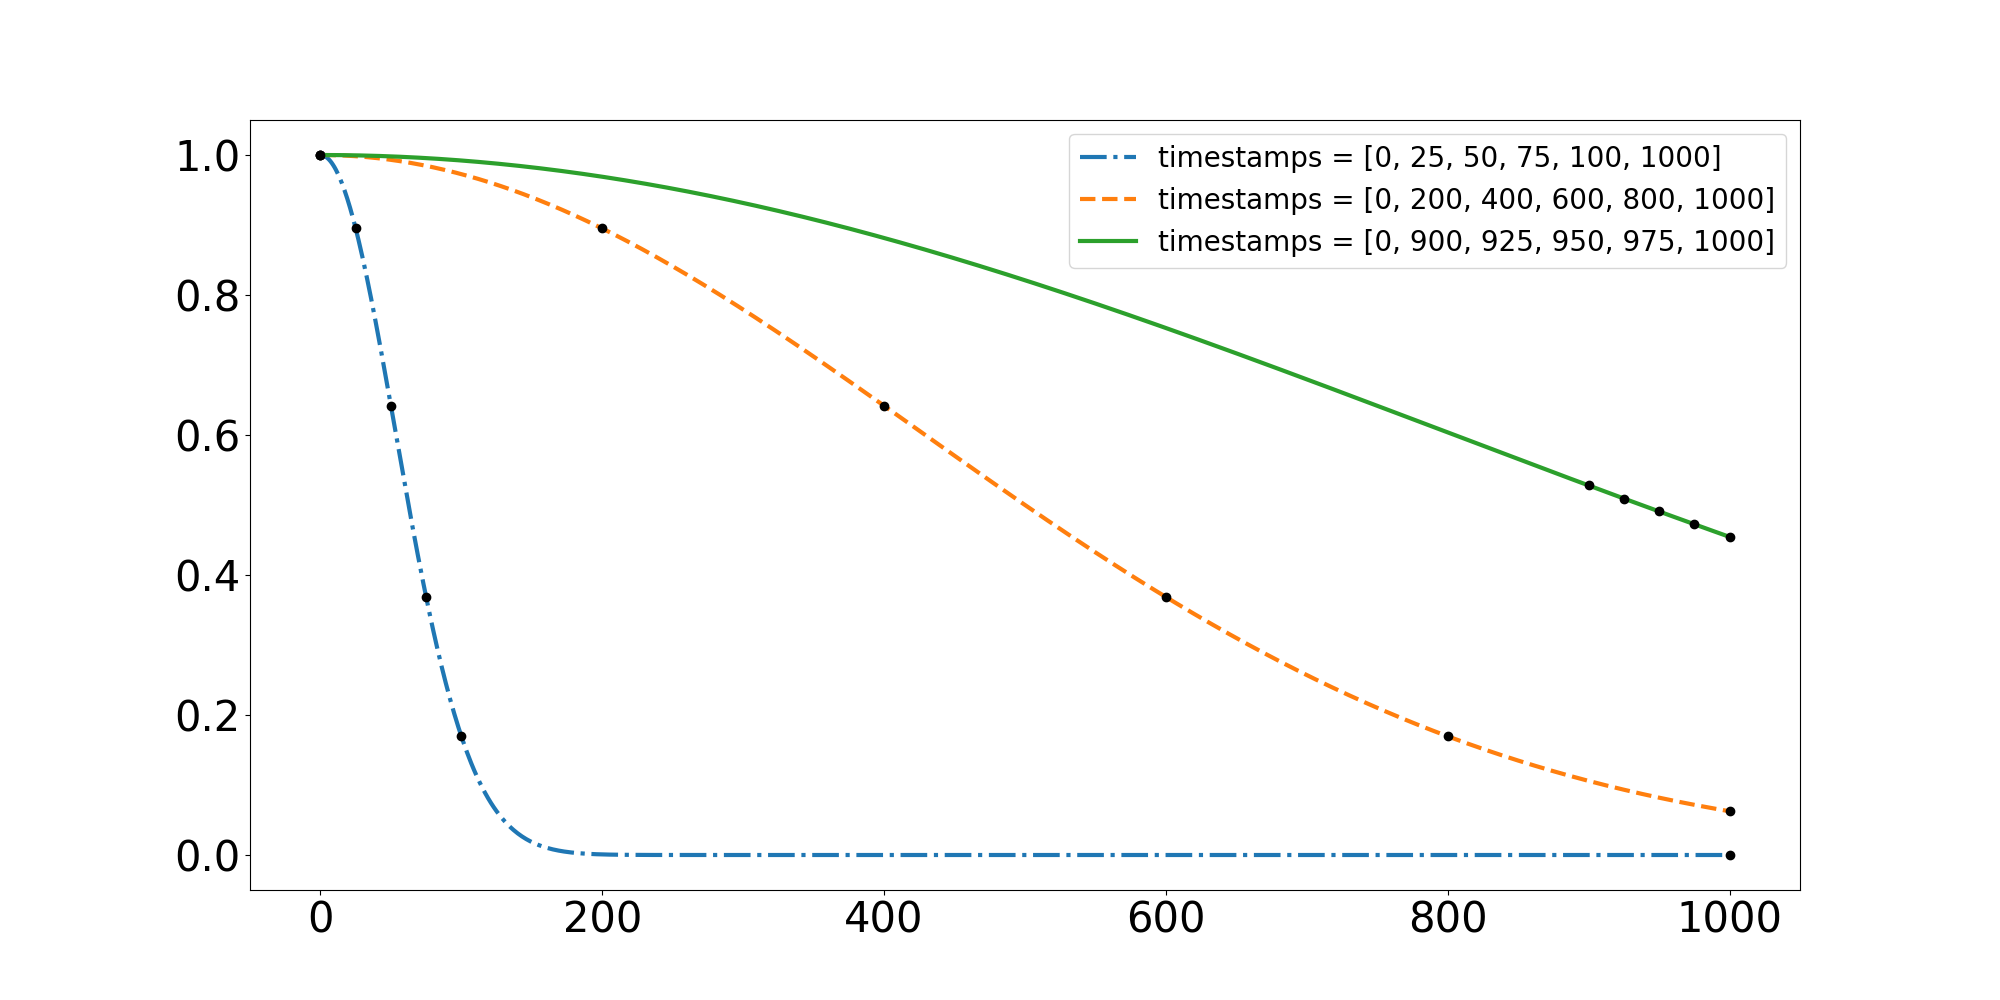
\includegraphics[width=\columnwidth]{weight-function-example.png}
	\caption{Weight functions for three timestamp vectors.}
	\label{fig:weight}
\end{figure}
For each transaction, we evaluate the vector of weights:

\[
w^{tx} = w_{k^{tx}_{opt}}(t^{tx})
\]

Let $X$ be the set of all transactions we consider.
Let $P$ be the set of IP addresses of nodes that appeared in at least one of~$p$ vectors in $X$:

\[
P = \bigcup\limits_{tx \in X} p^{tx}
\]

We define an extended weight vector $v_{tx}$ for each~$tx$ by setting the weight of nodes in $P \backslash p^{tx}$ to zero and sorting the values in the weight vectors w.~r.~t.~the alphabetical order of~$P$.
We then calculate a matrix where an element in $i$-th row and~$j$-th column is the Pearson correlation of the extended weight vectors $v_{tx_i}$ and~$v_{tx_j}$.
This matrix can supposedly be transformed into a block-diagonal matrix with blocks (clusters) corresponding to transaction sources.
To reveal the clusters, we use spectral co-clustering~\cite{Dhillon2001} implemented in the Python \texttt{sklearn.cluster.bicluster} module~\cite{scikit-learn, scikitlearn2018}.
Given an input matrix $A$, the algorithm forms $A_n$ as follows:

\[
A_n = R^{-1/2}AC^{-1/2}
\]

Where $R$ is the diagonal matrix with entry $i$ equal to $\sum_{j} A_{ij}$, and~$C$ is the diagonal matrix with entry $j$ equal to $\sum_{i} A_{ij}$.
This defines the singular value decomposition (SVD) of the normalized matrix $A_n$.
The $l$ = $\lceil \log_2 k \rceil$ singular vectors $u_2,\dots,u_{l+1}$ and $v_2,\dots,v_{l+1}$ of $A_n$ may be used to solve a real approximation of the minimal cut problem.
Let $U$ be a matrix with columns $u_2,\dots,u_{l+1}$, and similarly for $V$ and $v_2,\dots,v_{l+1}$.
Then $Z$ is defined as:

\[
Z = 
\begin{bmatrix}
R^{-1/2} & U \\
C^{-1/2} & V
\end{bmatrix}
\]

The rows of~$Z$ are then clustered using the k-means algorithm to obtain the desired partitioning.


\subsection{Measuring clustering quality}

We use the Rand score as an external metric of clustering quality (see~\cite{Amigo2009}, Section~4.2).
A clustering algorithm decides for each pair of elements, whether to put it in the same cluster.
Let $SS$,~$SD$,~$DS$, and~$DD$ be the numbers of transaction pairs defined as follows:
\begin{itemize}
	\item SS: same cluster, same category\footnote{Here we consider two categories: "our" and "foreign" transactions.} (our transactions in one cluster);
	\item SD: same cluster, different category (our and foreign transactions in one cluster);
	\item DS: different cluster, same category (our transactions in different clusters);
	\item DD: different cluster, different category (our and foreign transactions in different clusters).
\end{itemize}

The Rand score reflects the proportion of right decisions:

\[
R = \frac{SS + DD}{SS + SD + DS + DD}
\]

Note that this assessment only considers clusters with "our" transactions, because we do not know whether any two "foreign" transactions should have been assigned to the same cluster.

We parameterize this metric with the minimal number of our transactions in a cluster required to consider this cluster in the calculation.
In our experiments, we only consider clusters with at least two of our transactions.
With no such threshold, large clusters with one of our transactions disproportionately increase $DD$ and bring the score close to $1.0$, which does not reflect the subjective amount of information an adversary acquires.


\subsection{Measuring the degree of deanonymization}

We measure the success of the attack using a quality score based on the \textit{anonymity degree}~\cite{Diaz2002}.
The goal is to assign to each transaction a probability that it originates from~$S_{control}$.
Initially, all transactions have equal probabilities.
The attacker adjusts the probabilities based on clustering results.
The anonymity degree measures the amount of information the attacker gains.

Let $p_i$ be the probability that a transaction~$i$ originates from~$S_{control}$.
$K$ is the total number of transactions.
The entropy is calculated as:

\[
H = -\sum_{i=1}^K p_i log_2(p_i)
\]

The maximum entropy is:

\[
H_{max} = log_2(K)
\]

The anonymity degree is defined as:

\[
d = \frac{H}{H_{max}}
\]

Our goal is to put transactions that originate from one target source $S_{control}$ to one cluster.
Out of~$K$~captured transactions, $k$ are issued from~$S_{control}$.
For each transaction~$i$, the a priori probability of having originated from~$S_{control}$ is $p_i = k / K$.

We then divide all transactions into clusters.
However, multiple clusters may correspond to~$S_{control}$.
To account for this, each cluster is assigned a \textit{weight} that reflects how likely this cluster represents $S_{control}$.
Consider an example.
The attacker captures $10$~transactions $t_0, \dots, t_9$.
Five of them, $t_0, \dots, t_4$, originate from the target source~$S_{control}$.
The clustering algorithm yields three clusters: $c_a = \{t_0, t_1, t_2, t_3\}, c_b = \{t_4, t_5, t_6, t_7\}, c_c = \{t_8, t_9\}$.
The attacker knows that $t_0$ and~$t_4$ originate from~$S_{control}$ and assigns a weight of~$0.5$ to clusters $c_a$ and~$c_b$, and a weight of~$0$ to cluster~$c_c$.
Therefore, the total "probability weight" of transactions from $S_{control}$ is distributed evenly among $c_a$ and~$c_b$ ($t_0, \dots, t_7$).
Note that the true distribution is $1$ for transactions $t_0, \dots, t_4$ and~$0$ for all others.

Finally, we calculate the \textit{adjusted} anonymity degree accounting for cluster weights.
We calculate the median square error~$e$ between the vectors of probabilities $p_i$ derived by the attacker and the actual probabilities.
The adjusted anonymity degree is defined as follows:

\[
d_{adj} = 1 - (1 - e) \times (1 - d)
\]

Consider two edge case examples.
If $e = 0$ (the attacker correctly guessed the~$S_{control}$ cluster), $d_{adj} = d$.
If $e = 1$ (the attacker's cluster weights do not at all reflect the reality), $d_{adj} = 1$ (the system retains full anonymity).


\section{Implementation details}

We use a modified Bitcoin network probing tool \texttt{bcclient}~\cite{Pustogarov2017} to maintain parallel connections to peers and log incoming messages.
Multiple parallel connections increase our chance to be among the first peers to learn about a new transaction despite broadcast randomization.
The tool is relatively easy to adapt for usage with Dash and Zcash, which mostly inherit the networking layer from Bitcoin Core.
We re-compile \texttt{bcclient} with modified constants (port numbers, protocol magic bytes, DNS seeder addresses).
For Monero, which is not based on the Bitcoin~Core codebase, we modify the reference implementation (\texttt{monerod}).
We add the required logging and disable the built-in limits on the total bandwidth and artificial delays between network requests.

For each transaction announcement, we log the transaction hash, the IP that announced it, and the timestamp of this event.
We only log \texttt{inv} messages, and never continue with the \texttt{getdata} -- \texttt{tx} exchange.
For selected experiments on the Bitcoin testnet, we also log \texttt{addr} messages.
Address announcements allow us to infer the set of most probable IP addresses that correspond to each transaction cluster.
We use Python scripts to process the log, save the data in a more compact JSON format, analyze it, and visualize the results.


\section{Experimental evaluation}

The outline of our experiment is as follows:

\begin{enumerate}
	\item collect a fresh list of live peers;
	\item establish multiple parallel connections to them;
	\item launch the listening nodes and start logging \texttt{inv} and \texttt{addr} messages;
	\item launch two nodes $S_{learn}$ and~$S_{control}$;%, so that their initial \texttt{addr} advertisements are logged;
	\item issue two series of transactions: the learning set from~$S_{learn}$ and the control set from~$S_{control}$;
	\item for each considered number $N$ of first propagations, calculate the transaction correlation matrix;
	\item run the clustering algorithm with various assumed average numbers of transactions per cluster;
	\item choose the best clustering by Rand score based on the "learning" set;
	\item in the best clustering, assign the cluster weights proportionally to the distribution of known transactions from~$S_{control}$;
	\item assign zero probability of being in~$S_{control}$ to transactions from~$S_{learn}$;
	\item re-distribute the probability weight among transactions in each cluster;
	\item calculate the final adjusted anonymity score;
	\item re-arrange the clusters such that high correlation values are close to the main diagonal;
	\item visualize the results.
\end{enumerate}

We visualize the results with heatmaps.
We assign a color to each element of the correlation matrix.
A darker color at the intersection of the~$i$-th row and~$j$-th column represents a stronger correlation of weight vectors of~$i$-th and~$j$-th transactions.
The heatmap is diagonally symmetric by definition: each vector is perfectly correlated with itself.
We permute rows and columns such that the highly correlated elements are close to the main diagonal.
We expect such permutation to reveal the block-diagonal structure of the matrix.


\subsection{Results for desktop wallets}

We evaluate our method by clustering our own transactions in Bitcoin (testnet and mainnet) and Zcash.
For these experiments, we log the traffic for $15$~minutes.
For Dash and Monero, we run the clustering algorithm without calculating the anonymity degree.
We obtain clearly visible clusters, which indicated that our approach is applicable to these cryptocurrencies as well.
The experiments on the Bitcoin mainnet deliberately do not attempt to occupy all connection slots and operate only on a subset of~$1\,000$~nodes (out of approximately $10\,000$~nodes reachable at any given time~\cite{Bitnodes}).
In this section, we refer to the node that logs the incoming messages as the \textit{listener}.
Following the terminology of~\cite{Biryukov2014}, \textit{servers} are peers that accept incoming connections.

% California: experiment-1541509693
% Tokyo: experiment-1541511845
% Frankfurt: experiment-1541513977
% 3-experiment: experiment-1541516997
\begin{table*}[!t]
	\normalsize
	\caption{Experimental results of transaction clustering for Bitcoin testnet and Zcash.}
	\centering
	\begin{tabular}{|l|l|c|c|c|c|c|}
		\hline
		Network & Listener & Anon\@. deg. & Servers & Avg free slots & Tx \texttt{inv}s & \texttt{addr}s \\
		\hline
		Bitcoin test & California & $0.83$ & $1\,141$ & $64$ & $139$ & $402$ \\
		Bitcoin test & Tokyo & $0.80$ & $1\,128$ & $64$ & $193$ & $414$ \\
		Bitcoin test & Frankfurt & $0.72$ & $1\,137$ & $64$ & $172$ & $403$ \\
		Bitcoin test & combined & $0.63$ & $1\,154$ & $63$ & $250$ & $1\,321$ \\
		Bitcoin main & Frankfurt & $0.88$ & $1\,000$* & $25$* & $3\,238$ & $11\,300$ \\
		Zcash & Frankfurt & $0.86$ & $206$ & $36$ & $62$ & $1\,086$ \\
		\hline
	\end{tabular}
	\label{tab:results}
\end{table*}

\subsubsection{Bitcoin testnet}

We perform four experiments on the Bitcoin testnet using listeners in different geographical locations: Frankfurt (Germany), Tokyo (Japan), and North California (the US).
We conduct three experiments with each of the listeners and the fourth experiment using all listeners simultaneously.
To use multiple listeners in one experiment, we distribute live peers equally among the three listeners.
Each listener connects only to the peers from its chunk of the list.
We then merge the log files.
The fourth experiment measures the advantage an adversary gains from using geographically distributed listeners.
Each listener attempts to establish $117$~connections to each assigned peer.

In each experiment, we issue two sets of test transactions (the learning and the control sets) containing $30$~transactions each from computers located in Luxembourg.
We denote $10$~transactions from the control set as "known" to estimate the anonymity degree.

The number of live peers collected by each of the listeners is close, which indicates that we obtain a complete view of the network.
The number of received transactions varies little between experiments, whereas the number of \texttt{addr} messages is significantly higher in the multi-listener experiment: \texttt{addr} messages propagate through the network more slowly than transactions.
The average number of available connection slots is independent of the location of the listener.

The anonymity degree calculated on our own transactions indicates a substantial loss of privacy (Table~\ref{tab:results}).
The "*"~sign in the table indicates the experiments where we only connected to a subset of available nodes.
The joint experiment with three geographically distributed listeners gained the best results with an anonymity degree of~$0.63$.
Out of the three single-listener experiments, only the Frankfurt experiment shows a lower anonymity degree.
We explain it by a small geographical distance between the listener and the transaction source.
The results are presented in Figures~\ref{fig:bitcoin-testnet-california},~\ref{fig:bitcoin-testnet-tokyo},~\ref{fig:bitcoin-testnet-frankfurt}, and~\ref{fig:bitcoin-testnet-combined} (ticks along the axes denote our transaction from the control set).


\begin{figure*}
	\centering
	\begin{minipage}{0.5\textwidth}
		\centering
		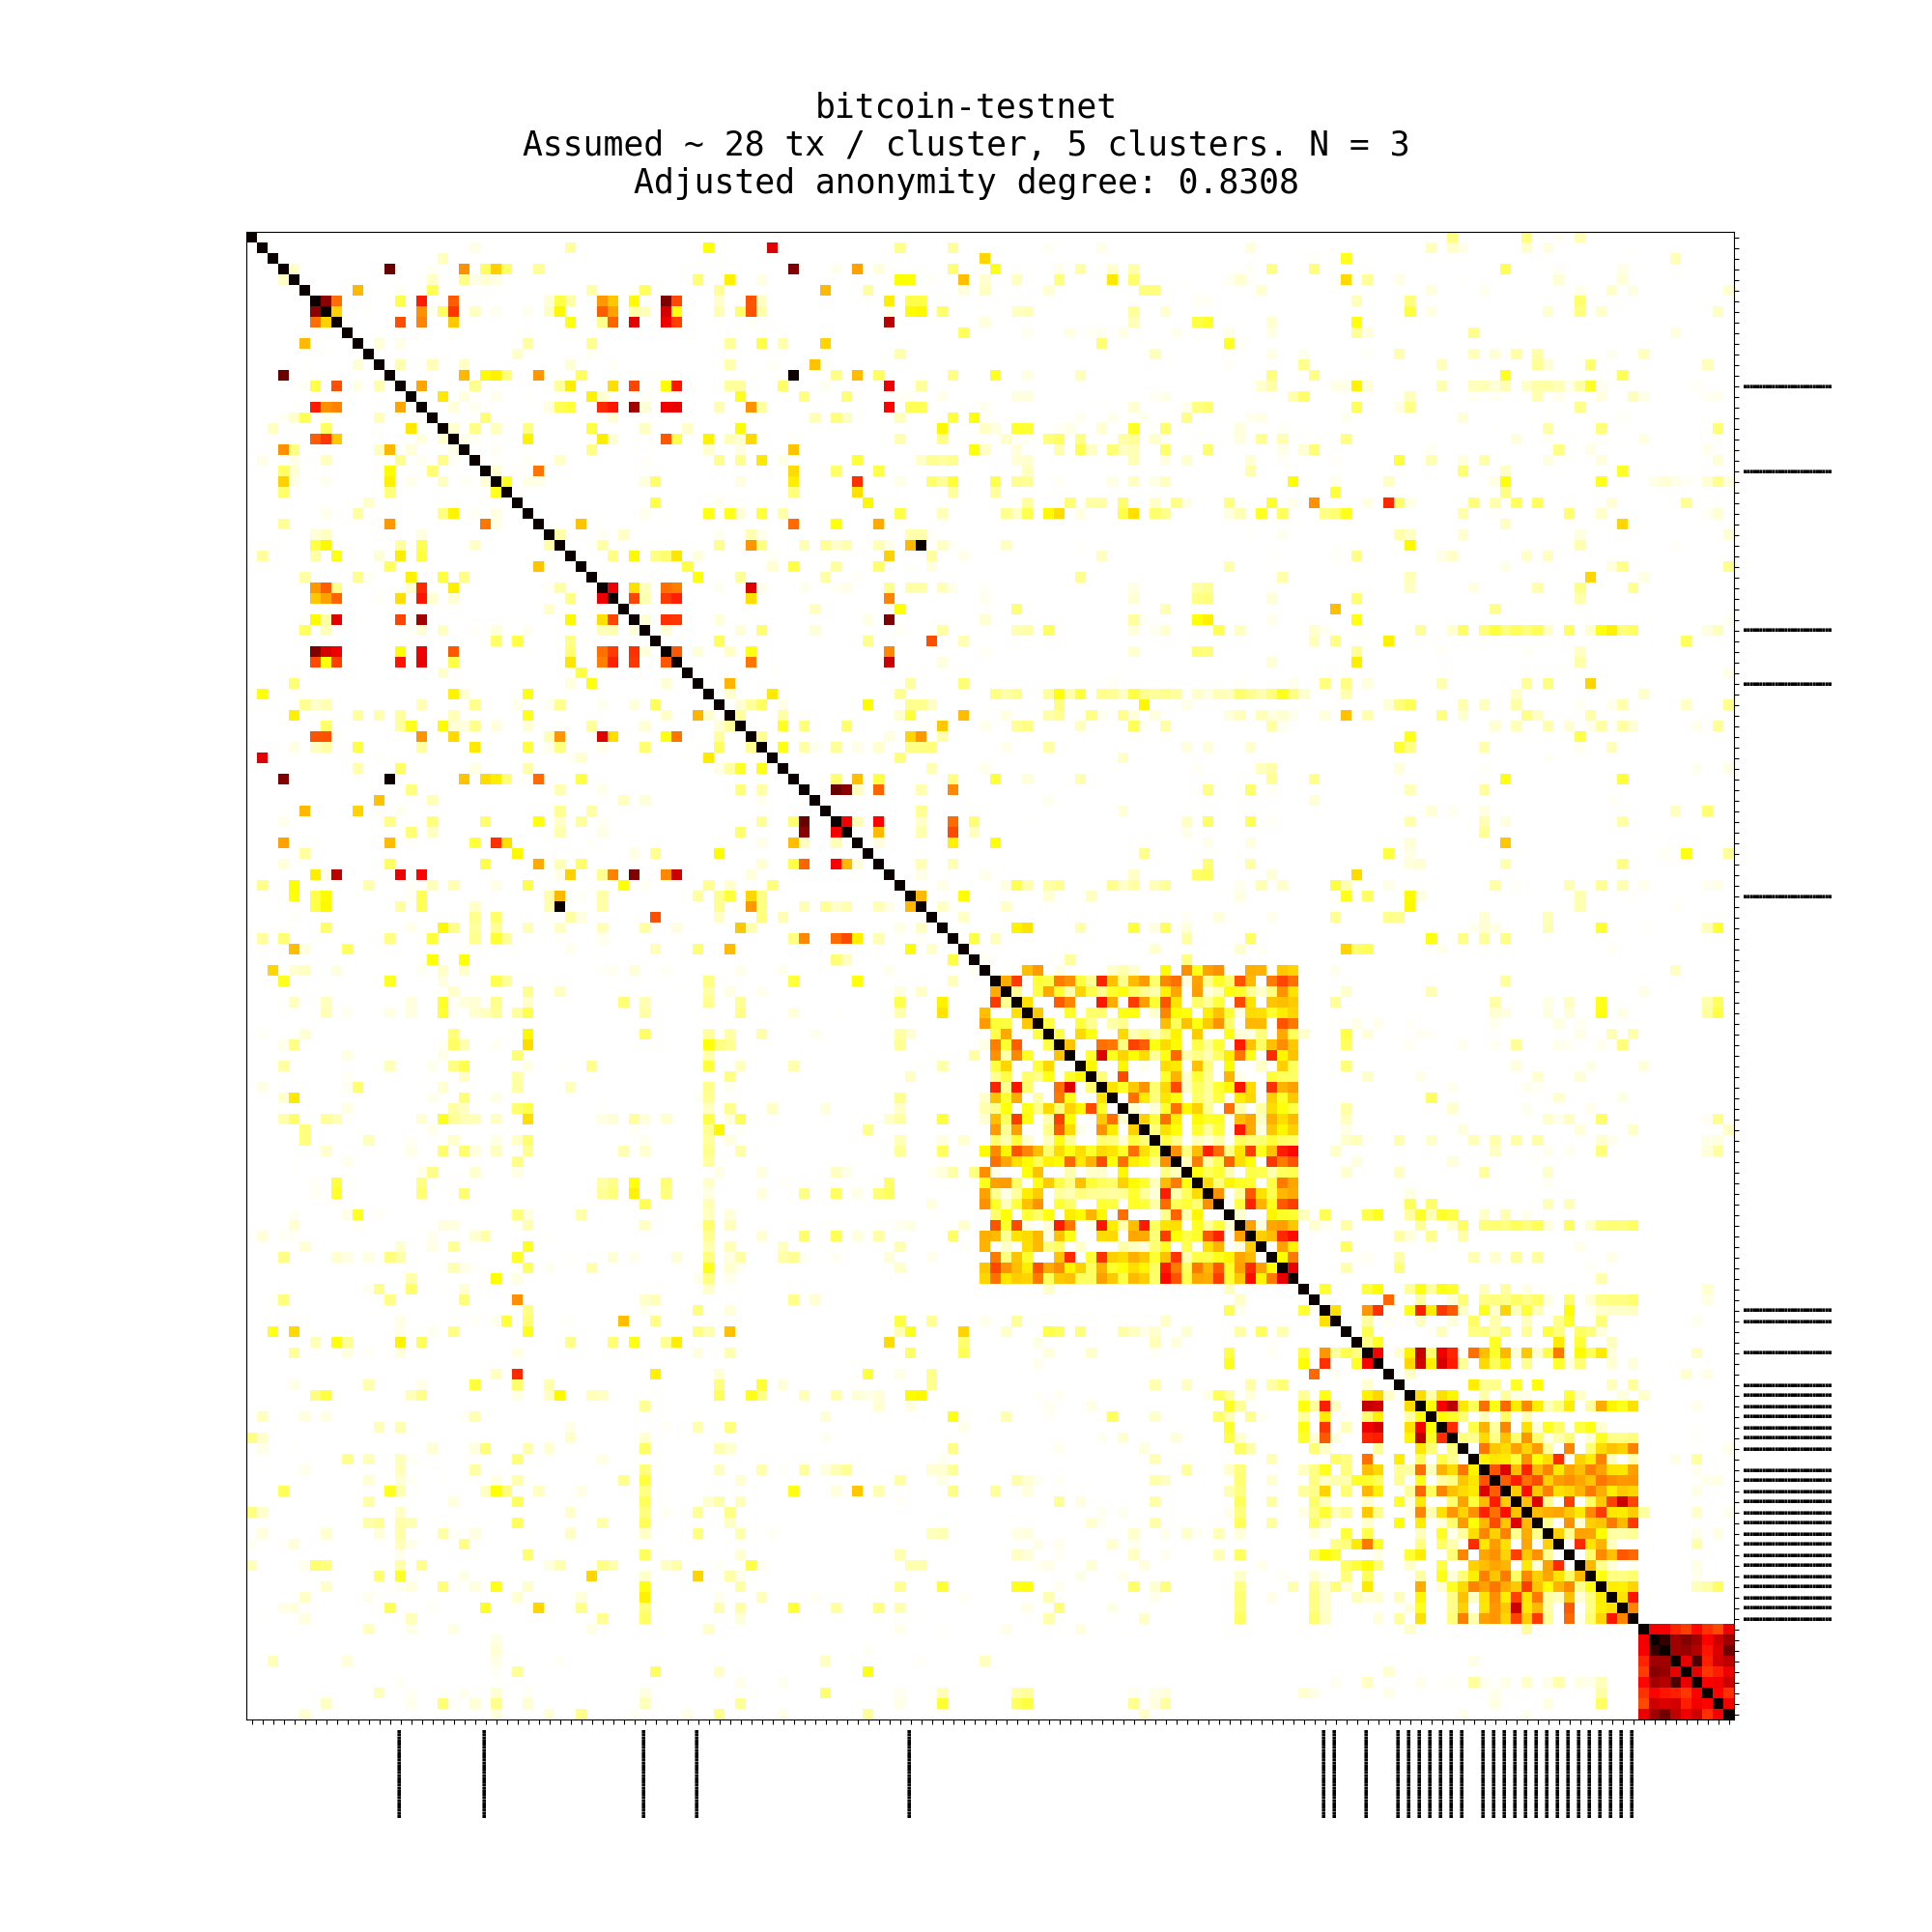
\includegraphics[width=\columnwidth]{bitcoin-testnet-1541509693-California.png}
		\caption{Transaction clustering for Bitcoin testnet (listener in California).}
		\label{fig:bitcoin-testnet-california}
	\end{minipage}\hfill
	\begin{minipage}{0.5\textwidth}
		\centering
		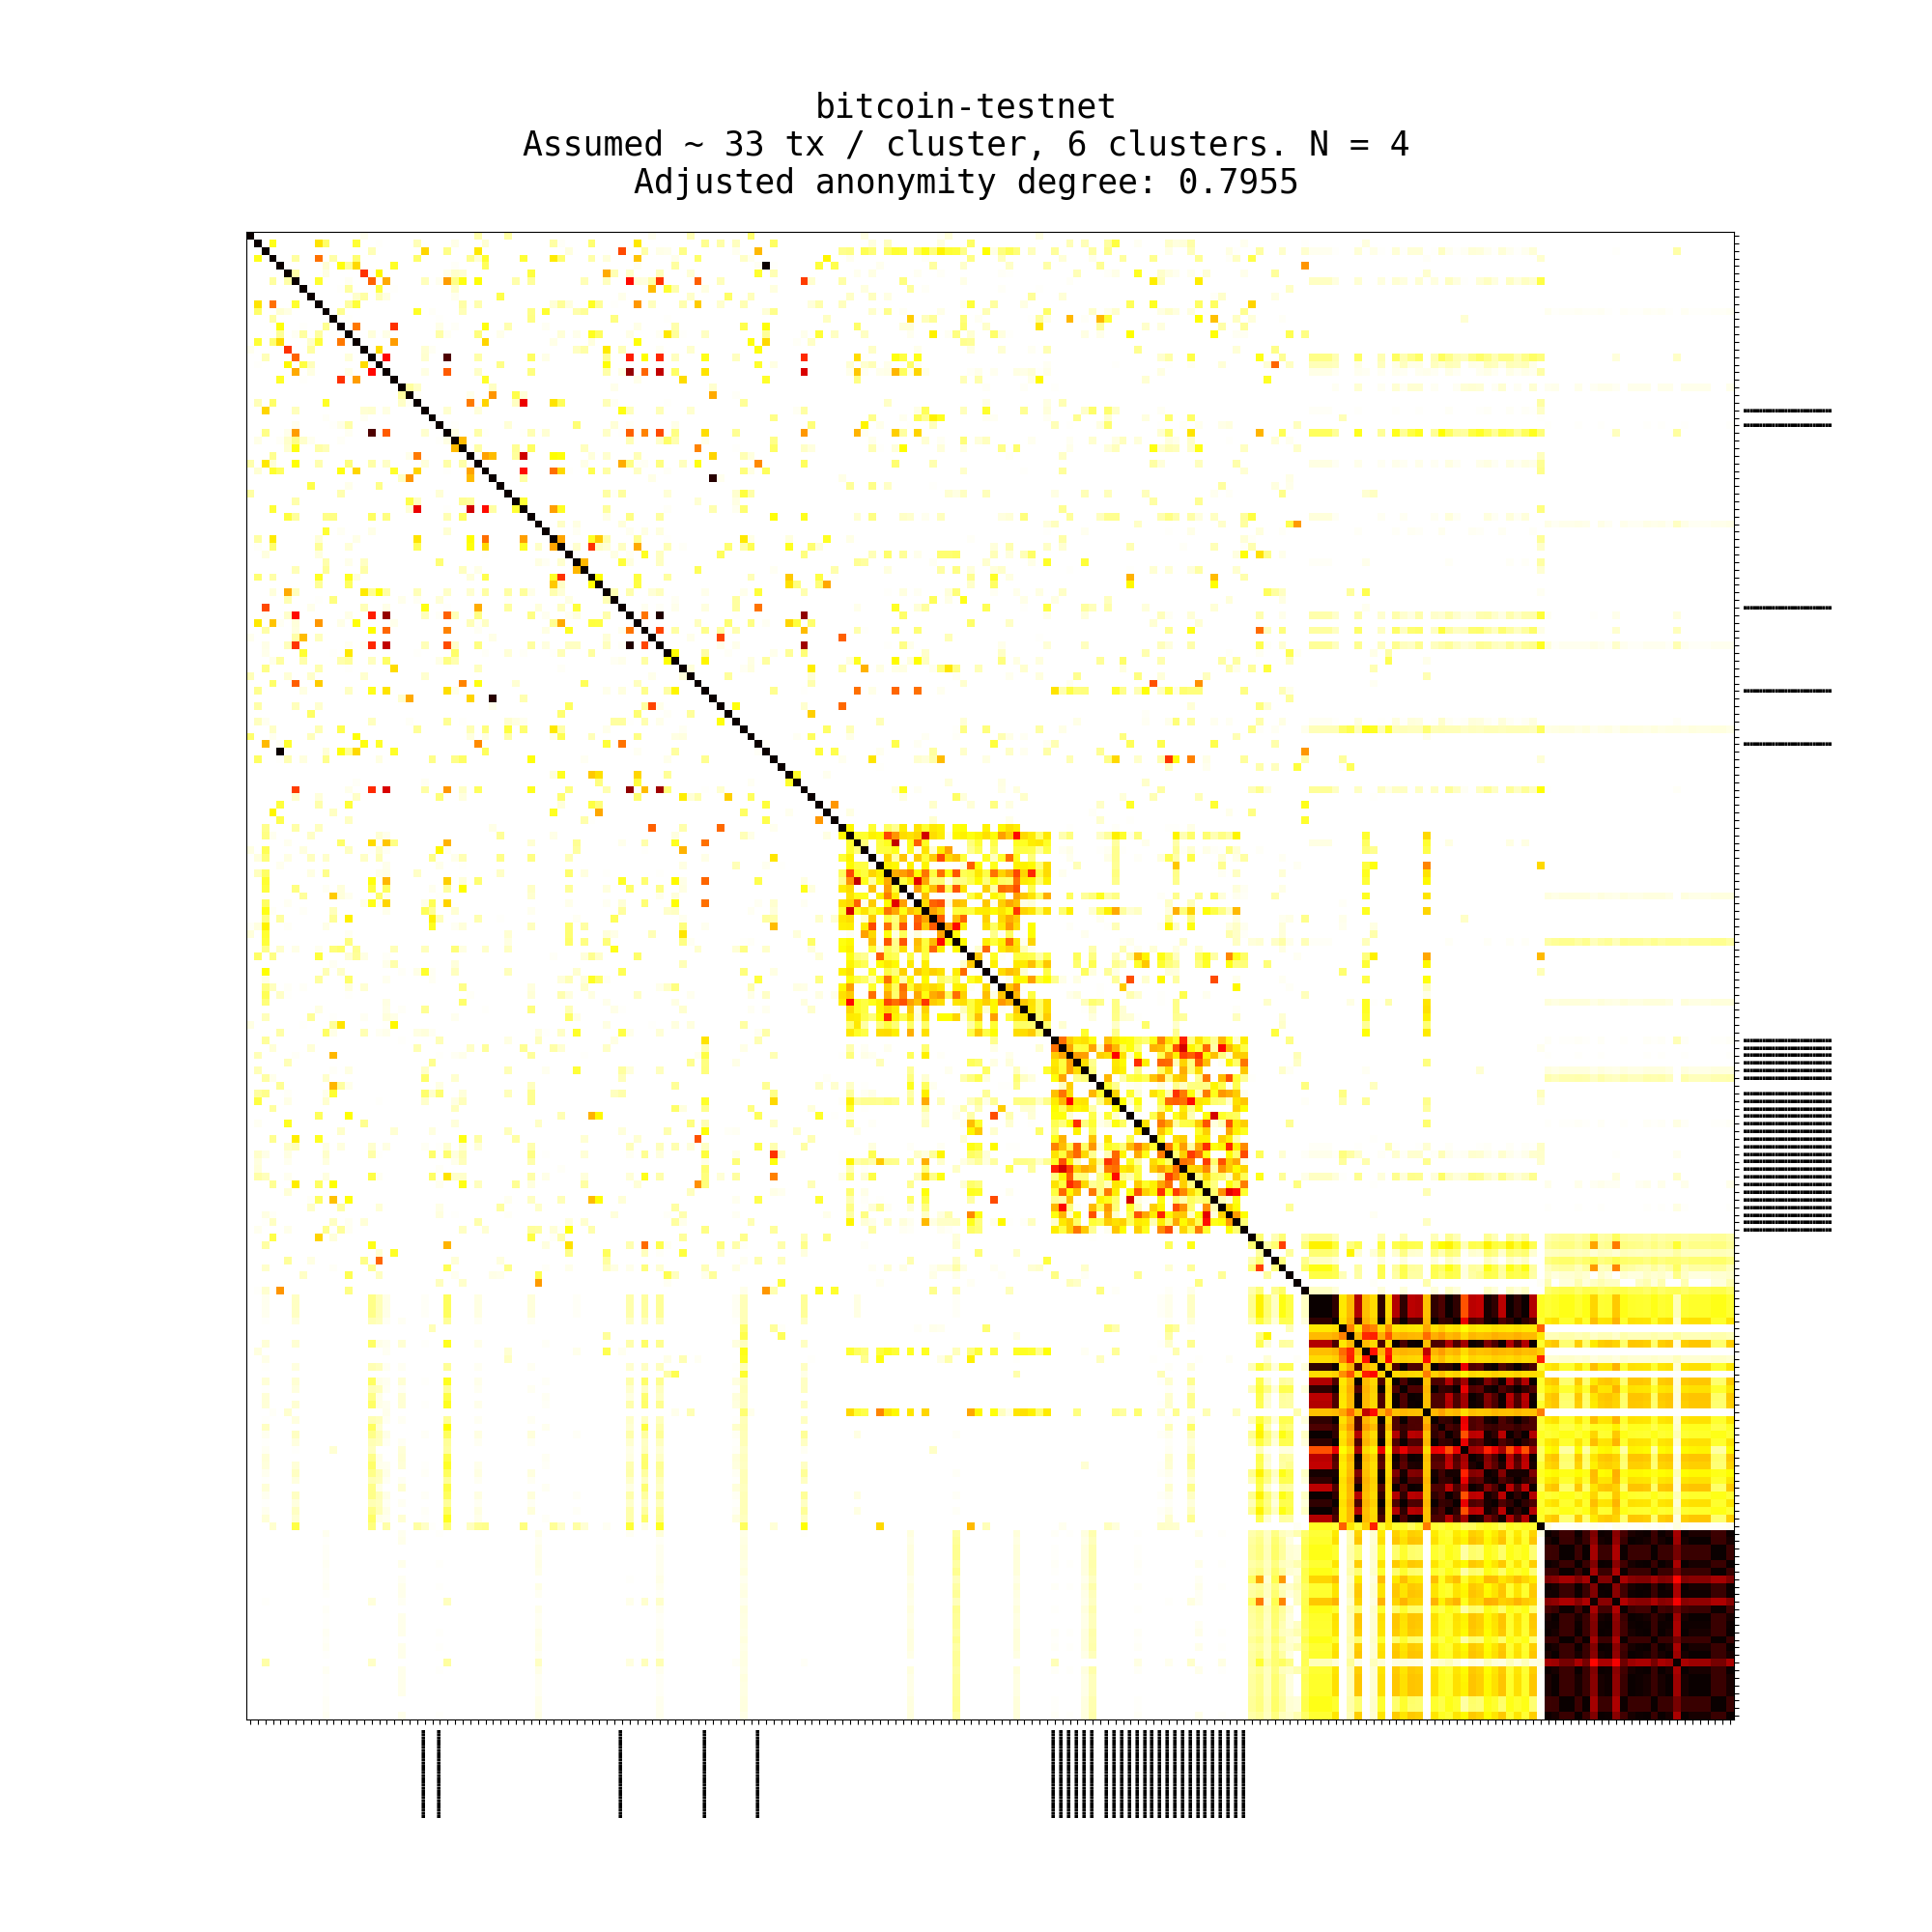
\includegraphics[width=\columnwidth]{bitcoin-testnet-1541511845-Tokyo.png}
		\caption{Transaction clustering for Bitcoin testnet (listener in Tokyo).}
		\label{fig:bitcoin-testnet-tokyo}
	\end{minipage}\hfill
\end{figure*}

\begin{figure*}
	\centering
	\begin{minipage}{0.5\textwidth}
		\centering
		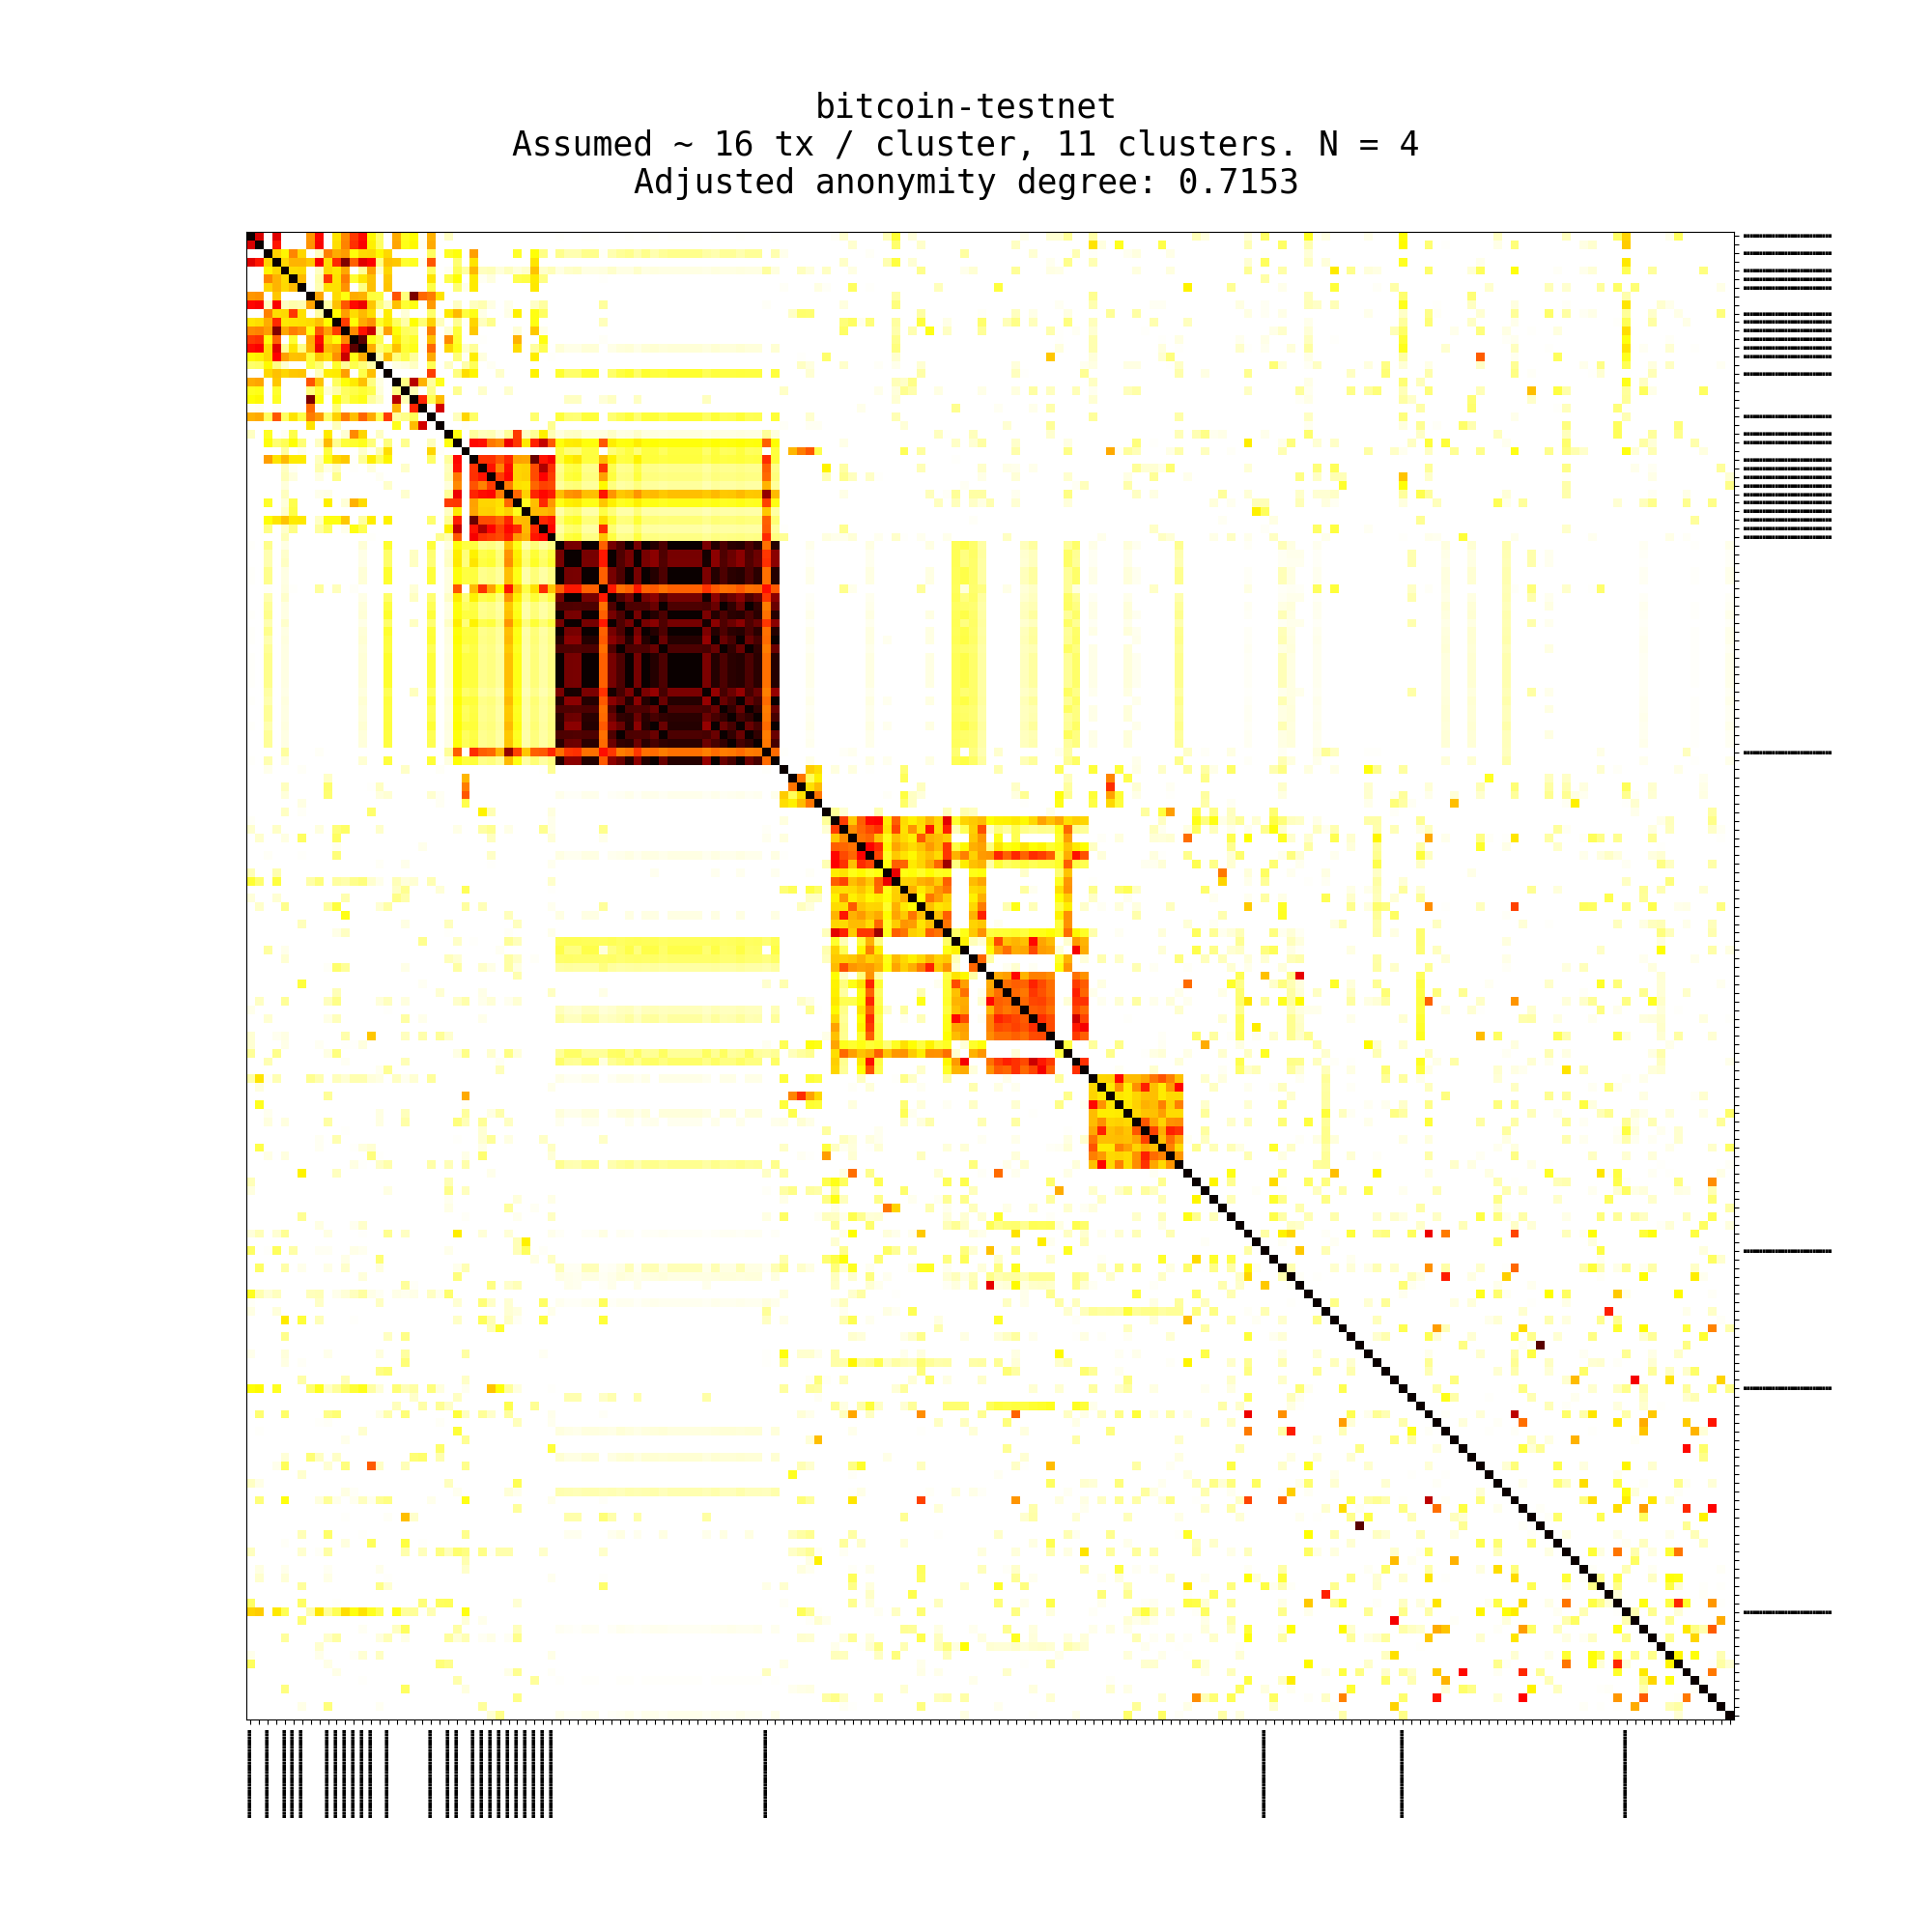
\includegraphics[width=\columnwidth]{bitcoin-testnet-1541513977-Frankfurt.png}
		\caption{Transaction clustering for Bitcoin testnet (listener in Frankfurt).}
		\label{fig:bitcoin-testnet-frankfurt}
	\end{minipage}\hfill
	\begin{minipage}{0.5\textwidth}
		\centering
		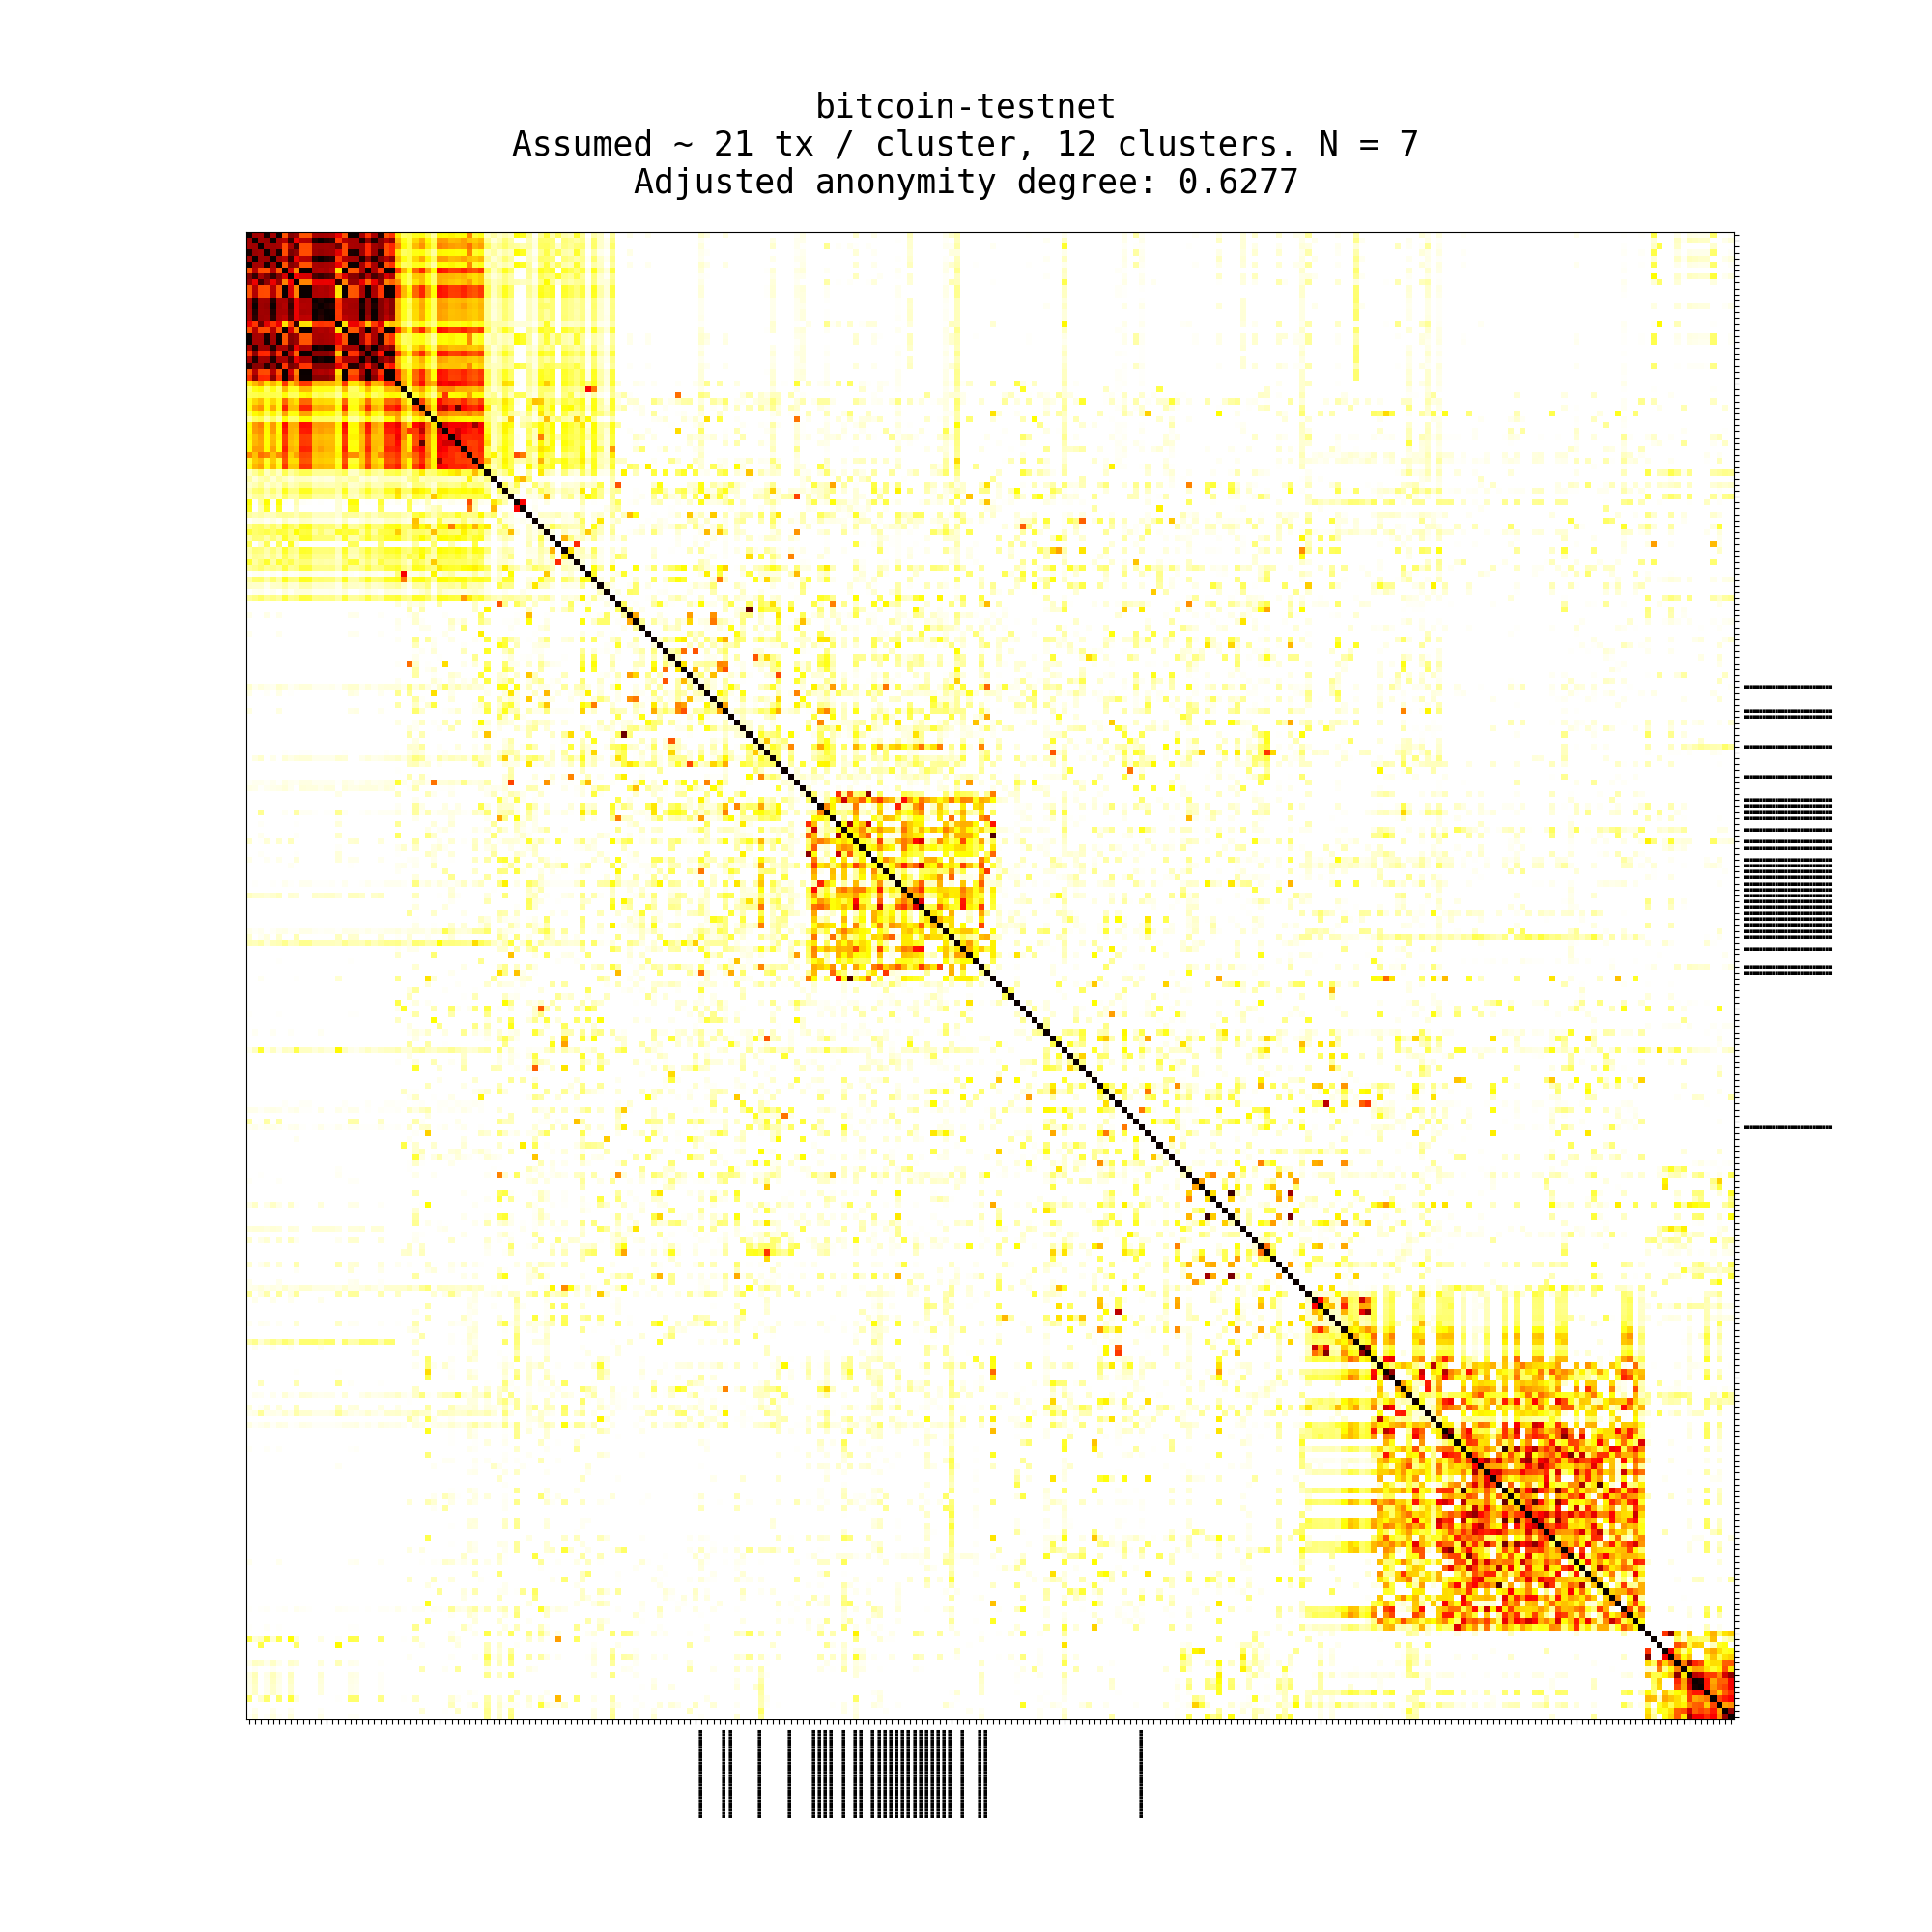
\includegraphics[width=\columnwidth]{bitcoin-testnet-1541516997-combined.png}
		\caption{Transaction clustering for Bitcoin testnet (combined listeners).}
		\label{fig:bitcoin-testnet-combined}
	\end{minipage}\hfill
\end{figure*}


\paragraph{Estimating the original IP}

We use the \texttt{addr} messages to determine (with some level of precision) the IP address of the transaction source.
In our experiments, we first launch the listener and only then launch the issuing nodes.
This allows the listener to capture the \texttt{addr} messages issued by the issuing nodes during bootstrapping.
Address messages propagate through the network more slowly than transactions and are periodically re-broadcast.
A listener can distinguish between \texttt{addr} messages of recently joined nodes and re-broadcasts of older \texttt{addr} messages.
If only one or two nodes announce an IP address, we assume it is a re-broadcast.
If more nodes announce an IP address, we assume that the node has just joined the network or is re-advertising its IP.

We leverage the \texttt{addr} messages as follows.
For each cluster, we determine the IPs of the most "important" nodes, i.e.,~nodes we assume might be the source or its entry nodes.
For each transaction in the cluster, we sum up the weights of all IPs that relayed it to us.
We assume the top $10\%$~of most weighted IPs to be the entry nodes.
The intuition is that the entry nodes are among the first to relay \texttt{addr} messages from the source.
Therefore, we assume that an \texttt{addr} message relayed by a set of IPs that substantially intersects with the entry nodes contains the IP address of the source of the cluster.

We apply this heuristic to the Bitcoin testnet experiments.
We consider the clusters that mostly consist of control transactions.
In three out of four experiments, the actual IP address is among the top five most "important" IPs.
This result indicates that an adversary can narrow down the search for the source IP address to only a handful of IPs.

\subsubsection{Bitcoin mainnet}

We perform one experiment on the Bitcoin mainnet with a listener located in Frankfurt.
The learning and control sets consist of~$20$~transactions each.
Five transactions from the control set are assumed "known" for anonymity degree calculation.

The results are presented in Table~\ref{tab:results} and Figures~\ref{fig:bitcoin-mainnet} and~\ref{fig:zcash}.
The correlation matrix also exhibits the "clustering" behavior, though the anonymity loss is smaller than in for Bitcoin testnet and Zcash.
We explain these weaker results by multiple factors.
First, the Bitcoin mainnet is substantially larger than other networks that we consider.
More transactions in Bitcoin constitute a larger anonymity set.
Second, Bitcoin nodes provide fewer connection slots and often limit the number of slots one IP can occupy.
A low number of parallel connections decreases the probability that our listener learns about a new transaction quickly.
Third, we only establish up to $50$~connections to $1\,000$~peers to avoid disrupting the network, and due to resource constraints.

\begin{figure*}
	\centering
	\begin{minipage}{0.5\textwidth}
		\centering
		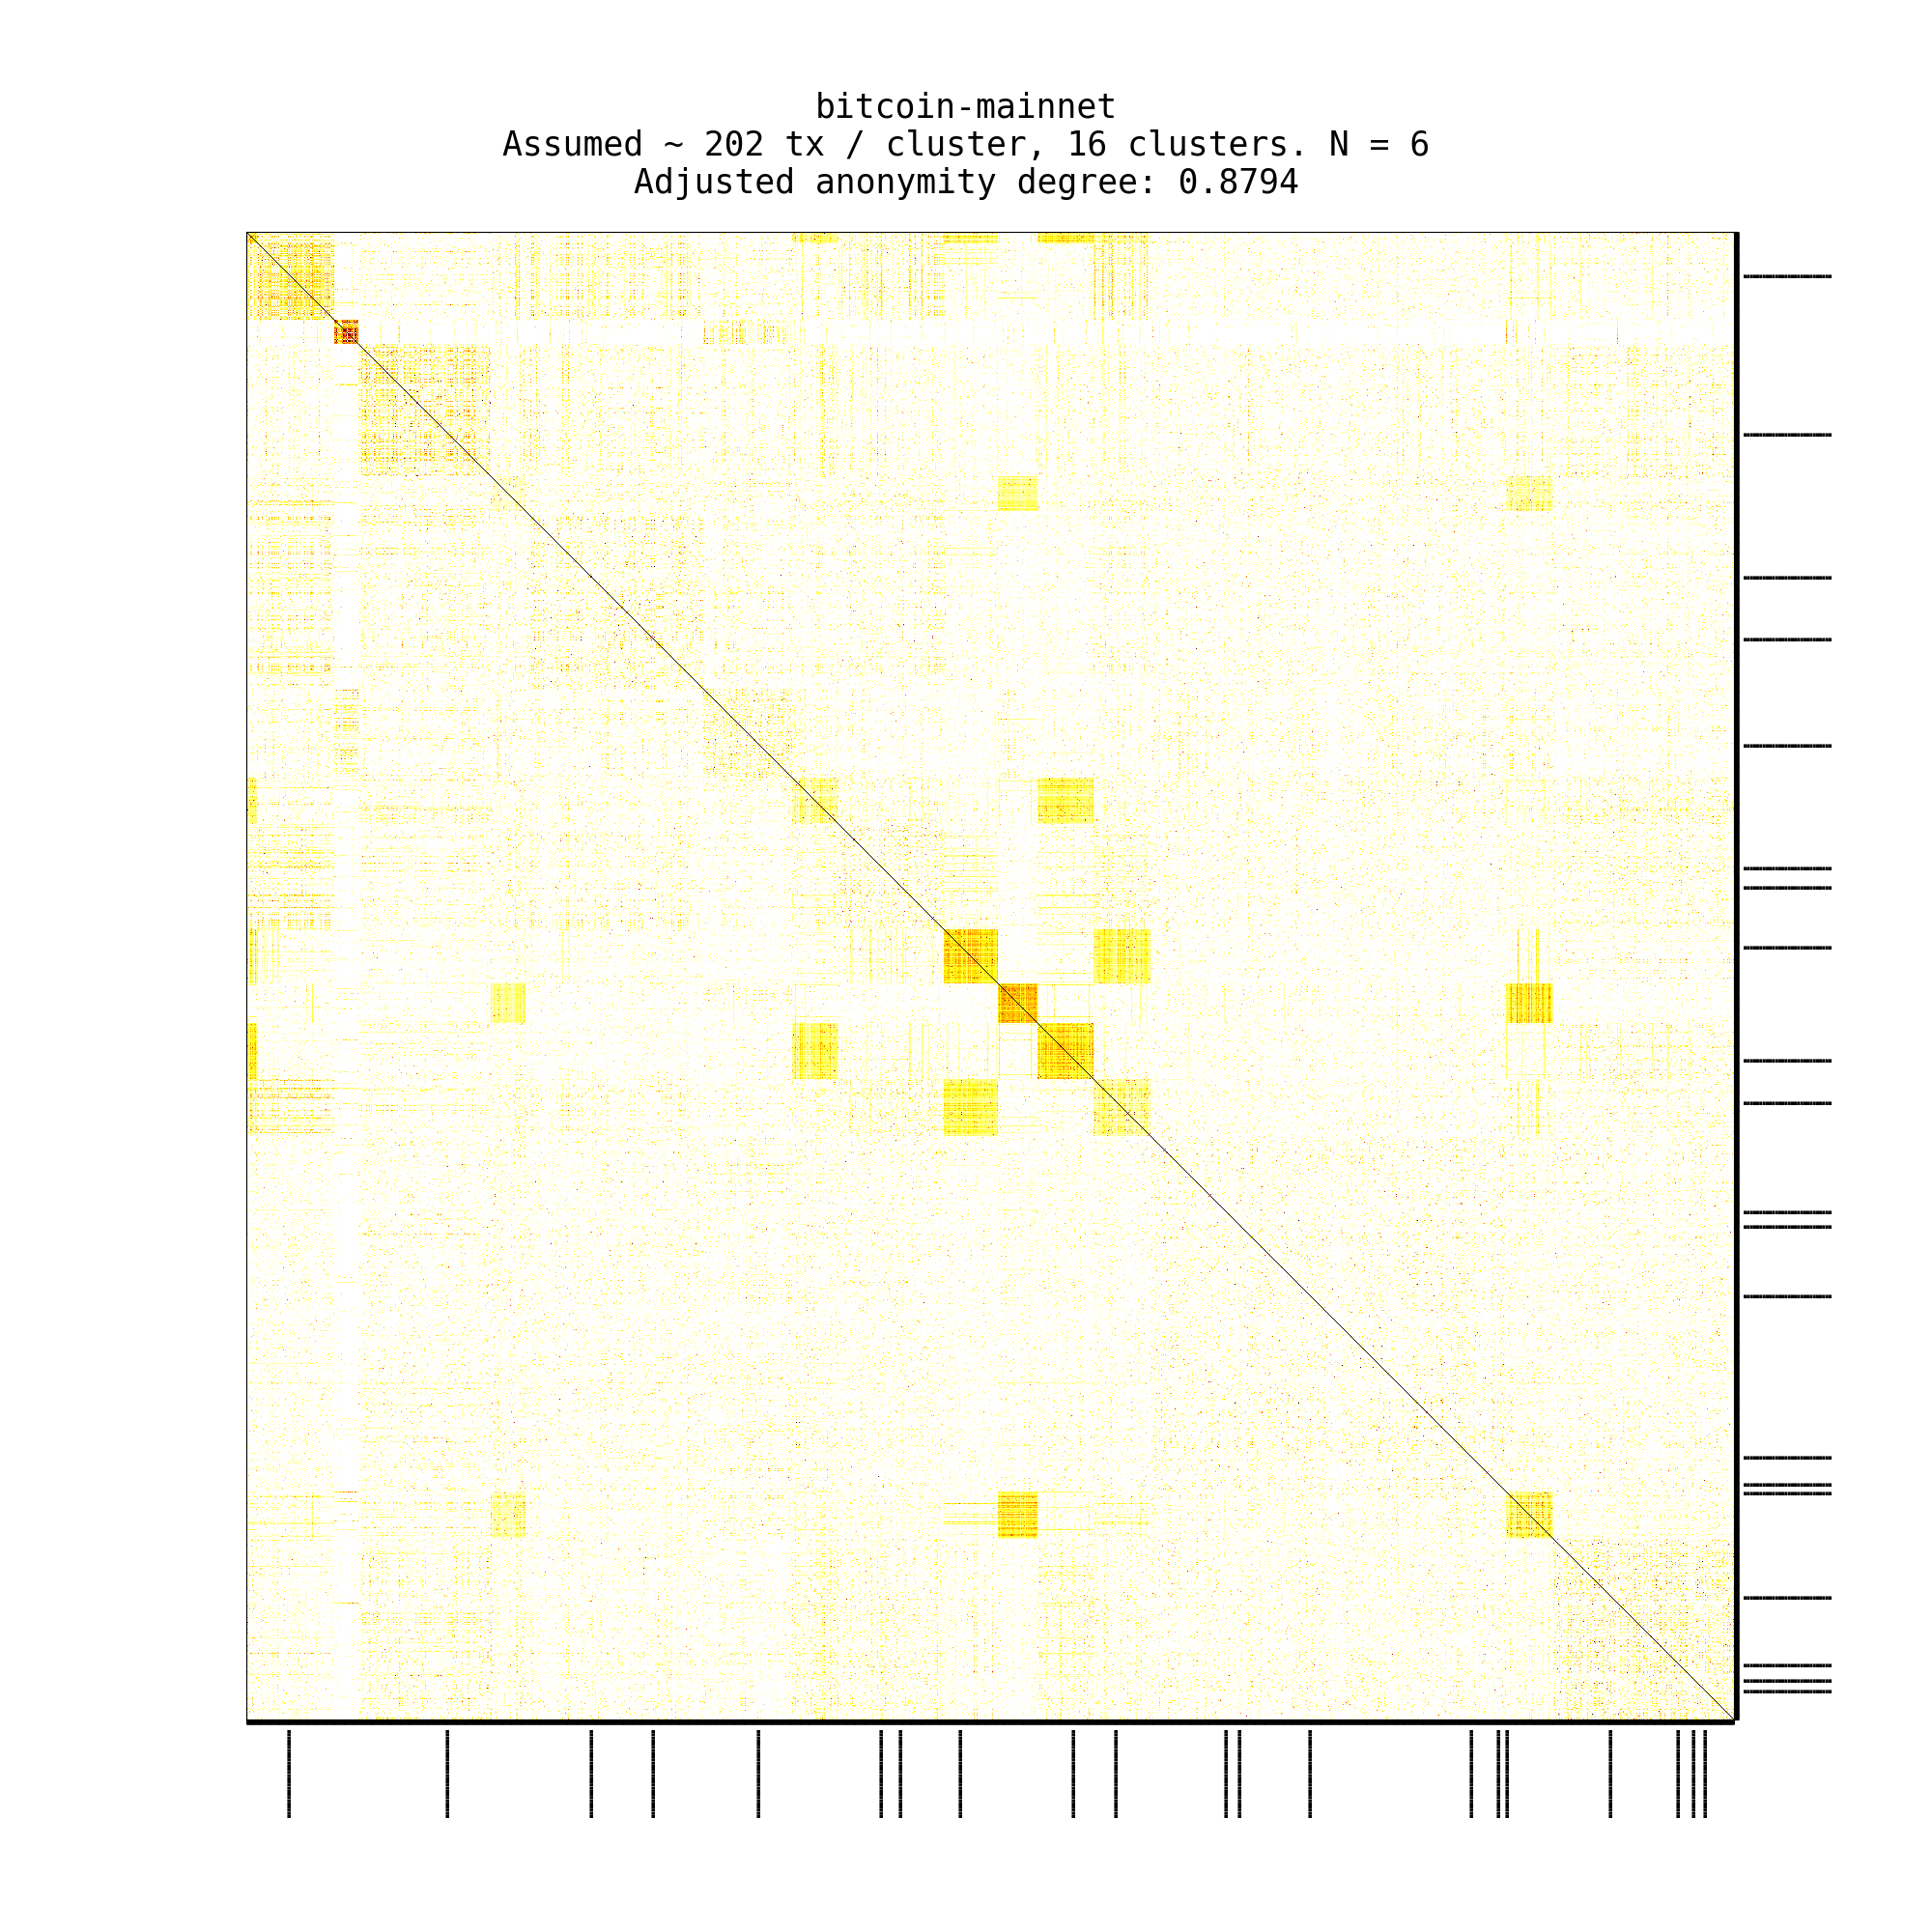
\includegraphics[width=\columnwidth]{bitcoin-mainnet-1542054034-fig-correlations-202-txcl-006-N-Rand-best.png}
		\caption{Transaction clustering for Bitcoin mainnet.}
		\label{fig:bitcoin-mainnet}
	\end{minipage}\hfill
	\begin{minipage}{0.5\textwidth}
		\centering
		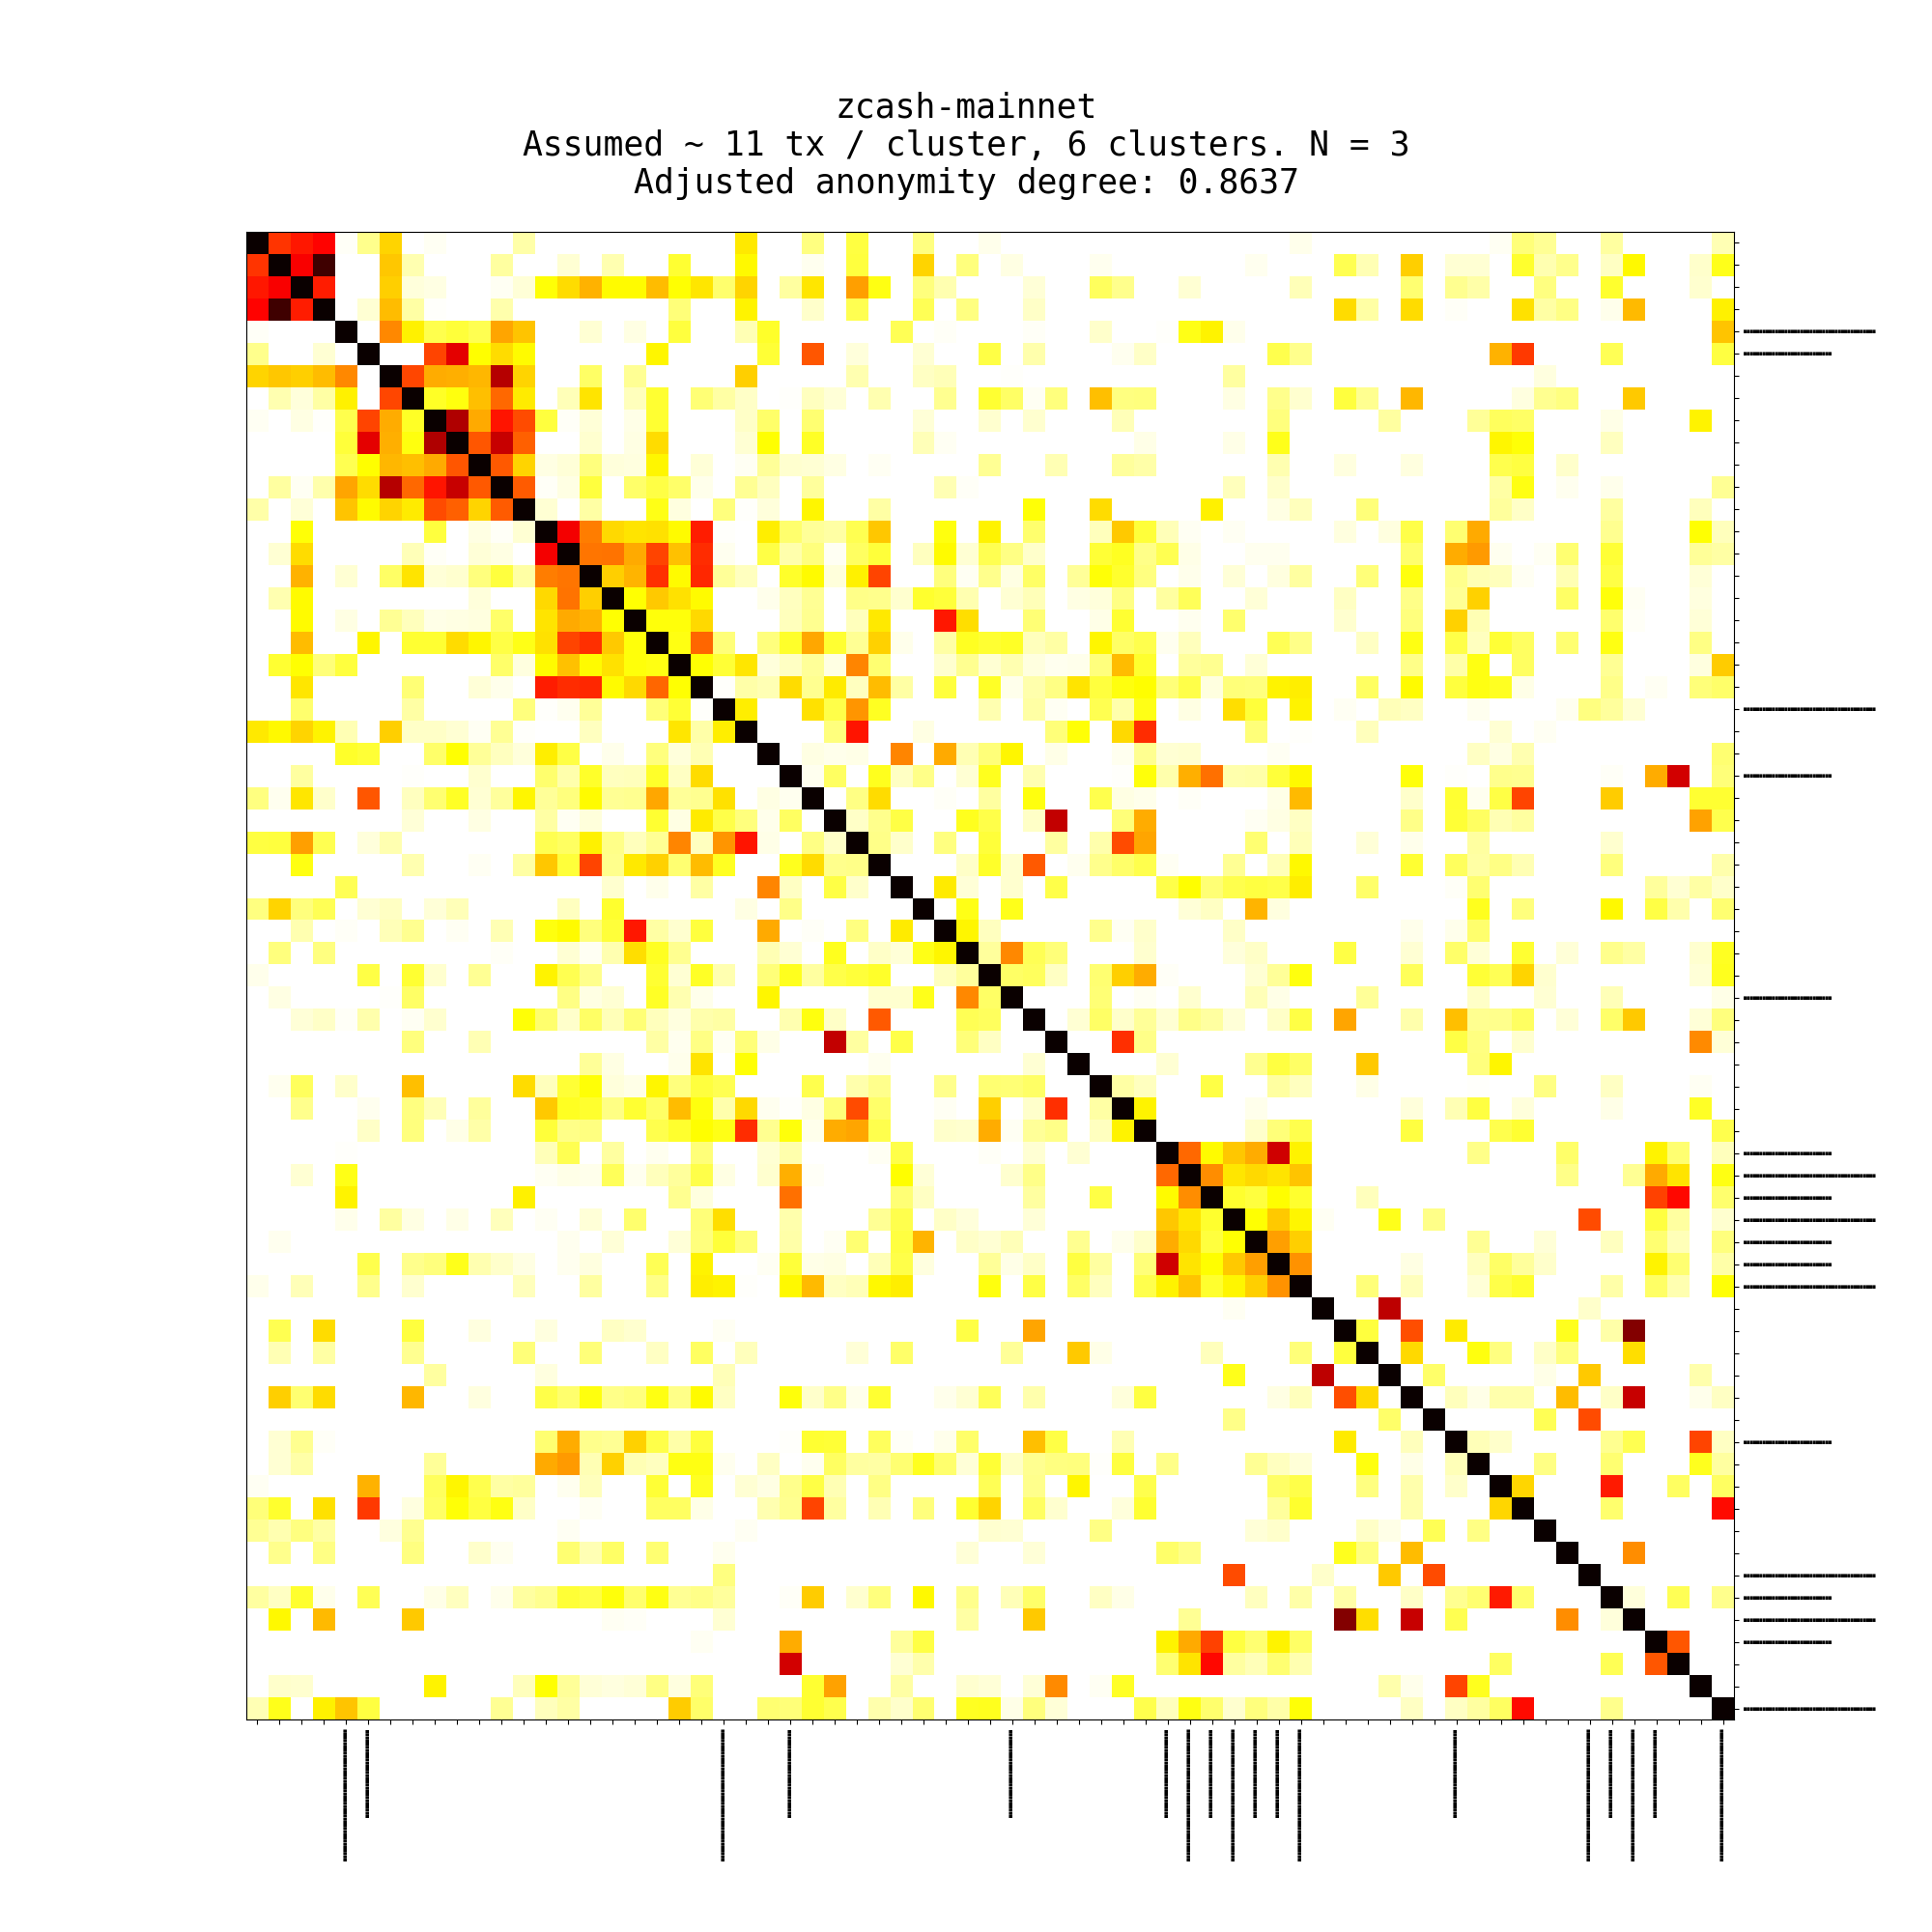
\includegraphics[width=\columnwidth]{zcash-mainnet-1541938472-Frankfurt.png}
		\caption{Transaction clustering for Zcash.}
		\label{fig:zcash}
	\end{minipage}\hfill
\end{figure*}

\subsubsection{Zcash}

Zcash is based on the Bitcoin~Core codebase.\footnote{Bitcoin~Core~version~0.11.2 (commit~7e27892), November~2015.}
As of the time of our experiments (mid-2018), Zcash uses trickling for broadcast randomization, while Bitcoin uses diffusion.
Zcash does not provide privacy by default: zero-knowledge proofs are used only in transactions involving \textit{shielded} addresses~\cite{Kappos2018}.
Most transactions happen between \textit{transparent} addresses and have no added privacy-preserving mechanisms compared to Bitcoin.

We perform one experiment on the Zcash mainnet with a listener located in Frankfurt.
The learning and control sets consist of~$20$ and~$18$~transactions, respectively.
Eight~out of~$18$~control transactions use shielded addresses (transactions from a t-address to a z-address, also known as t-to-z).
We use $6$~control transactions as "known" for anonymity degree estimation.

The results are presented in Figures~\ref{fig:bitcoin-mainnet} and~\ref{fig:zcash}.
T-to-z transactions from the control set are marked with longer ticks.
Note that our method clusters transactions involving both transparent and shielded addresses.

%The Zcash network is much smaller than the Bitcoin testnet.
We notice that Zcash peers offer far fewer connection slots on average: $36$~compared to $64$~on Bitcoin testnet (Figures~\ref{fig:free-slots-bitcoin} and~\ref{fig:free-slots-zcash}).
Many servers only allow fewer than ten connections.
These results may reflect a larger share of \textit{protected} nodes in Zcash.
Protected nodes use firewalls or other network-level mechanisms to limit the number of connections from each IP\@.
However, an adversary can overcome this limitation by purchasing IP addresses from a cloud provider.

\begin{figure*}
	\centering
	\begin{minipage}{0.5\textwidth}
		\centering
		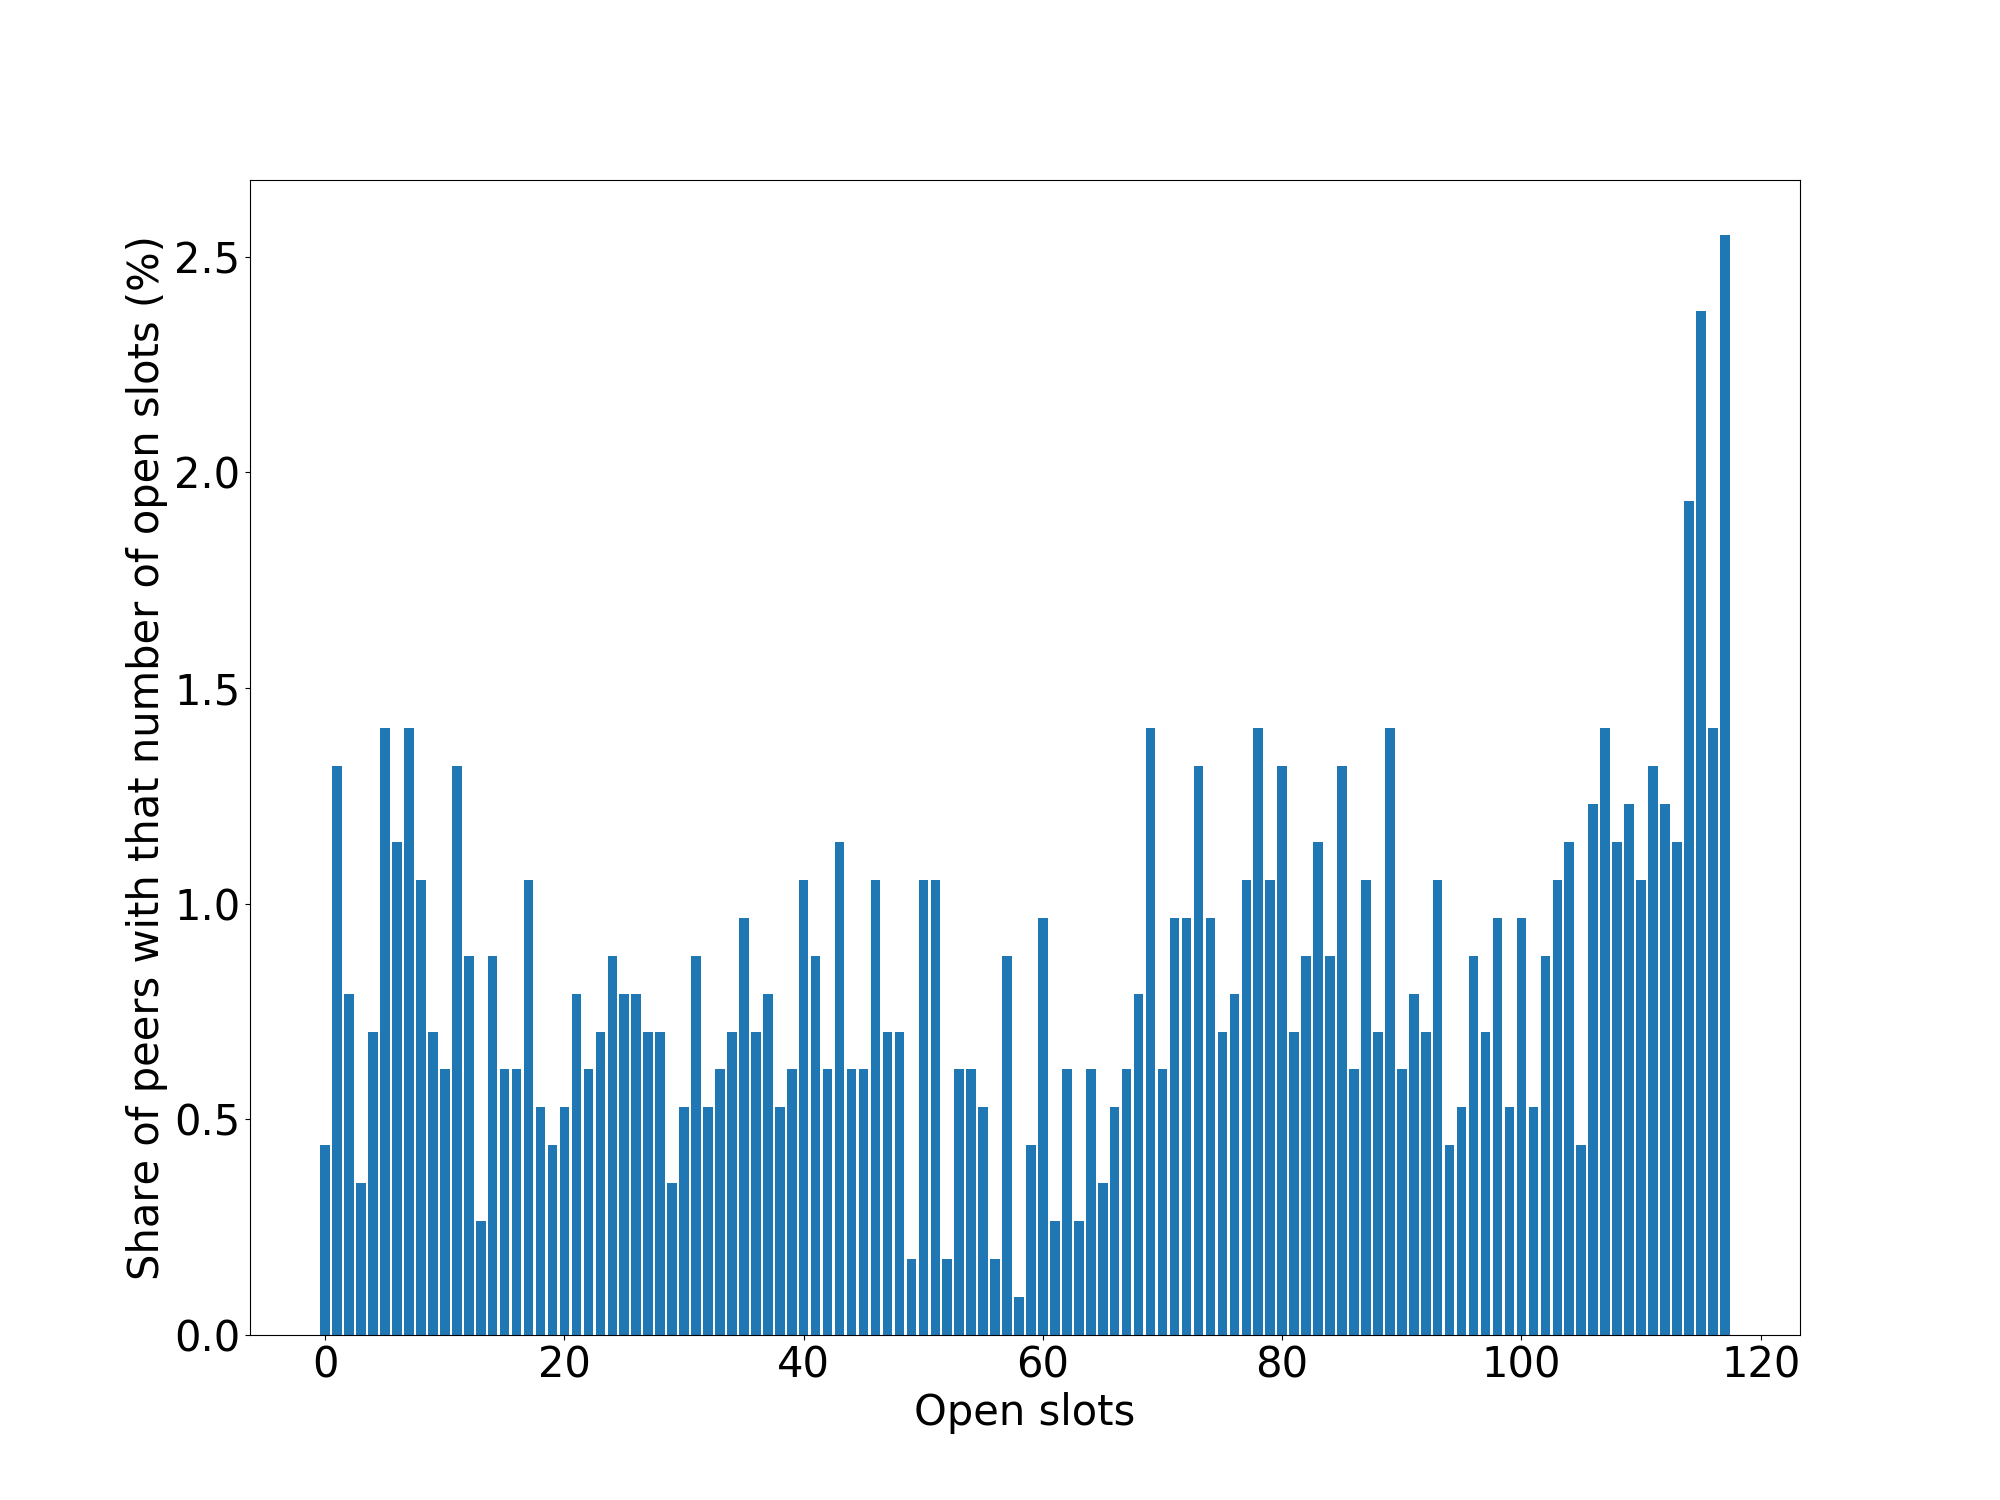
\includegraphics[width=\columnwidth]{bitcoin-testnet-1541513977-conn-max-histogram.png}
		\caption{Free connection slots for Bitcoin testnet.}
		\label{fig:free-slots-bitcoin}
	\end{minipage}\hfill
	\begin{minipage}{0.5\textwidth}
		\centering
		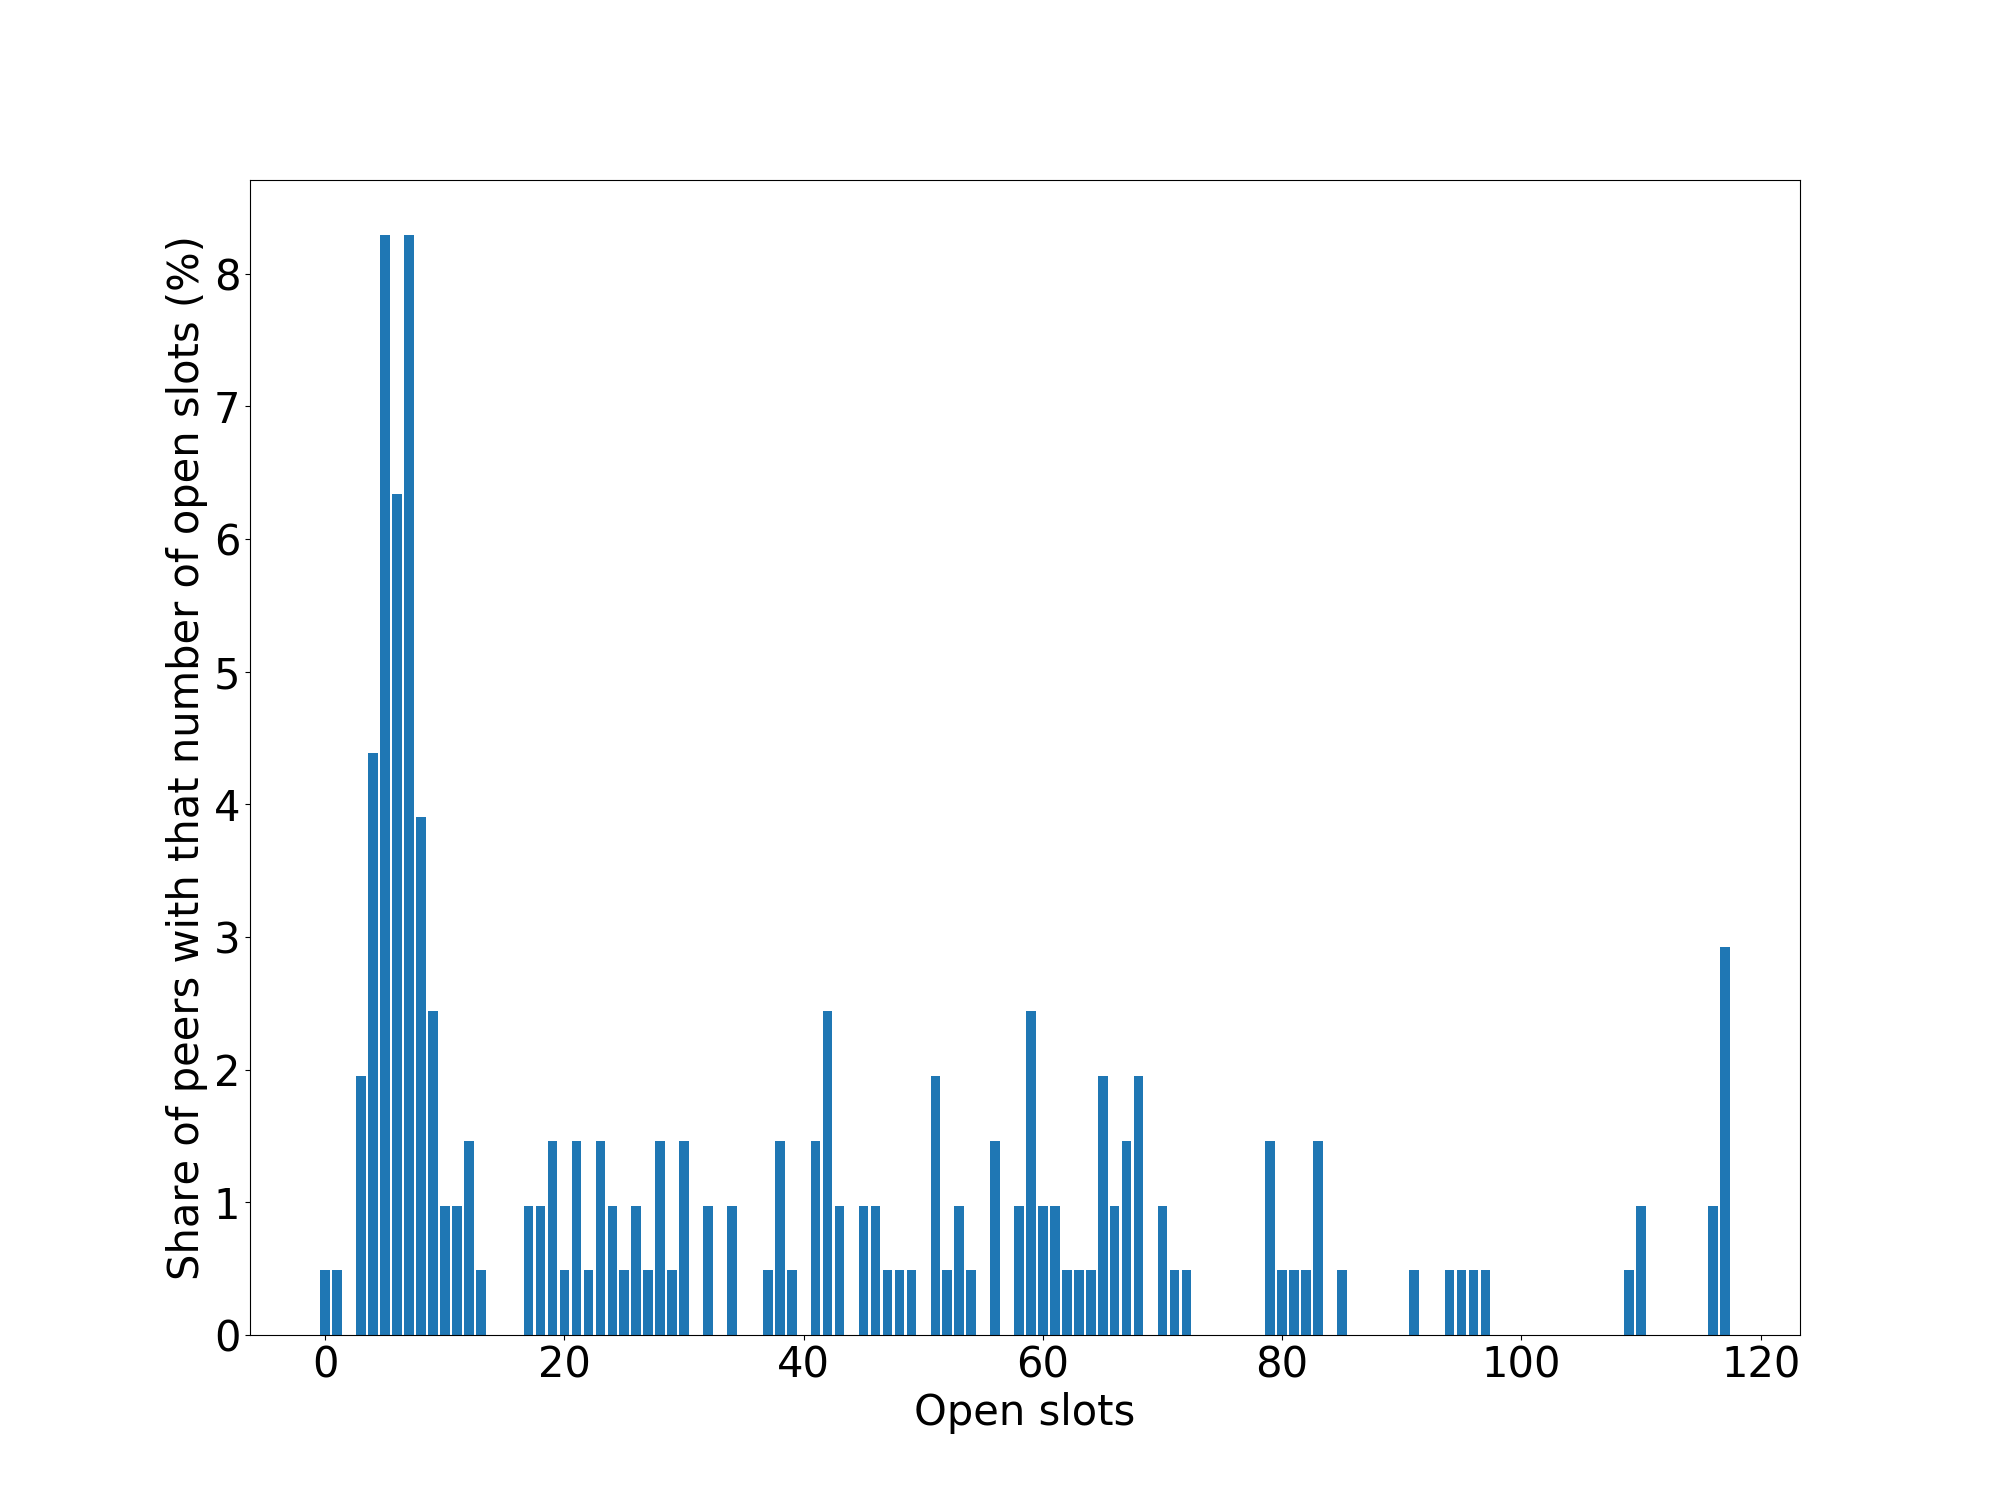
\includegraphics[width=\columnwidth]{zcash-mainnet-1541938472-conn-max-histogram.png}
		\caption{Free connection slots for Zcash mainnet.}
		\label{fig:free-slots-zcash}
	\end{minipage}\hfill
\end{figure*}


\subsubsection{Dash}

Dash is also based on the Bitcoin~Core codebase and inherits the basics of its networking protocol.
Dash uses diffusion for broadcast randomization.
The Dash networking protocol is substantially more complex compared with Bitcoin.
Dash contains $22$~new message types for masternode management~\cite{Schinzel2015}.
Masternode-related tasks include periodic pings to check whether masternodes are online, coin mixing and voting for governance proposals.
Our tool does not handle Dash-specific messages.

In our experiment, we connect to $500$~out of~$3\,065$~randomly chosen Dash nodes and ask for $30$~connection slots.
During $15$-minutes, we receive $12$~transaction inventory messages and~$396$~Dash-specific messages.

\begin{figure*}
	\centering
	\begin{minipage}{0.5\textwidth}
		\centering
		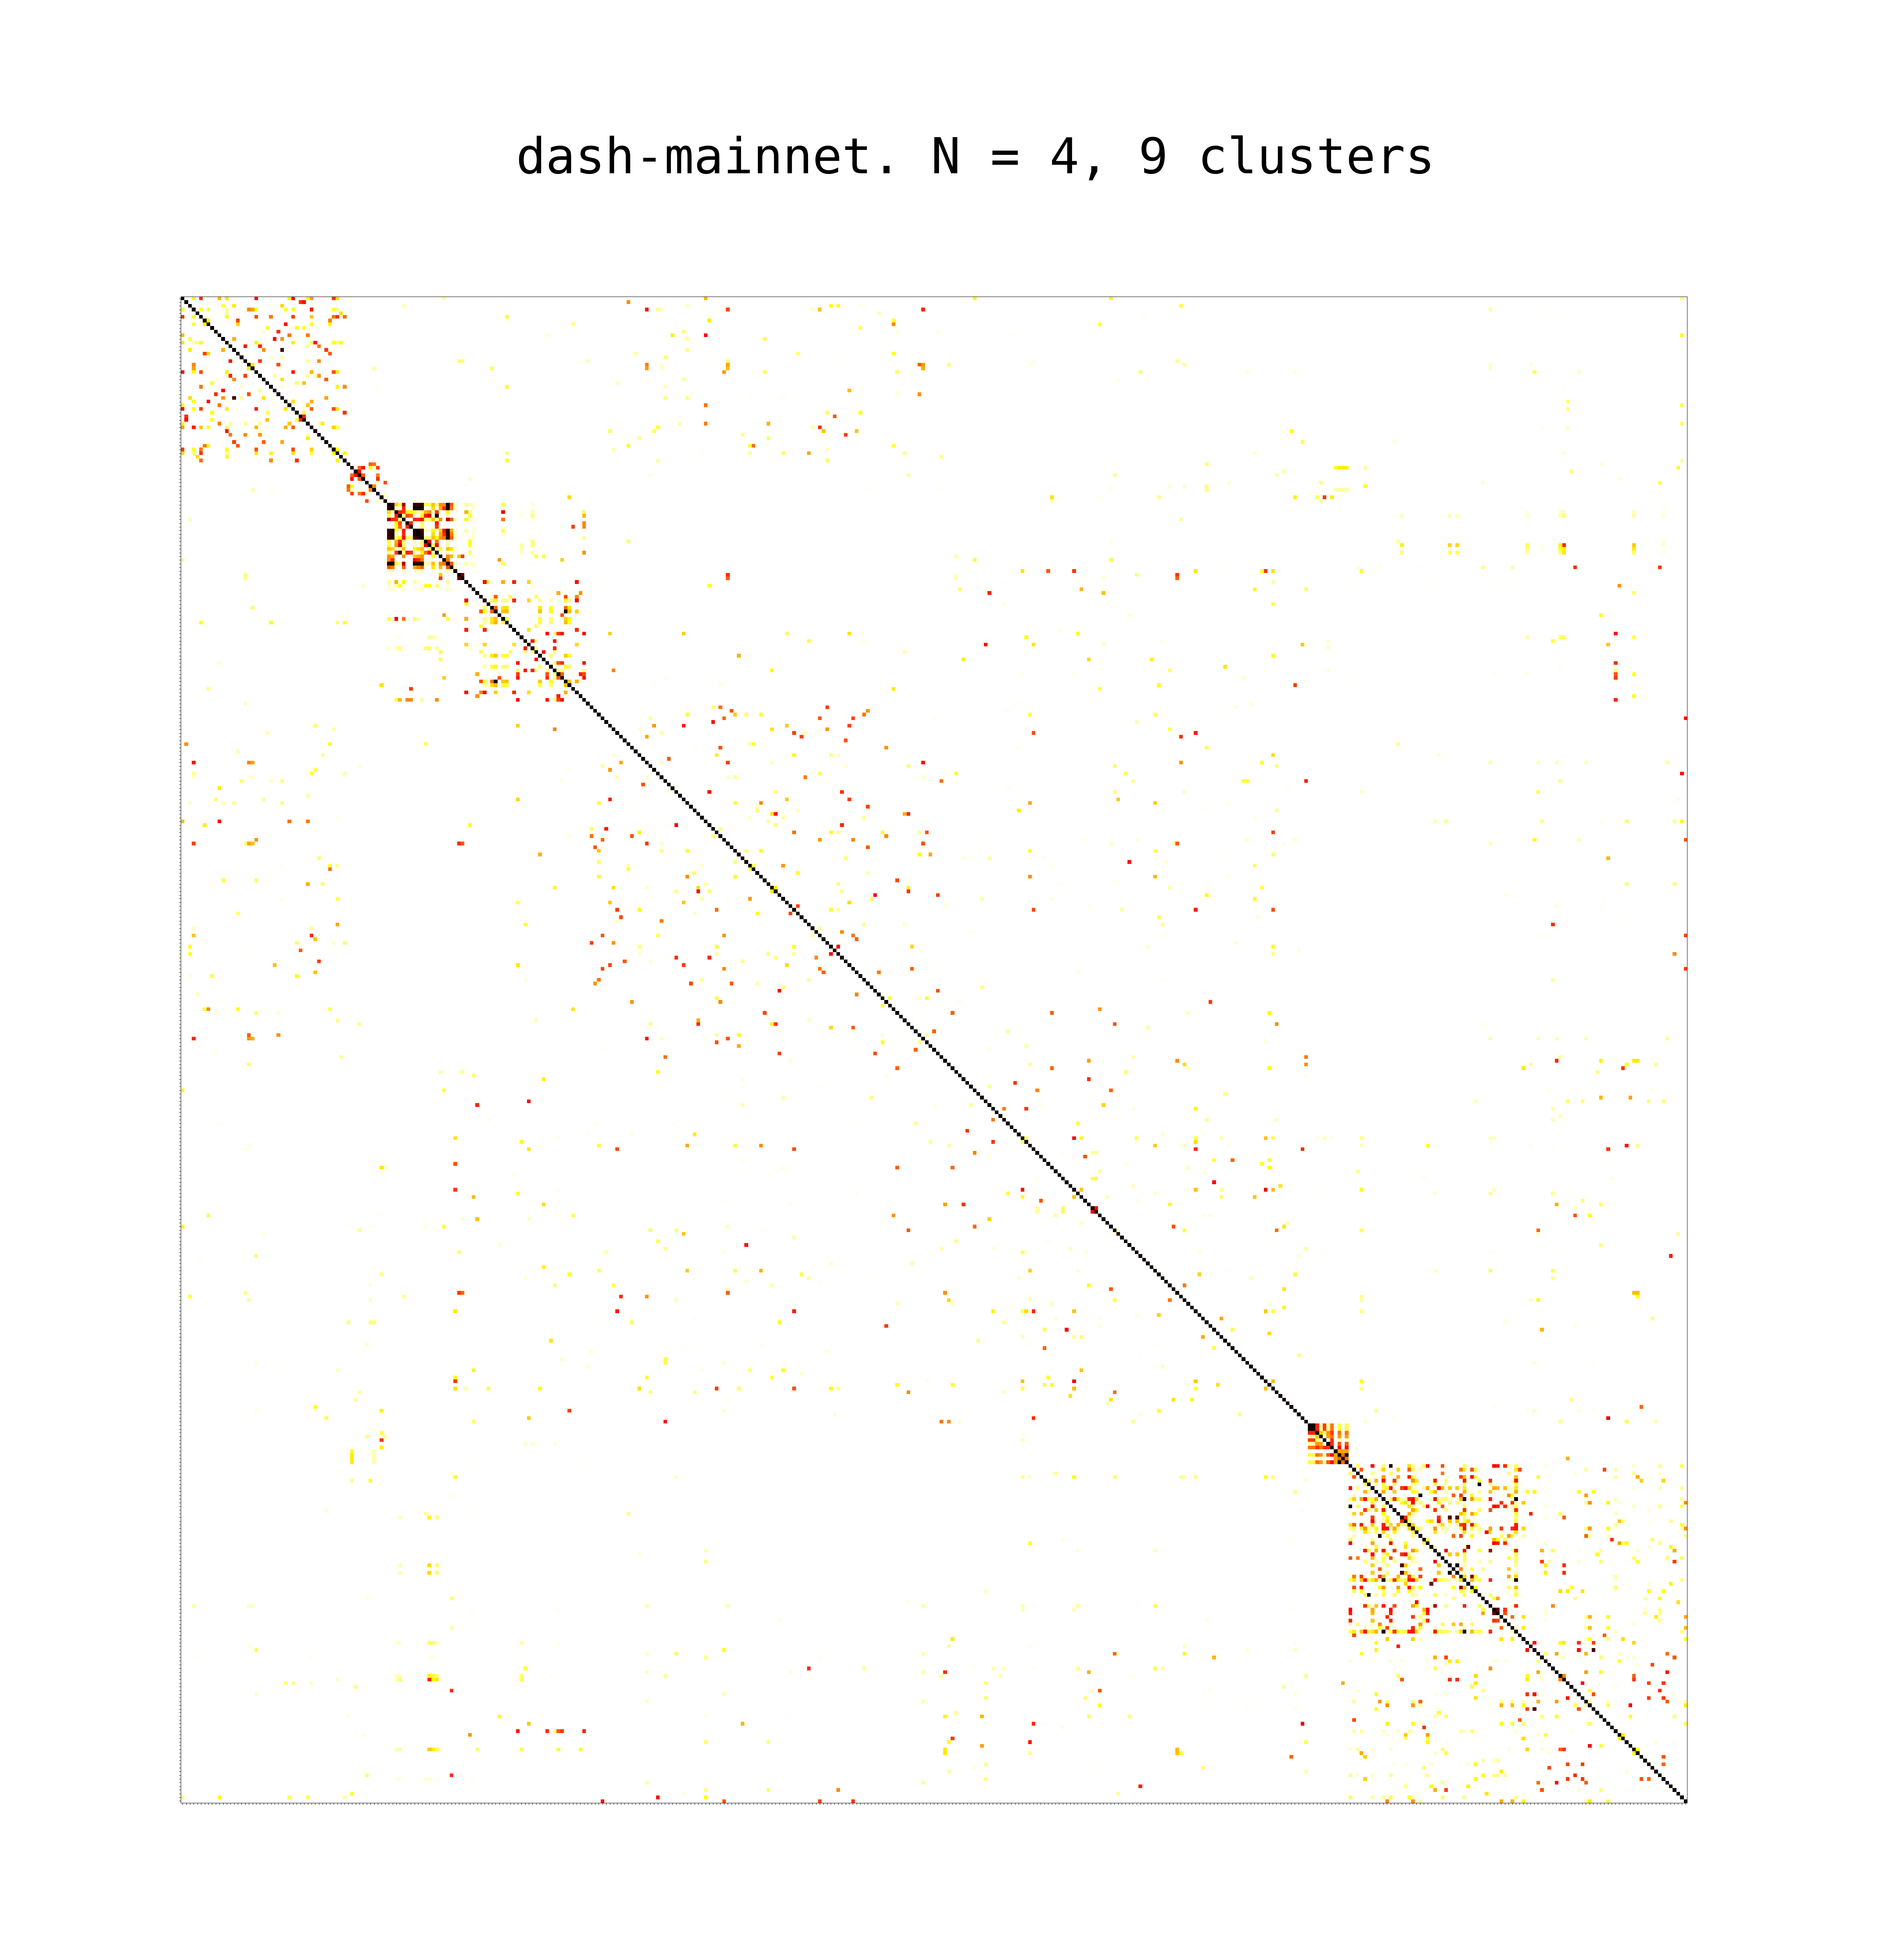
\includegraphics[width=\columnwidth]{dash-mainnet-1531510768-all.png}
		\caption{Transaction clustering for Dash (messages and transactions).}
		\label{fig:dash-all}
	\end{minipage}\hfill
	\begin{minipage}{0.5\textwidth}
		\centering
		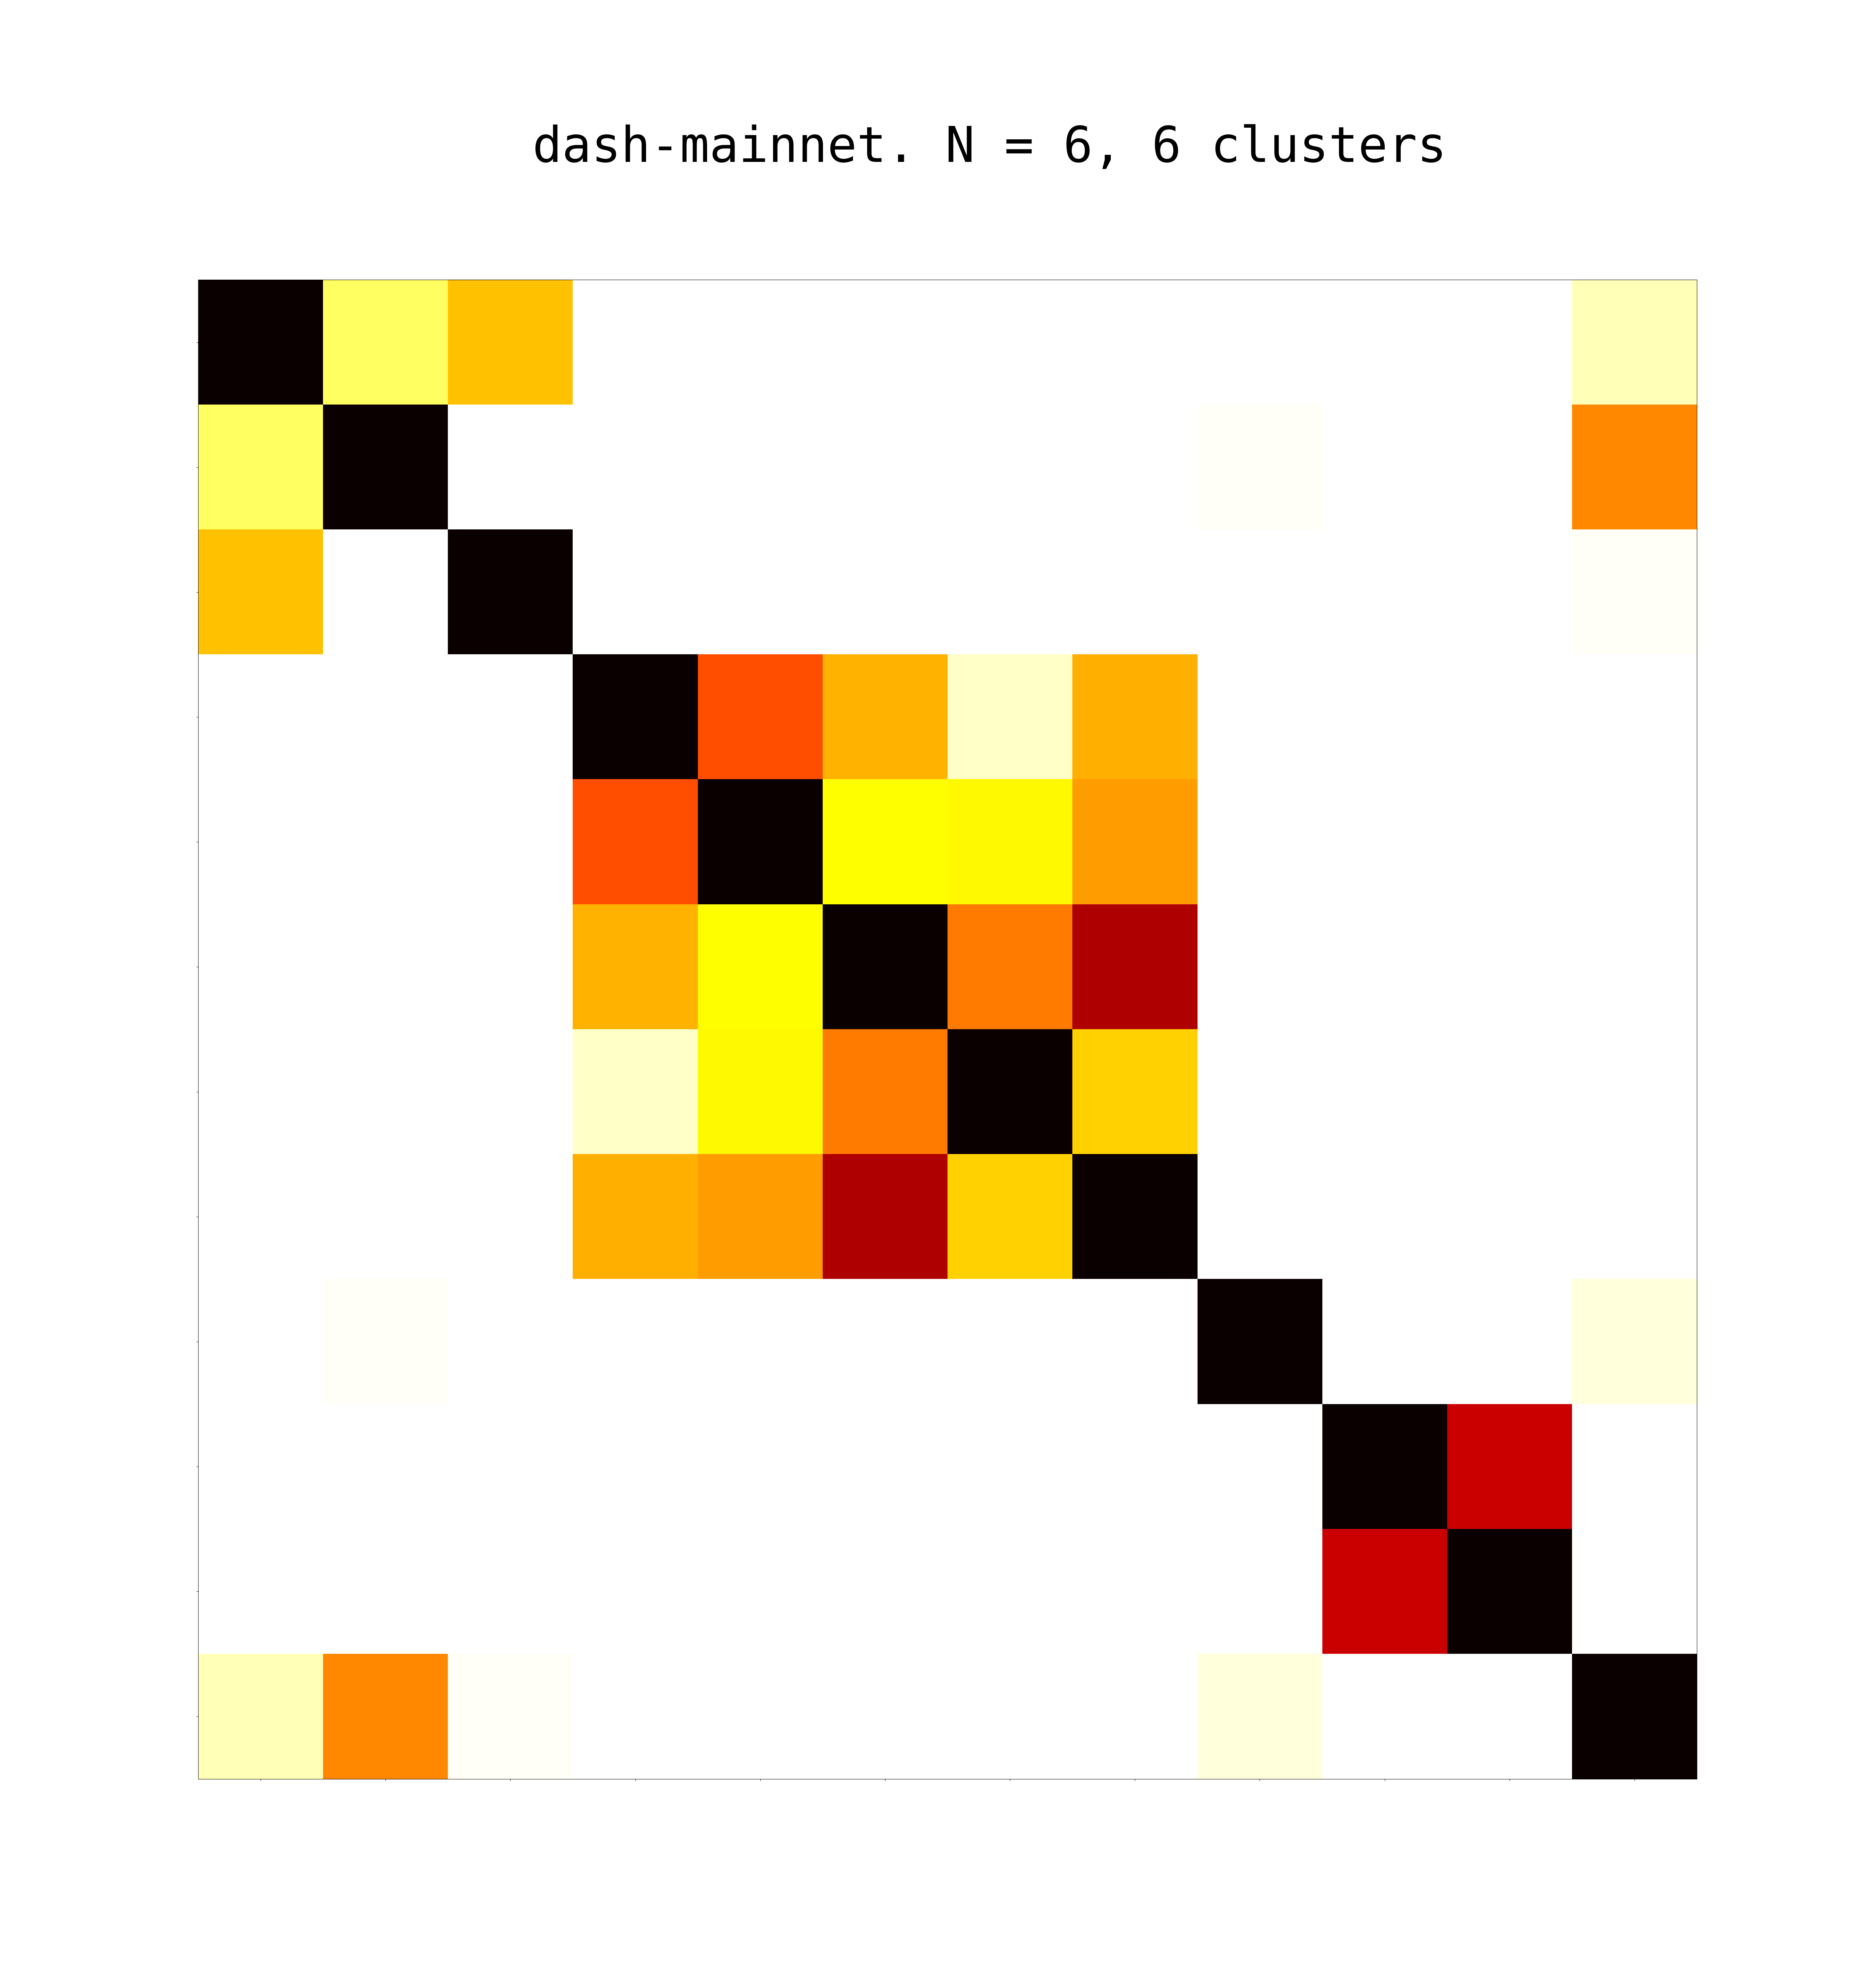
\includegraphics[width=\columnwidth]{dash-mainnet-1531510768.png}
		\caption{Transaction clustering for Dash (transactions only).}
		\label{fig:dash-tx}
	\end{minipage}\hfill
\end{figure*}

We run the clustering algorithm twice: accounting for the Dash-specific messages (Figure~\ref{fig:dash-all}), and considering only standard transaction inventory messages (Figure~\ref{fig:dash-tx}).
In both cases, we obtain clearly visible clusters.
These preliminary results show a privacy concern, especially if combined with transaction graph analysis~\cite{Kalodner2017}. 


\subsubsection{Monero}

Monero is a privacy-focused cryptocurrency not based on the Bitcoin~Core codebase.
Monero provides privacy by default: users do not have to explicitly choose the "private" option, contrary to Zcash (shielded transactions) and Dash (\textit{PrivateSend}).

The Monero community recognizes the threat of deanonymization through network analysis~\cite{user36432017, manontheinside2016, expez2016, Cameron2016}.
This has motivated the integration of Dandelion++ networking protocol in 2020~\cite{ErCiccione2020} (see Section~\ref{sec:Dandelion}).
Moreover, the Kovri project~\cite{Kovri} aims to add an I2P router into Monero.
As of the time of our experiments (mid-2018), Monero uses no broadcast randomization.

Monero does not allow creating and spending a transaction output in the same block.
A new output appears as "locked" until the transaction that creates it receives $10$~confirmations ($20$~minutes at the target block time of~$2$~minutes)~\cite{dpzz2017}.
Though this is a wallet-level and not a protocol-level restriction, the official desktop wallet and Monerujo, a popular Monero wallet for Android, enforce it.
Therefore, the scenario of our earlier experiments is somewhat unrealistic.
For example, to issue $20$~transactions within a $20$~minute period, a user must have $20$~"unlocked" transaction outputs (each takes $20$~minutes to create).

We conduct an experiment on Monero without issuing transactions.
This experiment aims to detect a block-diagonal structure in the correlation matrix derived from real-world transactions.
We connect to $200$~nodes and receive $124$~transactions in a $38$~minute window (Figure~\ref{fig:monero}).

\begin{figure}[!t]
	\centering
	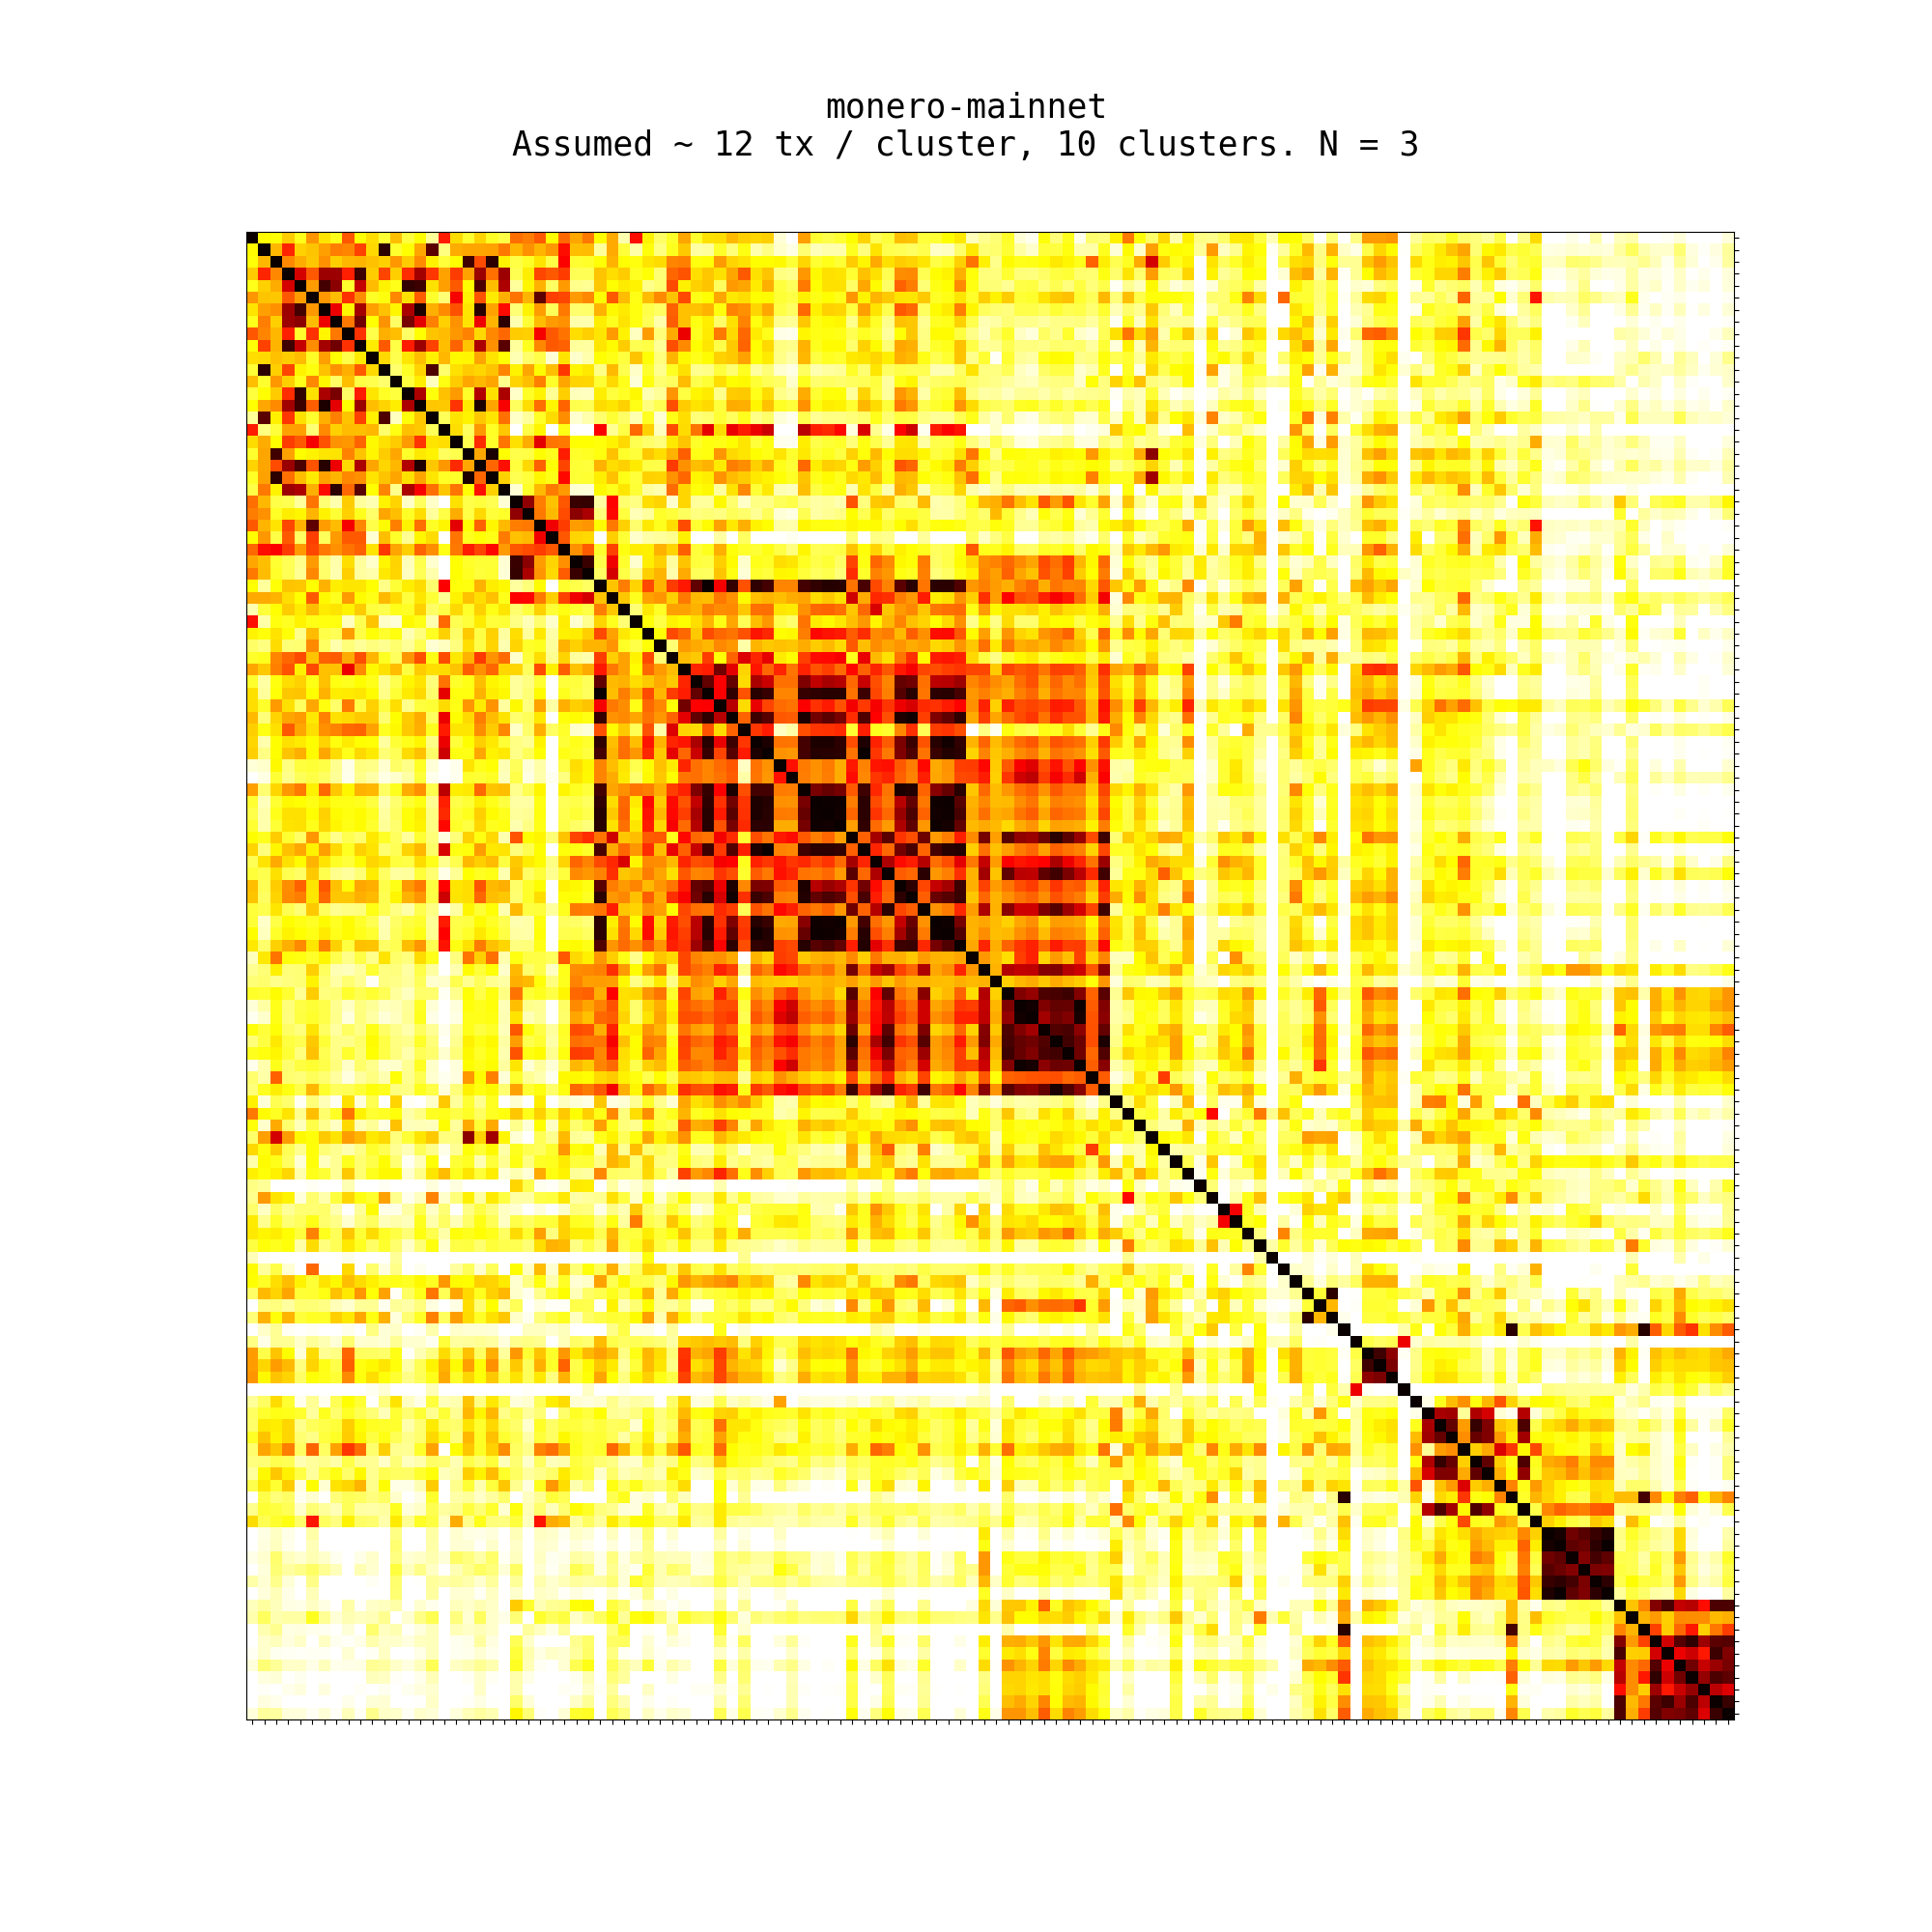
\includegraphics[width=0.5\columnwidth]{monero-mainnet-005-fig-correlations-012-txcl-003-N-Rand-best.png}
	\caption{Transaction clustering for Monero.}
	\label{fig:monero}
\end{figure}

We explain a less clear picture compared to Bitcoin testnet as follows.
First, we connect to only~$200$ out of $1\,700$--$1\,800$ nodes (as of the time of the experiment~\cite{MoneroHash}).
Second, Monero does not use the three-step transaction propagation (\texttt{inv} -- \texttt{getdata} -- \texttt{tx}), which may have opposite effects on clustering quality.
On the one hand, relaying a transaction unconditionally to all neighbors increases the probability that we receive a new transaction from a node other than the source of one of its entry nodes.
On the other hand, this broadcast type may provide a near-perfect insight into transaction sources, if the attacker connects to all or nearly all nodes.
Third, \texttt{monerod} connects to nodes slower than \texttt{bcclient}, which impedes data collection.
In our experiment, while trying to connect to $200$~nodes, we obtain $150$~connections after approximately $2$~hours, $175$~connections after $3$~hours, $200$~connections after nearly $8$~hours.

Monero uses hard-coded DNS seeds and seed IP addresses for bootstrapping (see Chapter~\ref{sec:BitcoinP2PProtocol}).
As of July~2018, all DNS seeds fail to resolve.
The official client falls back to seed IP addresses.


\subsection{Results for mobile wallets}

We perform analogous experiments on Bitcoin (testnet and mainnet) and Zcash issuing transactions from selected mobile wallets for Android.
Most mobile wallets connect to the P2P network via a trusted server maintained by the wallet's developers.
We refer to wallets that connect to the P2P network directly as \textit{P2P wallets}.
Most P2P wallets rely on the BitcoinJ library for networking.
None of them uses broadcast randomization.
Unlike Bitcoin~Core, BitcoinJ sends \texttt{tx} unconditionally\footnote{Note that in this case, a full node receiving a \texttt{tx} message from an SPV node can be sure that the transaction originated at that SPV node, whereas receiving an \texttt{inv} announcement from a full node may also be a re-broadcast. This demonstrates the privacy enhancement of exclusively connecting to a trusted node for SPV.}.
The BitcoinJ developers acknowledge that the three-step \texttt{inv} -- \texttt{getdata} -- \texttt{tx} exchange in Bitcoin~Core improves privacy, but argue that since SPV nodes have a weaker privacy model, the three-step broadcast would only decrease efficiency.

We choose a diverse selection of mobile wallets for our experiments: Bitcoin-only and multi-coin, with centralized and P2P networking.
We perform experiments on the Bitcoin testnet (Bitcoin wallet), the Bitcoin mainnet (Bitcoin wallet, BRD, Coinomi, Mycelium), and Zcash (Coinomi).
Bitcoin wallet and BRD\footnote{Bitcoin wallet and BRD are the two most popular Bitcoin clients~\cite{Wang2017}.} use P2P broadcast.
Coinomi and Mycelium use centralized broadcast.
For wallets with centralized broadcast, we only issue one set of transactions, using it as a "label" for a presumed wallet cluster.
If our transactions form a visible cluster, we inspect the IP addresses of nodes among the first ones to broadcast them.
Thus we infer the IP addresses of nodes likely to be used for transaction broadcasts for this wallet.
This information allows us to associate transactions in the network with popular wallets later.

\begin{figure}
	\centering
	\begin{subfigure}{.5\textwidth}
		\centering
		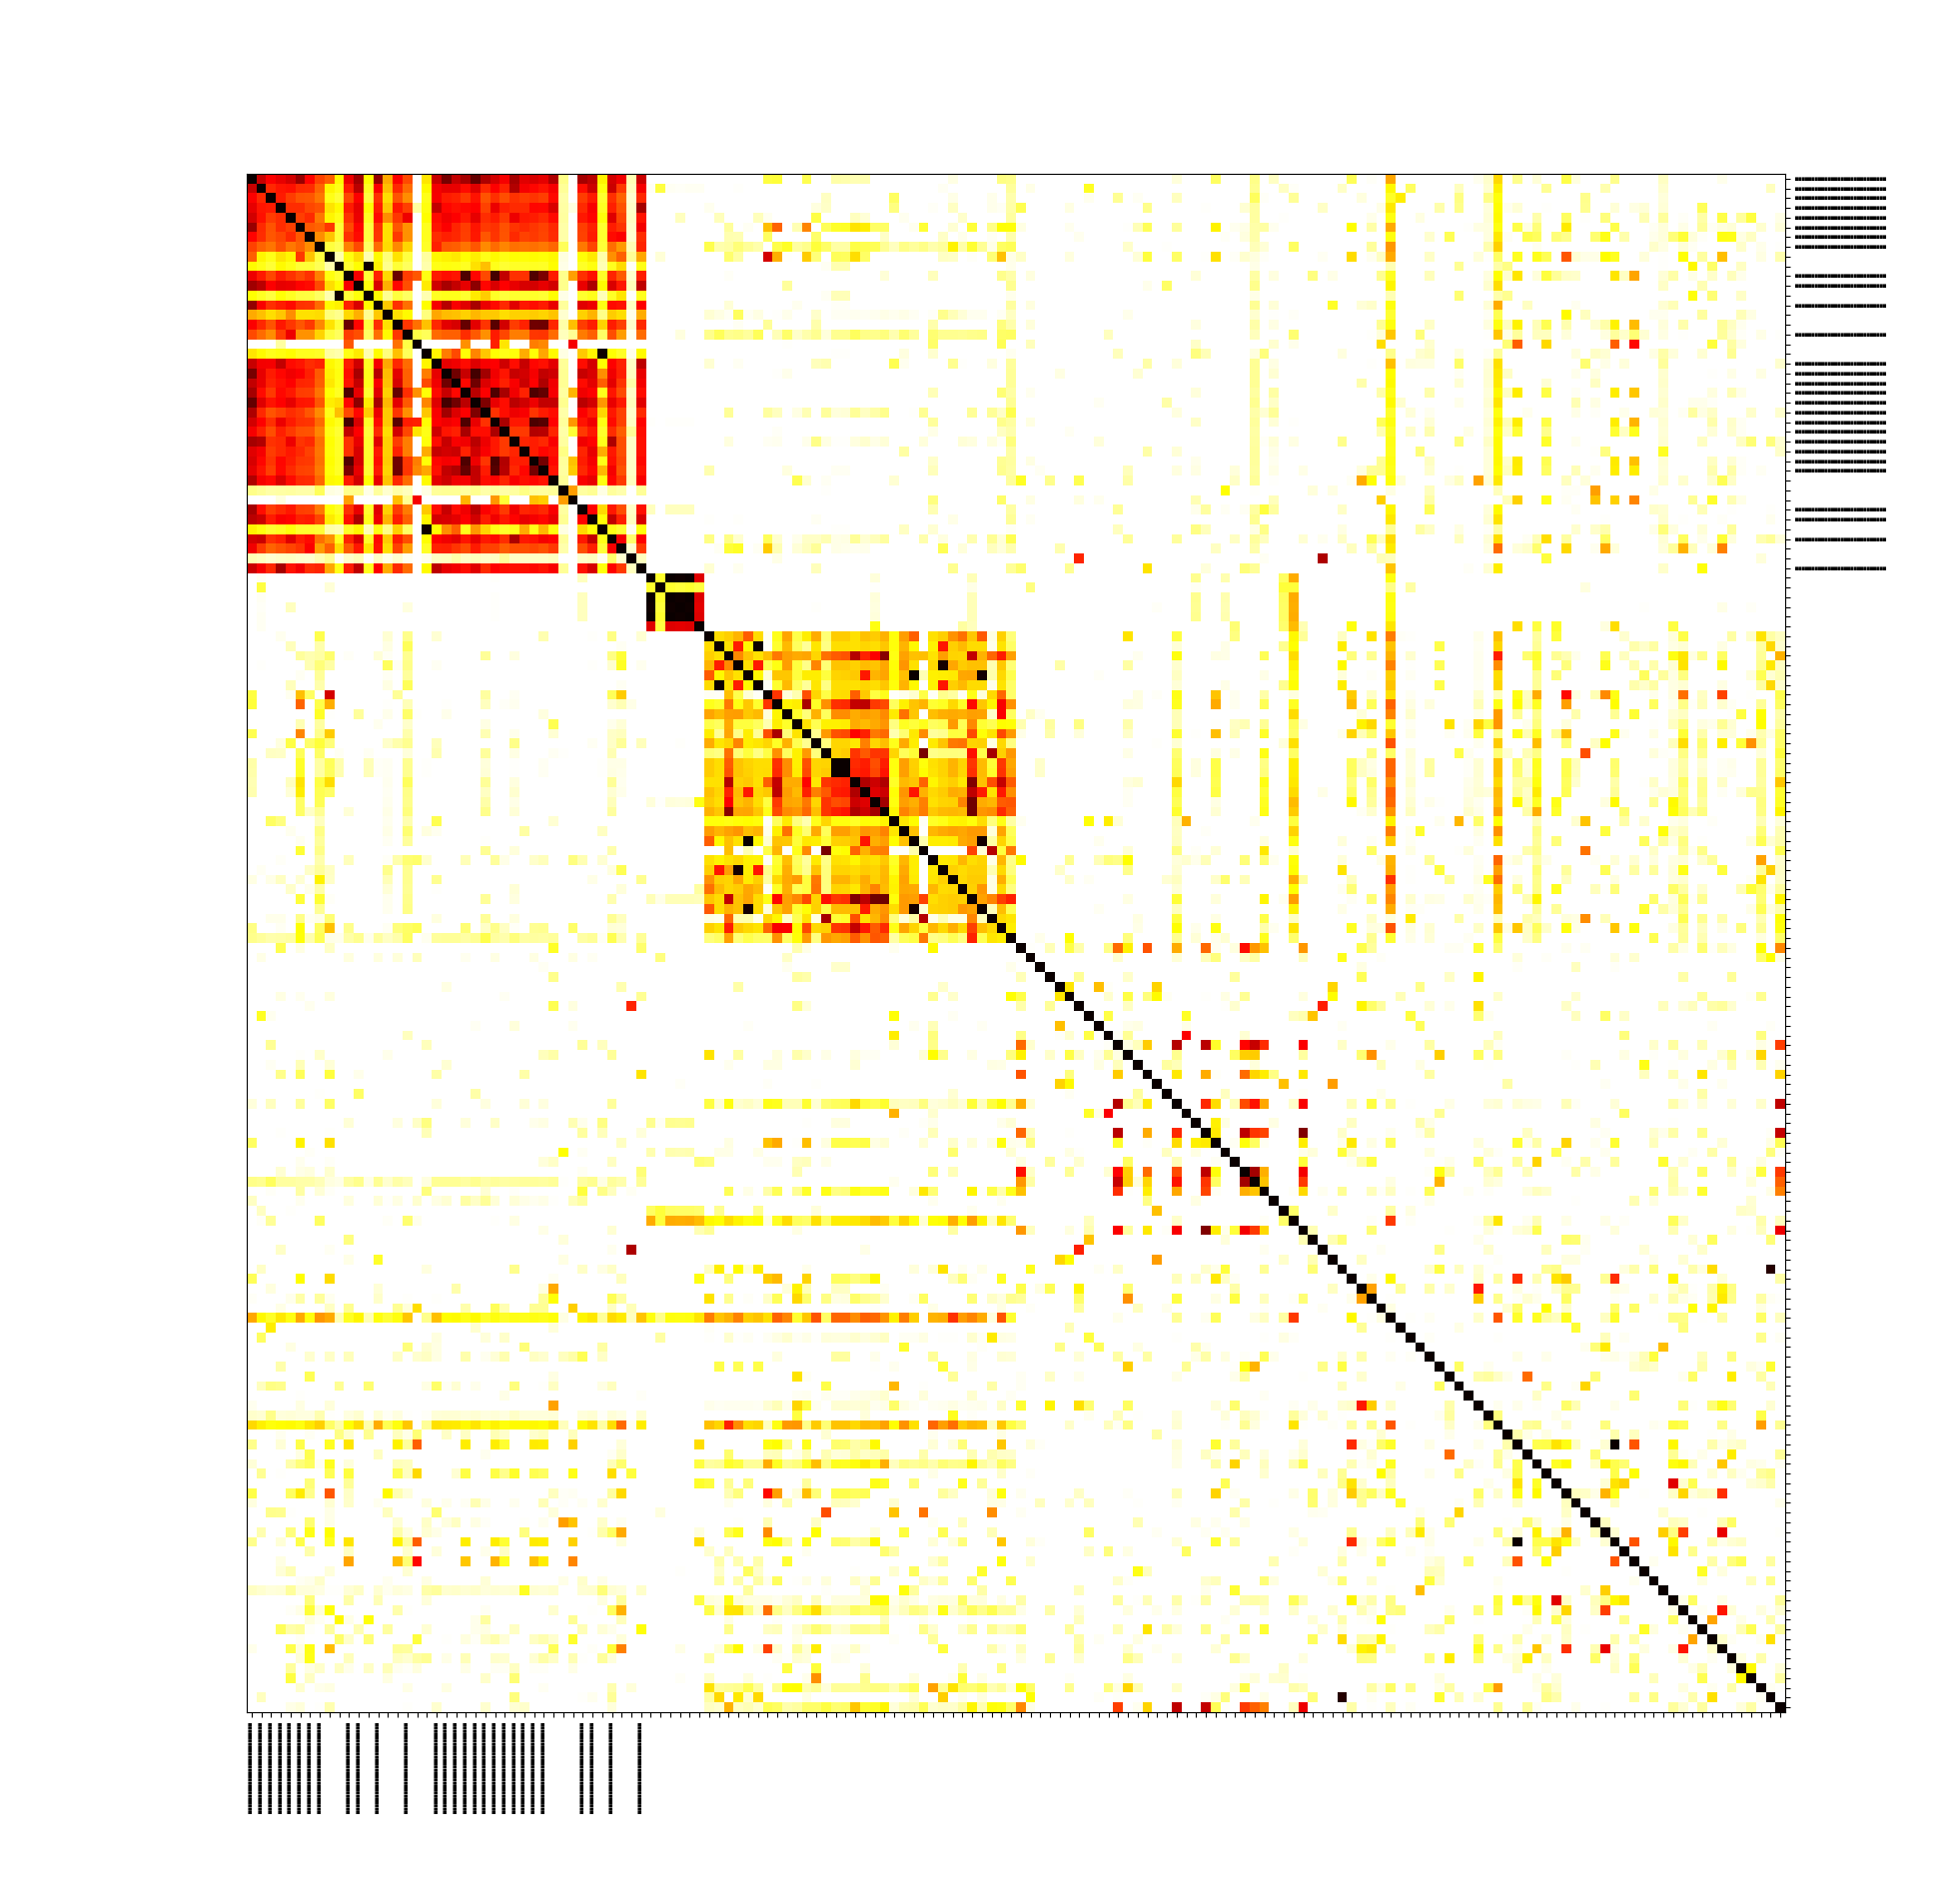
\includegraphics[width=\columnwidth]{bitcoin-testnet-1542895555-fig-corr-032-txcl-005-N-Rand.png}
		\caption{Bitcoin testnet, Mycelium.}
	\end{subfigure}%
	\begin{subfigure}{.5\textwidth}
		\centering
		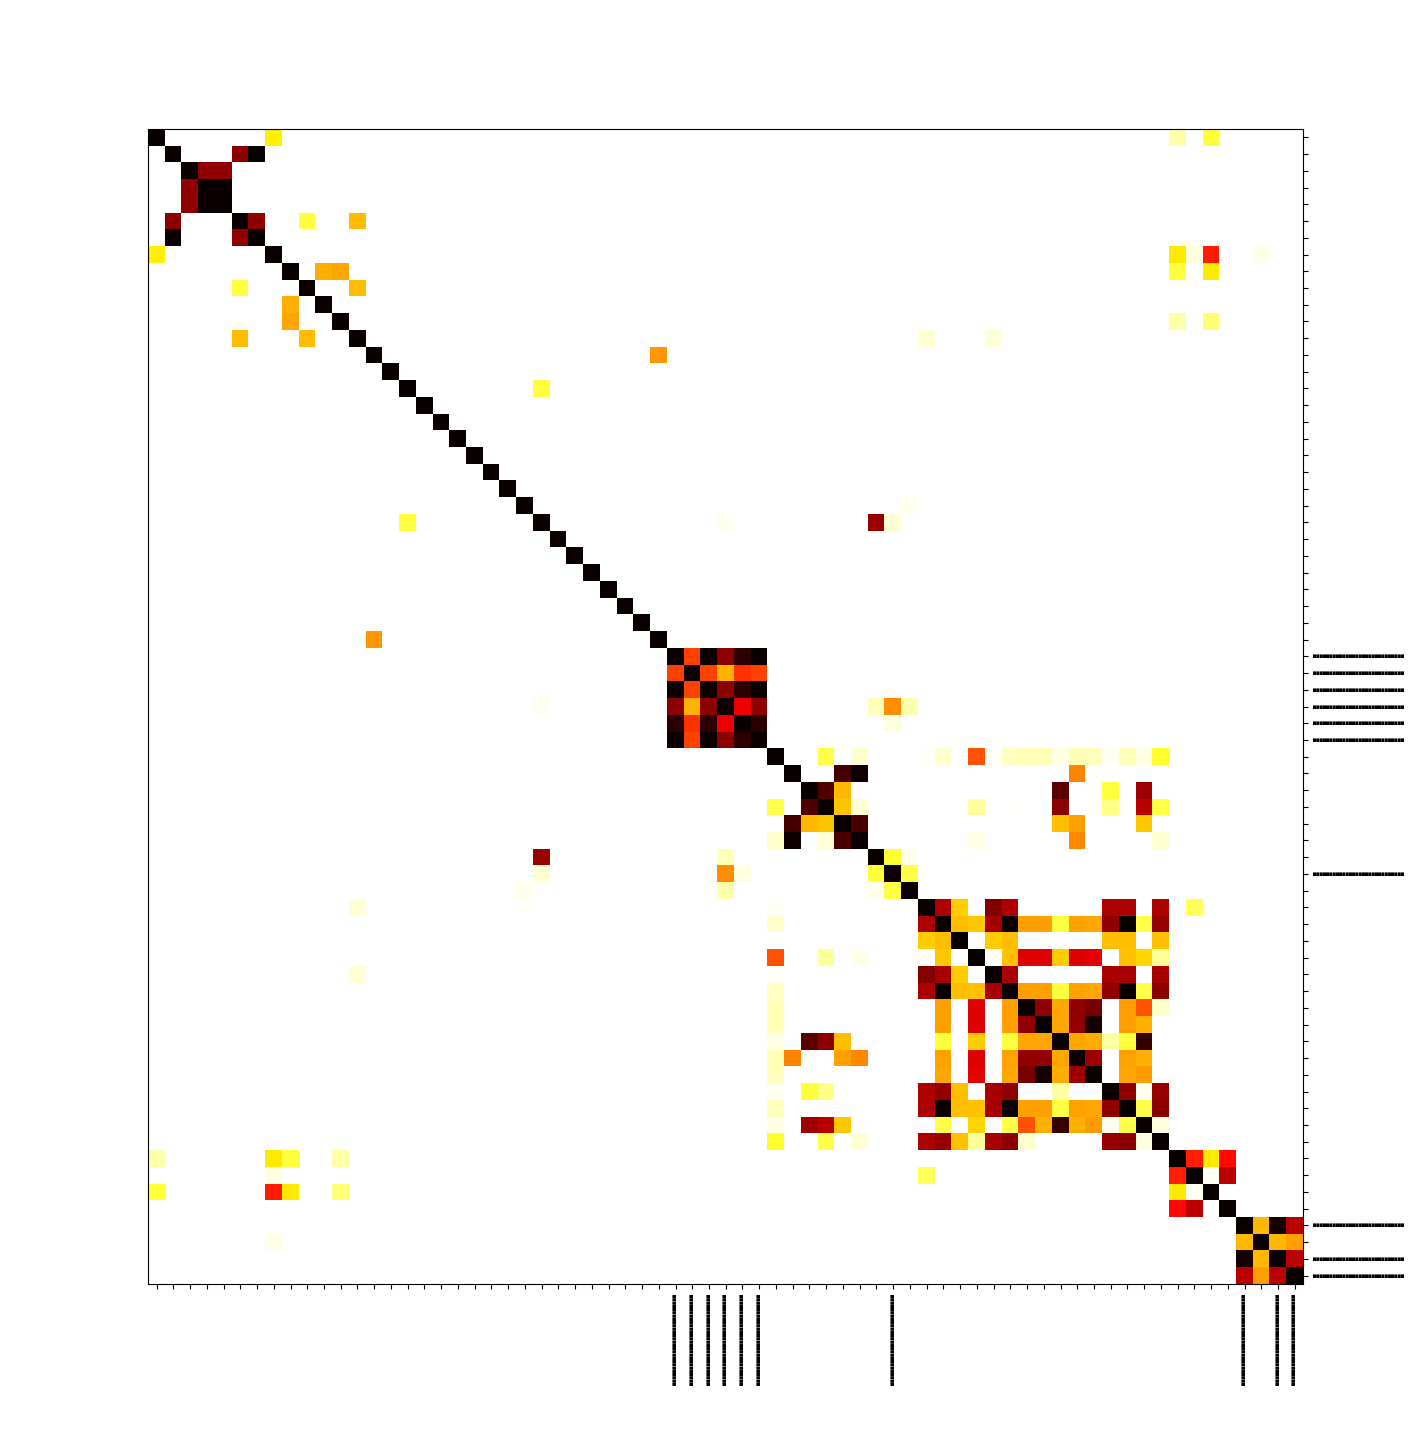
\includegraphics[width=\columnwidth]{bitcoin-testnet-1537202356-fig-corr-008-txcl-003-N-Rand.png}
		\caption{Bitcoin testnet, Bitcoin wallet.}
	\end{subfigure}
	\begin{subfigure}{.5\textwidth}
		\centering
		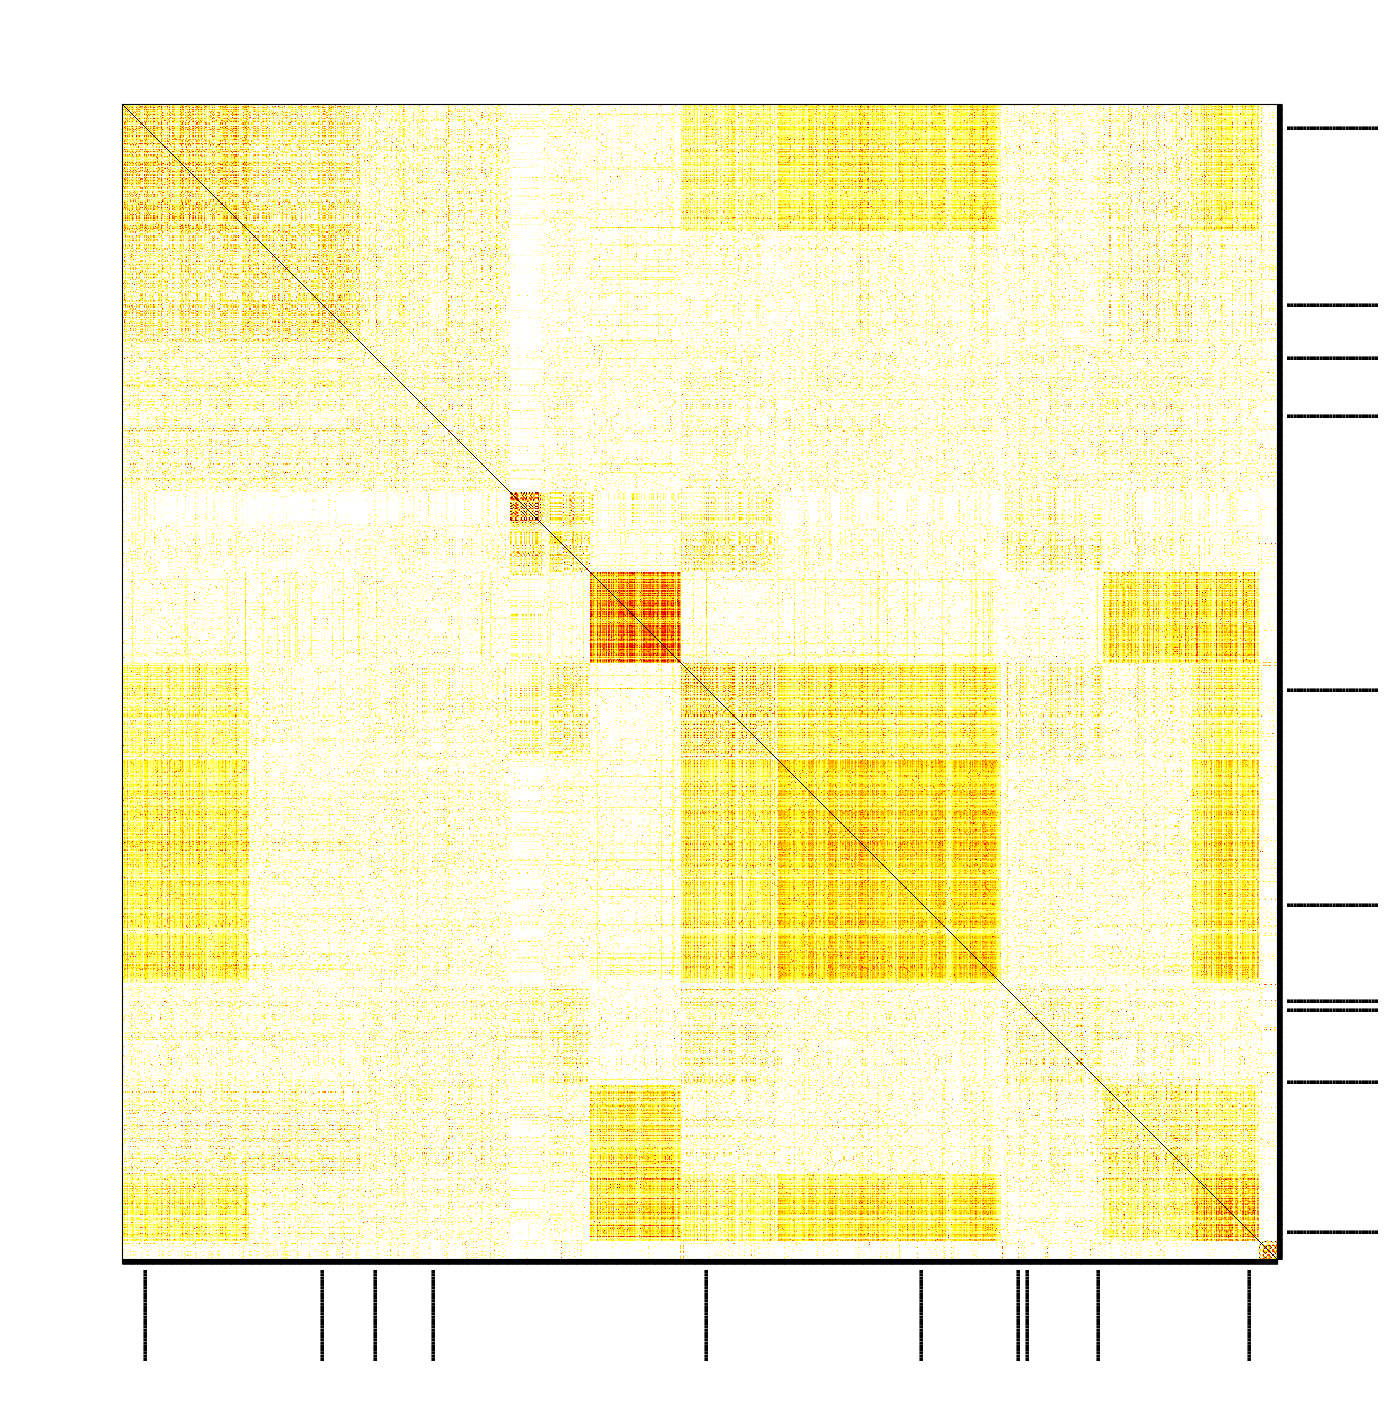
\includegraphics[width=\columnwidth]{bitcoin-mainnet-1537365306-fig-corr-202-txcl-007-N-Rand.png}
		\caption{Bitcoin mainnet, Bitcoin wallet.}
	\end{subfigure}%
	\begin{subfigure}{.5\textwidth}
		\centering
		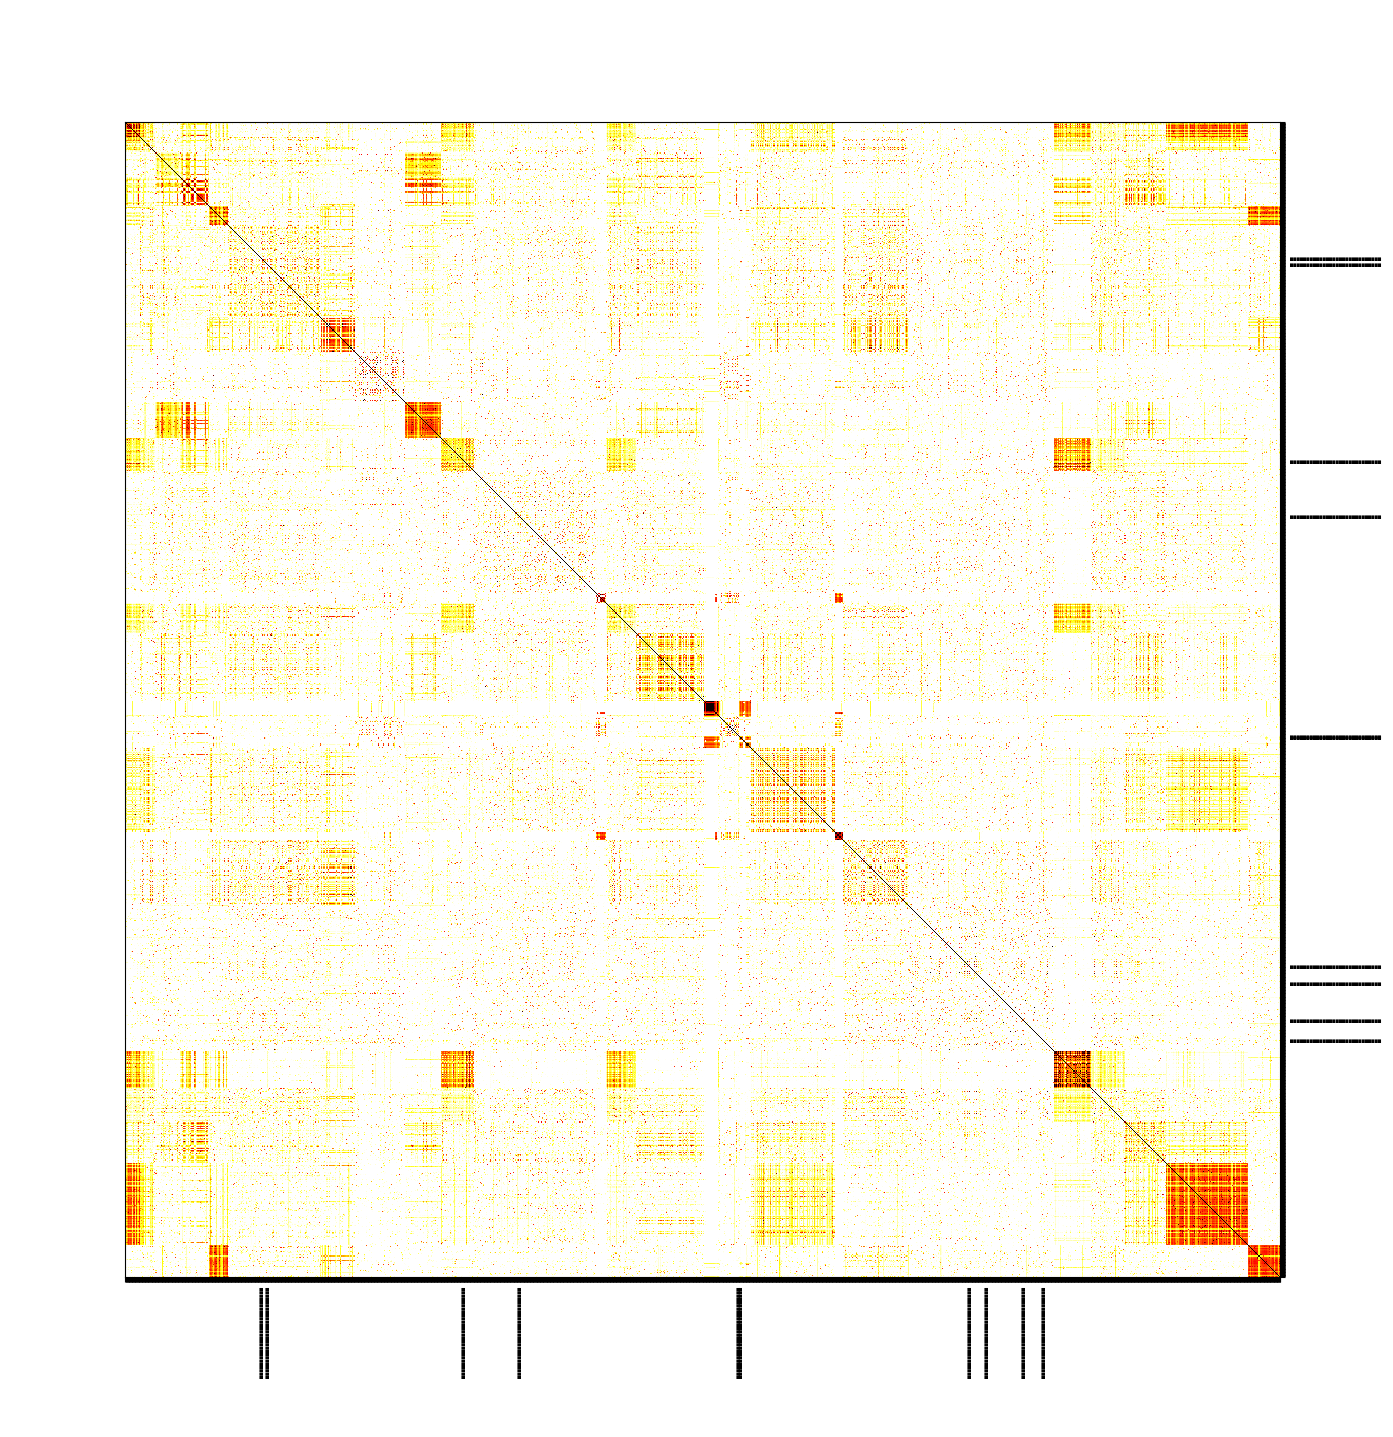
\includegraphics[width=\columnwidth]{bitcoin-mainnet-1537377559-fig-corr-102-txcl-004-N-Rand.png}
		\caption{Bitcoin mainnet, BRD.}
	\end{subfigure}
	\begin{subfigure}{.5\textwidth}
		\centering
		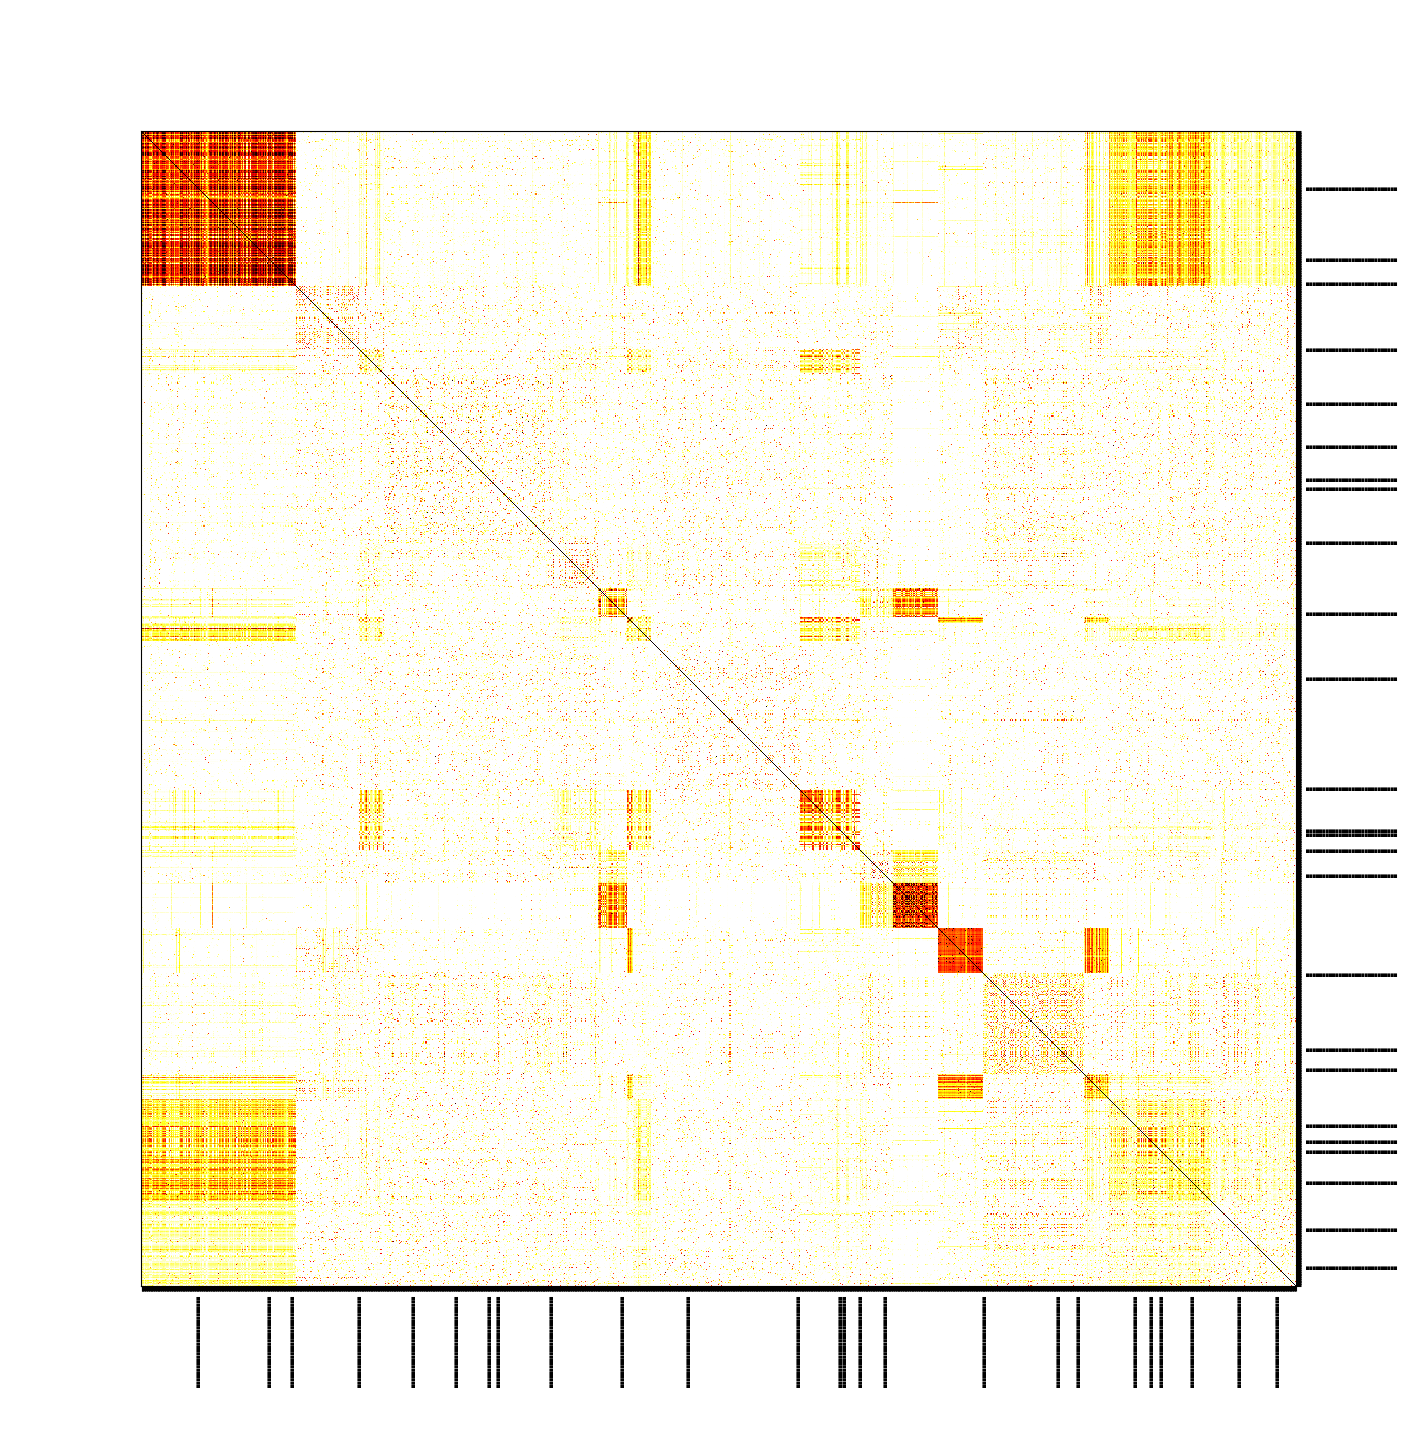
\includegraphics[width=\columnwidth]{bitcoin-mainnet-1537951300-fig-corr-100-txcl-004-N-Rand.png}
		\caption{Bitcoin mainnet, Coinomi.}
	\end{subfigure}%
	\begin{subfigure}{.5\textwidth}
		\centering
		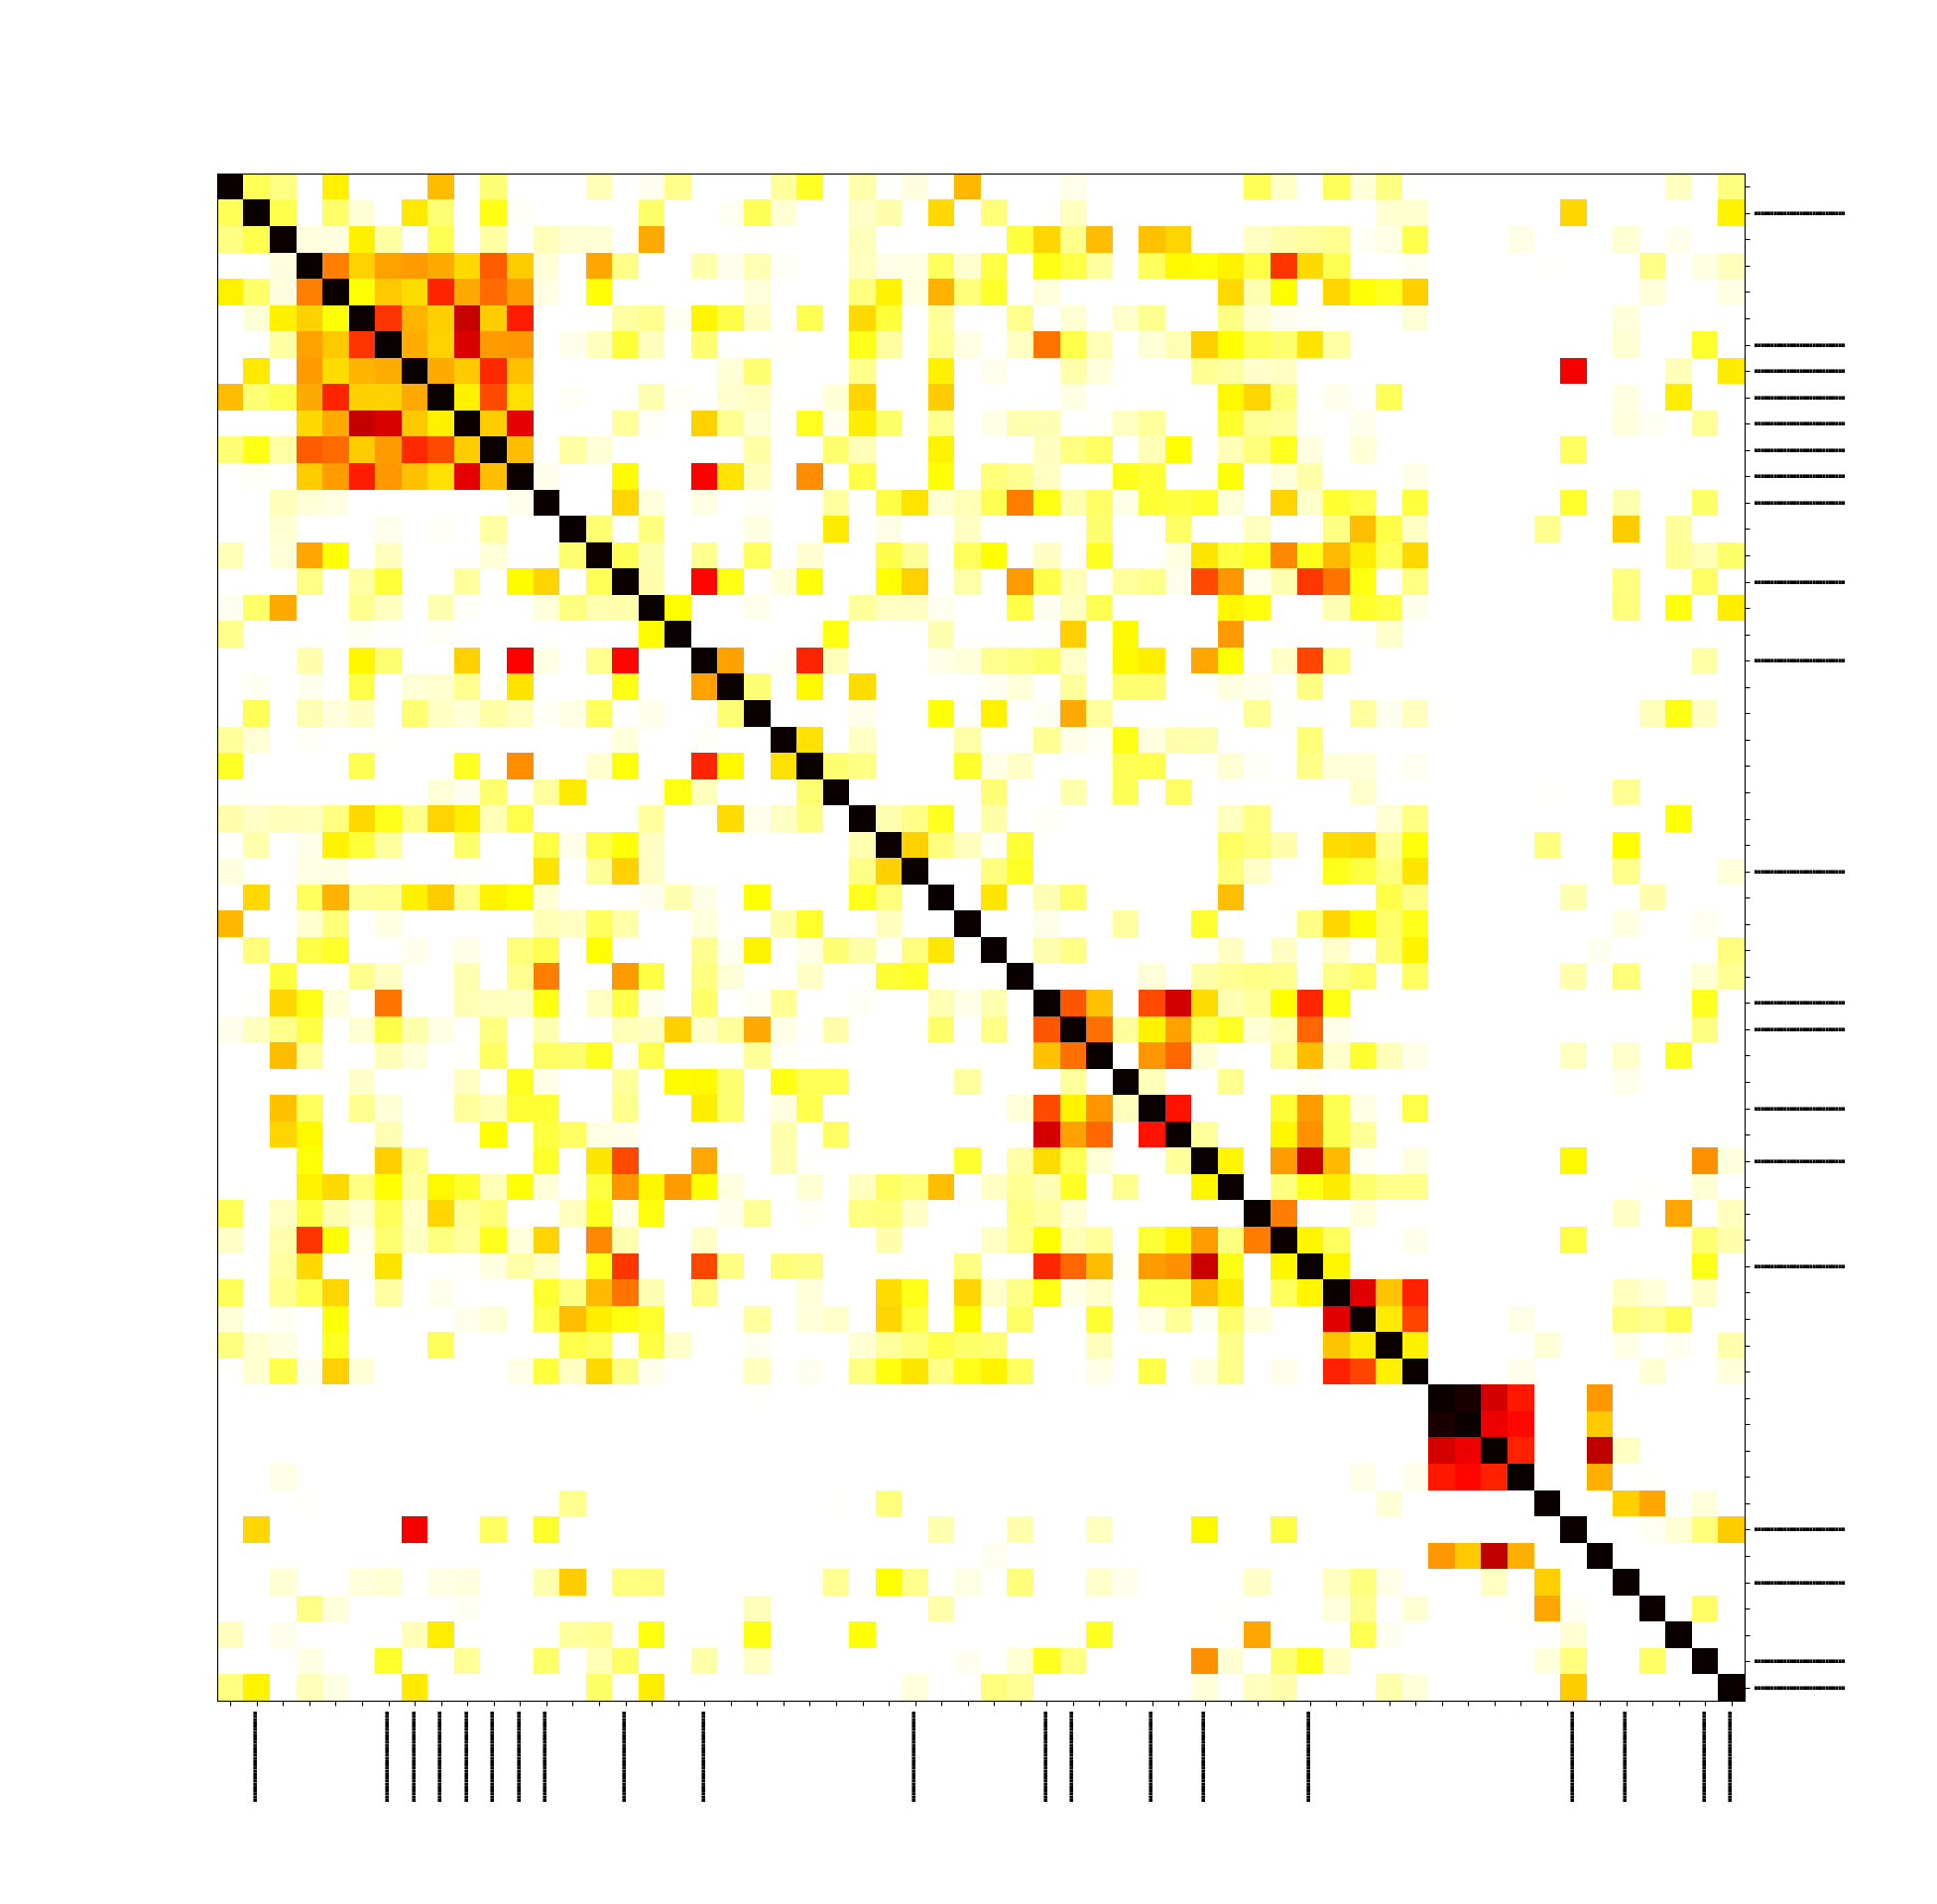
\includegraphics[width=\columnwidth]{zcash-mainnet-1543922496-fig-corr-005-txcl-003-N-Rand.png}
		\caption{Zcash, Coinomi.}
	\end{subfigure}
	\caption{Transaction clustering for mobile wallets.}
	\label{fig:clustering-all}
\end{figure}

As expected, the correlation matrices exhibit a block-diagonal structure (Figure~\ref{fig:clustering-all}).
The clusters are clearly visible for the Bitcoin wallet on testnet, for which we obtained the anonymity degree of~$0.5089$.
The adjusted anonymity degree for the Bitcoin mainnet is $0.8646$~for Bitcoin wallet, $0.8413$~for BRD, and~$0.9117$~for Coinomi.
Similar to the results with a desktop node as a transaction source, the picture for the Bitcoin mainnet is much less clear because of more transactions and nodes overall and a smaller number of connections that we establish.


\subsubsection*{Estimating the IP addresses of wallet's nodes}

Apart from clustering transactions, an adversary might be interested in obtaining the IP address of the nodes that a centralized wallet uses for transaction broadcast.
The IP address of a centralized wallet's node may not necessarily be secret.
Still, linking Bitcoin transactions with IP addresses may reveal which wallet a victim is using.
The adversary can later leverage this information for social engineering attacks.

We test this attack scenario in two experiments (Figure~\ref{fig:clustering-all}).
In the first experiment, we consider the Bitcoin testnet and Mycelium wallet.
The Mycelium transactions exhibit a clearly visible cluster: they are quickly announced from the same two IP addresses.
The time difference between these announcements is in single milliseconds.
Other nodes re-broadcast then only after tens or hundreds of milliseconds.
According to IP geolocation services, the two nodes are located in Germany (\texttt{2a01:4f9:2b:4ca::2}) and in Helsinki, Finland (\texttt{95.216.68.181}).
A reverse DNS lookup service \url{robtex.com} suggests that one of these IP addresses corresponds to a URL~\url{electrumx-b.mycelium.com}.
Both IP addresses belong to Hetzner (a cloud provider) and host Bitcoin nodes with a latency of~$25$~ms~\cite{Bitnodes}.
We estimate that each of these nodes offers more than $700$~connection slots in a separate experiment.
The second experiment considers Zcash and Coinomi wallet.
Though the Coinomi transactions do not form a clear cluster, we observe that some of them (in the second cluster) are quickly announced from the same IP (\texttt{5.79.123.194}), which, we assume, is one of the Coinomi's nodes.


\section{Attack cost estimation}

We now estimate the resources required for a full-scale attack on the Bitcoin mainnet.
The Bitcoin mainnet consists of approximately $10\,000$~nodes reachable at any given time~\cite{Bitnodes}.
Bitcoin nodes to provide $43$~connections slots on average (measured on $1\,000$~random nodes).
The size of an \texttt{inv} message is "36x + const for message with x objects"~\cite{BitcoinWiki}.
We assume that an \texttt{inv} for a single transaction requires $40$~bytes.
Bitcoin processes around $250\,000$~transactions per day (as of November~2018), or $2.89$~transactions per second.
Assuming each connection eventually relays each transaction, we arrive at the required bandwidth for one connection slot: $2.89 \times 40 = 115.6$~B/s.
A full-scale attack on Bitcoin mainnet would require maintaining an average of~$43$~connections to $10\,000$~nodes, i.e.,~a total bandwidth of~$115.6 \times 10\,000 \times 43 = 49\,708\,000$~B/s = $47.4$~MB/s = $379$~Mbit/s.
An hour-long attack at this bandwidth will require receiving approximately $167$~GB of incoming traffic.

We estimate the attack cost based on the cost of running a full Bitcoin node.
Various estimations put that cost between $3$~and~$20$~US~dollars per month~\cite{Zeyde2018, Connell2017}.
By default, Bitcoin nodes relay transactions through $8$~outgoing connections and accepts up to $117$~incoming connections.\footnote{The experiments were performed before Bitcoin~Core introduced two more connections for block propagation. In any case, blocks are outside of the scope of our technique~\cite{Daftuar2019}.}
Assuming an average node has a total of~$125$~connection slots, $125 - 43 = 82$~slots eventually get occupied.
An adversary needs to maintain $10\,000 \times 43 = 430\,000$~connections, or approximately $5\,244$~times more than a regular node.
Considering that one month ($30$-days) is $720$~hours, we conclude that an estimated cost of an hour-long attack is approximately $5244 \div 720 = 7.3$~times the monthly cost of running a regular full node.
That leads to an estimation of bandwidth costs between $20$~and~$150$~USD\@.
The total cost of the attack is on the order of hundreds of US~dollars (taking into account the cost of computation and storage).
We conclude that the attack is well within reach of even low-budget adversaries.
All our experiments on Bitcoin testnet and Zcash mainnet cost $35$~USD, which can likely be decreased by optimizing the scripts and storing data locally.


\section{Discussion and countermeasures}

Our technique performs well on relatively small networks (Bitcoin testnet, Zcash) and works to some extent on Bitcoin.
We expect a resourceful attacker to achieve better results on the Bitcoin mainnet by establishing more connections.

Application-level cryptographic countermeasures, such as zero-knowledge proofs in Zcash, cannot defend against our attack.
We only consider transaction hashes and their announcement times, ignoring their content.

Popular mitigation for deanonymization attacks is using overlay networks such as Tor~\cite{Tor}.
In our case, transactions announced from the same Bitcoin node would form a cluster, even if they are sent to this node through Tor.
Moreover, broadcasting transactions via Tor may introduce man-in-the-middle vulnerabilities~\cite{Biryukov2015}.

Our method's main limitation is the assumption that a user issues multiple transactions during a relatively short time frame through the same set of entry nodes (i.e.,~the same session).
Transactions issued from different sessions would not be linkable by our technique.

Practical countermeasures against transaction clustering depend on the wallet type.

For a full node that accepts incoming connections (a server):

\begin{itemize}
	\item run the node with more outgoing connections to dilute the quality of the topological fingerprint;
	\item introduce random delays on top of those implemented in the node software;
	\item drop connections to randomly chosen entry nodes and establish new ones, constantly altering the set of entry nodes;
	\item advise users not to broadcast sensitive transactions within a short period (if the node is used for broadcasting users' transactions).
\end{itemize}

Users of full nodes without incoming connections (for example, behind NAT) may wish to re-launch the software to issue each transaction through a new set of entry nodes.

Proposed countermeasures for SPV nodes would be:

\begin{itemize}
	\item use wallets with P2P broadcast (e.g.,~Bitcoin wallet for Android~\cite{BitcoinWallet});
	\item if using wallets with centralized broadcast, use different wallets for transactions not meant to be linkable;
	\item connect to a trusted full node.
\end{itemize}

All users should avoid sending multiple transactions within a short time frame.

Note that an attacker may leverage external information to increase clustering accuracy, such as known addresses of exchanges and other service providers~\cite{Walletexplorer}.

\paragraph{Dandelion}
Dandelion is a P2P protocol for cryptocurrencies (see~Section~\ref{sec:Dandelion}).
It is an effective countermeasure against our attack.\footnote{The authors mention (\cite{Fanti2018}, Section~4.2) that some configurations of the protocol may be prone to transaction correlation attacks.}
The key property of the current P2P protocols that we exploit is that nodes do not distinguish between incoming and outgoing connections.
A node announces transactions to a random subset of connections.
This allows a well-connected listener to receive more information by initiating more connections.
For instance, by saturating $50\%$~of a node's connection slots, a listener has a $50\%$~chance to be the first to receive a new transaction from it.

In Dandelion, nodes choose neighbors for the stem phase from their outgoing connections only.
An attacker has no easy way to force a remote peer to initiate a connection.
Therefore, a malicious node with many outgoing connections does not have an advantage in the stem phase.
It can only aggregate incoming information while acting as a regular relay, gaining some but not much insight into possible transaction clusters.


\section{Conclusion} \label{sec:Ch03Conclusion}

We have studied the state of anonymity of cryptocurrencies on the network level.
We have described and implemented a novel transaction clustering method based on the analysis of transaction announcements.
We have implemented and tested our technique on four popular cryptocurrencies using a variety of wallets.

Our results show that Bitcoin and the major privacy-focused cryptocurrencies do not sufficiently defend against network-based transaction clustering.
A low budget adversary can accurately link transactions that originate from the same node.
A similar technique allows an attacker to infer the IP addresses of nodes used for transaction broadcast by mobile wallets.
Cryptocurrencies should defend against network analysis to provide stronger privacy guarantees.

\chapter{Privacy of cryptocurrency wallets}

\label{Chapter04Wallets}

Smartphones have become the primary computing device for many millions of people and play an increasingly important role in the cryptocurrency ecosystem.
In this Chapter, we study the privacy of mobile cryptocurrency wallets for Android -- the most prevalent mobile operating system.\footnote{This Chapter is based on~\cite{Biryukov2019}.}
We systematize the privacy-related characteristics of popular wallets and study $23$~selected wallets in more detail.
We compare their privacy-related properties and analyze their source code, both manually and using static analysis tools.
Our results show that most mobile wallets do not follow privacy guidelines.
Privacy-conscious users are quite limited in choosing a mobile wallet for Bitcoin, and even more so -- for privacy-focused cryptocurrencies.


\section{Minimal privacy criteria} \label{section:Ch04Initialprivacycriteria}

We argue that the following privacy criteria are minimally necessary for a mobile wallet:
\begin{enumerate}
	\item No registration required. Otherwise, the wallet provider can link together and deanonymize user's transactions. 
	\item Open-sourced code. A malicious closed-source application can track users or steal their funds. Open-sourced code decreases the risk of backdoors or other unintended functionality. 
	\item Private keys generated and stored locally. Otherwise, the server that stores the keys requires full trust.
	\item Direct connection to the P2P network. The wallet should query blockchain data and broadcast transactions to peers directly and not through a server. Otherwise, the server can deanonymize and censor transactions.
\end{enumerate}
We check the first criterion by attempting to generate a receiving address in the wallet without registering or providing any personal information.
If we succeed, we proceed to check the next criteria.
We consider the second criterion met if we find a publicly available code repository with a fully-fledged Android application that the wallet's official website links to.\footnote{Strictly speaking, \textit{reproducible builds} are required to assure that the file in the Play~Store is not modified compared to the repository. We do not check for build reproducibility in this work.}
We check the third and the fourth criteria based on the official documentation and the source code.

We compile a list of wallets recommended on the official websites of the considered cryptocurrencies: Bitcoin, Dash, Monero, and Zcash.
We also consider the most popular wallets (based on the publicly available approximate number of Play~Store downloads).
The following wallets satisfy these criteria (Bitcoin unless specified): Bitcoin wallet, Bither, BRD, Dash wallet (Dash), Electrum\footnote{Electrum is originally a desktop application; the official GitHub repository gives instructions on how to generate an APK file using Kivy GUI\@. Electrum wallet relies on an independent network of nodes (Electrum servers) to receive blockchain data and broadcast transactions. Though Electrum servers are not genuine cryptocurrency P2P nodes, we consider Electrum satisfy the P2P criteria, as a user can technically choose which Electrum servers to connect to, including their own trusted server.}, Monerujo (Monero), Simple Bitcoin (marked in bold in Table~\ref{tab:minimal-criteria}).
No multi-currency wallets and no Zcash wallets satisfy these criteria.

\begin{table*}
	\normalsize
	\caption{Minimal privacy criteria for selected wallets.}
	\centering
	%\resizebox{\textwidth}{!}{% use resizebox with textwidth
	\begin{tabular}{|l|cccc|c|c|c|c|}
		\hline
		Wallet & \multicolumn{4}{|c|}{\rot{Coin support}} & \rot{No registration} & \rot{Open-source} & \rot{Local private keys} & \rot{P2P networking} \\ 
		\hline
		& \rot{Bitcoin} & \rot{Dash} & \rot{Monero } & \rot{Zcash} &  &  &  &  \\ 
		\hline
		Abra & + & + & + & + & - & - & + & ? \\
		% requires name, email, phone number
		% DOES store users txs linked: provides CSV tx history download
		% https://support.abra.com/hc/en-us/articles/360002528832-How-can-I-obtain-my-2017-transaction-history-
		\hline
		Airbitz & + & - & - & - & - & + & + & ? \\
		\hline
		ArcBit & + & - & - & - & + & + & + & - \\
		% Many Google play reviews: txs disabled (whaat?); website down
		% or Reddit: https://www.reddit.com/r/Bitcoin/comments/8wrydq/arcbit_help/
		\hline
		Bitcoin.com & + & - & - & - & + & + & + & - \\
		\hline
		\textbf{Bitcoin wallet} & + & - & - & - & + & + & + & + \\
		\hline
		\textbf{Bither} & + & - & - & - & + & - & + & + \\
		\hline
		BTC.com & + & - & - & - & - & + & + & - \\
		\hline
		\textbf{BRD} & + & - & - & - & + & + & + & + \\
		% a.k.a. Breadwallet
		\hline
		Coin.space & + & - & - & - & + & + & + & - \\
		% their website: "Server-free environment fully localizes each installed application" (what does it mean?)
		% bitcoin.org: "This wallet relies on a centralized service by default. This means a third party must be trusted to not hide or simulate payments."
		\hline
		Coinomi & + & + & - & + & + & + & + & - \\
		% the repository declared inactive, code last updated in April~2016
		\hline
		Copay & + & - & - & - & + & + & + & - \\
		\hline
		\textbf{Dash wallet} & - & + & - & - & + & + & + & + \\
		% fork of Schildbach (not marked as such)
		% connects to peers but why on port 70210?
		% * The app now builds reproducible. (Google play)
		\hline
		Edge & + & + & + & - & - & - & + & - \\
		% registration required (choose username and password) but email is not
		% can still presumably link transactions ("username already exists" error)
		% have a whitepaper https://edge.app/wp-content/uploads/2018/02/2017-10-Edge-White-Paper.pdf
		% use centralized Electrum servers for broadcast
		\hline
		\textbf{Electrum} & + & - & - & - & + & + & + & + \\
		% https://github.com/spesmilo/electrum/tree/master/electrum/gui/kivy
		\hline
		Ethos & + & + & + & + & - & - & ? & ? \\
		\hline
		GreenBits & + & - & - & - & + & + & + & - \\
		% GreenBits is a native Android Bitcoin wallet for GreenAddress' wallet service. SPV Validation client-side
		\hline
		%Guarda~\cite{Guarda} & + & - & - & + & + & - & + & - \\
		% replaces by multi-wallet released 2018-12-03 
		% https://play.google.com/store/apps/details?id=com.crypto.multiwallet
		%\hline
		Jaxx & + & + & - & + & + & - & + & - \\
		% https://support.decentral.ca/hc/en-us/articles/217877528-Is-Jaxx-Open-Source-
		% "The Android .apk's code can be unpacked and scrutinized in full as well."
		\hline
		Mobi.me & + & + & + & + & - & - & ? & ? \\
		% "You can sign up for Mobi through the app; all you need is a mobile phone number."
		% requires way too many permissions (contacts, locations, ...), doesn't launch without permission to calls (!)
		\hline
		\textbf{Monerujo} & - & - & + & - & + & + & + & + \\
		% "Account added" in net log, uses port 4331 (wspipe) - ?
		\hline
		Mycelium & + & - & - & - & + & + & + & - \\
		% "Ultra fast connection to the Bitcoin network through _our_ super nodes" - can use own node?
		% Connect to own node: No (only on testnet, feature in development): https://github.com/mycelium-com/wallet-android/issues/408
		% "For enhanced privacy and availability you can connect to our super nodes via a tor-hidden service ( .onion address)"
		\hline
		Samourai & + & - & - & - & + & + & + & +* \\
		\hline
		\textbf{Simple Bitcoin} & + & - & - & - & + & + & + & + \\
		% "you can explicitly instruct Simple Bitcoin Wallet to use [your node] by providing your full node's IP address and port"
		\hline
		Zelcore & + & - & - & + & - & - & + & - \\
		\hline
	\end{tabular}
	%}
	\label{tab:minimal-criteria}
\end{table*}


\section{Analysis of selected wallets} \label{section:Ch04Analysis}

The following wallets have passed the minimal privacy criteria: Bitcoin Wallet, Bither, BRD, Dash~Wallet, Electrum, Monerujo, and Simple~Bitcoin.
% Samourai, despite English spelling being "Samurai"
We add the Samourai wallet to our list due to its heavy emphasis on privacy.\footnote{Strictly speaking, Samourai did not pass our initial test: it connects to a remote node via RPC, not P2P, and requires full control over it~\cite{SamouraiRPC}. We mark it with “+*” in Table~\ref{tab:minimal-criteria}.}
We now study these wallets in more detail.


\subsection{Manual inspection}

\paragraph{Independent installation}
Users usually install Android applications from the Play Store, which requires a Google account.
A privacy-conscious user may want to avoid linking their cryptocurrency activity with their Google profile.
They may use F-Droid (an independent application store for free and open-source applications~\cite{FDroid}) or install the application manually from an APK file.
Out of the seven~wallets we considered, three are available in F-Droid, and five~can be installed from an APK file (see Table~\ref{tab:installation}).

\begin{table*}
	\normalsize
	\caption{Alternative installation methods of selected wallets.}
	\centering
	\begin{tabular}{| l | l l l l l l l | l l l l l l l |}
		\hline
		& \rot{Bitcoin Wallet} & \rot{Bither} & \rot{BRD} & \rot{Dash wallet} & \rot{Electrum} & \rot{Monerujo} & \rot{Simple Bitcoin } & \rot{Bitcoin.com} & \rot{Mycelium} & \rot{Coinomi} & \rot{Jaxx} & \rot{Copay} & \rot{Airbitz} & \rot{Samourai} \\
		%\hline
		%Play Store, '000 & 1000 & 10 & 100 & 100 & 100 & 10 & 100 & 1000 & 500 & 500 & 500 & 500 & 100 & 10 \\
		\hline
		F-Droid & + & - & - & - & - & + & + & - & - & - & - & - & - & - \\
		APK & + & + & - & - & + & + & + & + & + & + & - & - & - & - \\
		\hline
	\end{tabular}
	%}
	\label{tab:installation}
\end{table*}

\paragraph{Permissions}
Android \textit{permissions} restrict access to sensitive user information and device functionality.
Application developers declare the necessary permissions in the application's \textit{manifest file}.
The user grants permissions at installation time or runtime\footnote{Starting from Android~6.0.}.
Permissions that give access to critical functionality or personal information are referred to as \textit{dangerous}~\cite{Android}.

Wallets vary in the number and importance of permissions they require (Table~\ref{tab:permissions}, dangerous permissions in bold).
Airbitz requires the highest number of permissions ($15$).
Two applications require access to coarse and fine location (Airbitz, BRD) and sending SMS (BRD, Samourai).
Electrum requests the lowest number of permissions -- four (three of them dangerous).
All wallets require at least one dangerous permission -- camera access, required to scan cryptocurrency addresses presented as QR codes.

\begin{table*}
	\normalsize
	\caption{Permissions of selected wallets.}
	\centering
	%\resizebox{\textwidth}{!}{% use resizebox with textwidth
	\begin{tabular}{|l|lllllll|lllllll|}
		\hline
		& \rot{Bitcoin Wallet} & \rot{Bither} & \rot{BRD} & \rot{Dash wallet} & \rot{Electrum} & \rot{Monerujo} & \rot{Simple Bitcoin } & \rot{Bitcoin.com} & \rot{Mycelium} & \rot{Coinomi} & \rot{Jaxx} & \rot{Copay} & \rot{Airbitz} & \rot{Samourai} \\
		%\hline
		% GreenBits: 50
		\hline
		\textbf{read storage} & + & + & + & + & + & + & + & + & + & + & + & + & + & + \\
		\textbf{modify storage} & - & + & + & + & + & + & + & + & + & + & + & + & + & + \\
		\textbf{take pictures} & + & + & + & + & + & + & + & + & + & + & + & + & + & + \\
		\textbf{coarse location} & - & - & + & - & - & - & - & - & + & - & - & - & + & - \\
		\textbf{fine location} & - & - & + & - & - & - & - & - & - & - & - & - & + & - \\
		\textbf{send SMS} & - & - & + & - & - & - & - & - & - & - & - & - & - & + \\
		view connections & + & + & + & + & - & - & - & + & + & + & + & + & + & + \\
		Bluetooth & + & + & - & + & - & - & - & - & - & + & - & - & + & - \\
		full network access & + & + & + & + & + & + & + & + & + & + & + & + & + & + \\
		control NFC & + & - & - & + & - & + & - & - & + & + & - & - & + & - \\
		run at startup & + & + & - & + & - & - & - & - & - & + & - & - & + & + \\
		control vibration & + & + & - & + & - & - & + & - & + & + & - & + & - & + \\
		prevent sleeping & + & + & + & + & - & + & - & + & + & + & - & + & + & - \\
		upd component usg & - & - & + & - & - & - & - & - & - & - & - & - & - & - \\
		receive data & - & - & + & - & - & - & - & + & + & + & - & + & - & - \\
		background work & - & - & + & - & - & - & - & - & - & - & - & - & - & - \\
		display settings & - & - & + & - & - & - & - & - & - & - & - & - & - & - \\
		disable screen lock & - & - & + & - & - & - & - & - & - & - & - & - & - & - \\
		retrieve running apps & - & + & - & - & - & - & - & - & - & - & - & - & - & - \\
		record audio & - & + & - & - & - & - & - & - & - & - & - & - & - & - \\
		view Wi-Fi & - & + & - & - & - & - & - & - & - & - & - & - & - & - \\
		send sticky broadcast & - & + & - & - & - & - & - & - & - & - & - & - & - & - \\
		read phone status & - & - & - & - & - & - & - & + & + & - & - & + & - & + \\
		read service config & - & - & - & - & - & - & - & + & - & - & - & - & - & - \\
		license check & - & - & - & - & - & - & - & - & + & - & - & - & - & - \\
		find accounts & - & - & - & - & - & - & - & - & - & - & - & - & + & - \\
		read contact card & - & - & - & - & - & - & - & - & - & - & - & - & + & - \\
		Bluetooth settings & - & - & - & - & - & - & - & - & - & - & - & - & + & - \\
		use accounts & - & - & - & - & - & - & - & - & - & - & - & - & + & - \\
		receive SMS & - & - & - & - & - & - & - & - & - & - & - & - & - & + \\
		reroute out calls & - & - & - & - & - & - & - & - & - & - & - & - & - & + \\
		\hline
		Total permissions & $9$ & $13$ & $14$ & $10$ & $4$ & $6$ & $5$ & $9$ & $12$ & $11$ & $5$ & $9$ & $15$ & $11$ \\
		\hline
	\end{tabular}
	%}
	\label{tab:permissions}
\end{table*}


\paragraph{Privacy policies}
Google~Play~store rules prescribe all Android applications that handle "personal or sensitive user data" to declare a privacy policy.
We compare the privacy policies of the selected wallets (Table~\ref{tab:privacy-policies}).

Privacy policies of some wallets (Bitcoin wallet~\cite{BitcoinWalletPrivacyPolicy}, Dash wallet~\cite{DashWalletPrivacyPolicy}, Bither~\cite{BitherWalletPrivacyPolicy}, Monerujo~\cite{MonerujoPrivacyPolicy}) are relatively concise and only justify the use of some of the required permissions.
Privacy policies of BRD~\cite{BRDPrivacyPolicy} and Electrum~\cite{ElectrumPrivacyPolicy} are more elaborate.
Bither privacy policy provides the rationale behind requiring permission to record audio: it allows for "collecting ambience entropy for XRandom."
BRD uses cookies, trackers, and third-party providers for analytics: Google Analytics and Firebase.
These tools allow wallet developers to analyze crash reports and collect application usage patterns.
Such data may be used to link users' activity with unique identifiers of their devices.
Simple Bitcoin has no privacy policy.
The link from Google Play refers to the wallet's official website~\cite{SimpleBitcoin}, which does not specify whether the application collects, stores, or transmits the users' data.
Monerujo privacy policy notes that the application uses the exchange rates from the public API of \url{kraken.com}, and an exchange service \url{xmr.to}, which are subjects to their privacy policies (marked with (+) in Table~\ref{tab:privacy-policies}).
Mycelium transmits a report to the developers' server in case of a crash.
The developers claim they "took care that it does not contain unnecessary privacy relevant information."
The Samourai wallet collects users' IP addresses "with replaced last byte," which can hardly be considered anonymization: one may still infer the approximate location from the first three bytes of the IP address (marked with "+*" in Table~\ref{tab:privacy-policies}).
Airbitz broadcasts transactions through Electrum servers; a user may choose a server.
In many cases, the link to the privacy policy from the wallet's Play~Store page leads to the privacy policy of the corresponding \textit{website}, not the \textit{wallet}.

\begin{table*}
	\normalsize
	\caption{Privacy policies of selected wallets: information that the developers may obtain.}
	\centering
	\begin{tabular}{|l|lllllll|lllllll|}
		\hline
		& \rot{Bitcoin Wallet} & \rot{Bither} & \rot{BRD} & \rot{Dash wallet} & \rot{Electrum} & \rot{Monerujo} & \rot{Simple Bitcoin } & \rot{Bitcoin.com} & \rot{Mycelium} & \rot{Coinomi} & \rot{Jaxx} & \rot{Copay} & \rot{Airbitz} & \rot{Samourai} \\
		\hline
		IP address & - & - & + & - & + & (+) & ? & - & ? & + & - & + & + & +* \\
		browser version & - & - & + & - & - & (+) & ? & - & ? & + & - & ? & + & + \\
		pages visited & - & - & + & - & - & (+) & ? & - & ? & + & - & ? & + & + \\
		time of visit & - & - & + & - & + & (+) & ? & - & ? & + & - & ? & + & + \\
		%time spent on pages & - & - & + & - & - & (+) & ? & - & ? & + & - & ? & + & + \\
		unique device ID & - & - & + & - & - & (+) & ? & - & ? & - & - & ? & ? & - \\
		other diagnostics & - & - & + & - & + & (+) & ? & - & ? & + & + & ? & + & + \\
		type of device & - & - & + & - & - & (+) & ? & - & ? & - & - & ? & + & + \\
		OS type & - & - & + & - & + & (+) & ? & - & ? & + & - & ? & + & + \\
		location & - & - & + & - & - & (+) & ? & - & ? & + & - & ? & - & - \\
		device name & - & - & - & - & + & - & ? & - & ? & - &-  & ? & ? & - \\
		app configuration & - & - & - & - & + & - & ? & - & ? & - & - & ? & - & - \\
		pages visited before & - & - & - & - & - & (+) & ? & - & ? & + & - & ? & - & - \\
		browser plug-ins & - & - & - & - & - & (+) & ? & - & ? & - & - & ? & - & - \\
		time zone & - & - & - & - & - & (+) & ? & - & ? & - & - & ? & - & - \\
		"clickstream" & - & - & - & - & - & (+) & ? & - & ? & - & - & ? & - & - \\
		cookies & - & - & + & - & - & - & ? & - & ? & - & + & ? & + & + \\
		analytics & - & - & + & - & + & - & ? & - & - & - & - & ? & + & + \\
		\hline
	\end{tabular}
	%}
	\label{tab:privacy-policies}
\end{table*}


\paragraph{Networking}
All wallets with P2P transaction broadcasting except Monerujo use hard-coded DNS seeds to bootstrap.
Simple Bitcoin adds one random node from a hard-coded list to a list of peers obtained via bootstrapping.\footnote{\url{5.9.104.252}, \url{213.133.103.56}, \url{213.133.99.89}; all unreachable as of 2018.}
Electrum connects to two random servers from a hard-coded list of~$52$~servers.
It requests the transaction history from a single server and checks it against block headers sent by other servers.
Monerujo lets the user either choose from three hard-coded URLs that resolve to a list of publicly available nodes~\footnote{\url{node.moneroworld.com:18089}, \url{node.xmrbackb.one}, \url{node.xmr.be}} or provide the credentials for connecting to a custom node.

We tried to connect Bitcoin wallets with P2P broadcast to our own full node.
Bitcoin wallet and Simple~Bitcoin did connect,\footnote{Version strings: \texttt{/bitcoinj:0.14.7/Bitcoin Wallet:6.29/}, \texttt{/bitcoinj:0.14.4/Bitcoin:1.075/}.} BRD did not.
Bither did not provide this option.

Wallets with P2P networking have a \textit{network monitor} that displays the IP addresses of connected nodes.
BRD shows only the IP of the "primary node" (without specifying what it means).
Electrum shows the address of the server used to query the transaction history (other servers are used to check it).
Simple~Bitcoin only shows the number of connected peers.
The number of established connections varies from wallet to wallet.

The summary of the networking characteristics is presented in Table~\ref{tab:connectivity-issues}.

\begin{table*}
	\normalsize
	\caption{Networking characteristics of selected wallets.}
	\centering
	\begin{tabular}{|l|lllllll|lllllll|}
		\hline
		& \rot{Bitcoin Wallet} & \rot{Bither} & \rot{BRD} & \rot{Dash wallet} & \rot{Electrum} & \rot{Monerujo} & \rot{Simple Bitcoin } & \rot{Bitcoin.com} & \rot{Mycelium} & \rot{Coinomi} & \rot{Jaxx} & \rot{Copay} & \rot{Airbitz} & \rot{Samourai} \\
		\hline
		Trusted node & + & - & - & + & + & + & + & - & - & - & - & - & + & + \\
		F-Droid download & + & - & - & - & - & + & + & - & - & - & - & - & - & - \\
		APK download & + & + & - & - & + & + & + & + & + & + & - & - & - & - \\
		Uses BitcoinJ & + & - & - & + & - & - & + & - & + & + & - & - & - & + \\
		Net monitor & + & + & $\pm$ & + & $\pm$ & + & - &  &  &  &  &  &  &  \\
		Connections & 4-6 & 6 & 3 & 4-6 & 2 & 1 & 10 &  &  &  &  &  &  &  \\
		\hline
	\end{tabular}
	%}
	\label{tab:connectivity-issues}
\end{table*}


\subsection{Static analysis}

We analyzed the source code of the selected wallets using two tools: FlowDroid and SmartDec Scanner.

\subsubsection*{FlowDroid}

FlowDroid~\cite{Arzt2014} is an open-source static analysis tool.\footnote{The source code is available at~\cite{FlowDroid}.}
It uses data flow analysis to detect execution paths that transfer data from \textit{sources} (functions that may return sensitive data) into \textit{sinks} (functions that send data elsewhere).
FlowDroid fails to scan Bitcoin wallet, Bither, and Monerujo (stopped after a 2~hour timeout).
Samourai has not been scanned because of the unavailability of the APK file.\footnote{The application was marked as "unreleased" in the Play~Store at the time of the experiment, which prevented us from obtaining the APK.}
FlowDroid detected potential data leaks in $8$~out of~$14$~applications (see Table~\ref{tab:static-analysis}).

\subsubsection*{SmartDec Scanner}
We scan the wallets with a proprietary static analysis tool SmartDec~Scanner~\cite{SmartDec2018}.
We manually inspect the results and summarize the most prevalent privacy-related issues, in a roughly decreasing order of potential threat.
Note that these issues do not directly lead to an exploit.

\paragraph{Leak to external storage}
Android provides internal and external storage\footnote{Historically, external storage was assumed to be on a removable memory card, which now may not be the case.}.
An application can only access its own directory in the internal storage.
External storage is available for other applications.

Sensitive data should only be kept in internal storage.
Android automatically backs up data and settings of applications that did not opt out\footnote{By setting \texttt{android:allowBackup="false"} in the Manifest file.}.
Automatic backups should be disabled for privacy-critical applications.

\paragraph{XSS attacks via Javascript in WebView}
One method of developing dynamic user interfaces on Android is using JavaScript inside a \texttt{WebView} -- an Android component that displays web pages.
By default, execution of JavaScript code in \texttt{WebView} is disabled, but a developer can override this setting (\texttt{setJavaScriptEnabled(true)}).
Executing malicious JavaScript code may lead to cross-site scripting (XSS) and other attacks.\footnote{Even trusted code, e.g.,~from the application's resources, may contain unintended side effects or bugs, and implicitly leak information.}
We detect two instances of this issue in BRD (in \texttt{FragmentSupport} and \texttt{WebViewActivity} classes).
In both cases, the warning from Android Lint -- a static analyzer built into the standard Android development environment -- is suppressed.

\paragraph{Insecure connection}
In Java, the \texttt{X509TrustManager} class specifies the parameters of a TLS connection.
A developer can override its methods to accept all certificates.
Accepting certificates that are not authenticated by a chain of signatures up to a trusted root CA may lead to a man-in-the-middle attack.
Connections between Electrum servers, unlike the Bitcoin protocol, are encrypted and authenticated with TLS\@.
Bitcoin wallet and Dash wallet, in addition to their respective P2P protocols, use Electrum servers for querying the balance when sweeping a paper wallet.
Bither defines HTTP URLs of its own API (\url{bither.net}) and a block explorer \url{blockchain.info} (class \texttt{BitherUrl}), which can lead to displaying incorrect balances or fake transactions in case of a man-in-the-middle attack.
Simple Bitcoin uses five hard-coded URLs to query current fees.
One of them\footnote{\url{https://api.blockcypher.com/v1/btc/main}.} uses an unencrypted connection.
A man-in-the-middle attack of a fee estimator may lead to a denial of service attack (transactions with low fees may never be confirmed), though this scenario requires four other APIs served over HTTPS to fail simultaneously.

\paragraph{Leak into logs}
Each Android application can write to its log.
Applications can also read their logs with the \texttt{READ\_LOGS} permission.
Before Android~4.0, this permission also granted access to logs of other applications.

It is possible to access logs on a rooted device or using developer tools.
All wallets log details about their operation, including error messages, which may include sensitive data (e.g.,~the IP address of a trusted node).
This issue is present in all wallets, as all wallets use logging in exception handlers.
One may find all occurrences of this issue by searching for the methods of the \texttt{Log} class, \texttt{print}, \texttt{println}, and exception handlers with \texttt{ex.printStackTrace()}.
Further investigation is needed to determine the impact and probability of data leaks.

The summary of the results obtained with static analysis (both FlowDroid and SmartDec~Scanner) is presented in Table~\ref{tab:static-analysis}.

\begin{table*}
	\normalsize
	\caption{Static analysis of selected wallets.}
	\centering
	\begin{tabular}{|l|lllllll|lllllll|}
		\hline
		& \rot{Bitcoin Wallet} & \rot{Bither} & \rot{BRD} & \rot{Dash wallet} & \rot{Electrum} & \rot{Monerujo} & \rot{Simple Bitcoin } & \rot{Bitcoin.com} & \rot{Mycelium} & \rot{Coinomi} & \rot{Jaxx} & \rot{Copay} & \rot{Airbitz} & \rot{Samourai} \\
		\hline
		Leaks (FlowDroid) & 0 & 4 & 3 & 1 & 0 & 2 & 1 & 0 & 6 & 4 & 0 & 0 & 4 & ? \\
		Leak to ext.~storage & - & - & - & - & + & - & + & - & - & - & + & + & + & - \\
		XSS WebView & - & - & + & - & - & - & - & + & - & + & + & + & + & - \\
		Insecure conn. & + & + & - & + & - & - & + & - & - & - & - & - & - & - \\
		Leak into logs & + & + & + & + & + & + & + & + & + & + & + & + & + & + \\
		\hline
	\end{tabular}
	%}
	\label{tab:static-analysis}
\end{table*}
%%%%%%%%%%%%%%%%%%%%%%%%%%%%%%%%%%%%%%%%%%%%%%%%%%



\section{Conclusion} \label{section:Ch04Conclusion}

We have studied Android wallets for Bitcoin and the major privacy-focused cryptocurrencies.
Most wallets do not satisfy our minimal privacy criteria.
Many wallets obtain dangerous permissions and potentially leak users' private information.
Static analysis reveals defects in their source code.

Secure development practices are especially relevant for application targeting mobile devices, which store lots of personal data and can be easily lost or stolen.
Mobile developers should require as few permissions as possible, open-source the code, provide alternative installation methods (F-Droid, direct APK download), and implement other privacy-preserving measures to protect their users' privacy.


\part{Privacy of the Lightning Network}
\chapter{Introduction to Lightning Network}

\label{Chapter05IntroLightning}

In this Chapter, we present an introduction to the second layer (L2) blockchain protocols and in particular the Lightning network for Bitcoin.


\section{Evolution of payment channels in Bitcoin}

Layer-two protocols allow blockchains to scale without modification to the base layer (\textit{off-chain scaling}).
In the context of Bitcoin, layer-two protocol usually implement the concept of \textit{payment channels}.
A payment channel allows its two participants to exchange transactions without broadcasting them to the blockchain.
Some of the security guarantees of L1 are preserved: conflicts can be resolved on layer-one.

Multiple ideas or implementations of Bitcoin channel for Bitcoin have been proposed.
To put our work on the Lightning Network in historical context, we now describe the evolution of layer-two protocols in Bitcoin following the outline in the Bitcoin wiki~\cite{BitcoinWikiChannels}.

\subsection{Transaction replacement with sequence numbers}

Satoshi Nakamoto proposed the first protocol for re-negotiating a transaction without broadcasting it.
This mechanism takes advantage of two Bitcoin features: transaction sequence number (\texttt{nSequence}) and time lock (\texttt{nLockTime}).

Bitcoin initially implemented a mechanism for replacing unconfirmed transactions.
Each transaction has an \texttt{nSequence} field, which acts as a counter.
The protocol prescribes miners to give priority to transactions with higher sequence numbers (regardless of fees).
The time lock field (\texttt{nLockTime}) mandates a time before which a transaction cannot be confirmed in a block, expressed as a timestamp or a block height.
The transaction replacement protocol would prescribe the two parties to sign a series of transactions with an increasing sequence number and a timelock at some point in the future.
The final state would be confirmed after the timelock expires.

The major problem with this approach is that sequence numbers are not enforceable.
If the two parties disagree on which of the signed transaction should be confirmed on the blockchain, the miners are not forced to choose the one with a higher sequence number.
Miners do not get punished even if they deliberately confirm a transaction with a lower sequence number, possibly as a result of a collusion with one of the channel parties.
They even have a degree of plausible deniability: they may claim that they simply have not heard of the later transaction versions, which may happen without malicious intent due to P2P propagation delay.


\subsection{Unidirectional channels}

The first version of unidirectional channel, Spillman channels, introduced in 2013, is a modified implementation of the Nakamoto payment channels~\cite{Spillman2013}.
This protocol for micropayments has been implemented in BitcoinJ, a popular Java Bitcoin library~\cite{BitcoinJ}.

Spillman channel use what~\cite{Gudgeon2019} describes as \textit{revocation by incentive}.
Initially, the customer and the merchant lock coins into a multisignature output.
Additionally, they establish a time-locked refund transaction, which would allow the customer to withdraw all funds in case the merchant goes offline.
Then the client signs and sends to the server a transaction which distributed the coins from the funding transaction in a new proportion, allocating more funds to the merchant.
The merchant can either co-sign and broadcast it, thus closing the channel, or wait for the next transaction version.
Shortly before the timelock of the refund transaction expires, the merchant broadcasts the latest transactions, confirming the agreed upon balances.

This protocol has a number of drawbacks.
First, it is unidirectional: the customer can pay the merchant but not vice versa.
Second, the lifetime of a channels is limited by the timelock of the refund transaction.

Note that the protocol is not secure if transactions are malleable.
In particular, an adversary can modify the funding transaction without invalidating it, which would change its hash and thus invalidate the refund transaction~\cite{Harding2016}.
After SegWit activation, this attack vector is mitigated by using SegWit outputs.

A similar design of unidirectional payment channels takes advantage of \texttt{OP\_CHECKLOCKTIMEVERIFY} (CLTV) -- an opcode added to Bitcoin script in 2015~\cite{Todd2014}, which allows to specify absolute timelocks at the output level (rather than at the transaction level, as \texttt{nLockTime} does).
This allows to implement Spillman channels without the malleability vulnerability.
\footnote{Note that CLTV was implemented in 2015, before SegWit (2017).}


\subsection{Replace-by-timelock and Duplex channels}

Relative timelocks allow for another channel protocol, supporting bidirectional payments.
Remember that the key problem in channel constructions is to invalidate old channel states.
While Nakamoto channels rely on unenforceable sequence numbers, Spillman's protocol leverages economic incentives.
It is most profitable for the receiver to broadcast the last transaction.
This restricts Spillman channels to unidirectional use case.

With timelocks, it is possible to implement bidirectional channels.
In a series of off-chain transactions, each transaction must be time-locked to a point closer to the present than the previous one by a safety margin.
The drawbacks of this construction are limited channel lifetime (determined by the timelock of the initial transaction) and the limited total number of potential updates (determined by the total channel lifetime and the safety margin between timelocks).

Duplex micropayment channels, proposed by Decker and Wattenhofer~\cite{Decker2015}, combine replace-by-timelock and replace-by-incentive to implement bidirectional channels as a pair of unidirectional channels.
The key concept of DMC is \textit{invalidation tree} -- a hierarchical transaction structure that allow for invalidation of old channel states.


\subsection{Poon-Dryja channels (Lightning)}

Lightning channel have been proposed by Poon and Dryja in~\cite{Poon2016}.
Lightning overcomes the limitations of previous channel designs.
LN channels are \textit{bidirectional} and have an \textit{unlimited lifetime}.

The key insight in Lightning is its \textit{revocation mechanism}.
The transactions reflecting channel states are constructed in such a way that each next update \textit{invalidates} the previous one.
Despite the fact that all intermediate states are valid Bitcoin transactions (and can be broadcast and confirmed on the blockchain), broadcasting any state except the latest one by one party allows the other party to withdraw \textit{all} funds from the channel, punishing the cheater.
We will describe the Lightning protocol in more detail later.

\todo[inline]{Mention milestones of LN development?}

The development of the LN is guided by a set of request for comments (RFC) documents called "Basics of Lightning Technology" (BOLTs)~\cite{BOLT}, 
which are then followed by several implementation teams.
The three most advanced implementations available in 2020 are LND~\cite{LND} (implemented in go), c-lightning~\cite{clightning} (implemented in C), and Eclair~\cite{Eclair} (implemented in Scala).
Other implementations at earlier stages of development include
Electrum~\cite{ElectrumWebsite, ElectrumLightningAnnounce}, lit~\cite{lit}, lpd~\cite{lpd}, ptarmigan~\cite{ptarmigan}, and rust-lightning~\cite{rustlightning}.

As of April~2020, LN facilitates the off-chain exchange of more than $950$~BTC.
Lightning Network also operates with Litecoin~\cite{1MLLitecoin} -- an alternative cryptocurrency very similar to Bitcoin.

\subsubsection*{Future of Lightning}

As of 2020,~LN is being used in production but is still under heavy development.
Some of the ideas to improve LN depend on modifications in the Bitcoin protocol, which usually take a long time to implement, test, and roll out.

\paragraph{Schnorr-Taproot}
As of early 2020, the implementation and rollout of the \textit{Schnorr-Taproot} update to Bitcoin is in progress.
This would add another type of signatures (Schnorr signatures in addition to ECDSA), which allow for arithmetic on signatures.

For Lightning Network, this allows for better privacy.
The current HTLC mechanism maintains atomicity of multi-path transfers by using the same payment hash along the route.
This breaks relationship anonymity: an attacker controlling two nodes along the route can trivially learn that the two channel updates are part of the same transaction.
To address this attack, new cryptographic constructions replacing HTLC have been proposed.
Atomic multi-hop locks (AMHL)~\cite{Malavolta2019} and Payment points~\cite{Kohen2019} allow for the same functionality as HTLC but with randomized payment secrets for every hop in the route.
These improvements can be implemented after Schnorr-Taproot is activated, which may happen in 2020.

\paragraph{eltoo}
An alternative payment channel proposal, eltoo, has been proposed by Decker, Russell, and Osuntokun~\cite{Decker2018}, as Lightning has been already established as a major Bitcoin scaling effort.
Eltoo proposes an arguably more efficient revocation mechanism, where intermediary transactions are linked to each other linearly (as opposed to all of them spending the same output of the funding transaction in the current LN), and only on channel closure the final transaction is "re-attached" to the funding transaction's output.
This requires a new \textit{signing flag} (\texttt{SIGHASH\_NOINPUT}~\cite{Decker2017}) which not yet available.
\footnote{A signing flag specifies whether a signature commits to all or only some of a transaction's inputs. Allowing a transaction to \textit{not} commit to any input allows for "re-attaching" a signed transaction to a compatible output, which eltoo uses for channel state revocation.}
If \texttt{SIGHASH\_NOINPUT} is implemented, eltoo revocation mechanism can be used in LN or in a separate payment channel network.

\paragraph{Privacy-preserving channels}
A payment channel protocol called Bolt\footnote{Not to be confused with Basics of Lightning Technilogy (BOLT) -- the Lightning Network specification.} has also been proposed for a privacy-focused cryptocurrency Zcash~\cite{Green2017} and later modified for compatibility with Bitcoin-like blockchains (including Bitcoin itself) and renamed to zkChannels~\cite{Akinyele2020}.



\section{Lightning network overview}

We now describe the key details of the Lightning Network architecture.

\subsection{Nodes}

Each \textit{LN node} is defined by an ECDSA private-public key pair.
A persistent \textit{node identifier} is derived from the hash of the public key. 
Additionally, the owner can assign a human-readable alias to their node.
Operations from a node are authorized with a digital signature created with the corresponding signing key.
One user can potentially own several nodes.

Nodes connect to each other in the P2P network identifying themselves by the IP address and the node ID.
Revealing the IP address is optional, but it is required if the node owner wants other nodes to be able to connect.
Nodes exchange information about the currently open channels and their fee policies.
Nodes communicate with an underlying bitcoin node (such as Bitcoin~Core) to receive information on the confirmed transactions.
\footnote{Some LN implementations partially support \textit{pruned} nodes~\cite{LNDInstall}.}


\subsection{Channels}

A \textit{payment channel} is a protocol for off-chain transactions.
A channel operates in three stages: opening (two parties lock the coins), operating (exchanging off-chain transactions), and closing (broadcasting the most recent channel state to the blockchain).


\subsubsection*{Channel opening}

Opening a channel consists of several steps.
To open a channel to Bob, Alice establishes a connection to Bob in the P2P network and issues a request to open a channel.
If the parties agree on channel parameters, they co-sign a \textit{funding transaction} that establishes the initial distribution of funds.
\footnote{While in the initial specifications~\cite{Poon2016} it was assumed that both parties could fund a channel, the current LN channels are single-funded (i.e.,~Alice provides all funds and may optionally "push" some funds to Bob as a gift).}.
The funding transaction creates a 2-of-2 multisignature output that can be spent by Alice and Bob together if they agree to do so.

After the funding transaction gets the sufficient number of confirmations (usually~$3$~to~$6$), the channel is open.
The capacity of the channel is determined by the amount of coins deposited when created and stays constant during its lifetime.
\footnote{Not accounting for LN fees.}

\subsubsection*{Channel updates}

An \textit{LN transaction} is an atomic update of one or multiple channels.
The balance of each counterparty varies according to two operations:
\begin{enumerate}
	\item single channel updates, where the two users agree on an updated balance;
	\item multi-hop transactions, where the balance of several channels forming a path are simultaneously updated.
\end{enumerate}

Internally, both types of updates are implemented with the same mechanism based on hash time-locked contracts (HTLCs).

\begin{figure*}[tb]
	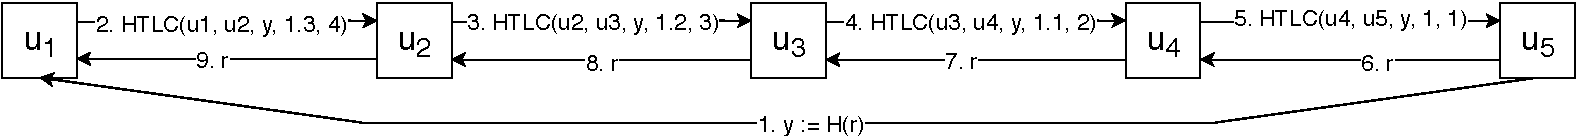
\includegraphics[width=\textwidth]{htlc-figure}
	\caption{An HTLC-based payment in the LN. The node $u_1$ pays $u_5$ using $u_2$, $u_3$ and $u_4$ as intermediaries. 
		Here we assume that each node charges a fee of $0.1$ and time is measured in days.\label{fig:htlc}}
\end{figure*}

\paragraph{Single-channel transactions}

To send a payment to Bob, Alice negotiates a new channel state.
Each channel state is reflected in a \textit{commitment transaction}.
A commitment transaction spends the output of the funding transaction and re-distributes the coins between Alice and Bob.

More precisely, each channel state is encoded in a \textit{pair} of commitment transactions: one for Alice and one for Bob.
These transactions are symmetric: they enforce a timelock on the party that holds the transaction.
In particular, Alice's version of commitment transactions allow her to redeem her output only after a timeout, and Bob's version imposes analogous restrictions on his output.
This enables the revocation mechanism (described below), which provides economic security guarantees to LN channels, assuming the parties are watching the blockchain sufficiently often.

Outputs of commitment transactions are called \textit{Hash time-locked contracts}, or \textit{HTLC}s.
HTLC is defined by a Bitcoin script that gives the funds either to one party, if it provides a pre-image of a given hash, or to the other party after a timeout.

An HTLC is an excerpt from the Bitcoin's scripting language that 
permit a node ($u_1$) to lock $x$~coins in a channel between two nodes ($u_1$ and $u_2$) 
and release them according to the encoded conditions.
The terms for the HTLC($u_1, u_2, y, x, t$) are defined with a hash value $y := H(r)$, 
where $r$ is chosen uniformly at random, 
an amount $x$ of coins, and a timeout $t$, as follows: 
(i) If $u_2$ reveals a value $r$ such that $H(r) = y$ before $t$ expires, $u_1$ pays $x$ to $u_2$; 
(ii) if $t$ expires, $u_1$ receives $x$ back.

For instance, if Alice wants to send $x$ coins to Bob, she first asks him for a \textit{payment hash}.
Bob generates a random number $r$ and send its hash $H(r)$ to Alice in a message called an \textit{invoice}.
Alice then \textit{offers} Bob an HTLC that would give him $x$~coins if he provides the preimage of $H(r)$ before time $t$, or return the coins to Alice otherwise.
Therefore an HTLC can be \textit{resolved} in one of two ways: either Bob provides the preimage and \textit{redeems} the coins before time $t$, or Alice gets the coins back.
A payment channel can keep track of multiple unresolved HTLCs concurrently, which are also called \textit{in-flight} HTLCs.


\paragraph{Multi-channel transactions}

A multi-channel transaction leverages a path of channels between a sender and a receiver (who might not share a channel between them).
%A chain of single-channel updates are set up using HTLCs with the \textit{same} hash value.
%This ensures atomicity: either all channels are re-balanced or none of them are.

LN relies on HTLCs to enable multi-hop transactions. 
The final recipient generates a random $r$ and sends its hash $H(r)$ to the initial sender.
All HTLCs along the path use the same hash value $y=H(r)$ aiming to achieve atomicity expecting that none of the intermediate balances can be updated before the receiver reveals $r$, and all of them can be updated after that.
The receiver redeems the payment from the last channel by revealing $r$, which in turn allows all intermediary channels to be re-balanced accordingly.

An illustrative example of an HTLC-based transaction is depicted in~\cref{fig:htlc}.
Here, the user $u_1$ transfers $1$~coin to $u_5$ using $u_2$, $u_3$ and $u_4$ as intermediaries.
For that, $u_5$ locally chooses a value $r$ uniformly at random, computes the cryptographic challenge for the HTLC as $y := H(r)$, and sends $y$ to the sender in an \textit{invoice} (step 1).
Then, the payment starts with a commit phase (steps 2-5) where every pair of nodes, starting from the sender, establishes an HTLC using $y$.
After the commit phase is finished, the transaction enters the release phase.
Here, the receiver reveals $r$ to $u_4$ to fulfill the contract (step 6), triggering the release phase where every pair of nodes fulfills their contract from the receiver to the sender (steps 6-9).

Intermediary users may charge a fee for the forwarding service provided. 
For instance, $u_2$ receives $1.3$~coins but only forwards $1.2$~coins, getting a fee of $0.1$~coins.
No fees are collected if a payment fails, as all pending balance updates roll back.
In the actual LN protocol, the fee consists of two parts: a constant \textit{base fee} for each payment and a \textit{fee rate} proportional to the value being transferred.
\footnote{Note that LN fee structure is different from fees on L1, where the fee is proportional to transaction weight (roughly speaking, size in bytes) but does not account for the amount of value being transferred. This may result in the economics of LN fees being significantly different from that in Bitcoin. As of 2020, LN fees are largely non-economical~\cite{Beres2019}.}

Note that the time parameter of the contracts along the path is decreasing to ensure a safety margin between HTLC timeouts.
For instance, the HTLC between $u_1$ and $u_2$ sets a timeout of four days, whereas the timeout in the HTLC between $u_2$ and $u_3$ is only three days.
This ensures that $u_2$ has enough time to settle the contract with $u_1$ after receiving $r$ from $u_3$, even if $u_3$ reveals the preimage just before the corresponding timeout expires.
There is an inherent trade-off regarding timeout lengths.
Channels with short timeouts open the risk of not being able to dispute a fraudulent transaction in case of blockchain congestion, and long timelocks open up a DoS vector, where an attacker can route many unsettled payments through a channel and effectively block it until the timelock expires.

Multi-path payments use onion routing to enforce the order of intermediary nodes.
Each intermediary node only knows the immediate previous and next nodes, but not the final sender or receiver and not its position in the path.


\subsubsection*{Channel closure}

A channel is closed when a transaction that spends the funding transaction's output gets confirmed on-chain.
This may happen in one of three ways:

\begin{itemize}
	\item Collaborative closure. Alice signals the intent to close the channel, and Bob cooperates in signing the transaction that reflects the latest channel state. This results in one on-chain transaction to close a channel, and no delays for both parties. Both parties must be online and cooperating.
	\item Non-cooperative closure without breach. Alice signals the intent to close the channel, but Bob does not respond. In this case, Alice commits the latest commitment transaction on the blockchain. Bob can redeem his output immediately, but Alice has to wait until a timeout expires. This is a safety measure to provide Bob with an opportunity to broadcast a \textit{justice transaction} (see below).
	\item Non-cooperative closure with breach. Alice broadcasts an old commitment transaction in an attempt to close the channel with an outdated distribution of funds (thus potentially stealing from Bob). If Bob does not react before the timelock on Alice's output expires, Alice can redeem her output, and the channel is closed.\footnote{From the on-chain point of view, a non disputed non-cooperative close is indistinguishable from a non-cooperative close without a breach: the blockchain does not know whether a commitment transaction is the last one, unless this fact is disputed.} If Bob is online and notices the breach before the timeout, he broadcasts the latest commitment transaction, which allows Bob to spend Alice's output before she can, punishing her for the cheating attempt.
\end{itemize}

This revocation mechanism is the key element of LN, which allows LN channels to have an unlimited lifetime (the parties do not have to close the channel if none of them wants to) and to support payments in both directions.
This makes the LN superior to earlier payment channel designs.
However, the trade-off here is that parties must be online to notice potential malicious channel closures and broadcast justice transactions.
This functionality can be outsourced.
Entities that watch the blockchains for malicious channel closures and dispute them on behalf of a user are called \textit{watchtowers}.
Implementing effective, economically incentivized, and privacy-preserving watchtowers in an active area of research~\cite{McCorry2019}.

LN's revocation mechanism has proved effective as a deterrence against malicious channel closures.
As of July~2019, there has been only 241 channel closures followed by a justice transaction -- 0.7\% of the number of Lightning channels at that time~\cite{BitMEXLN3}.
\footnote{The research is based on the LN's on-chain footprint and is not absolutely accurate. A non-cooperative closure followed by a justice transaction may also happen without malicious intent, for example, as a result of a broken backup restore (where Alice's node "forgets" about the latest state and broadcasts an earlier state assuming it is the latest one).}


\subsection{P2P network and routing}

In the description of multi-channel transactions, we noted that the sender arranges a series of HTLCs along the path towards the receiver.
But how does the sender construct such a path?

LN nodes gossip about newly opened channels that are marked as available for routing.
Based on this information, each node maintains a local view of the network, and uses it to calculate routes to the receiver.
As total channel capacities are known, the sender only considers channels with the capacity larger than $X$ for a payment of amount $X$.
However, this is insufficient to prevent routing failures, because the distribution of funds in channels is not known.
The ability of channel parties to send or forward payments is limited by their \textit{local} channel balances.
Initially, if Alice opens a channel with Bob, all funds are on her side.
This means that she can send up to the total capacity, but she can not receive.
As the local balances change, the routing capabilities of the channels in both directions are also changing.
This makes routing not very reliable, especially for larger payment amounts.

In case of payment failure, an error message notifies the sender which channel has failed.
The sender would presumably try to send the payment again along a new route without the failed channel.
This procedure repeats multiple times until a payment succeeds.
Optimizing path finding for payment channel networks is an active area of research~\cite{Pickhardt2019a, Prihodko2016, Grunspan2018, Pickhardt2019, Piatkivskyi2018, Sivaraman2018, Bagaria2019, Roos2018}.


\section{Privacy in payment channel networks}

There are substantial differences in the privacy models of first- and second-layer blockchain protocols.
In contrast to Bitcoin transactions, which are openly broadcast, LN payments are only sent to a short chain of randomly chosen nodes.
Due to onion routing, each intermediary node only knows the previous and the next hops, but not the whole route and even not its position in the route.
This leads to an assumption that Lightning provides more privacy than Bitcoin.

\todo[inline]{Outline differences}




\chapter{Probing Lightning channel balances}

\label{Chapter06LNprobing}

The LN protocol provides no way for a node to know how funds are split in remote channels.
But how private is this information in practice?
In this Chapter, we show that a low-resource attacker can infer balances of most of the channels.\footnote{This Chapter is based on~\cite{Tikhomirov2020}.}
We describe an algorithm that reveals channel balances using \textit{probing} -- sending a fake payment (referred to as a \textit{probe}) and observing the resulting error.
We substantially improve upon similar approaches described in the literature in terms of accuracy and cost.
Our technique scales to the whole network and achieves high precision.
It requires moderate capital commitment, half of the channels can be probed in $21$~seconds.
The attacker's capital is not spent, but only temporarily locked up.
Compared to previous approaches~\cite{HerreraJoancomarti2019, Dam2019}, we can probe \textit{remote} channels (i.e.,~without establishing a channel with one of their endpoints).
This greatly reduces the requirements of the attack both in terms of time and capital.
We test our proof-of-concept implementation on Bitcoin testnet and successfully probe a significant portion of its channels.
We also outline potential countermeasures, which include modification in error handling, sharing channel balances explicitly, and \textit{just-in-time} (JIT) routing.

On a more general note, we raise a question of the \textit{privacy-efficiency trade-off} in the LN\@.
At the moment, LN nodes cannot use balance information for routing, which leads to failed payments, but balances are extractable by an attacker anyway.
Can we strike a better balance between balance privacy and routing efficiency?
Answering this question remains an exciting avenue for future work.


\section{Probing algorithm}
\label{sec:probing}

\subsection{Overview}

As described in Chapter~\ref{Chapter05IntroLightning}, a payment channel operates as follows.
Two parties lock funds in a multi-signature transaction output and then modify the distribution of funds in a sequence of nearly instant off-chain transactions.
LN nodes gossip about channels available for routing and their total capacities.
To issue a multi-hop payment, the sender creates a route based on its local knowledge of the network.
The current channel balances are not announced.

Consider two LN nodes that share a channel.
Let us denote the total capacity of the channel as $c$.
LN channels are bidirectional.
Without loss of generality, let us denote one of the nodes as \textit{source} (with balance $b_s$) and the other as \textit{destination} (with balance $b_d$).\footnote{As per BOLT specification, the source is defined as the node with an alphanumerically smaller node ID.}
By definition, $c = b_s + b_d$.
Our goal is to determine how $c$~is split between $b_s$~and~$b_d$.
For concreteness, for each channel, we estimate $b_s$, and refer to it simply as $b$.

In a nutshell, our algorithm consists of the following steps:
\begin{itemize}
	\item set up a Lightning node;
	\item open a few \textit{entry channels} to manually selected nodes (referred to as \textit{entry nodes});
	\item compile the list of channels for probing;
	\item for each channel in the list, do a binary search for the value of~$b$~by sending fake payments through routes ending with the chosen channel.
\end{itemize}

\subsection{Assumptions}

To be suitable for probing, the channel must be \textit{active} (available for routing) and \textit{live} (responding to requests).
We assume that nodes follow the BOLT specification (in particular, they return errors as prescribed).

\paragraph{Error interpretation}
Our method uses two types of errors, which have a broader semantics than our method is aware of.
\texttt{temporary\_channel\_failure} (\texttt{UPDATE|7}) is returned if a forwarding node "was unable to handle this HTLC, but may be able to handle it, or others, later".
We interpret this error as "insufficient balance", though there may be other reasons for a channel to be temporarily unavailable.
\texttt{incorrect\_or\_unknown\_payment\_details} (\texttt{PERM|15}) is returned if "[t]he payment\_hash is unknown to the final node, the payment\_secret doesn't match the payment\_hash, the amount for that payment\_hash is incorrect or the CLTV expiry of the HTLC is too close to the current block height for safe handling".
We interpret this error as only the first of the listed conditions.
The payment hash is definitely unknown to the receiving node, as we generated it randomly.
Other conditions should generally not hold: the amount and the HTLC expiry date should be consistent, as we rely on standard functionality of c-lightning to construct payments.
We assume it to be compliant with the specification and well-tested.
Experiments on our own channels showed that these types of errors are indeed returned under the conditions relevant for our experiment.

\paragraph{A note on probing directions}
Our probing algorithm is agnostic to the direction of probing payments.
For instance, sending a probe via a route ending in "Alice -- Bob" theoretically gives the same information as via a route ending in "Bob -- Alice".

However, channel directions may have different properties in practice.
Each channel party controls its channel direction.
Alice sets the routing policy in the direction to Bob, and Bob sets the policy in the direction to Alice.
Some channels are is only partially active: i.e.,~Alice allows routing to Bob, but Bob does not allow routing to Alice.
To extract the maximum amount of information, we probe channels in both directions.

Probing from both sides also helps us overcome the technical issue with large channels (discussed below).
Due to the limitation on LN transaction amount, we cannot probe very large channels.
However, if the capacity of a large channel is skewed, we can get the required information by probing it from the "smaller" end.
For clarity, we omit this implementation detail from the algorithm description.

\paragraph{A note on applicability}
Our experiments are meant to show the feasibility of the probing technique, but the results from testnet can not be directly applied to mainnet.
In particular, the mainnet LN contains four times more channels than the testnet LN\@.
Therefore, probing the whole LN on mainnet would take ore than two~days instead of~$14$~hours.
We note that the attacker can still target specific channels, for instance, those belonging to a particular service provider.
Probing tens or hundreds of chosen channels is feasible in terms of time.
It would give the attacker valuable insights into the victim's financial situation.


\subsection{Selecting channels for probing}

First, we establish the list of channels that are active and live.
We define a channel as \textit{active} if at least one of its two directions is announced as active in the gossip data.
To determine liveness, we use the heuristics presented in Algorithm~\ref{alg:select-channels}.

\begin{algorithm}
	\KwData{Gossip data}
	\KwResult{Channels selected for probing}
	\For{node in gossip data} {
		connect to node\;
		\If{connection established}{add node to live nodes\;}
	}
	\For{channel in gossip data}{
		\If{source and destination in live nodes}{
			add channel to channels to probe\;
		}
	}
	\For{channel in gossip data} {
		send a 1000~sat probe\;
		\If{error returned}{add channel to channels to probe\;}
	}
	\caption{Selecting channels for probing.}
	\label{alg:select-channels}
\end{algorithm}

\paragraph{Heuristic 1: Connecting to nodes}
For a channel to be live, both its parties must be live.
We extract a list of nodes from gossip data and establish a P2P connection to each of them.\footnote{Establishing a P2P connection is nearly instant and, unlike opening a channel, does not require capital commitment.}
We consider a channel live, if both its parties are live.
We close all the connections after this step, except for the connections to our entry nodes.

\paragraph{Heuristic 2: Pre-probing}
To further optimize probing, we introduce an additional pre-probing step.
We send a probe of~$1\,000$~satoshis to every channel marked as active in the gossip data\footnote{We use the same probing function as for the main probing described below.}.
If we get no response, we consider the channel dead and do not consider it in the main probing step.
For the first round of probing, we consider all live channels, where a channel is defined as live if either heuristic 1 or heuristic 2 classify it as live.

\paragraph{Heuristic 3: Liveness detected during probing}
Each probe results in an error propagated back to the sender.
During the first probing round, we expand our list of live channels.
If we issue a probe along the route of channels $c_1, c_2, \dots, c_n$~and receive an error from channel $c_i$, we conclude that all preceding channels $c_j, j<=i$~are live.
If any of~$c_j$~is not on our live channels list, we add it.
During the second probing round, we use the updated live channels list.


\subsubsection*{Channel order}
We say that channel $c_1$~is \textit{closer} to us than channel $c_2$, if the shortest route from our node to one of the endpoints of~$c_1$~is shorter than that for $c_2$.
We informally refer to a channel as \textit{important}, if a large share of our probes is forwarded through it.
Our method is agnostic to the order in which we probe the channels.
However, we choose to probe the "closer" and "more important" channels first.
The rationale is that it is beneficial to first probe the channels that are often used as intermediary hops.
Knowing their balances allows us to avoid sending payments that would certainly fail due to insufficient balance at an intermediary hop.

We probe channels in the following order:

\begin{itemize}
	\item the "first layer" -- channels adjacent to the entry nodes;
	\item channels between hubs -- channels connecting nodes out of~$1\%$~of the most connected nodes (if not already probed);
	\item the "second layer" -- channels adjacent to the "first layer" (if not already probed);
	\item all other channels (if not already probed).
\end{itemize}


\subsection{Probing}

After compiling a list of live and active channels, we issue a series of probes to each of them.

Recall that in the normal course of operation the receiver of the payment generates a random value $r$~and sends its hash to the sender.
The sender then creates a series of HTLCs with the common hash value $h = H(r)$.
The key idea behind probing is sending unsolicited payments using random values instead of~$H(r)$.
Such payments fail in any case.
However, we can obtain the information on channel balances based on which error occurred and where.
In particular, we can infer whether the balance of the erring channel is higher than the probing amount $a$.
Intermediary nodes can not distinguish randomly generated and genuine payment hashes.
They will therefore forward our probes as usual payments.
If all channels along a route have sufficient balances (higher than $a$), the probe only fail at the last step.
The final recipient finds out that it does not know the preimage for the payment hash and emits the corresponding error message.
If any channel has insufficient capacity, the payment fails at that channel, before reaching the final recipient.

Let $c_1, c_2, \dots, c_n$~be a sequence of channels in a route, and~$b_i$~be their respective balances.
Let $c_j$~be the erring channel.
After each probe with an amount $a$, we obtain the following information:
\begin{itemize}
	\item $b_i > a$~for $i<j$;
	\item $b_j < a$~if the error is "insufficient capacity", or $b_j > a$~if the error is "unknown preimage".\footnote{The latter is only possible if $j=n$.}
\end{itemize}

The probing algorithm for a single route is presented in Algorithm~\ref{alg:probe-route}.

\begin{algorithm}
	\KwData{Route and amount to probe}
	\KwResult{Updated balance estimates for channels in route}
	send payment along route\;
	\For{channels before erring channel} {
		$b_{min} = a$\;
	}
	\For{erring channel}{
		\If{insufficient funds}{
			$b_{max} = a$\;
		}
		\If{unknown preimage}{
			$b_{min} = a$\;
		}
	}
	\caption{Probing a route.}
	\label{alg:probe-route}
\end{algorithm}


For each channel, we keep a lower ($b_{min}$) and an upper ($b_{max}$) bound for its balance $b$.
Initially, $b_{min}=0$~and~$b_{max}=c$.
At each probing step, we aim at shrinking this interval with binary search, i.e.,~by issuing a probe with the amount of~$\frac{1}{2} (b_{min} + b_{max})$.
If the midpoint between $b_{min}$~and~$b_{max}$~is larger than the maximum HTLC amount allowed by the specification, we decrease it to that maximum minus a safety margin.
The algorithm for all channels selected for probing is presented in Algorithm~\ref{alg:probe-channels}.

\begin{algorithm}
	\KwData{Gossip data}
	\KwResult{Improved estimates for channels}
	SelectChannelsForProbing\;
	\For{channel in channels for probing} {	
		$b_{min} = 0$\;
		$b_{max} = c$\;
		\For{number of probings per channel} {
			\For{number of attempts per probing}{
				GetRouteToTargetChannel\;
				ProbeRoute\;
				\For{channel in route}{
					\If{channel is live and not marked as live}{
						mark channel as live
					}
				}
				\If{target channel estimates updated}{
					continue\;
				}
			}
			\If{required precision reached}{
				continue\;
			}
		}
	}
	\caption{Probing all channels.}
	\label{alg:probe-channels}
\end{algorithm}


\paragraph{Choosing routes}

For each probe for a chosen \textit{target channel}, we select routes with the following objectives:
\begin{itemize}
	\item the target channel is the last channel in the route;
	\item all previous channels in the route have sufficient balances (to the best of our current knowledge) to forward the probe amount.
\end{itemize}

The route generation algorithm is presented in Algorithm~\ref{alg:find-route}.

\begin{algorithm}
	\KwData{target channel, amount $a$}
	\KwResult{Route to target suitable for $a$}
	\For{channels adjacent to destination} {
		\If{channel is not target}{
			add channel to excluded channels\;
		}
	}
	\For{all channels}{
		\If{$a > c_{max}$}{
			add channel to excluded channels\;
		}
	}
	\While{route is bad}{
		get route to target without excluded channels\;
		\For{channel in route}{
			\If{$a > b_{max}$}{
				route is bad\;
			}
		}
		route is good\;
	}
	\Return route\;
	\caption{Getting a route to the target channel.}
	\label{alg:find-route}
\end{algorithm}

We rely on the built-in functionality of our LN node (c-lightning) to generate routes\footnote{Internally, it uses Dijkstra algorithm.}.
The c-lightning API allows us to customize routes, offering an option to exclude specified nodes and channels.
We use this functionality to pre-filter suggested routes based on the information we have obtained through probing so far.
If we know that a balance of some channel in a suggested route is insufficient, we exclude such channel from consideration for the current probe.
This allows us to avoid sending probes through routes with insufficient balances in intermediary channels, hence speeding up our algorithm.

Finally, we perform the second probing pass to probe the channels that have been only detected as live during the first pass (the third liveness heuristic described earlier).

\paragraph{Channel information coefficient}
To measure the effectiveness of our technique, we introduce the \textit{channel information coefficient}.
Let $c$~is the original channel capacity, and~$b_{max}$~and~$b_{min}$~be our upper and lower bound estimates for $b$.
Then the information coefficient is defined as:

\[i = 1 - \frac{b_{max} - b_{min}}{c}\]

Thus, $i = 0$~means that we do not know any extra information about $b$~in addition to public knowledge.
The value $i = 1$~means that we know $b$~precisely.


\section{Experimental setup}

We implemented the algorithm described in~\cref{sec:probing} as a c-lightning plugin.
%C-lightning~\cite{clightning} is one of the three major LN implementations, alongside LND~\cite{LND} and Eclair~\cite{Eclair}.
The plugin functionality allows developers to integrate Python code with the c-lightning node~\cite{clightningPlugins}.
%For ethical reasons and to be in compliance with privacy-related regulations, 
We only collected data from Bitcoin~testnet.
We tried to perform at least $7$~probings per channel.
This means that in a successful probing we shrank the $[b_{min}, b_{max}]$~interval to $\frac{1}{128}$~of its initial length, determining $b$~with the precision better than $1\%$.

\paragraph{Entry nodes}
We launched our own LN node\footnote{c-lightning version \texttt{v0.8.0-40-g899f5de}.} and funded it with testnet coins.
Then, we established five~entry channels opened to handpicked nodes with high connectivity and liquidity.
Four of our channels had the maximum standard capacity of~$0.167$~BTC\@.\footnote{LN limits the channel capacity at $0.167$~BTC\@. Larger channels can be created with a special command line argument and are sometimes referred to as \textit{wumbo channels}.}
One entry channel had the capacity of~$0.043$~BTC\@.
We choose nodes to connect to based on the following requirements (as reported by 1ML~\cite{1MLTopConnected}):
\begin{itemize}
	\item well-connected and well-capitalized;
	\item located relatively close to our node (i.e.,~in Europe) to decrease latency.
\end{itemize}

\paragraph{Choosing the timeout}
One of the decisions we had to make is to set a timeout after which we declare a channel unresponsive and move to the next one.
The LN protocol does not prescribe how quickly a node should react.
The only time limitation is the HTLC timeout, which is usually on the order of hours or days.
Therefore, to probe all channels in reasonable time, we chose a timeout of~$10$~seconds.
Our later results showed that this was a reasonable trade-off between probing speed and accuracy.

\paragraph{Route selection}
As described earlier, we generated routes with the standard c-lightning \texttt{getroute} routine, and filtered out routes that included channels with insufficient balance.
Note that route generation is a local operation.
In our experiments, one route generation took under $10$~ms.
This is two orders of magnitude lower than the average probe response time ($3$~seconds).

In our main experiment, we performed $12\,895$~payments.
We rejected $96\,768$~routes because of low balance.
That is, we filtered out around $8$~routes per payment.
Hence, our method of route generation did not significantly increase the time of our experiment.
This approach may be improved with custom route generation.

Another trade-off we had to address is the maximum route length.
The LN protocol limits the length of a route to $20$~channels.
Longer routes allow collecting more information per probe, but increase the probability of failure at one of the intermediary channels.
For our experiment, we limited the length of routes to $10$~channels.

\paragraph{Hanging HTLCs}
Our method assumes that for each probe an error is returned quickly (within seconds, as Figure~\ref{fig:route-length-timings} shows).
If some intermediary hop does not return an error, we are left with an unresolved in-flight HTLC that we call \textit{hanging}.
Hanging HTLCs occupy the capacity of our channels, preventing us from issuing large probes from the affected channel.
The protocol does not allow to cancel them unilaterally, and closing a channel involves long timeouts until the funds are available and can be put into a new channel.
Therefore, we use multiple entry channels, so that we can tolerate some hanging HTLCs in some of them.
This issue is similar to our own attack presented in Chapter~\ref{Chapter08HTLClimit} and the one described in~\cite{Mizrahi2020}.


\section{Results} \label{sec:results}

We performed the experiment on 26~February~2020.
At that time, the LN on Bitcoin~testnet contained $1\,974$~nodes and~$5\,884$~channels (including $2\,527$~announced as active).
The initial estimate showed that $207$~nodes and~$1\,625$~channels were live.
We detected $3$~additional live channels during the first probing pass.
The strongly connected component of the live subgraph contained $1\,489$~channels.
The other $139$~channels where pointing towards nodes for which we could not get meaningful error messages.

In total, we sent $12\,895$~probes: $3\,153$~($24.45\%$) during the pre-probing and~$9\,742$~($75.55\%$) during the main probing phase.
Out of~$9\,742$~probes in the main phase, $8\,256$~($84.75\%$) returned errors which we could use to improve the estimates of balances on payment channels ("channel temporary unavailable" and "incorrect or unknown payment details").
Our code was running for~$14$~hours and~$6$~minutes. % 50770 seconds
Probing $1\,628$~live channels took $65\%$~of the time (roughly $9$~hours).
The rest was spent on slow-responding channels or channels which replied with an unexpected error.


\subsection{Probing times}

First, we consider probing times of individual probes.
Figure~\ref{fig:route-length-timings} shows the distribution of probing times for various route lengths.

\begin{figure}[ht]
	\centering
	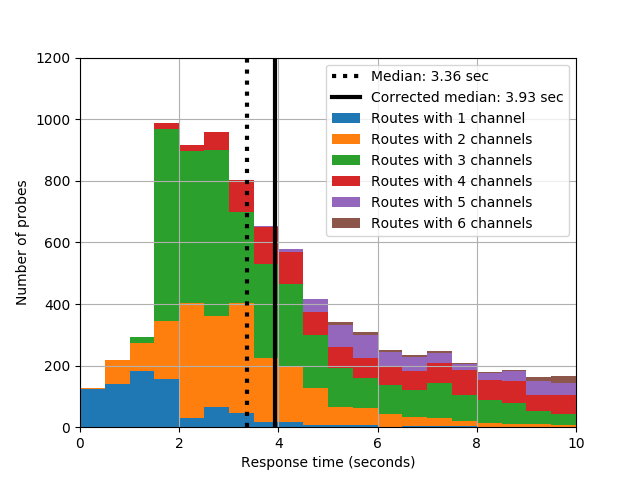
\includegraphics[width=0.8\textwidth]{route-length-timings.png}
	\caption{The distribution of probes (onions) by response time.}
	\label{fig:route-length-timings}
\end{figure}

Nearly all probes $3$~hops and shorter return within $10$~seconds.
The median of the $8\,256$~probes is at $3.36$~seconds.
Recall that $15.25\%$~of the probes timed out or returned an error that we could not interpret within out algorithm.
The corrected median without the timed out and erring probes is $3.93$~seconds. 
We conclude that the cutoff at $10$~seconds presents an acceptable trade-off.
Note also that the diameter of the strongly connected component on the LN is just $3$.\footnote{It is not always possible to use the shortest route, as it may not have sufficient balances in all channels.}

Next, we consider the time it takes to probe a single channel.
With the parameters we have chosen, each probe can not take longer than $70$~seconds ($7$~probes of up to $10$~seconds each).
For each channel, we add up the times of probes sent to this channel.
Figure~\ref{fig:channel-timings-CDF} shows the cumulative distribution function of channels by the total time spent probing them.
We observe that $50\%$~of channels can be probed in less than $21.2$~seconds.

\begin{figure}[ht]
	\centering
	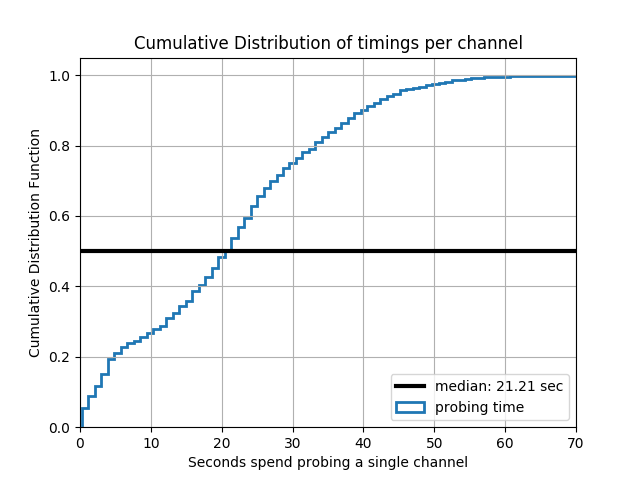
\includegraphics[width=0.8\textwidth]{channel-timings-CDF.png}
	\caption{Distribution of channels by total probing time.}
	\label{fig:channel-timings-CDF}
\end{figure}


\subsection{Probing coefficients}

We used the channel information coefficient to measure how much information we obtained for each channel.
At the time of the experiment, the LN specifications limited the value of a single payment to $0.043$~BTC\@.
We denote channels with the capacity more than two times that (i.e.,~$2 \times 0.043 = 0.086$~BTC) as \textit{large channels}.
Other channels are referred to as \textit{small}.
All small channels can in principle be fully probed.
A large channel can only be fully probed, if the local balance at one of its endpoints is lower than the maximum payment amount.

\begin{figure}[ht]
	\centering
	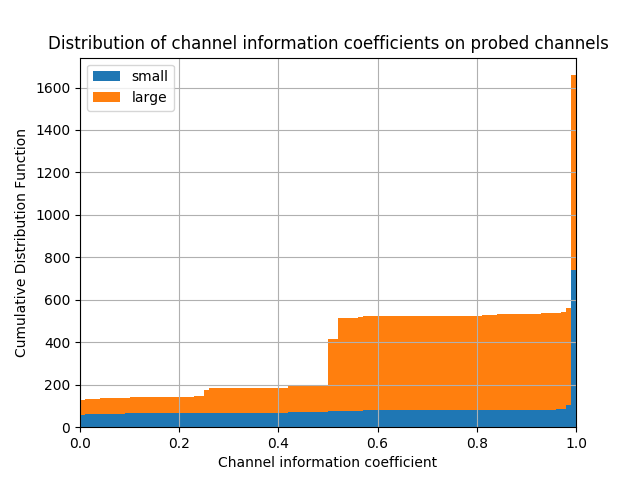
\includegraphics[width=0.8\textwidth]{cdf-channel-coefficients.png}
	\caption{Distribution of channels by the obtained information coefficient.}
	\label{fig:cdf-channel-coefficients}
\end{figure}

Figure~\ref{fig:cdf-channel-coefficients} represents the distribution of channels by their information coefficients.
We obtained full balance information on over $1\,000$ of~$1\,628$~channels.
Note that the jump at $0.5$~for the large channels is expected:the maximum standard channel capacity ($0.167$~BTC) is approximately four times higher than the maximum HTLC amount ($0.043$).
Consider a channel with the total capacity of~$0.167$~BTC and the local balance between $0.043$~BTC and~$0.167 - 0.043 = 0.124$~BTC\@.
We probe this channel from both sides and receive the "unknown hash" error in both cases.
From that we conclude that the local balance is indeed between $0.043$~BTC and~$0.124$~BTC\@.
This estimate yields a channel information coefficient of~$0.515$.
However, with our current technique we cannot improve it.

\subsection{Distribution of channels in routes}

We also wanted to understand how often we send probes through each channel.
As Figure~\ref{fig:channel-frequency-distribution} shows, most of our routes go through the same few channels.
It is partially explained by the fact that all routes pass through one of our own entry channels.
%We suggest that this distribution, which seems to follow the power law, is consistent with the properties of a small world network with a small diameter.

\begin{figure}[h]
	\centering
	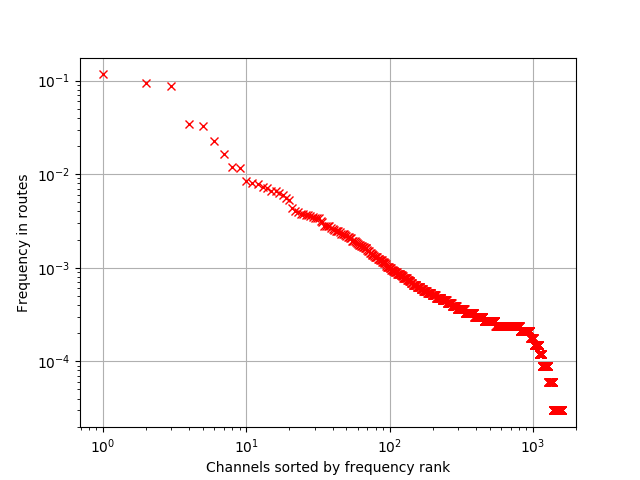
\includegraphics[width=0.8\textwidth]{channel-frequency-distribution.png}
	\caption{Distribution of relative frequencies of channels in routes.}
	\label{fig:channel-frequency-distribution}
\end{figure}


\subsection{How balanced are the channels?}

A Lightning channel is informally called \textit{balanced} if the parties have roughly equal balances.
We introduce the \textit{balance coefficient} to quantify this.
The balance coefficient represents the distance from the actual channel balance to $0.5$~of the total capacity, where $b$~is the estimated local balance and~$c$~is the total channel capacity:

\[c_{bal} = 0.5 - \frac{|b-c|}{c} \]

$c_{bal} = 0$~means the channel is unbalanced: the whole capacity is on one side.
$c_{bal} = 1$~means the channel is perfectly balanced: the two sides have equal balances.

\begin{figure}[h]
	\centering
	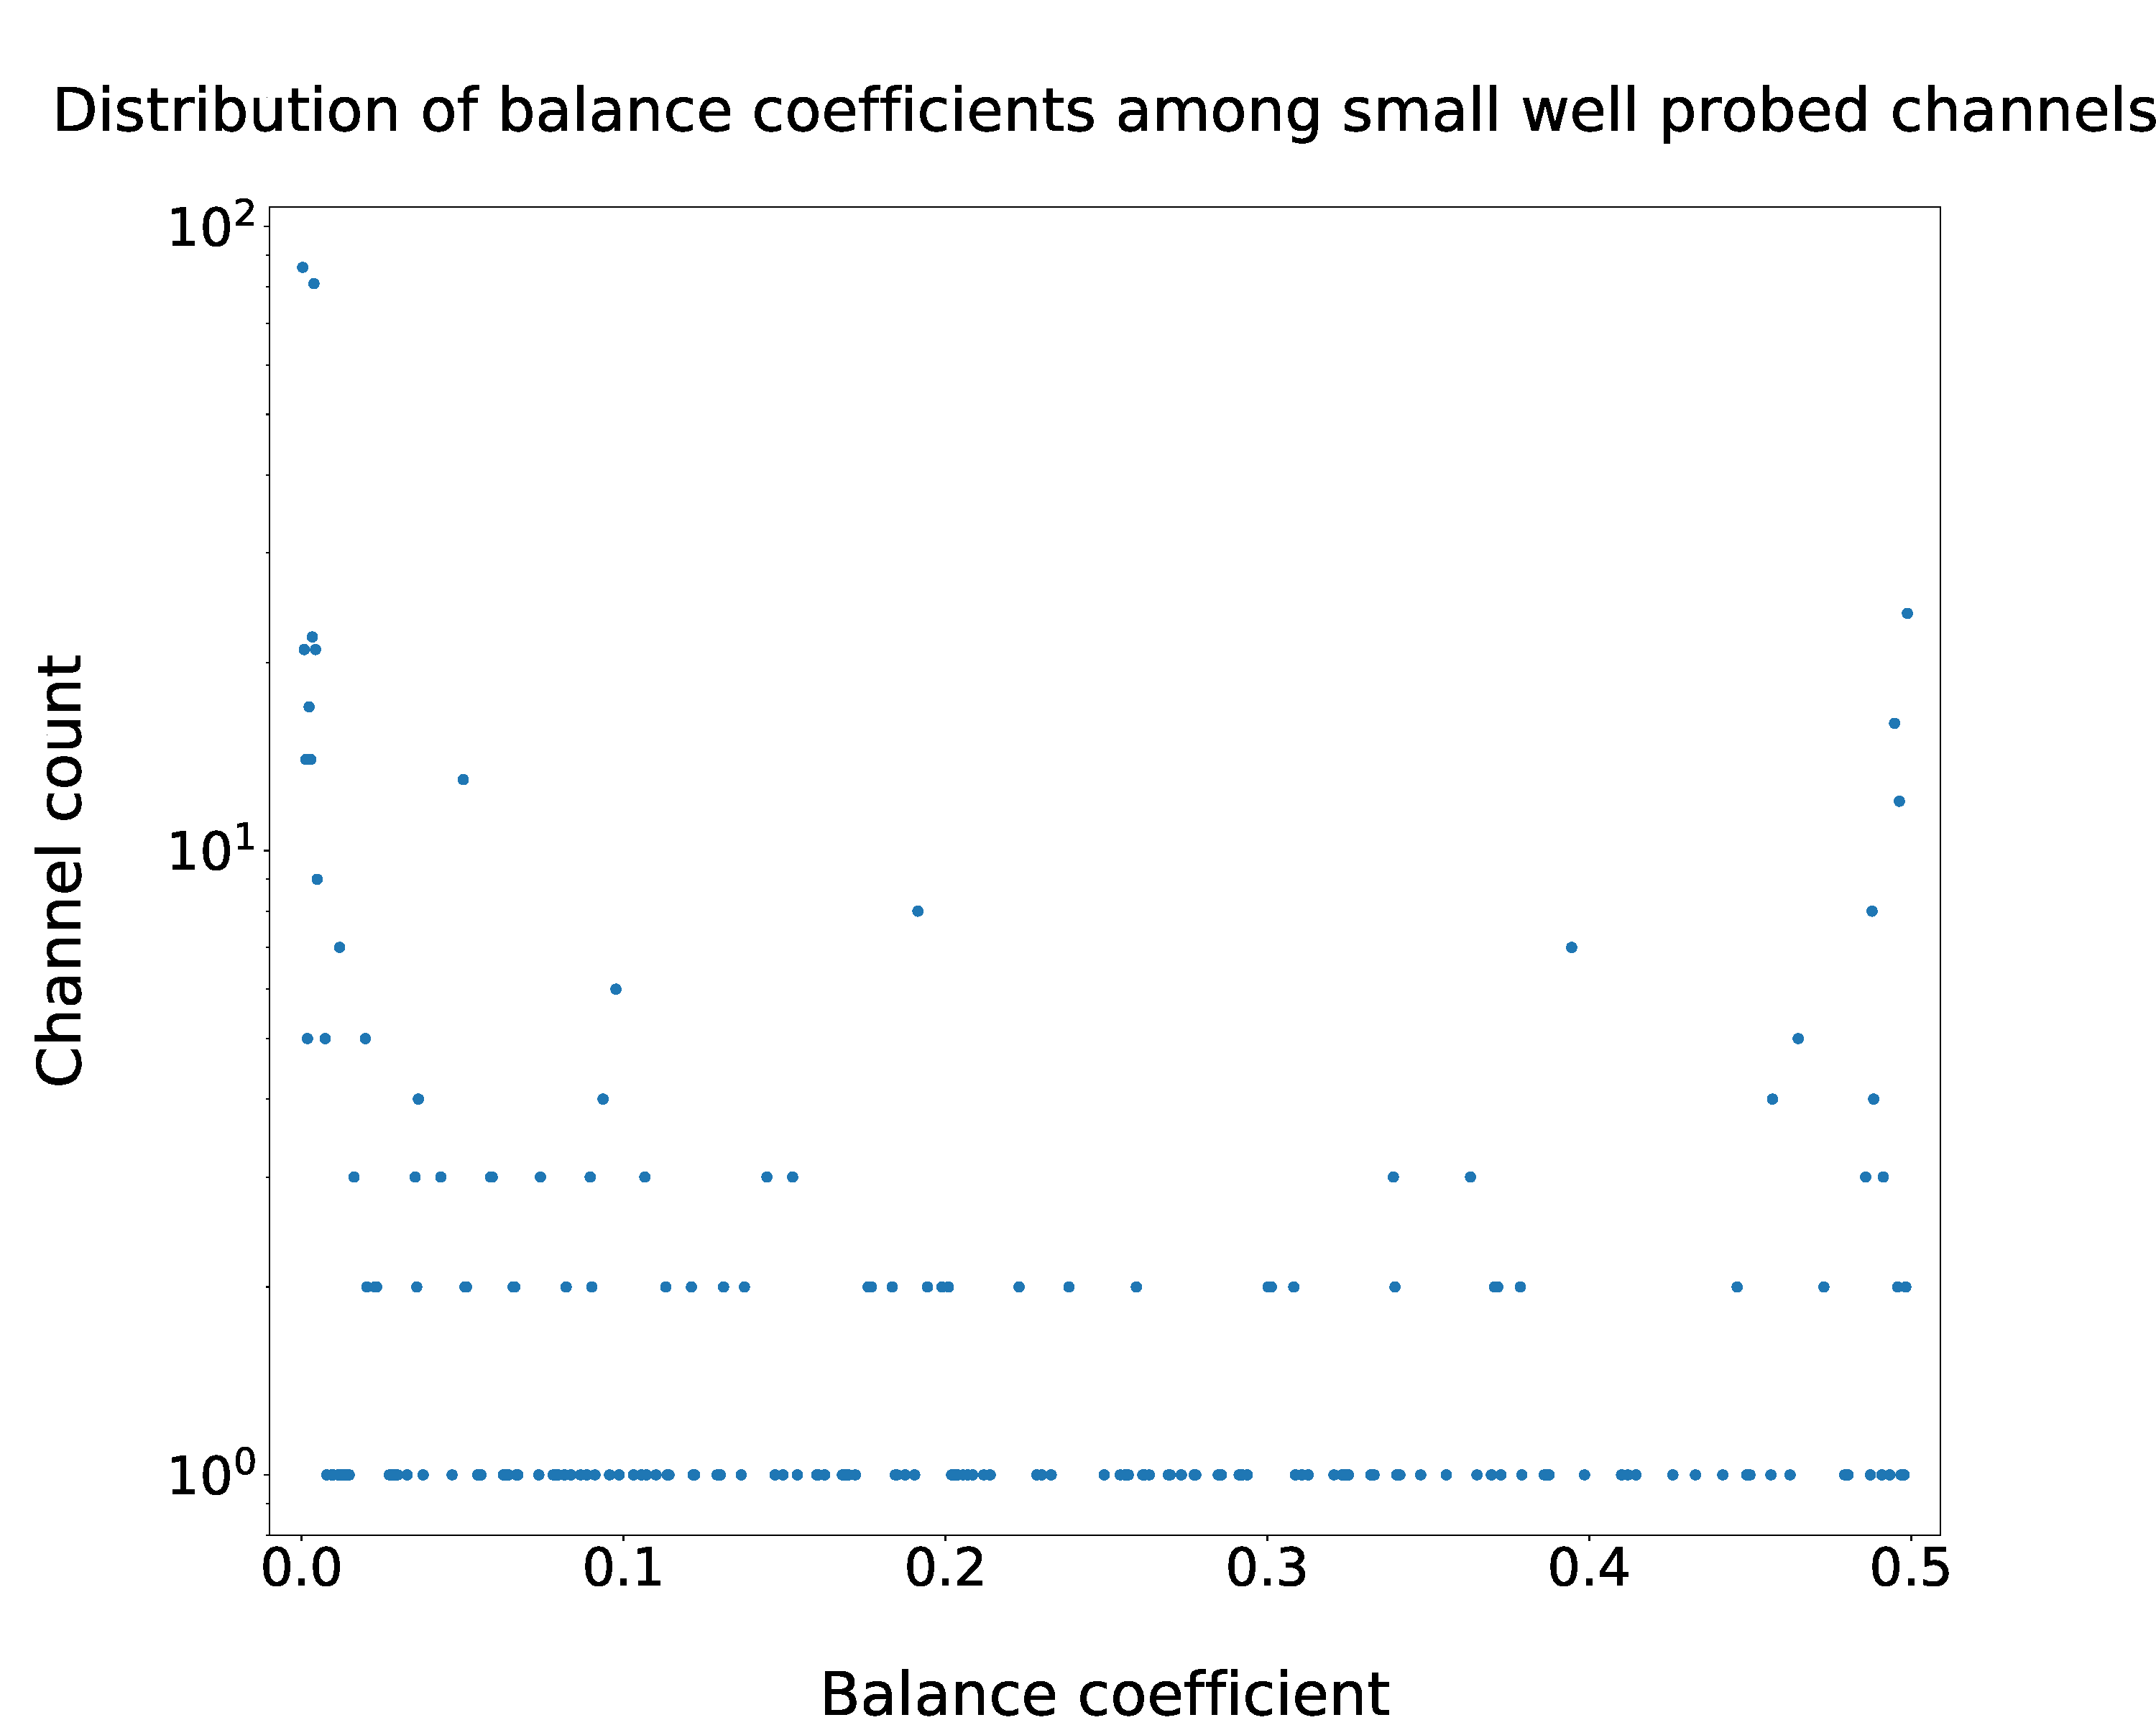
\includegraphics[width=0.8\textwidth]{balance-coeff-histogram.pdf}
	\caption{Distribution of balance coefficients.}
	\label{fig:balance-coeff-histogram}
\end{figure}

Figure~\ref{fig:balance-coeff-histogram} depicts the distribution of balance coefficients among "small" channels that we were able to probe with high accuracy (information coefficient higher than $0.9$).
We conclude that many small channels are unbalanced (coefficient close to zero).
$15\%$~have the balance coefficient lower than $0.001$, $45\%$~lower than $0.01$, and~$62\%$~lower than $0.1$.
Note, however, that the picture may change if we consider large channels, and that channel management practices on mainnet may differ significantly.


\section{Estimating the attack cost}

The attack requires moderate resources.
The attacker only needs to commit funds to the entry channels.
The capacities of the entry channels determine the maximum probe amount.
The computational and communication requirements are similar to the ones required to run a standard LN node.
The adversary only needs to maintain a few TCP connections during the main phase of the experiment.
(We also open and immediately close connections to all nodes to check their liveness; this process can be parallelized.)
Note that an LN node requires running a fully synchronized Bitcoin node, which requires hundreds of gigabytes of storage ($265$~GB at the time of our experiments in February~2020).

With our current approach, the maximum probing amount is the protocol's HTLC limit of~$0.167$~BTC\@.
This is the minimal amount the attacker has to commit to theoretically be able to fully probe all "small" channels.
Our experience shows that it is beneficial to open multiple channels to decrease the negative effect of hanging HTLCs.
In our experiments, we used five~entry channels.

An important feature of our attack is that since all the probing transactions fail, the attacker pays no fees.
If no HLTCs are left unresolved after the probing, the attacker can close the entry channels collaboratively and withdraw the committed funds immediately.
If some HTLCs are left unresolved, or if the attacker's channel partners are offline or unwilling to cooperate on channel closure, the attacker would have to wait for the agreed upon timeout (usually on the order of days) before withdrawing the funds.
In any case, no coins committed to the attack are irrevocably lost.
However, the attacker still bears the opportunity cost: the bitcoins committed to the attack could have been invested elsewhere.


\section{Limitations}

Now we discuss the limitations of our approach and potential ways to improve it.

\paragraph{Private channels}

LN channels do not have to be announced.
For example, casual users using mobile devices are not supposed to announce their channels.
Such unannounced channels are called \textit{private}.
According to a 2020 study~\cite{BitMEXPrivateChannels}, $28\%$~of LN~channels are private.
Private channels are not prone to our probing methodology.
The sender does not know the identifier of the private channel party and cannot construct a route to it.

It may be possible to extend our technique with on-chain heuristics to locate private channel.
In particular, each channel has a short identifier composed of the number of the block, the transaction, and the UTXO index of the funding transaction.
An attacker may scan the blockchain looking for such outputs and cross-reference them with the LN gossip.
This attack has been reported~\cite{Pickhardt2020}.

\paragraph{Lack of suitable routes}

We can not probe a route if there is no suitable route to the target channel.
In particular, we can not probe a high-capacity channel if it is connected to the rest of the network only through a low-capacity channel.
This limitation can be partially overcome by diverging from the series of probing amounts determined by binary search.
Recall that for each yet unknown channel balance $b$~we maintain the current estimation interval $[b_{min}, b_{max}]$.
The binary search prescribed to choose the next probing amount as $\frac{b_{min} + b_{max}}{2}$.
If this value is too high, we may choose the maximum value for which we can find a suitable route.
This would allow us to obtain at least some information on the channel in question.
In the initial version of our algorithm, we did not do it for simplicity.

\paragraph{Concurrent probing of large channels}

Recall that our method cannot fully probe large channels.
The reason behind this are the limitation on the HTLC amount.
Lightning implementations impose a limit on the maximal amount transferred in one HTLC\@.
This limit is approximately $0.043$~BTC\footnote{4294967295 millisatoshis.}.
Therefore, we can only fully probe channels where the local balance of one of the channel parties is lower than $0.043$~BTC\@.

A possible way to overcome this limitation would be to probe large channels with multiple HTLCs concurrently.
The goal of concurrent probing is to temporarily block the capacity of the attacked channel.
Our current method does not allow this, because we only control the sender, but not the receiver.
An honest receiver quickly returns an error, and the capacity is unblocked.
Therefore, concurrent probing would have to involve a malicious node acting as the receiver of all our probes.
It would deliberately delay the response, thus temporarily blocking funds along the route.

Concurrent probing could also decrease the probing time, bringing the results closer to an instant network snapshot.
However, adding concurrency is a non-trivial task.
Parallel probings may interfere with each other if the same channel is involved in two routes that are being probed at the same time.

Note also that certain realistic attack scenarios do not involve probing the whole network.
An adversary may choose one "important" Lightning node and probe all its channels relatively quickly.
The obtained information may constitute a business secret of the hub operator.


\paragraph{Parallel channels and non-strict forwarding}

Our method is based on an assumption that the probe is forwarded through the \textit{channels} determined by the sender.
However, the LN specification only guarantees that the sequence of \textit{nodes} is followed.
The channels shared by the same pair of nodes are referred to as \textit{parallel channels}.
A forwarding node is free to choose a channel from all parallel channel to the next node in the route.
This practice is known as \textit{non-strict forwarding} and provides flexibility in addressing local balance restrictions.
Therefore, we can not ensure that a probe is forwarded through a given channel.
It may be forwarded through a parallel channel instead.
This is true for all channels along the route.
We accept this as a limitation of our approach.

As seen from our LN snapshot dated 25~February~2020, the mainnet LN contained $1\,438$~parallel channels ($17.64\%$~of all channels), which indicates that the effects on the probing precision could be significant on mainnet\footnote{There may be private parallel channels, we can not estimate their effect on our results.}.
However, the vast majority of \textit{node pairs} have no more than one channel, and can be probed using our method.
Note also that while the LN specification allows non-strict forwarding, the c-lightning implementation that we use does not support opening multiple channels to the same node.
The other two popular implementations, LND and Eclair, allow parallel channels.


\section{Countermeasures}
%\label{sec:discussion}

The simplest countermeasure that does not require protocol modification can be implemented as part of a node routing policy.
Note that all our payments used for probing fail (either due to insufficient balance or due to intentionally wrong hash value). 
Intermediary nodes know if a payment they are a part of succeeds or fails.
Therefore, an intermediary node observing a flood of failing payments from the same channel may assume that this is a probing, especially if the amounts follow the binary search pattern.
An intermediary node can then close the channel or otherwise limit the flow of failing payments from the node in question.
Of course, such techniques can be tricked.
An adversary can connect to Bob via Alice and make Bob think that Alice is performing the probing.

We divide the other potential countermeasures into two categories: those that prioritize privacy and those that prioritize efficiency.


\subsubsection*{Prioritizing privacy}

We argue that it is infeasible to reliably protect channel balances in the current LN protocol.
This conclusion comes from the following observations:
\begin{itemize}
	\item the sender knows whether the payment has failed or succeeded;
	\item if the payment has failed, the sender knows which channel has failed.
\end{itemize}
However, we can modify the protocol to make the latter assumption to not hold.

\paragraph{Merging error types}
When a payment fails, the sender receives an error message.
Depending on the cause of the error, these messages differ in two ways.
They have different error codes and originate from different nodes.
In particular, if the target channel has insufficient capacity, the error is returned by the \textit{previous} node.
If the target channel has enough capacity, then the \textit{final recipient} reports incorrect payment details.
We propose a modification to LN error handling to prevent the sender from knowing where the payment has failed.
In particular, each node in a route modifies the error it sends back as if it has originated from its own channel.
We also suggest merging the two error types ("incorrect or unknown payment details" and "temporary channel failure").
A similar countermeasure has already been implemented (see note about error types $16$~and~$17$~in BOLT4~\cite{Bolt4OnionRouting}).
The drawback of this method is a decrease in payment reliability.
The failing channel can no longer be excluded from the subsequent route search.
However, the payment reliability problem may become less pressing with \textit{multi-part payments} (MPP).
An MPP splits a large payment into smaller parts and thus increases routing flexibility.

\paragraph{Additional loops}
Another potential countermeasure would be for intermediary nodes to add extra hops to the route.
Currently, the LN is source-routed: the route is chosen by the sender and enforced with onion routing.
Intermediary nodes can not change the sequence of nodes that a payment goes through (though they can choose a channel to the next node, if multiple channels are available).
If this scheme is modified, an intermediary node Alice could instead forward the payment to the next node in the route through an additional random sub-route.
This would blur the picture for the sender, as the sender wouldn't know which path the payment has really taken.
One drawback of this approach is the requirement to substantially modify the onion routing protocol, which, as~\cite{Malavolta2019} argues, is necessary for LN security.
The fee structure would also have to be more complex.

\paragraph{JIT routing}
Just In Time Routing (JIT-routing) algorithm was originally proposed to improve payment reliability~\cite{Pickhardt2019, Pickhardt2019a}.
JIT routing works as follows.
If a forwarding node lacks the balance to forward a payment, it sends a circular payment to itself to add more funds to the required channel.
This process is referred to as \textit{channel rebalancing}.\footnote{Another research paper~\cite{Conoscenti2019} analyzed the influence of hubs on LN and proposed a channel rebalancing algorithm.}
In the probing scenario, a JIT-supporting node does not send an error message back if it is lacking funds on the attacked (probed) channel.
Rather, it interrupts the routing process, re-balances its channels, and continue forwarding the payment.
The attacker would interpret this as a signal that the target channel has sufficient funds.
The same would hold if the channel is probed from the other side.
JIT routing can be an effective countermeasure against channel probing attacks.
However, as it takes additional time, timing attacks may be possible. 


\subsubsection*{Prioritizing efficiency: sharing balance data}

If we conclude that it is infeasible to protect channel balances, we may want to utilize this information to improve routing efficiency.
Broadcasting all intermediate balances to all nodes is unfeasible, as it would introduce a large networking overhead.
% and structurally replicate the layer one (Bitcoin) gossip, where each transaction must reach every node.
%This puts severe limitations on layer one scalability, which is the very problem LN is meant to solve.
We propose to develop a reasonable method for nodes to selectively share information about their channel balances.
This information would improve path-finding and help nodes decide how to allocate funds to new channels.
We propose adding an API call that would allow the sender to query the balance of a channel it wants to route a payment through.
In this scenario, a sender creates a preliminary route and asks the nodes along this route whether they have sufficient balance.
If some of them do not, the sender re-calculates the route until a suitable route is found.
This would improve upon the current LN payment workflow, where a sender is receiving errors and re-sending a payment along multiple routes until it succeeds.
Nodes could come up with policies regarding balances, for instance, only reveal balances to trusted nodes, or only to nodes that pay a fee.
The ability of a node to reveal a channel balance for routing purposes may also be subject to negotiation between channel partners during channel establishment.
We should also carry out a detailed analysis of ways to prevent abuse of this system.


\section{Conclusion} \label{sec:conclusion}

Hiding balances from everyone except for the channel parties is an important cornerstone of L2 privacy.
Making intermediate channel balances available would enable revealing remote channel balances in real time.
However, unknown local balances negatively affect routing efficiency.
The sender cannot know in advance whether the chosen route can actually handle the required amount.
Therefore, LN payments often fail due to insufficient balance at an intermediary hop.
In that case, the payment is attempted again with a different route.
Knowing channel balances in advance could prevent such failures.

Our experiments show that channel balances can not be considered private data.
A low-resource attacker can probe the balances of the majority of live and active channels with a high precision.
We implement and evaluate our technique on the Bitcoin testnet, successfully probing a large portion of channels.
We identify a \textit{privacy-efficiency trade-off}: hidden balances improve privacy but hinder routing efficiency.
LN does not address this trade-off optimally: channel balances are neither well protected nor utilized.
We envision two paths for LN development with either privacy or routing efficiency prioritized, and describe multiple directions for future work that would evaluate the ways to find the right balance between the two.
\chapter{Quantitative analysis of Lightning network privacy}

\label{Chapter07LNattacks}

Payment channel networks such as the Lightning Network introduce novel security and privacy challenges.
Multiple attacks on the LN have been described~\cite{Malavolta2017}.
In \textit{value privacy} attacks, the adversary learns payment amounts.
In \textit{relationship anonymity} attacks, the mapping between senders and receivers becomes known.
The \textit{wormhole attack}~\cite{Malavolta2019} allows an adversary to steal fees from honest intermediaries and temporarily block their funds.

In this Chapter, we quantitatively analyze the LN's resistance to the three attacks.\footnote{This Chapter is based on~\cite{Tikhomirov2020a}.}
We estimate attack success probabilities based on a simulated network for an array of parameters.
Our findings suggest that the privacy of the LN depends on highly connected and highly capitalized nodes.
An attacker who successfully compromises those nodes succeeds with a high probability.
Our results are concerned with the LN as described in the specification and apply to all implementations.


\section{Datasets}
\label{sec:datasets}

We use a snapshot of publicly announced LN channels as of 25~February~2020~\cite{fiatjaf2020}.
This snapshot consists of~$5\,929$~nodes and~$35\,233$~channels.
We model the LN as an undirected multi-graph (i.e., may contain multiple edges between each pair of nodes), as two LN nodes can share several channels.
We only consider the largest connected component, which contains $5\,862$~nodes $(98.87\%)$~and~$35\,196$~channels $(99.89\%)$.
We refer to this dataset as \emph{LN20}.\footnote{Our code is available at~\cite{Tikhomirov2019}.}

Based on \emph{LN20}, 
LN nodes have an average degree of~$12.01$~and a median degree of~$3$~(\cref{fig:node-degree-histogram,fig:channel-capacity-histogram}).
Most nodes have only a few channels, whereas a small number of nodes have many channels.
In particular, $1\,744$~nodes have degree $1$, and the most connected node has $1\,198$~channels.
The capacity is also unequally distributed.
These observations motivate the methodology in our experiments in~\cref{sec:sec-priv-attacks}.

\begin{figure}[tb]
	\centering
	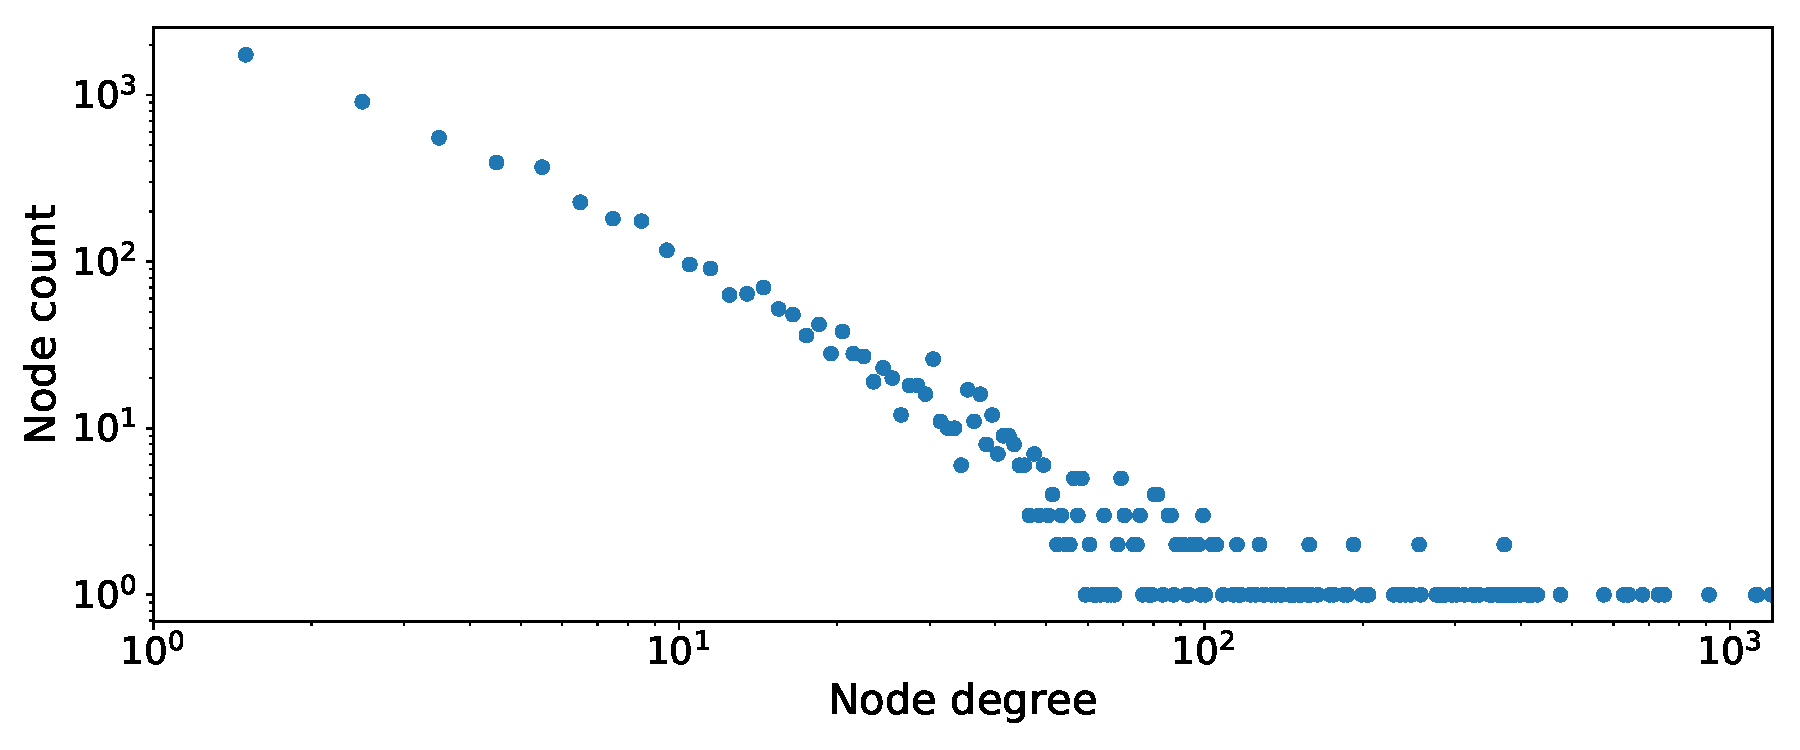
\includegraphics[width=0.8\columnwidth]{node-degree-histogram}
	\caption{Node degree distribution.}
	\label{fig:node-degree-histogram}
\end{figure}

\begin{figure}[tb]
	\centering
	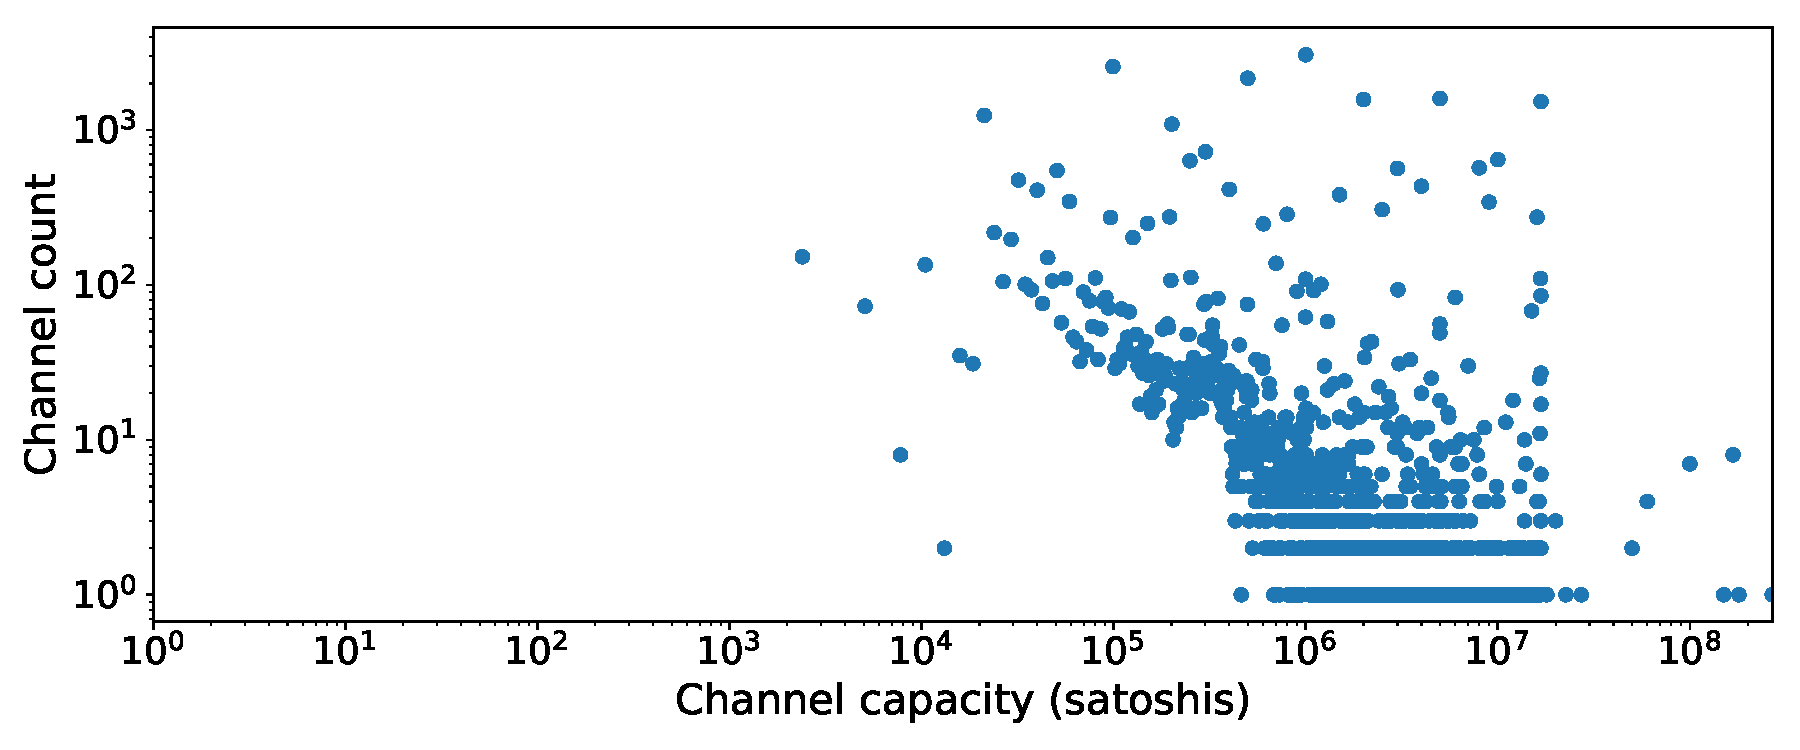
\includegraphics[width=0.8\columnwidth]{channel-capacity-histogram}
	\caption{Channel capacity distribution.}
	\label{fig:channel-capacity-histogram}
\end{figure}

\paragraph{Ethical considerations} 
Our analysis is based solely on publicly available data.
All our calculations use a local representation of the LN network graph obtained from~\cite{fiatjaf2020}.
We do not interfere with the LN activity, nor deanonymize any nodes.


\section{Security and privacy attacks: background}
\label{sec:sec-priv-attacks}

The LN builds upon hash time-locked contracts aiming to achieve atomicity in multi-hop payments.
However,~\cite{Malavolta2019} argues that due to the \emph{wormhole attack}, atomicity does not hold in LN\@.
Another study~\cite{Malavolta2017} shows that attackers can breach the privacy of LN users.
The feasibility of these attacks depends, among other factors, on the topology of the LN\@.
In this experiment, we aim to quantify the impact of these security and privacy issues on the LN\@.

\begin{figure*}[tb]
	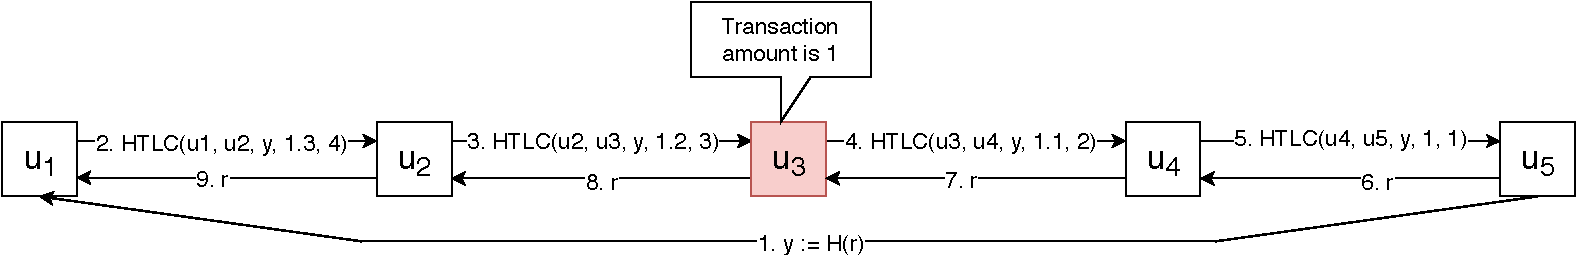
\includegraphics[width=\textwidth]{vp-figure.pdf}
	\vspace{0.3cm}
	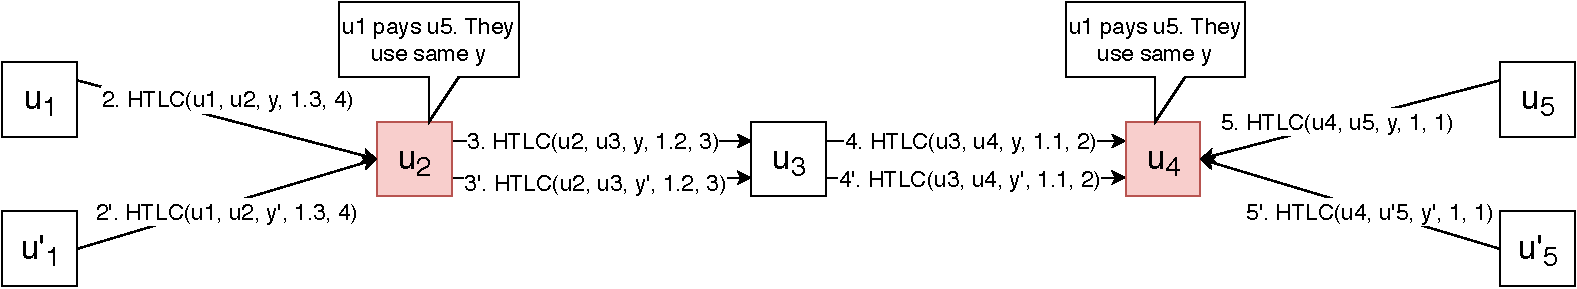
\includegraphics[width=\textwidth]{ra-figure.pdf}
	\vspace{0.3cm}
	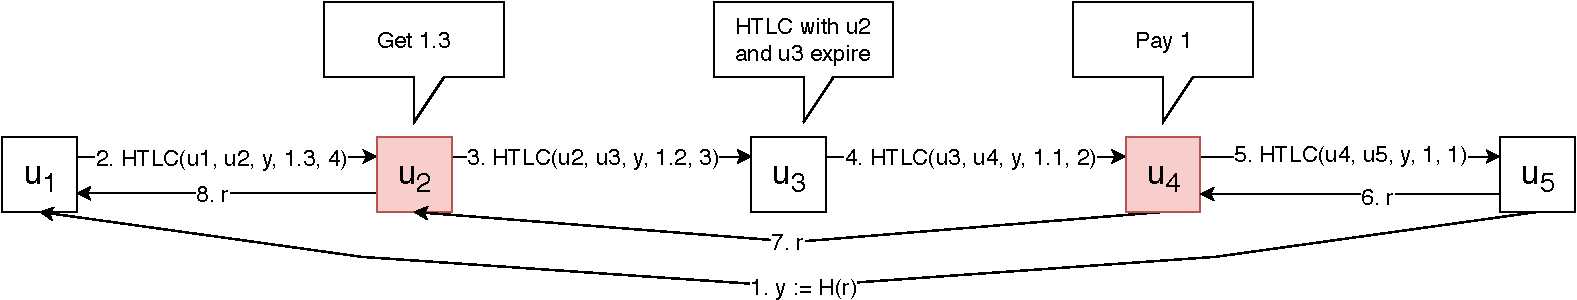
\includegraphics[width=\textwidth]{wa-figure.pdf}
	\caption{An illustrative example of value privacy (top), relationship anonymity (middle), and the wormhole attack (bottom).}
	\label{fig:wormhole-attack}
\end{figure*}

\subsubsection*{Value privacy}
Intuitively, value privacy ensures that for a payment involving only honest users, corrupted users outside the payment path learn no information about the payment value.
This notion thus heavily relies on the existence of paths without malicious nodes.
Otherwise, a malicious intermediary node can trivially learn the (upper bound of the) amount of a payment that it forwards.
For instance, in~\cref{fig:wormhole-attack} the adversary~$u_3$ forwards $1.2$~coins to~$u_4$, estimating the payment amount at around $1$~coin plus forwarding fees.

\subsubsection*{Relationship anonymity}
Intuitively, relationship anonymity ensures that given two simultaneous payments between two pairs of nodes $(u_1, u_2)$ and~$(u'_1, u'_2)$ routed through the same path of intermediary users $i_1, \ldots, i_n$, the adversary controlling some of those intermediaries cannot tell who is paying to whom with probability better than~$1/2$.
However, the LN does not achieve relationship anonymity.
An adversary controlling $i_1$ and~$i_n$ can use the cryptographic challenge included in the HTLC to determine who pays to whom.
For instance, in~\cref{fig:wormhole-attack} the adversary controlling $u_2$ and~$u_4$ can determine that $u_1$ is transacting with~$u_5$ as the same value~$y$ is used along the whole path.
Similarly, $u_2$ and~$u_4$ can determine that $u'_1$ is transacting with~$u'_5$ as the same~$y'$ is used along the path.

\subsubsection*{The wormhole attack}
In the wormhole attack, two colluding nodes in a payment path prevent honest intermediaries from participating in the payment, stealing the fees intended for honest intermediaries.
One may argue that this is not an attack, as, from the sender's point of view, the payment is delivered.
However, this attack diminishes the economic incentive for honest users to forward payments in the first place.

An example of the wormhole attack is depicted in~\cref{fig:wormhole-attack}.
Here, $u_4$ does not send the opening value~$r$ to~$u_3$ (step 7 in~\cref{fig:htlc}).
Instead, $u_4$ sends the value~$r$ to~$u_2$ outside the LN protocol, which allows $u_2$ to settle the HTLC with~$u_1$.
As a result, contracts with~$u_3$ expire, simulating payment failure, and prevent $u_3$ from participating in the payment's successful completion.


\section{Methodology}

We first compute the paths between pairs of nodes.
Given nodes $u_1$ and~$u_2$, we compute the list of paths that connect them with one restriction: we consider only the paths with at most three intermediary nodes.
We observe that these path lengths suffice to allow more than~$85\%$ of payments between a random pair of nodes (\cref{fig:payment-success}) and allow us to exemplify all attacks that we want to study in this experiment.

\begin{figure}
	\centering
	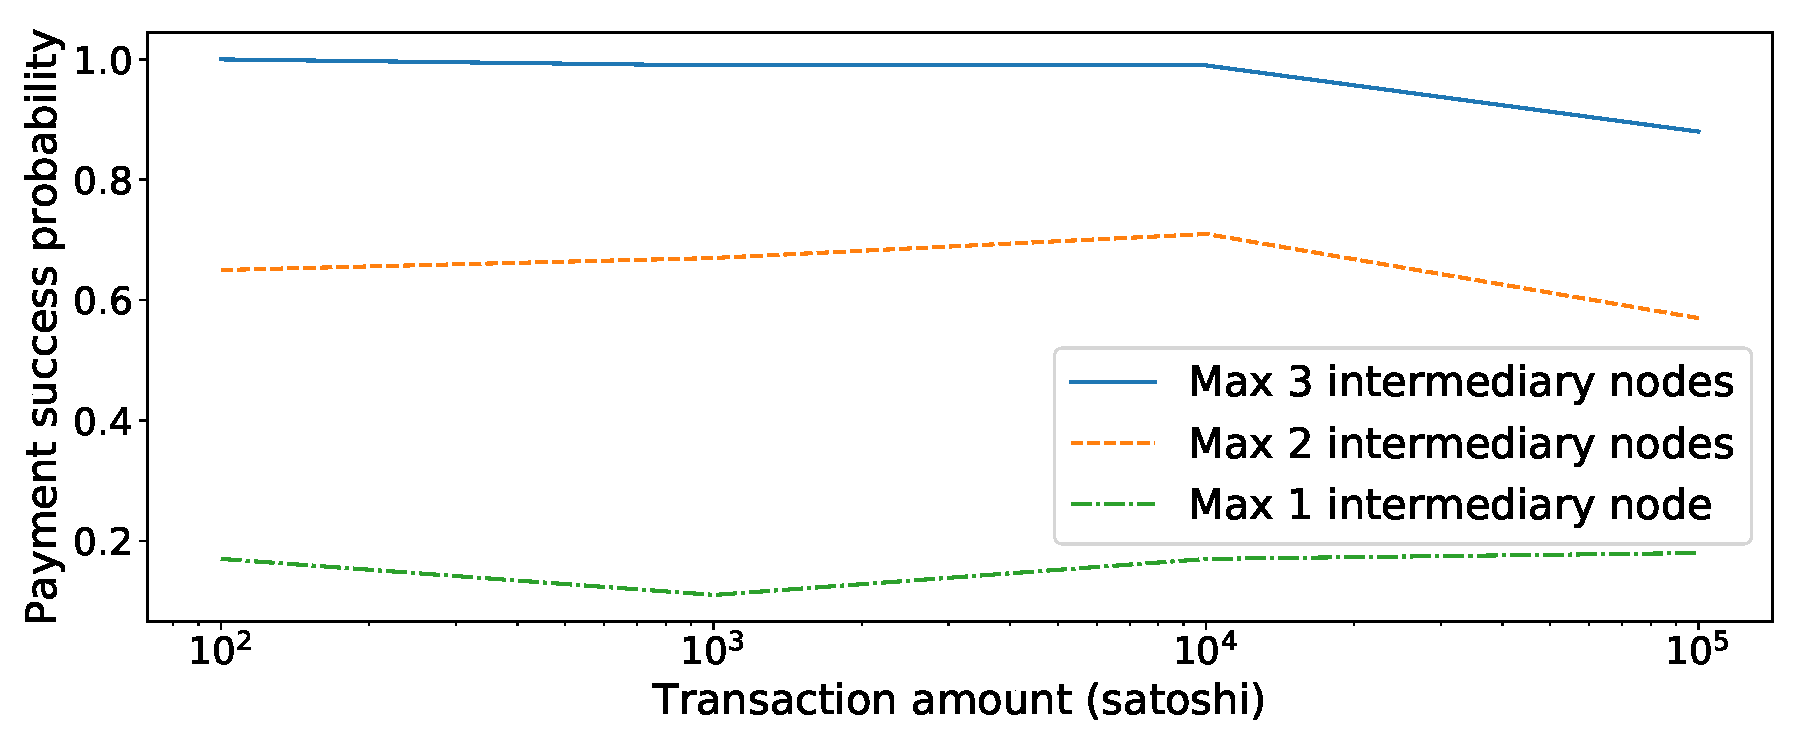
\includegraphics[width=0.8\columnwidth]{payment-success}
	\caption{The share of experiment runs where paths with sufficient capacity exist between sender and receiver.}
	\label{fig:payment-success}
\end{figure}

Let $\textit{paths}_{\langle u_1, u_2 \rangle}$ be the set of paths between $u_1$ and~$u_2$.
We prune the set $\textit{paths}_{\langle u_1, u_2 \rangle}$ into a subset $\textit{paths}_{\langle u_1, u_2 \rangle, x}$, containing only the paths that allow to transfer at least $x$~satoshis.
For instance, $\textit{paths}_{\langle u_1, u_2 \rangle, 10}$ contains the paths between $u_1$ and~$u_2$, which allows transferring at least $10$~satoshis.

For a channel to be capable of transferring $x$~satoshis from~$u_i$ to~$u_j$, $u_i$ must have a balance of at least $x$~satoshis.
However, the current balance of each counterparty in a channel is not publicly available.
Thus, we consider a path suitable for a given payment if the total capacity of every channel in the path is above the payment amount, independently of how this capacity is distributed between the counterparties.
This heuristic might consider a path suitable for a payment while it is not.
We nevertheless follow this heuristic as LN nodes also use it in practice.

As the next step, we study the effectiveness of the selected attack.
For a chosen payment amount~$x$, we split the set $\textit{paths}_{\langle u_1, u_2 \rangle, x}$ into two subsets:

\begin{enumerate}
	\item $\textit{paths-prone}_{\langle u_1, u_2 \rangle, x}$: the subset of paths prone to the attack;
	\item $\textit{paths-safe}_{\langle u_1, u_2 \rangle, x}$: the subset of paths not susceptible to being attacked.
\end{enumerate}

The definition of a path of the form~$u_1 \rightarrow i_1 \rightarrow \ldots \rightarrow i_n \rightarrow u_2$ being prone to the specific attack depends on the attack:

\begin{itemize}
	\item \textit{Value privacy}: We say that a path is prone to the value privacy attack if any intermediary node is under adversarial control.
	
	\item \textit{Relationship anonymity}: We say that a path is prone to the relationship anonymity attack if nodes $i_1$ and~$i_n$ are under adversarial control.
	
	\item \textit{Wormhole attack}: We say that a path is prone to the wormhole attack if there exist two non-neighboring intermediary nodes $i_j$ and~$i_k$  under adversarial control (i.e.,~$j < k$ and~$k \neq j + 1$).
\end{itemize}

Note the difference between the definitions of a prone path in the wormhole attack and the relationship anonymity attack.
The latter does not require an honest user to be located between the two malicious nodes.
For instance, a path of the form $u_1 \rightarrow i_1 \rightarrow i_2 \rightarrow u_2$ where $i_1$ and~$i_2$ are under adversarial control would be considered prone to the relationship anonymity attack but safe against the wormhole attack.

Another aspect that we consider is which nodes are malicious.
We follow three strategies.
First, we assume that nodes with the highest degrees (i.e.,~highly connected nodes) are colluding.
Highly connected nodes have the highest stake in the network.
Thus, an adversary might attempt to corrupt them (e.g.,~by bribery or stealing the private key) to maximize the effect of the attack.
Second, we assume that nodes with the highest total capacity in their adjacent channels are colluding.
Finally, we consider that random nodes are colluding.
We illustrate here that any node (independently of its node degree) might be corrupted.
For instance, the same user might create several LN nodes at strategic positions to carry out the attacks.

We then consider these three attack strategies.
For each number of malicious nodes ($y$) and each strategy, we re-split the set $\textit{paths-prone}_{\langle u_1, u_2 \rangle, x}$ into prone paths and safe paths.
For instance, we denote by $\textit{paths-prone}_{\langle u_1, u_2 \rangle, x, y\textit{-con}}$ the subset of paths between $u_1$ and~$u_2$ that allow to transfer $x$~satoshis and that are prone to the attack if $y$~nodes with the highest node degree are corrupted.
Correspondingly, we denote by $\textit{paths-prone}_{\langle u_1, u_2 \rangle, x, y\textit{-ran}}$ the subset of paths between $u_1$ and~$u_2$ that allow to transfer $x$~satoshis and that are prone to the attack if $y$~nodes chosen uniformly at random are corrupted.

Finally, for each attack strategy, we consider $$\alpha_{\langle u_i, u_j \rangle} := \frac{|\textit{paths-prone}_{\langle u_i, u_j \rangle, x, y}|}{|\textit{paths-prone}_{\langle u_i, u_j \rangle, x, y}| + |\textit{paths-safe}_{\langle u_i, u_j \rangle, x, y}|}$$ the probability that a payment between $u_i$ and~$u_j$ is vulnerable to the attack.
Averaging across all the pairs of nodes tested, we extract the final probabilities reported in~\cref{fig:fig-all-attacks}.

\section{Results and discussion}

\begin{figure*}
	\centering
	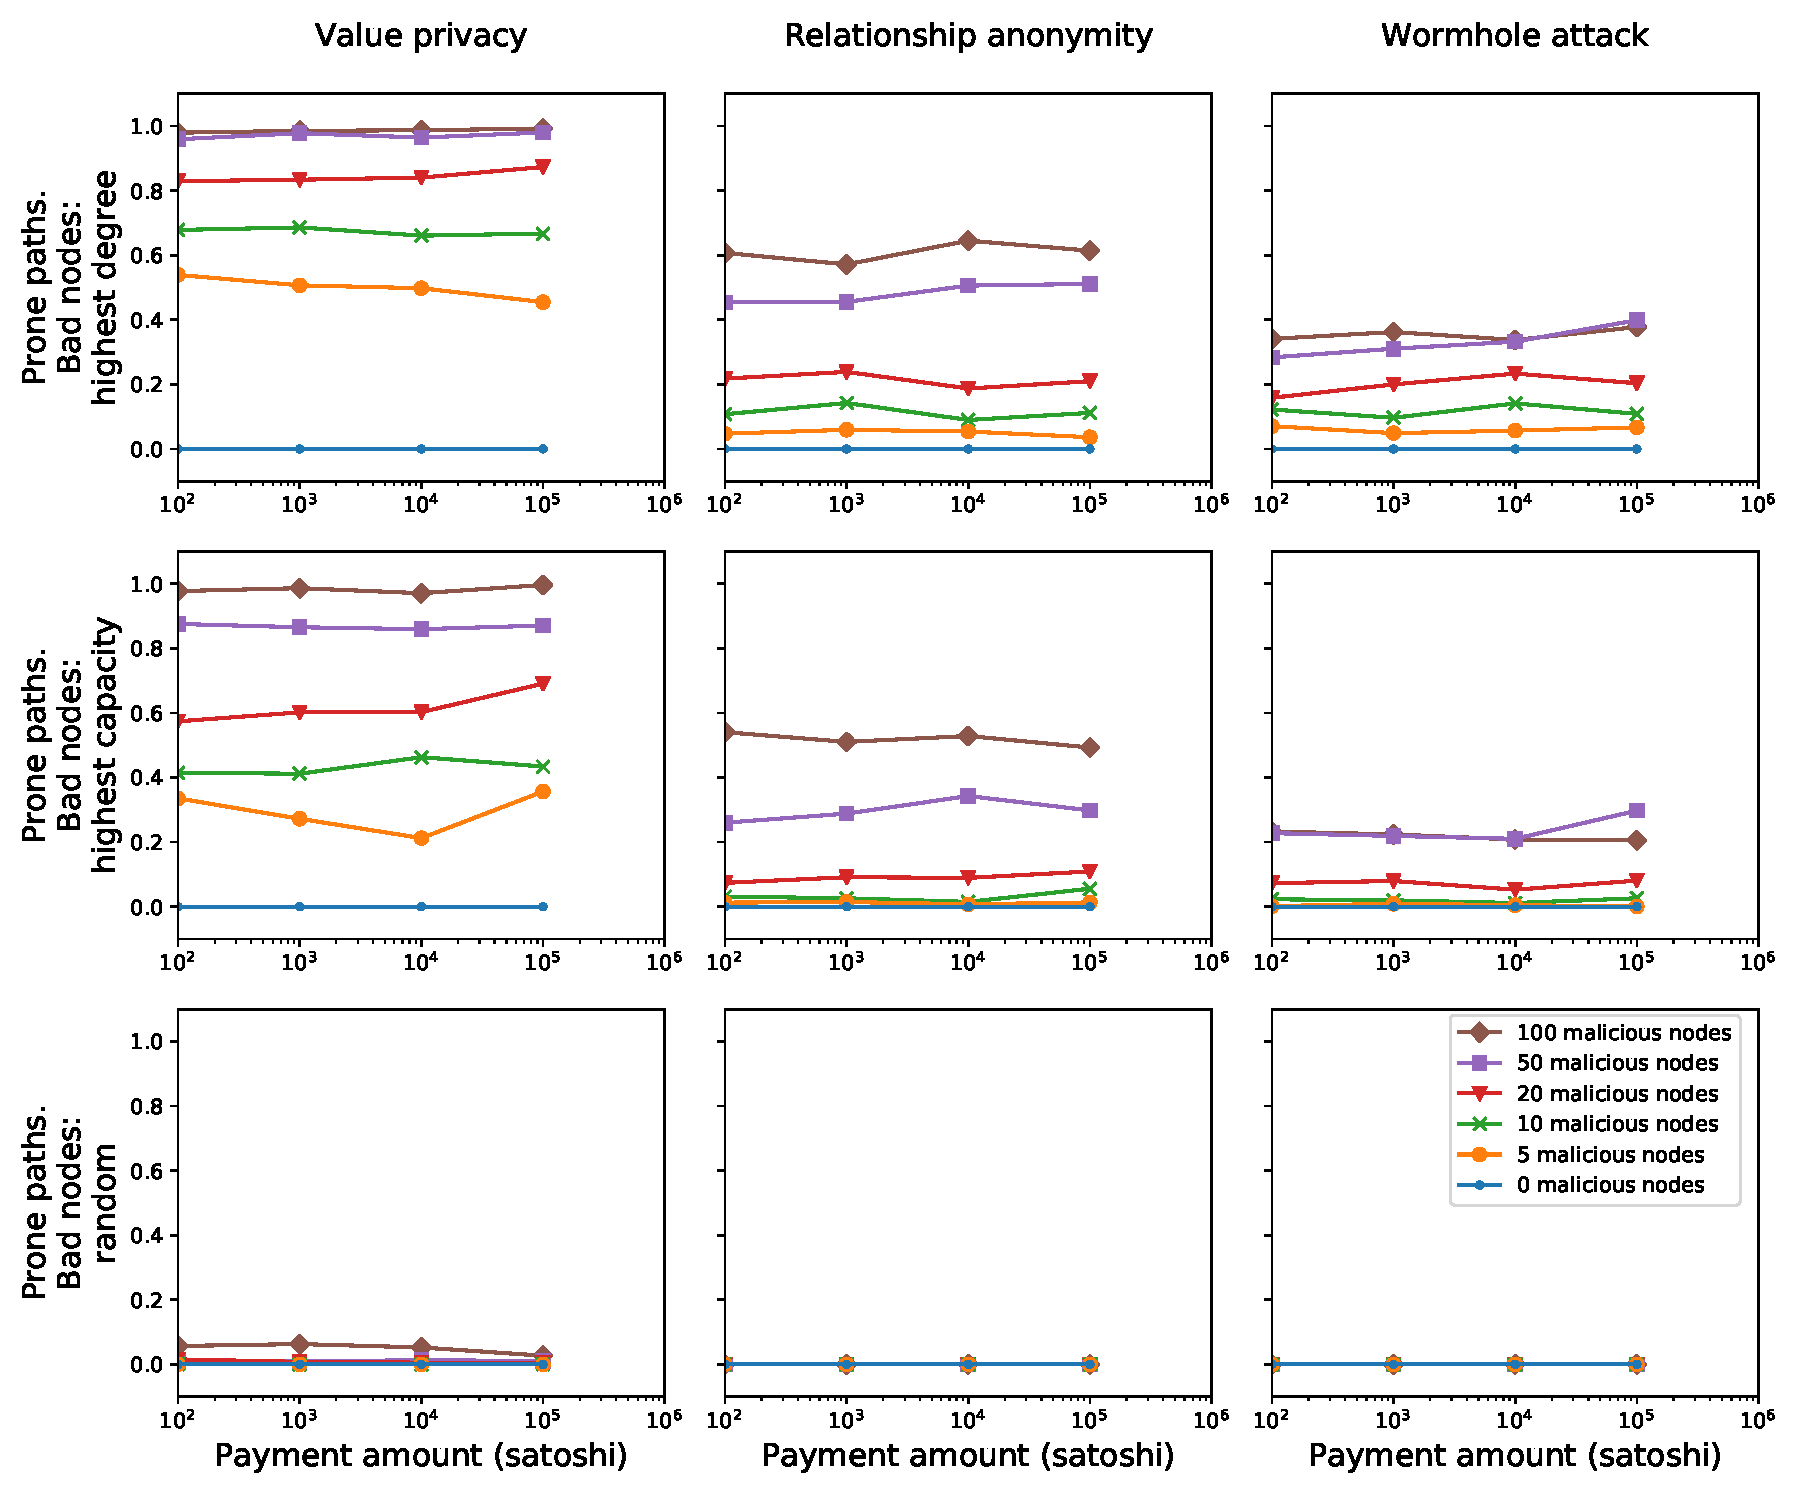
\includegraphics[width=\columnwidth]{fig-all-attacks}
	\caption{Share of prone paths for each parameter combination.}
	\label{fig:fig-all-attacks}
\end{figure*}

For every attack and a given number of compromised nodes, the share of prone paths is relatively stable for all payment amounts (\cref{fig:fig-all-attacks}).
This result indicates that the payment amount does not significantly affect the security of payments.

The three attacks differ in how quickly the share of prone paths changes as the number of compromised nodes increases.
For value privacy, the effect of added highly-connected nodes being compromised is the most profound.
The share of prone paths is $50\%$~if only the $5$~most connected nodes are compromised, and nearly $100\%$~if the $100$~most connected nodes are compromised.
Thus, we conclude that an adversary needs to corrupt only $2\%$~of the nodes to almost nullify any value privacy guarantee in the LN\@.

The average share of prone paths decreases for relationship anonymity.
However, the adversary controlling the $100$~most connected nodes can launch the relationship anonymity attack on about $70\%$~of the paths.
Interestingly, the adversary has fewer possibilities to launch the wormhole attack.
For instance, with~$100$~most connected nodes corrupted, around $30\%$~of the paths are prone to the attack.
A restrictive path structure in the definition of the attack may explain this reduction in the attack's effectiveness.

The attacker benefits less from compromising high-capacity nodes, as opposed to high-degree nodes.
This distinction is most profound for relationship anonymity: around $50\%$ of paths are vulnerable if the~$50$~highest degree nodes are corrupted, but only around~$25\%$~paths are vulnerable if the~$50$~highest capacity nodes are corrupted.
This difference may be explained by the fact that routing algorithms optimize for short paths.
Note that forwarding channels' capacity is not as important as good connectivity, especially for payments of small and medium amounts.

Finally, we consider random nodes compromised.
In contrast to the earlier results, less than $10\%$~of paths are prone to value privacy, and nearly no paths are prone to relationship anonymity and wormhole attacks.
We note that randomly selected nodes have few connections (note the degree distribution in Figure~\ref{fig:node-degree-histogram}).
Thus their compromise does not affect routing at large.

In summary, our results show that highly connected nodes and nodes with high capacity channels have a high impact on the security and privacy of the LN\@.
Assuming that paths are selected uniformly at random from the set of available paths, an adversary that selectively corrupts $100$~(i.e.,~only $2\%$) of LN nodes can effectively learn all the payment values, the sender and the receiver for most payments, and carry out the wormhole attack in about $30\%$~of the paths.
These estimations evidence that the security and privacy attacks shown in theory are indeed crucial in practice.

Carrying out such attacks might be feasible in the live network: an unknown entity under the pseudonym LNBIG is known to control $23$~out of top~$50$~highest connected nodes~\cite{1MLTopConnected} and~$40\%$~of the network capacity~\cite{TheBlockLNBIG} (as of 2019).


\section{Countermeasures}
We assume that every two nodes carry out their payments along a path chosen uniformly at random from the set of all available paths.
However, LN nodes might implement different routing strategies.
For instance, while routing through well-connected nodes improves the chances to reach the receiver through a short and highly liquid path, the sender might instead choose low degree nodes.
Routing around popular nodes may reduce the probability of choosing a compromised path.
We envision a trade-off between connectivity on the one hand and security and privacy on the other, which constitutes a direction for future work.
A node may also route payments through a trusted proxy node, thus guaranteeing that the first node in a path is not compromised.
This strategy would mitigate the relationship anonymity and wormhole attacks (if the path contains no more than three intermediaries).


\section{Conclusion}
\label{sec:conclusions}

The LN has emerged as the most widely deployed solution for scalability issues affecting current blockchains such as Bitcoin.
Despite its conceptual appeal and growing adoption, several works~\cite{Malavolta2017, Malavolta2019} have identified security, anonymity, and scalability limitations.
However, a quantitative analysis of their impact is missing, and this work aims to fill this gap.

We quantitatively study the LN's proneness to the wormhole attack and attacks against value privacy and relationship anonymity.
We observe that a moderately resourceful adversary controlling only $2\%$~of the total node count can carry out these attacks with high success probability.
As the LN evolves, the developers should acknowledge these results in future protocol design decisions.
\chapter{Throughput limitation of the Lightning network}

\label{Chapter08HTLClimit}

In this Section, we describe an inherent limitation on the number of concurrent payments Lightning channels can handle.\footnote{This Chapter is based on~\cite{Tikhomirov2020a}.}
Due to the size limitations on Bitcoin transactions, a payment channel can hold only a certain number of concurrent unresolved HTLCs.
An attacker can create unresolved payments between two nodes under their control.
This attack blocks the capacity of channels along the route by depleting their "HTLC slots."
This effect may be critical for micro-payment applications -- a significant use case for the LN.
This limitation has been pointed out~\cite{EmelyanenkoK2017} but never quantitatively analyzed.

We study the management of concurrent payments in the LN and quantify its negative effect on scalability.
We observe that for micropayments, the forwarding capability of up to $50\%$~of channels is under-utilized.
This phenomenon not only hinders scalability but also opens the door for DoS attacks.
We estimate that a network-wide DoS attack costs within $1.5M$~USD, while isolating the biggest community from the rest of the network costs only $225k$~USD\@.
We also evaluate the evolution of this phenomenon over the two years of LN existence, based on the historical data.
We finally discuss potential countermeasures.


\section{Background} \label{max-htlc-background}

Bitcoin~Core imposes a $100$~KB transaction size limit~\cite{StandardTxBitcoinSE, BitcoinCoreMaxTxWeight}.
More precisely, transaction size is one of the requirements for a \textit{standard} transaction.
Bitcoin~Core nodes, which make up $97\%$~of the network~\cite{CoinDance}, do not propagate non-standard transactions, which are therefore unlikely to get confirmed.
An LN channel cannot contain more than $966$~unsettled HTLCs~\cite{BOLT2Rationale}.
This limit ensures that both counterparties can close the channel using one standard Bitcoin transaction.
We call this limitation the \textit{HTLC limit}.

Despite the perceived focus on micropayments, LN does not fully support transactions of very small value.
Every HTLC increases the weight of a potential closing transaction and therefore increases the on-chain fees.
Redeeming very small outputs on-chain can be more expensive than their value.
Therefore, BOLT specifications prescribe that nodes negotiate the \textit{dust limit} before opening a channel.
Nodes do not create HTLCs for payments below this limit.
Such non-existent outputs are called \textit{trimmed HTLCs}~\cite{BOLT3Trimmed}.
Out of the three most popular LN implementations, c-lightning and Eclair use the default dust limit of~$546$~satoshis.
LND estimates the dust limit dynamically based on the current on-chain fees.
We thus assume $546$~satoshis as the dust limit.


\section{The HTLC limit effect on LN scalability}

This section estimates the effect of the HTLC limit on the number of concurrent channel updates.
We use the same dataset \textit{LN20} as in Chapter~\ref{Chapter07LNattacks}.
We derive a series of historical snapshots representing the state of the LN on the first day of each month from April~2018 to February~2020.
We refer to this dataset as \textit{LNHist}.

Let $C$ be the total network capacity (i.e., the sum of all channels' capacities).
We only consider amounts above the dust limit $D$.
Let $a_\textit{avg}$ be the average transaction amount.
We define the limit on concurrent updates based solely on capacity as $u_\textit{cap} := C / a_\textit{avg}$.
In contrast, the limit on concurrent updates considering the HTLC limit is $u_\textit{HTLC} = N * 966$, where $N$ is the number of channels.
We remark here that $u_\textit{HTLC}$ does not depend on transaction amounts.

Given those two values, we define the \textit{effective update rate} $ur_\textit{eff}$ as the ratio between the actual limit on concurrent transactions considering the HTLC limit and the theoretical limit based solely on capacity:

\[ur_\textit{eff} = \frac{min(u_\textit{cap}, u_\textit{HTLC})}{u_\textit{cap}}\]

Note that the effective update rate $ur_\textit{eff}$ depends on the average transaction amount, as shown in Figure~\ref{fig:effective-channel-updates}.
Starting from $D$, the effective number of concurrent updates diverges from what could be theoretically possible without the HTLC limit.
We observe that $2\,677$~satoshis ($0.24$~USD) is the \textit{borderline amount}: for higher average transaction amounts, the limiting factor for the number of concurrent channel updates is channel capacity.
For amounts between $D$~and~$2\,677$~satoshis, the limiting factor is the HTLC limit.

\begin{figure}[tb]
	\centering
	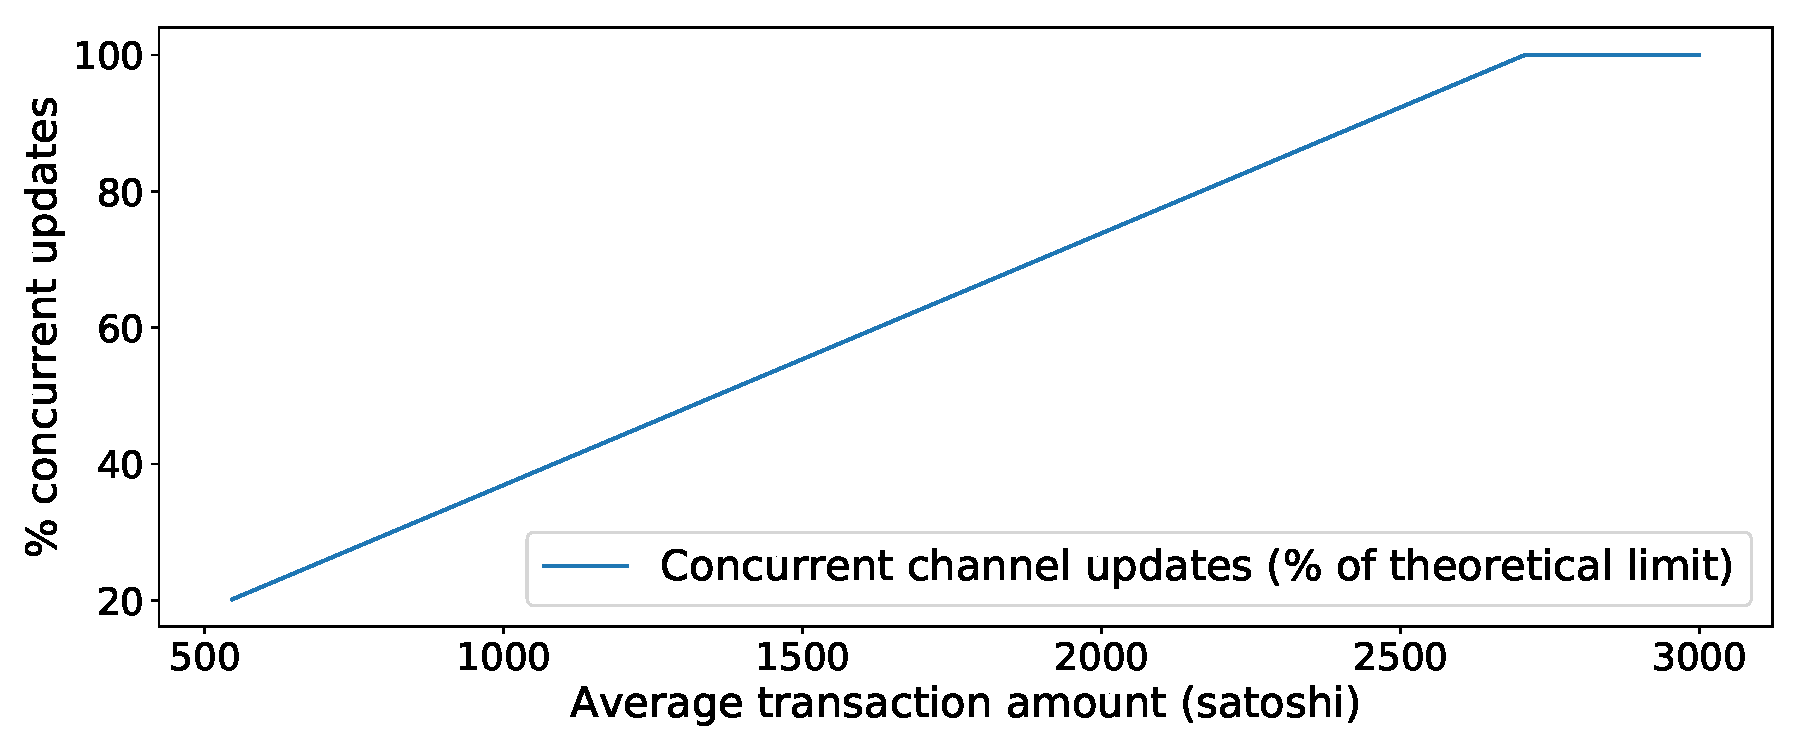
\includegraphics[width=0.8\columnwidth]{effective-channel-updates}
	\caption{Ratio between the current limit on concurrent channel updates and the theoretically possible capacity-based limit.}
	\label{fig:effective-channel-updates}
\end{figure}

\paragraph{Affected channels}
The $ur_\textit{eff}$ is an aggregated measurement that does not shed light on how the HTLC limit affects individual channels. 
We now study how many channels are affected by the HTLC limit.
The number of affected channels depends on the average transaction amount $a_\textit{avg}$.
For high values of~$a_\textit{avg}$, it is more likely that the channel's capacity limits its effective update rate, whereas the HTLC limit determines the update rate cap for small values of~$a_\textit{avg}$.
We quantify this as follows.
Given a fixed average transaction amount $a_\textit{avg}$, we consider a channel \textit{affected} by the HTLC limit if $u_{\textit{HTLC},a_\textit{avg}} < u_{\textit{cap},a_\textit{avg}}$, i.e, $u_{\textit{eff},a_\textit{avg}} < 100\%$~(\cref{fig:affected-channels}).

\begin{figure}[tb]
	\centering
	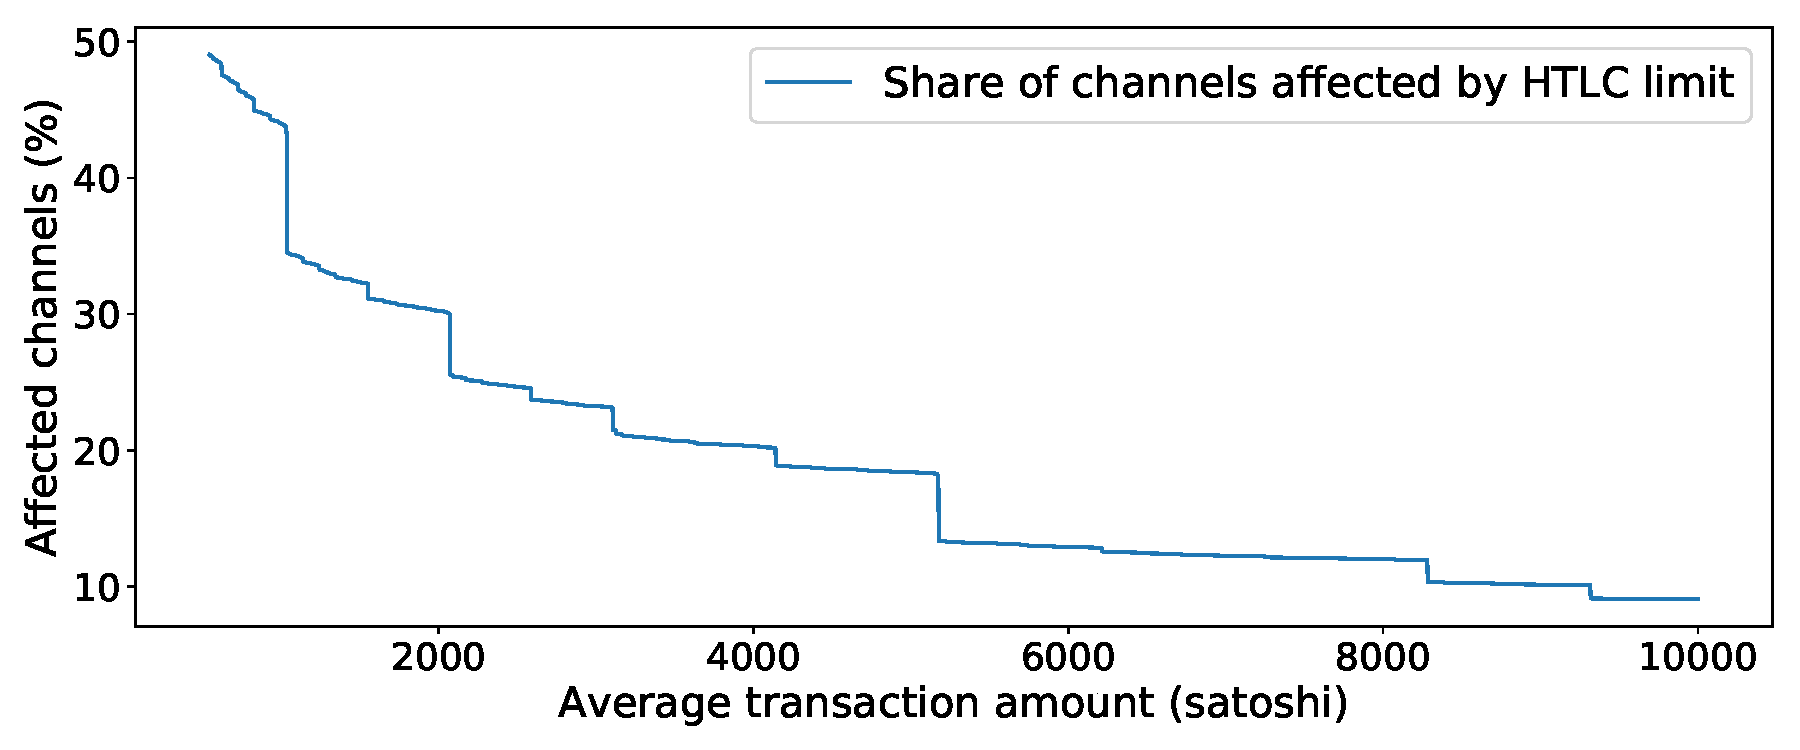
\includegraphics[width=0.8\columnwidth]{affected-channels}
	\caption{Share of affected channels for different transaction amounts.}
	\label{fig:affected-channels}
\end{figure}


\paragraph{The effect of the HTLC limit over time}

We study the effect of the HTLC limit on the LN using our historical snapshots \emph{LNHist}.
For each monthly snapshot and four assumed average transaction amounts, we calculate the share of channels affected by the HTLC limit (\cref{fig:historic-htlc-limited-share}).
As expected, the HTLC limit becomes a more pressing issue with smaller transaction amounts, if they are above the dust limit.
We also observe that the share of affected channels has been increasing in the early months of the LN's existence and has remained stable since mid-2019.

We finally study how the \textit{borderline amount} has changed over time.
As~\cref{fig:historic-borderline-amount} shows, the HTLC limit finds its inflection point in transaction amount at approximately $2\,500$~satoshis, with the borderline amount stabilizing in mid-2019, after the initial growth.

\begin{figure}[tb]
	\centering
	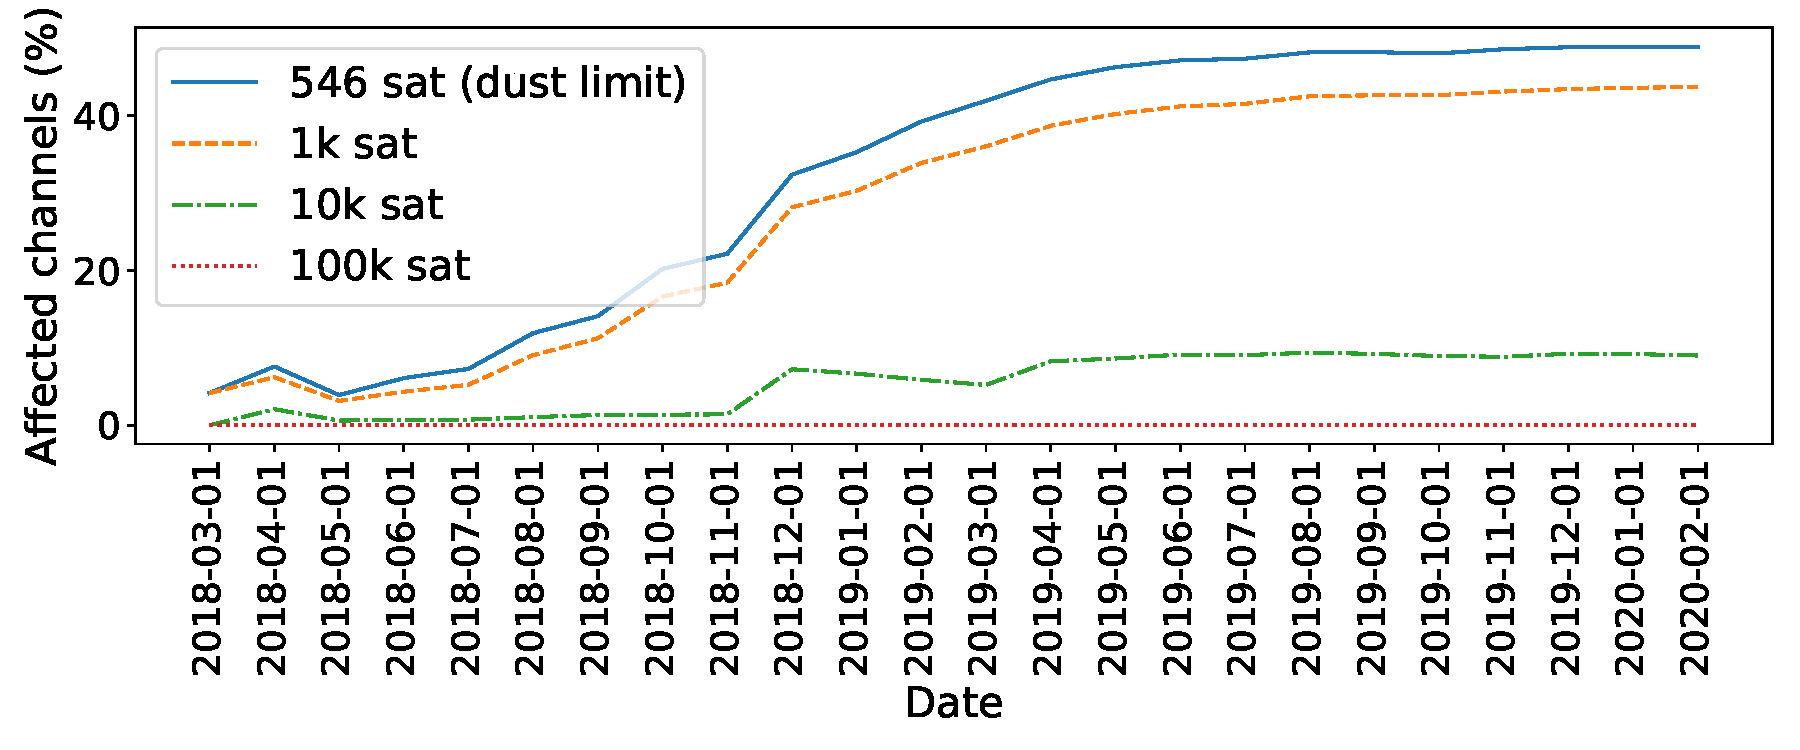
\includegraphics[width=0.8\columnwidth]{historic-htlc-limited-share}
	\caption{Historic share of HTLC-limited channels.}
	\label{fig:historic-htlc-limited-share}
\end{figure}

\begin{figure}[tb]
	\centering
	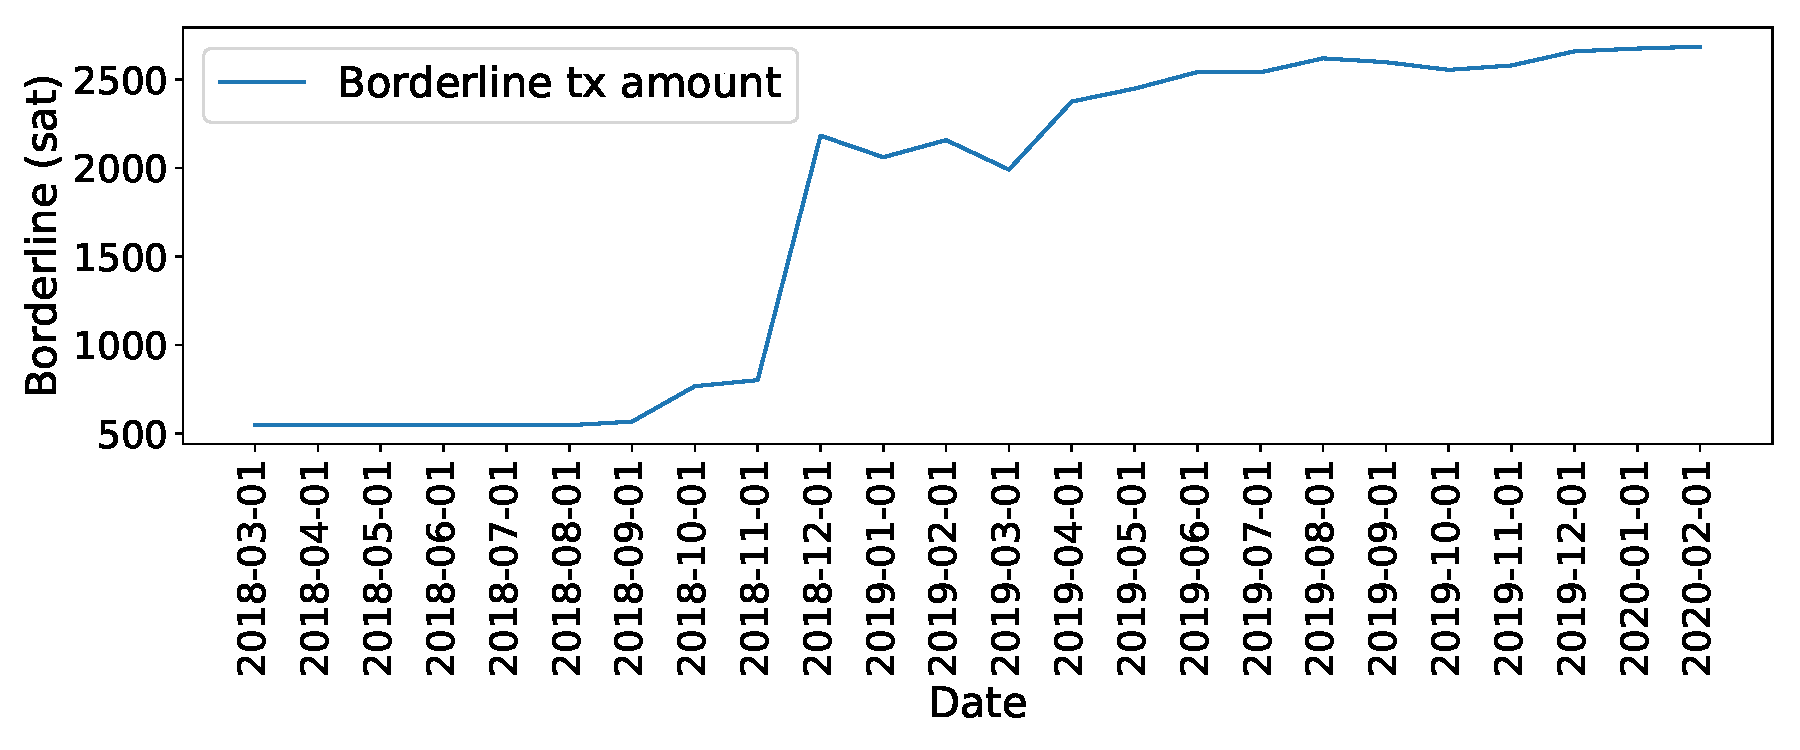
\includegraphics[width=0.8\columnwidth]{historic-borderline-amount}
	\caption{Historic borderline amounts.}
	\label{fig:historic-borderline-amount}
\end{figure}


\section{Depleting the Lightning Network}

The HTLC limit enables a network-wide DoS attack.
An adversary connects to both endpoints of the target channel and forwards multiple small payments to itself, but does not finalize them.
After $966$~HTLCs are added, the channel loses its ability to forward payments until some HTLCs expire.
The attacker can thereby deplete a channel, making it unusable.

The cost of this attack depends on the minimum transaction amount.
We assume it equal to the dust limit of~$546$~satoshis (the default value in 2 out of 3 major LN implementations).

We calculate the total capital requirements for an attacker to block the LN completely.
To block all $31\,084$~channels, the attacker would send, in the worst case, $966$~transactions of~$546$~satoshi to each channel.
This brings the total capital requirements to approximately $163.9482$~BTC ($1.64M$~USD).

Each HTLC defines a timeout, after which the funds are returned to the sender if the receiver provides no preimage.
From our dataset, we see that HTLC timeouts are long: $75.44$~blocks on average.
At a block creation rate of~$10$~minutes per block, this implies that an average HTLC can block the capacity for around $12$~hours.
Therefore, the attacker can render channels useless for around $12$~hours using the same HTLC parameters as regular LN users.

While this rough upper bound estimate suggests a relatively high attack cost, the following optimizations make it more affordable.


\paragraph{Targeting highest-capacity channels}
The attack impact can be maximized by targeting the highest-capacity channels.
For example, it requires $0.05$~BTC to block 10~top channels with combined capacity of~$17.91$~BTC (\cref{fig:block-top-channels}).

\begin{figure}[tb]
	\centering
	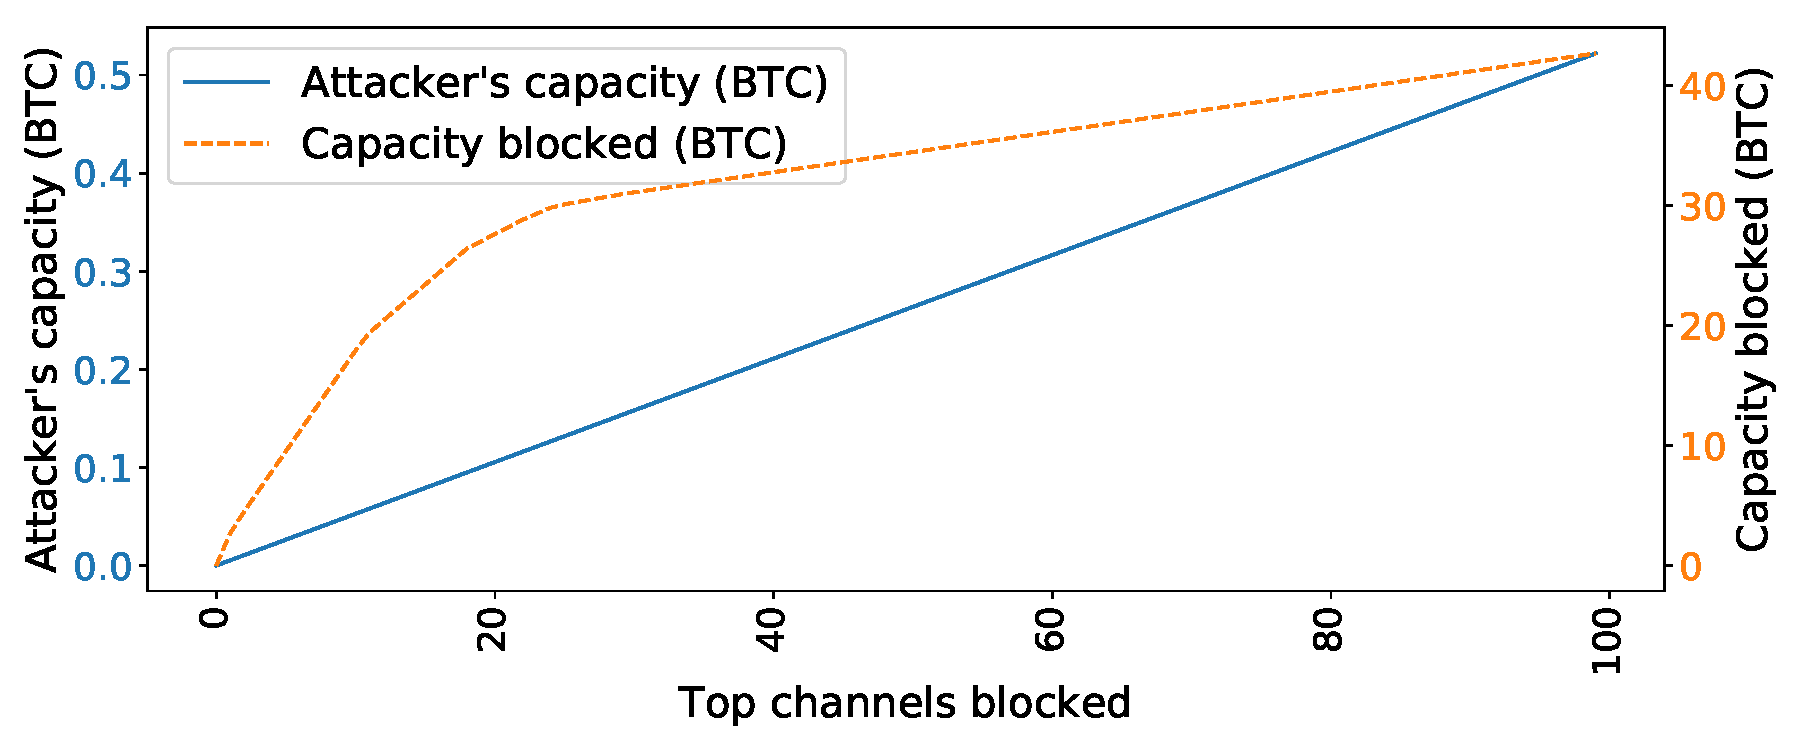
\includegraphics[width=0.8\columnwidth]{block-top-channels}
	\caption{Effectiveness of targeting highest-capacity channels.}
	\label{fig:block-top-channels}
\end{figure}

\paragraph{Real HTLC limit}
Our calculations are based on the maximum number of concurrent HTLCs ($483$) as defined by BOLT specifications.
LN implementations may choose other values.
In particular, Eclair and c-lightning enforce a lower default HTLC limit ($30$).
Lower limits mean that in the real network, the attacker would need to create fewer HTLCs to block channels between c-lightning and Eclair nodes than between LND nodes (which by default support $483$~concurrent HTLCs per channel).
LND makes up $91\%$~of the nodes in the network, and Eclair is another $1\%$~\cite{Mizrahi2020}.
That brings the real average HTLC limit to $442.23$~and lowers the attack cost by~$8.44\%$.

\paragraph{Multi-hop transactions}
Our estimation assumes single-hop transactions.
An attacker can leverage multi-hop transactions to multiply the effect of the committed capital, connecting to both ends of a $20$-hop~\cite{Bolt4OnionRouting} payment path and performing a payment to itself that never gets completed.
This technique resembles capacity-based griefing attacks~\cite{HerreraJoancomarti2019} but entails much lower capital requirements.

\paragraph{Optimizing the attack based on communities}
The attacker may wish to prevent different parts of the network from transacting to each other.
To evaluate this possibility, we first divide the network into \textit{communities} using the Clauset-Newman-Moore greedy modularity maximization algorithm~\cite{Clauset2004}.
Then we consider a scenario where the attacker tries to block the channels that connect communities rather than channels within communities.
For a chosen number $N$~of the largest communities, we calculate how many channels the attacker has to block to split the network into at least $N+1$~parts: the $N$~largest communities and the rest of the network (\cref{fig:isolate-communities}).
We infer, e.g.,~that the attacker needs to block $4\,670$~channels ($13\%$~of all channels) to isolate the largest community from the rest of the network, locking up $25$~BTC ($225k$~USD) -- or around $2.8\%$~of the total LN capacity.

\begin{figure}[tb]
	\centering
	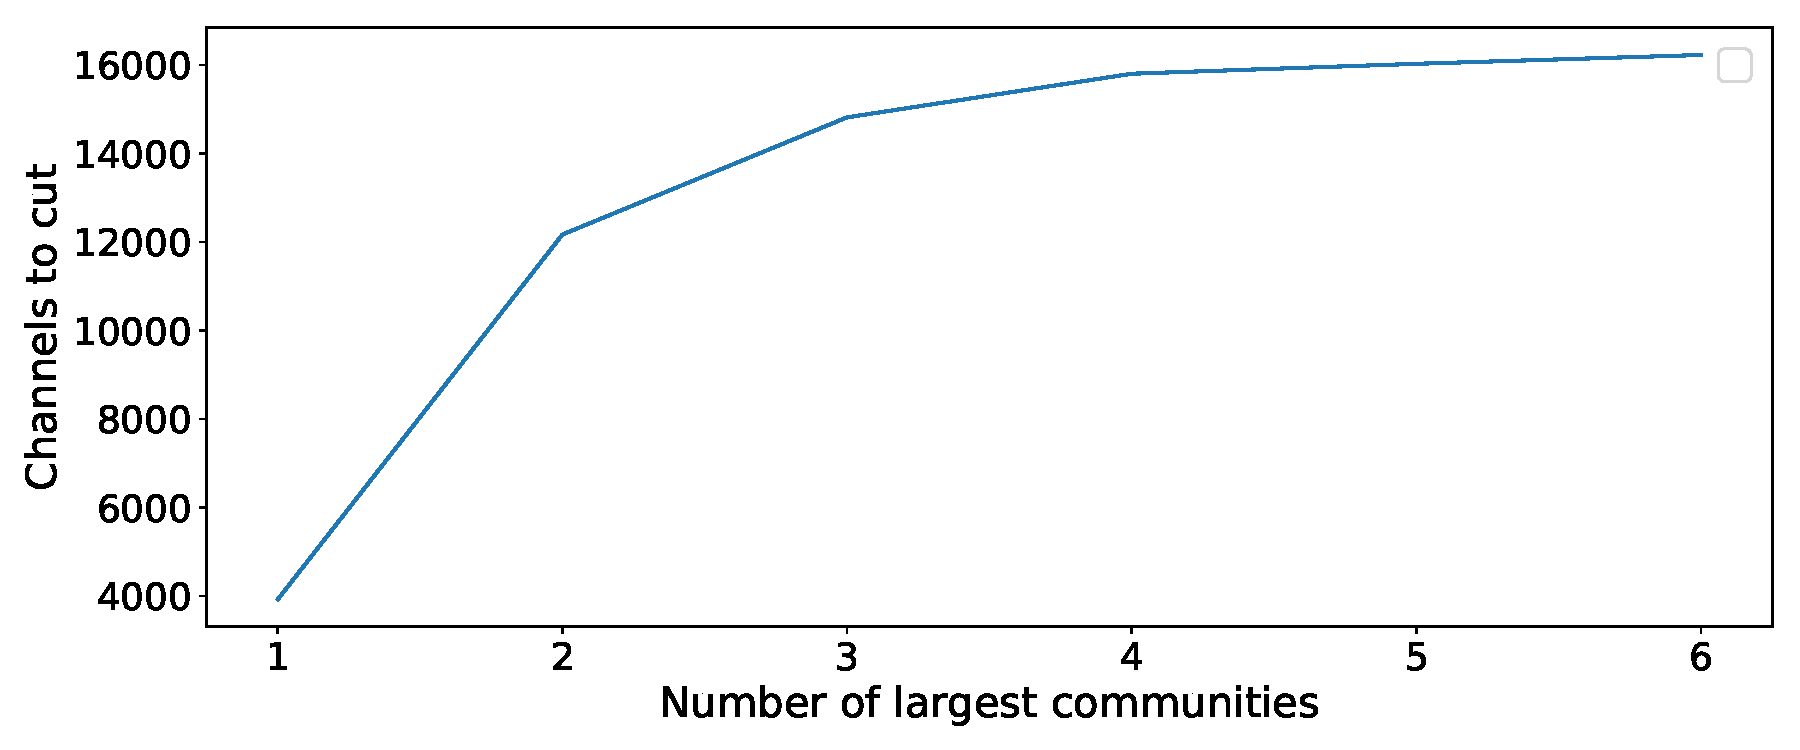
\includegraphics[width=0.8\columnwidth]{isolate-communities}
	\caption{Number of channels to cut to isolate the largest communities.}
	\label{fig:isolate-communities}
\end{figure}


\section{Discussion}
Our simplistic model does not fully reflect all the details of transaction handling.
In particular, we do not account for multi-hop transactions and transactions that try multiple paths before succeeding.
We do not reflect the unequal forwarding ability of a unit of capacity at a well-connected node, as opposed to a poorly connected one.
We also do not account for non-public channels, which may account for $28\%$~of all channels~\cite{BitMEXPrivateChannels}.
Nevertheless, our approach allows us to calculate the effect of the HTLC limit, as we derive both estimations (capacity-based limit and HTLC limit)  under the same assumptions.

The negative effect of the HTLC limit manifests itself at low transaction amounts.
This threatens some potential LN applications involving micro-payments, such as paying for online content~\cite{Poon2016}.
Our calculations show that for payments of~$1\,000$~satoshis ($0.009$~USD), the network-wide rate of concurrent channel updates is $60\%$~lower than it could have been based solely on capacity limitations.

The low value for the default minimum transaction amount and the reduced number of in-flight transactions open a DoS attack vector with a moderate cost for the adversary.
Note that the capital in the attacker's channels will be recouped after the HTLCs time out.
Moreover, the unequal distribution of connectivity in the current LN paves the way for optimized attacks where the attacker focuses on high-capacity or inter-community channels to disrupt the transfer of value across the network.


\section{Countermeasures}
One of the limiting factors for transaction throughput is the total available capacity.
This limitation is overcome by opening new channels, a countermeasure naturally implemented with the growing LN adoption.
The HTLC limit issue is more challenging as it comes from the limitations of the Bitcoin and Lightning protocols themselves.
Therefore, more fundamental changes are needed to reduce the information required to carry out the functionality encoded in HTLCs.
One countermeasure involves replacing HTLCs with atomic multi-hop locks (AMHL)~\cite{Malavolta2019}.
While an HTLC requires a digital signature, hash value, and a timelock, AMHL only requires a digital signature and a timelock while providing the same functionality.
This countermeasure would reduce the number of bytes required per in-flight transaction and increase the number of payments handled concurrently.
While not removing the limitation on the number of concurrent transactions, this countermeasure raises this limit, reducing its harmful effect.


\section{Conclusion}

We have quantitatively analyzed the negative effect on scalability produced by the limit on concurrent payments in the LN\@.
The LN's limited concurrency implies that an adversary can block the complete network investing around $1.5M$~USD ($18.5\%$~of the network capacity).
In comparison to~\cite{PerezSola2019}, our HTLC depletion attack achieves the same result (a victim node can not forward payments) but exploits the HTLC limit at each channel rather than its capacity.
Compared to~\cite{Mizrahi2020}, we properly account for the way LN handles payments below the dust limit.
The attack cost can be substantially reduced by targeting highly valuable channels (e.g., high-capacity channels or those connecting the network's largest communities).


\part{Security of smart contracts on Ethereum}
%\usepackage{listings, xcolor}

\definecolor{verylightgray}{rgb}{.97,.97,.97}

\lstdefinelanguage{Solidity}{
	keywords=[1]{anonymous, assembly, assert, balance, break, call, callcode, case, catch, class, constant, continue, contract, debugger, default, delegatecall, delete, do, else, event, export, external, false, finally, for, function, gas, if, implements, import, in, indexed, instanceof, interface, internal, is, length, library, log0, log1, log2, log3, log4, memory, modifier, new, payable, pragma, private, protected, public, pure, push, require, return, returns, revert, selfdestruct, send, storage, struct, suicide, super, switch, then, this, throw, transfer, true, try, typeof, using, value, view, while, with, addmod, ecrecover, keccak256, mulmod, ripemd160, sha256, sha3}, % generic keywords including crypto operations
	keywordstyle=[1]\color{blue}\bfseries,
	keywords=[2]{address, bool, byte, bytes, bytes1, bytes2, bytes3, bytes4, bytes5, bytes6, bytes7, bytes8, bytes9, bytes10, bytes11, bytes12, bytes13, bytes14, bytes15, bytes16, bytes17, bytes18, bytes19, bytes20, bytes21, bytes22, bytes23, bytes24, bytes25, bytes26, bytes27, bytes28, bytes29, bytes30, bytes31, bytes32, enum, int, int8, int16, int24, int32, int40, int48, int56, int64, int72, int80, int88, int96, int104, int112, int120, int128, int136, int144, int152, int160, int168, int176, int184, int192, int200, int208, int216, int224, int232, int240, int248, int256, mapping, string, uint, uint8, uint16, uint24, uint32, uint40, uint48, uint56, uint64, uint72, uint80, uint88, uint96, uint104, uint112, uint120, uint128, uint136, uint144, uint152, uint160, uint168, uint176, uint184, uint192, uint200, uint208, uint216, uint224, uint232, uint240, uint248, uint256, var, void, ether, finney, szabo, wei, days, hours, minutes, seconds, weeks, years},	% types; money and time units
	keywordstyle=[2]\color{teal}\bfseries,
	keywords=[3]{block, blockhash, coinbase, difficulty, gaslimit, number, timestamp, msg, data, gas, sender, sig, value, now, tx, gasprice, origin},	% environment variables
	keywordstyle=[3]\color{violet}\bfseries,
	identifierstyle=\color{black},
	sensitive=false,
	comment=[l]{//},
	morecomment=[s]{/*}{*/},
	commentstyle=\color{gray}\ttfamily,
	stringstyle=\color{red}\ttfamily,
	morestring=[b]',
	morestring=[b]"
}

\lstset{
	language=Solidity,
	backgroundcolor=\color{verylightgray},
	extendedchars=true,
	basicstyle=\footnotesize\ttfamily,
	showstringspaces=false,
	showspaces=false,
	%numbers=left,		% comment this do disable line numbers
	numberstyle=\footnotesize,
	numbersep=9pt,
	tabsize=2,
	breaklines=true,
	showtabs=false,
	captionpos=b
}
\chapter{Introduction to smart contracts}

\label{Chapter09Introcontracts}

In this Chapter, we provide an introduction to smart contracts and Ethereum.\footnote{This Chapter is partially based on~\cite{Tikhomirov2017}.}
We describe the history of the concept of smart contracts and its implementation in blockchain networks.
We then provide the necessary technical background on Ethereum -- a blockchain-based smart contract platform -- and outline the security and privacy challenges it faces.


\section{History of smart contracts}

A contract is a basic building block of market economy.
The foundational mechanics of a contract has not changed in centuries.
It is usually a written text designed to be interpreted by humans.

Contracts face major challenges in the digital era.
First, contacts are becoming more complex.
It is hard for humans to keep up with the speed and complexity of international finance.
Second, contracts must be enforced.
Usually, the government assumes the responsibility for contract enforcement.
However, this introduces challenges in the global Internet.


\subsection{Early ideas}

Nick Szabo coined the term \textit{smart contract} in a 1997 essay~\cite{Szabo1997}.
He argued that "contractual clauses \textelp{} can be embedded in the hardware and software \textelp{} to make breach of contract expensive".
A vending machine exemplifies a primitive smart contract.
The machine receives cash and dispenses goods and change according to the listed price.
The physical properties of the machine make attacking it sufficiently expensive to be unprofitable.

A vending machine contract is automated but still requires trust.
Moreover, the administrator has privileged access to the money and goods in the machine.


\subsection{Smart contracts in Bitcoin}

The idea of digital smart contracts remained dormant until the introduction of Bitcoin.
Bitcoin, for the first time, enabled \textit{trustless} digital contracts.
The coins can only be unlocked by providing the required arguments to their respective output scripts.
Not only do Bitcoin scripts execute as programmed, but every user can independently verify this.
Therefore, after a contract is created, users no longer have to trust the administrator.

This key property of Bitcoin lead to the first attempts at encoding complex contracts in Bitcoin outputs.
Early Bitcoin-based protocols towards this goal include Colored Coins~\cite{Rosenfeld2012}, Counterparty~\cite{Counterparty, Bartoletti2017a}, and Mastercoin~\cite{Willett2016}.

Bitcoin's programming capabilities are too restrictive to encode many types of contracts.
First, Bitcoin script is not Turing-complete.
It means, for instance, that it does not support loops.
Second, Bitcoin contracts lack the ability to access other contracts.
Each transaction is executed in isolation and can either be deemed valid or not.
It is impossible to branch depending on the results of executing another transaction.
On the one hand, such limitations limit the potential attack surface and simplify security analysis.
On the other hand, they make implementing many types of contracts difficult, if not impossible~\cite{Miller2019}.


\subsection{Smart contracts in Ethereum}

Ethereum is a blockchain platform that aims to address these limitations.
It was announced in 2014~\cite{Buterin2014, Wood2014} and launched in 2015.

Ethereum differs from Bitcoin in three major ways.

First, Ethereum provides a richer programming environment.
An Ethereum smart contract is written in a Turing-complete programming language and stored at a unique address.
Contracts can be \textit{called} by users or by other contracts.
Each transaction can have more complex effects than moving cryptocurrency units, such as changing state variables.
%In contrast, the result of a Bitcoin transaction is binary: either the UTXOs are spent or not.
This interoperability allows for composing contracts.

Second, Ethereum has updatable and addressable \textit{storage}.
Ethereum maintains consensus on the \textit{state} of all accounts.
This allows for storing arbitrary data related to contract execution on-chain.

Third, Ethereum implements an account-based model, as opposed to Bitcoin's UTXO-based model.
This simplifies the contract logic.
For instance, an Ethereum node can perform a single lookup to find out the current balance of an address, instead of scanning its whole history.

Bitcoin and Ethereum represent different points in the blockchain design space.
The differences between these two dominant open blockchain networks are often a subject of heated debate.
Some proponents of Bitcoin are eager to point out the questionable architectural decisions in the core Ethereum protocol and the vulnerabilities discovered in Ethereum smart contracts.
Members of the Ethereum community emphasize a faster evolution of Ethereum and a wider range of applications it enables.

Simple systems are usually more secure than complex ones.
The more interactions parts of the system engage in, the more things can potentially go wrong or be purposefully exploited.
The rich programming environment of Ethereum leaves more possibilities for programmers to make mistakes.
Indeed, multiple high-profile smart contracts have been hacked, losing tens of millions of~US~dollars.
These unfortunate events have shown that secure programming practices are crucial for smart contracts.


\section{Ethereum architecture}

We now provide a short introduction to the architecture of Ethereum.

\subsection{Accounts}

Ethereum can be thought of as a state machine.
Ethereum nodes communicate through a peer-to-peer network and maintain a shared view of the global state.
The state reflects the state of all \textit{accounts}.
It maps account \textit{addresses} to account \textit{states}.

Accounts in Ethereum belong to one of two types: externally owned accounts and contract accounts.
An \textit{externally owned account} is controlled by a private key.
A \textit{contract account} is controlled by a \textit{smart contract}.
Each account has a \textit{balance} and a \textit{nonce}.
The balance is the amount of the native cryptocurrency \textit{ether} controlled by this account.
Internally, balances are expressed in \textit{wei} -- the smallest denomination of ether.\footnote{$1$~ether = $10^{18}$~wei.}
The nonce is a counter that keeps track of the number of transactions issued from the account, preventing replay attacks.

Apart from balance, contract accounts have \textit{code} and \textit{storage}.
Contract code is a piece of bytecode for the Ethereum virtual machine (EVM).
Contract storage is a mapping of arbitrary variable names to their values.
The contract code controls the changes to the balance and storage of the account.\footnote{The balance of any account can also be increased by mining or by transferring the balance of another contract being destroyed with the \texttt{selfdestruct} operation.}
Internally, account data is stored in Merkle Patricia trees -- radix trees with~$256$-bit keys~\cite{MPTSpec, Buchman14}.
% The storage of a contract account can be modified (if allowed by its code), but the code itself cannot.
% "one can use create2 to deploy different bytecode to the same contract: deploy code1 - selfdestruct - deploy code2 - ..."


\subsection{Transactions}

Users interact with Ethereum by issuing \textit{transactions}.
A transaction represents a proposed state transition.

A transaction includes the following fields:
\begin{itemize}
	\item \emph{nonce} -- the number of transactions sent by the sender;
	\item \emph{gasPrice} -- the number of wei per gas unit that the sender is paying;
	\item \emph{gasLimit} -- the maximum amount of gas to be spent during execution;
	\item \emph{to} -- the destination address (\texttt{0x0} for contract creation transactions);
	\item \emph{value} -- the number of wei transferred along with the transaction;
	\item \emph{v}, \emph{r}, \emph{s} -- signature data.
\end{itemize}

An Ethereum transaction belongs to one of two categories.
A \textit{message call transaction} executes a function of an existing contract or transfers ether.
It contains the arguments for the function call in an optional \textit{data} field.
A smart contract function called by a transaction can in turn call other functions in this or other contracts.
A \textit{contract creation transaction} deploys a new contract.
It contains an \emph{init} field -- a byte array containing the EVM bytecode of the new contract and the initialization code executed once on contract creation.

Transactions incur fees to prevent resource abuse.
Every computational step in EVM is priced in units of \emph{gas}.
A transaction sender specifies the \textit{gas limit} and the \textit{gas price}.
The \textit{gas limit} is the maximum amount of gas that the transaction is allowed to consume.
The \textit{gas price} is the amount of ether the sender wants to pay per unit of gas consumed.
Therefore, the maximum transaction fee (in ether) equals the gas limit multiplied by the gas price.
If the execution is successful, the remaining ether is refunded.

EVM executes transactions \textit{atomically}.
A failed transaction does not affect the state\footnote{It still increases the nonce value for the sender's account and is included in a block.}, but consumes all provided gas.
Ethereum specification (the Yellow paper~\cite{Wood2014}) defines gas costs of EVM opcodes.
Developers occasionally change them in protocol upgrades (implemented as hard forks).
The market determines the price of a gas unit in ether
The \textit{block gas limit} bounds the amount of gas consumed in one block.
Miners can vote to gradually change this limit~\cite{Jnnk15}.


\subsection{Mining and coin issuance}

Ethereum uses proof-of-work as a Sybil resistance mechanism.
Miners pick unconfirmed transactions from the P2P network, serialize them, and apply them to the current state.
They then solve a PoW puzzle based on the new state.
Ethereum uses a memory-hard hash function Ethash for PoW~\cite{Ethash}.
Miners often use GPUs, though ASICs have also been introduced~\cite{OLeary2018}.

Miners are rewarded with transaction fees and block subsidy.
Initially, Ethereum issued $5$~ether per block.
The issuance rate decreased to $3$~ether per block in 2017, and to $2$~ether per block in 2019.
Contrary to Bitcoin, Ethereum issuance rate is not hard-coded into the protocol~\cite{Ethhub2020}.
Changes in issuance are decided in an informal governance process and implemented by the core developers.

Ethereum aims at a short average interval between blocks: $15$~seconds, compared to $10$~minutes in Bitcoin.
Without specific countermeasures, short block intervals can lead to a high \textit{orphan rate}.
An \textit{orphan} is a valid block that did not get accepted in the main chain.
Network delays lead to miners unwillingly generating multiple blocks on the same height.
Only one of these block is eventually accepted, whereas the hash power spent on others is essentially wasted.
In a double-spend attack, the attacker would only have to re-generate the PoW for the main chain, but not for orphan blocks.
Short time between blocks exacerbates the issue.

To address the issue, Ethereum uses the modified~\cite{Lewenberg2015} GHOST protocol~\cite{Sompolinsky2013, EthdocsMining}.
%This blockchain protocol accounts for the weight of orphaned blocks~\cite{Wuille2017, Johnson2017}.
In Ethereum, orphan blocks are refereed to as \textit{uncle} blocks, or \textit{uncles}.
Miners include hashes of uncles in block headers to receive a higher reward.
The protocol rewards uncles no more than $6$~blocks old.
No more than $2$~uncles per block are allowed.
Miners of uncles whose headers get included in the main chain are also rewarded.


\subsection{Contracts}

Solidity~\cite{Solidity17} is the most popular high-level language for Ethereum smart contracts.\footnote{Vyper is an alternative language in an earlier stage of development~\cite{Vyper}. Other alternative high-level languages, such as Serpent~\cite{SerpentGithub} and LLL~\cite{Ellison2017}, have been largely abandoned.}
It is a statically typed language with a Javascript-like syntax.
Listing~\ref{lst:SolidityExample} provides an example of a program in Solidity.

Developers compile Solidity code and deploy the resulting bytecode.
Users then interact with it by issuing transactions.

Ethereum nodes execute contract bytecode on the \textit{Ethereum virtual machine} (EVM).
EVM bytecode is a low-level Turing complete stack-based language operating on $256$-bit words.
The design goals of the EVM differ from those for general-purpose virtual machines such as the Java virtual machine (JVM).
For instance, EVM executes deterministically and natively supports relevant cryptographic operations~\cite{Buterin2017}.

\begin{lstlisting}[language=Solidity, label={lst:SolidityExample}, caption=A simple contract in Solidity]
pragma solidity 0.4.17;
contract StringStorageContract {
string private str = "Hello, world!";
function getString() public constant returns (string) {
return str;
}
function setString(string _str) public {
str = _str;
}
}
\end{lstlisting}


\subsection{Applications}

Crowdfunding is arguably the first popular applications of smart contracts~\cite{McAdams2017}.
This was exemplified by the so-called \textit{initial coin offerings} (ICO).
A \textit{token} is a unit of new cryptocurrency built on top of Ethereum.
An ICO is a crowdfunding mechanism whereby a team sells tokens to fund the development of a project that would later use this token.
A token is usually implemented as a smart contract that maintains a list of the users' current balances.
Users can transfer tokens by interacting with the contract.
ERC20~\cite{Victor2019} is the de-facto standard way to implement a token on Ethereum.
In 2017, ICOs attracted $1.8$~billion~USD~\cite{CoindeakICOTracker}, surpassing early stage venture capital funding~\cite{Sunnarborg2017}.
Many ICOs turned out to be dubious or outright scams.
However, Ethereum proved useful as a global crowdfunding platform.

In 2019, another category of Ethereum-based applications known as \textit{decentralized finance} (\textit{DeFi}), gained momentum.
DeFi projects build financial services, such as loans, in a more trustless way, eliminating the ineffectiveness of traditional intermediaries.
The basic building block for DeFi is a \textit{stablecoin} -- a token with the value linked to the US~dollar.
MakerDAO is a prominent \textit{algorithmic} stablecoin project.
Its price stability is maintained by providing economic incentives to market participants to restore the dollar parity if the exchange rate starts to diverge from it.\footnote{As of 2020, the most widely used stablecoin is Tether (also known as USDT). In contrast to MakerDAO, it is centrally managed. We refer the reader to~\cite{Clark2020,KlagesMundt2020} for an overview of stablecoins.}
Other popular DeFi projects include Uniswap (a decentralized exchange) and Compound (a lending platform).
Applications of Ethereum also include decentralized file storage~\cite{Storj} and computation~\cite{Golem}, name systems~\cite{ENS}, and prediction markets~\cite{Augur, Gnosis}.


\section{Challenges for smart contracts}

In 2016, a high-profile Ethereum contract called \textit{The DAO} was compromised~\cite{Sirer2016}.
An unknown hacker appropriated around $40$~million~USD worth of ether.
Ethereum developers proposed a non backwards-compatible protocol upgrade to return the funds.
This was a controversial move, because the EVM behaved correctly.
It was the logical fault in the contract code that caused the calamity.
Most community members accepted the proposal.
A dissident minority continued to support the original chain (Ethereum~Classic~\cite{EthereumClassic}).
In 2017, an estimated $150$~million~USD were lost in two attacks against the Parity MultiSig contract~\cite{Palladino2017}.
These and other attacks on smart contracts~\cite{Delmolino2016, Atzei2017} have shown the importance of tools to ensure correctness and security of smart contracts.
Let us list some of the most pressing security challenges in this area.

\paragraph{Code security}
First of all, smart contracts must precisely reflect the intent of the developers.
This may not always be the case in practice.
Smart contract programming languages, such as Solidity, are unfamiliar to developers.
The execution model of Ethereum differs from centrally managed environments.
Developers are not used to their code being executed by a global network of anonymous, mutually distrusting, profit-driven actors.
Some argue that Solidity itself inclines programmers towards unsafe development practices~\cite{ydtm2016}.
Moreover, the actual Ethereum network executes bytecode, not Solidity code.
The security thus depends on the compiler and the EVM runtime environment.

Approaches to smart contract security include systematizing good and bad programming practices~\cite{ConsenSys16, Chen2017}, designing general-purpose~\cite{Hirai2017a, Buterin2017b, Pettersson2016} and domain-specific~\cite{EgelundMueller2017} smart contract programming languages, formalizing smart contracts execution model~\cite{Sergey2017}.
Multiple tools aim at improving the security and correctness of Ethereum smart contracts~\cite{Bhargavan2016, Luu2016, Hirai2017, Hildenbrandt2018, Tsankov2018, Jiang2018, Slither, Manticore, Mythril, Echidna}.
See~\cite{Seijas2016} for an overview of approaches to smart contract programming.

\paragraph{Bug-fixing and updates}
Smart contracts can not be patched.
This presents an inherent trade-off~\cite{Porru2017}.
On the one hand, smart contracts should guarantee fairness.
Ideally, after a contract is deployed, nobody should be able change its code.
This ensures that privileged parties cannot unexpectedly change the rules of the game in their favor.
On the other hand, smart contracts are experimental software.
Deployed contracts are likely to contain bugs.
An adversary can then exploit contract vulnerabilities without restraint.\footnote{This introduces a new dimension into the debate on responsible disclosure~\cite{Schneier2007}. It is ethical to publicly disclose a smart contact vulnerability, if the developers have no technical means to fix it?}
Real-world projects often address this issue by encoding an administrator key in their contracts.
The owner of this key can perform a limited number of actions.
For example, an administrator might be able to pause withdrawals without the ability to steal users' funds.

\paragraph{Anonymous attackers}.
Exploiting smart contracts is attractive compared to other types of cybercrime.
First, smart contracts store significant amounts of value.
Second, unlike, for instance, compromised databases, digital assets are more liquid.\footnote{However, the know-your-customer procedure that most exchanges require, and blockchain analytics, has made cashing out more difficult.}
Third, the risk of punishment is relatively low.

\paragraph{External data sources}
Some smart contract rely on external data to operate.
A large portion of potential use cases envisions smart contracts that depend on the data from the "real world", e.g.,~financial quotes.
External information can only get into a smart contract from a transaction.
Centralized data providers (also known as \textit{oracles}) are a potential point of failure.
This issue is known as the \textit{oracle problem}.
Multiple designs of trust-minimized oracles have been proposed.
Mechanisms to ensure data authenticity include TLS-based cryptographic guarantees~\cite{Provable}, trusted hardware~\cite{Zhang2016}, and economic incentives~\cite{Chainlink}.

\paragraph{Front-running and miner influence}
Miners determine which transactions and in which order are included in a block.
For certain applications, such as trading, transaction ordering is crucial.
Miners and other users are incentivized to engage in \textit{front-running}: prioritizing their own transactions at the expense of others.
It has been shown that automated bots do perform front-running in Ethereum-based decentralized exchanges~\cite{Daian2019}.

\paragraph{Privacy}
Smart contacts introduce new privacy issues.
Ethereum architecture has good and bad effects on privacy.
On the one hand, the account-based model inclines users to perceive their Ethereum address as their semi-permanent identity, which harms privacy.
On the other hand, richer programming capabilities enable sophisticated privacy solutions built as Ethereum smart contracts.
For instance, the possibility to verify zero-knowledge proofs on-chain enabled the development of advanced privacy protocols such as Aztec~\cite{Aztec} and Tornado Cash~\cite{TornadoCash}.


\chapter{Findel: Secure derivative contracts for Ethereum}

\label{Chapter10Findel}

In this Chapter, we introduce a declarative language for financial derivatives on top of Solidity.\footnote{This Chapter is based on~\cite{Biryukov2017}.}

The financial industry lacks a universal domain-specific language.
Natural language is inherently ambiguous.
This leads to misinterpretation of contracts.

There has been multiple proposals to create a rigorous domain-specific language (DSL) to mitigate disputes and stimulate automated processing of contracts.
One approach is to leverage ideas from functional programming~\cite{PeytonJones2000, Szabo2002, Frankau2009, Gaillourdet2011, Schuldenzucker2014, Schuldenzucker2016}.
These languages use a succinct set of basic building blocks to express financial agreements.
Primitive contracts are combines using well-defined operators.
A key feature of this approach is composability.
New indefinitely complex derivative contracts can be defined based on existing ones.
Due to their nested structure, contracts in these languages are well-suited for automated processing and valuation.
However, an external enforcement mechanism is required.

Blockchain networks presented for the first time an environment for automated contract enforcement.
This fueled interest in the concept of smart contracts~\cite{Castillo2016}, theoretically described in the 1990s~\cite{Szabo1997}.
However, general-purpose smart contract languages, such as Solidity, turned out to be error-prone~\cite{Sirer2016, Atzei2017}.

Based on ideas from~\cite{PeytonJones2000}, we introduce \textbf{Findel} (Financial Derivatives Language) -- an Ethereum-based declarative financial DSL\@.
Findel allows unambiguously describing contract clauses.
A user only defines what a contract \textit{is} ("I owe you \$$10$ tomorrow"), not \textit{how} it is executed ("if the timestamp is greater than $t_0$,~\dots").
The entire execution logic is implemented inside a smart contract, which is executed on-chain.
Thus, we take the best of both worlds: unambiguity and composability of a concise declarative DSL, and trustless execution of a blockchain network.
We implement an Ethereum smart contract that acts as a marketplace for Findel contracts and measure the cost of its operation.\footnote{See the related source code at~\url{https://github.com/cryptolu/findel}.}
We refer the reader to~\cite{Hvitved2010, Schiller2013} for a review financial DSLs and to~\cite{Seijas2016, Clack2016} for a review of approaches to smart contract programming languages.


%%%% SECTION 2 %%%%

\section{Findel contracts} \label{sec:Ch10FindelSyntax}

\begin{definition} \label{def:Ch10FindelFindelContract}
	A \textbf{Findel contract}\footnote{We may refer to Findel contracts simply as contracts, when the distinction between them and Ethereum smart contracts is clear from the context.} $C$ is a tuple $(D,I,O)$, where $D$ is the \textbf{description}, $I$ is the \textbf{issuer}, and $O$ is the \textbf{owner} (collectively called parties). 
\end{definition}

\begin{definition} \label{def:Ch10FindelDescription}
	A \textbf{description} of a Findel contract is a tree with \textbf{basic primitives} as leaves and \textbf{composite primitives} as internal nodes. The following BNF~grammar defines primitives:
	\begin{grammar}
		
		<basic> ::= "Zero" | "One" "(" <currency> ")"
		
		<scale> ::= "Scale" "(" <number> "," <primitive> ")"
		
		<scaleObs> ::= "ScaleObs" "(" <address> "," <primitive> ")"
		
		<give> ::= "Give" "(" <primitive> ")"
		
		<and> ::= "And" "(" <primitive> "," <primitive> ")"
		
		<or> ::= "Or" "(" <primitive> "," <primitive> ")"
		
		<if> ::= "If" "(" <address> "," <primitive> "," <primitive> ")"
		
		<timebound> ::= "Timebound" "(" <timestamp> ", " <timestamp> "," <primitive> ")"
		
		<composite> ::= <scale> | <scaleObs> | <give> | <and> | <or> | <if> | <timebound>
		
		<primitive> ::= <basic> | <composite>
		
	\end{grammar}
\end{definition}

We distinguish between composite and basic primitives.
Composite primitives contain other primitives as sub-nodes, basic primitives do not.
\(Currency\), \(number\), \(address\), and \(timestamp\) are implementation dependent data types.
$D$ and $I$ can not be modified after a contract is created.

A financial company typically has templates for common contracts.
Parties who wish to sign an agreement write their names on a copy of a template and sign it, making it unique and legally binding.
In our model, Findel contracts represent signed copies while their descriptions represent blank templates.

Traditional contracts usually contain clauses that regulate sub-ideal situations, i.e.,~a breach of contract.
Findel does not distinguish between "ideal" and "sub-ideal" situations.
All right and obligations are expressed uniformly.
Section~\ref{sec:Ch10FindelEnforcement} discusses issues related to contract enforcement.
Table~\ref{tab:Ch10FindelSemantics} informally defines the primitives' execution semantics.

\begin{table}[ht]
	\centering
	\begin{tabular}{|p{0.25\linewidth}|p{0.70\linewidth}|}
		\hline
		\textbf{Primitive} & \textbf{Informal semantics} \\
		\hline\hline
		\multicolumn{2}{|c|}{Basic}\\
		\hline
		\(\mathrm{Zero}\) & Do nothing. \\
		\hline
		\(\mathrm{One} (currency)\) & Transfer 1 unit of \(currency\) from the issuer to the owner. \\
		\hline\hline
		\multicolumn{2}{|c|}{Composite}\\
		\hline
		\(\mathrm{Scale} (k, c)\) & Multiply all payments of \(c\) by a constant factor \(k\). \\
		\hline
		\(\mathrm{ScaleObs} (addr, c)\) & Multiply all payments of \(c\) by a factor obtained from \(addr\). \\
		\hline
		\(\mathrm{Give} (c)\) & Swap parties of \(c\). \\
		\hline
		\(\mathrm{And} (c_1, c_2)\) & Execute \(c_1\) and then execute \(c_2\). \\
		\hline
		\(\mathrm{Or} (c_1, c_2)\) & Give the owner the right to execute \(c_1\) or \(c_2\) (not both). \\
		\hline
		\(\mathrm{If} (addr, c_1, c_2)\) & If \(b\) is true, execute \(c_1\), else execute \(c_2\), where \(b\) is a boolean value obtained from \(addr\). \\
		\hline
		\(\mathrm{Timebound} (t_0, t_1, c)\) & Execute \(c\), if the current timestamp is within \([t_0, t_1]\). \\
		\hline
	\end{tabular}
	\caption{Findel contract primitives.}
	\label{tab:Ch10FindelSemantics}
\end{table}

Table~\ref{tab:Ch10FindelComposability} illustrates the composability of Findel.
$INF$ is a symbol representing infinite time, i.e.,~$t_0 < INF$ for every $t_0$.
$\delta$ is an implementation dependent constant intended for handling imperfect precision of time in distributed networks.

\begin{table}%[h!]
	\centering
	\begin{tabular}{|p{0.25\linewidth}|p{0.70\linewidth}|}
		\hline
		\textbf{Contract} & \textbf{Definition} \\
		\hline
		\(\mathrm{At}(t, c)\) & \(\mathrm{Timebound}(t - \delta, t + \delta, c)\) \\
		\hline
		\(\mathrm{Before}(t, c)\) & \(\mathrm{Timebound}(now, t, c)\) \\
		\hline
		\(\mathrm{After}(t, c)\) & \(\mathrm{Timebound}(t, INF, c)\) \\
		\hline
		\(\mathrm{Sell}(n, CURR, c)\) & \(\mathrm{And}(\mathrm{Give}(\mathrm{Scale}(n,\mathrm{One}(CURR))),c)\) \\
		\hline
	\end{tabular}
	\caption{Examples of custom Findel contracts.}
	\label{tab:Ch10FindelComposability}
\end{table}



\subsection{Execution model} \label{sec:Ch10FindelExecutionModel}

Findel contracts have the following lifecycle:

\begin{enumerate}
	\item The first party \textbf{issues} the contract by specifying $D$, becoming its issuer. This is a mere declaration of the issuer's desire to conclude an agreement and entails no obligations.
	\item The second party \textbf{joins} the contract, becoming its owner. As a result, both parties accept certain rights and obligations.
	\item The contract is \textbf{executed} immediately as follows:
	\begin{enumerate}
		\item Let the root node of the contract's description be the current node.
		\item If the current node is either \texttt{Or} or \texttt{Timebound} with $t_0 > now$, postpone the execution: issue a new Findel contract with the same parties and the current node as root. The owner can later demand its execution.
		\item Otherwise, execute all sub-nodes recursively\footnote{In case of \texttt{Or}, execute exactly one of the sub-nodes, according to the owner-submitted value indicating the choice; delete the other one. It is the only primitive that requires an additional user-supplied argument for execution.}.
		\item Delete the contract.
	\end{enumerate}
\end{enumerate}

The execution outcome is fully determined by description $D$, execution time $t$, and external data $\mathcal{S}$ retrieved at time $t$.


\subsection{Example}

Suppose Alice sells to Bob a zero-coupon (i.e.,~making no periodic interest payments) bond that pays~\$$11$ in one year for~\$$10$:

\[c_{zcb} = \mathrm{And}(\mathrm{Give}(\mathrm{Scale}(10,\mathrm{One}(USD))),\mathrm{At}(\text{now+1 years},\mathrm{Scale}(11,\mathrm{One}(USD))))\]

We now show how \(c_{zcb}\) is executed step by step.

\begin{enumerate}
	
	\item \(\mathrm{And}\) executes; Bob temporarily owns two new contracts:
	
	\begin{tabular}{| p{0.25\linewidth} | p{0.60\linewidth} |}
		\hline
		Alice's contracts & \\
		\hline
		Alice's balance & $100$ \\
		\hline
		\multirow{2}{10em}{Bob's contracts} & \(\mathrm{Give}(\mathrm{Scale}(10,\mathrm{One}(USD)))\)\\
		& \(\mathrm{At}(\text{now + 1 years},\mathrm{Scale}(11,\mathrm{One}(USD)))\)\\
		\hline
		Bob's balance & $10$ \\
		\hline    
	\end{tabular}
	
	\item \(\mathrm{Give}\) executes; Alice owns a new contract:
	
	\begin{tabular}{| p{0.25\linewidth} | p{0.60\linewidth} |}
		\hline
		Alice's contracts & \(\mathrm{Scale}(10,\mathrm{One}(USD))\) \\
		\hline
		Alice's balance & $100$ \\
		\hline
		Bob's contracts & \(\mathrm{At}(\text{now + 1 years},\mathrm{Scale}(11,\mathrm{One}(USD)))\) \\
		\hline
		Bob's balance & $10$ \\
		\hline    
	\end{tabular}
	
	\item Scaled \(\mathrm{One}\) transfers \$10 go from Bob to Alice:
	
	\begin{tabular}{| p{0.25\linewidth} | p{0.60\linewidth} |}
		\hline
		Alice's contracts & \\
		\hline
		Alice's balance & $110$ \\
		\hline
		Bob's contracts & \(\mathrm{At}(\text{now + 1 years},\mathrm{Scale}(11,\mathrm{One}(USD)))\) \\
		\hline
		Bob's balance & $0$ \\
		\hline    
	\end{tabular}
	
	\item In one year Bob claims \$11 from Alice:
	
	\begin{tabular}{| p{0.25\linewidth} | p{0.60\linewidth} |}
		\hline
		Alice's contracts & \\
		\hline
		Alice's balance & $99$ \\
		\hline
		Bob's contracts & \\
		\hline
		Bob's balance & $11$ \\
		\hline    
	\end{tabular}
	
\end{enumerate}



%%%% SECTION 3 %%%%

\section{Implementation} \label{sec:Ch10FindelImplementation}

We develop an Ethereum smart contract, referred to as the \textit{marketplace}, that keeps track of users' balances and lets them create, trade, and execute Findel contracts.
The Findel DSL is network-agnostic and can be implemented on top of any blockchain with sufficient programming capabilities.


\subsection{Users and balances}

We implement the objects introduced in~\ref{sec:Ch10FindelSyntax} with \texttt{struct} data types \texttt{Description} and \texttt{Fincontract}.
We also introduce the \texttt{User} type that contains the user's Ethereum address and balances in all supported currencies.
Users, descriptions, and contracts are stored in their respective mappings (a generic key-value storage type in Solidity) in the marketplace's storage.

The ultimate effect of every financial agreement is changing the parties' balances.
Contract clauses specify when and under what conditions it should occur.
Each user is assigned an array of balances for each supported currency.
Although easily implementable, this approach introduces a single point of failure: the marketplace holds users' deposits.

The only primitive that actually transfers value is \(\mathrm{One}\).
The \texttt{enforcePayment} function implements its execution.
It subtracts a given amount in a given currency from the issuer's balance and adds it to the owner's balance.
Our current implementation does not enforce any constraints on users' balances and does not prevent them from building up debt.


\subsection{Ownership transfer}

In addition to \texttt{issuer} and \texttt{owner} (see Definition~\ref{def:Ch10FindelFindelContract}), a \texttt{Fincontract} contains an auxiliary \texttt{proposedOwner} field.
On contract creation, \texttt{issuer}, \texttt{owner}, and \texttt{proposedOwner} are initialized to \texttt{msg.sender}.
To transfer ownership, the owner sets \texttt{proposedOwner} either to the address of the proposed new owner or to \texttt{0x0}.
Only the proposed owner can (but does not have to) \texttt{join} the contract; \texttt{0x0} means anyone can do so.\footnote{Beware of front-runners: Bob can monitor the network and try to join a contract as soon as he sees Alice's attempt to do so. Depending on the network latency and miner's behavior, either transaction can be confirmed.}


\subsection{Data sources and gateways} \label{def:Ch10FindelGateways}

Ethereum contracts are intentionally isolated from the broader Internet and can not pull data from external data feeds~\cite{Greenspan2016}.
The issue can be solved with asynchronous requests, which work as follows.
A smart contract records an Ethereum event with the request parameters properly encoded.
A daemon process at an Ethereum node listens for such events, parses the requests, and sends them to an external data source.
The responses are then sent to the requesting smart contract on behalf of an Ethereum account affiliated with the daemon.
The submitted data may be accompanied by a proof of authenticity (i.e.,~a digital signature on a previously approved public key).\footnote{BTCRelay is a prominent example: users submit Bitcoin block headers to a smart contract, which implies their authenticity from the validity of easily verifiable proof-of-work. After a header is stored on the Ethereum blockchain, users check with a Merkle proof that the Bitcoin block contains a given transaction.}

Financial derivatives often use external data.
To prevent a malicious or careless user from creating a Findel contract using untrusted sources, we need to guarantee data authenticity.

\begin{definition}
	A \textbf{gateway} is a smart contract that conforms to the following API:
	
	\begin{itemize}
		\item \textbf{int getValue()} Get the latest observed value.\footnote{For simplicity, we only consider $256$-bit integers as observable values. Boolean values can be trivially simulated via integers.}
		\item \textbf{uint getTimestamp()} Get the timestamp at which the latest value was observed.
		\item \textbf{bytes getProof()} Get the authenticity proof for the latest value.
		\item \textbf{update()} Update the value.
	\end{itemize}
	
\end{definition}

A gateway connects to an external data source and stores the latest value observed along with the time of observation, and, optionally, a cryptographic proof of authenticity.
We do not specify the type of proof a gateway provides.
Possible options include Provable~\cite{Provable}, TLSNotary~\cite{TLSNotary}, and Realio~\cite{Realitio}.

The marketplace queries a gateway at execution time, if necessary. 
If the value is fresh and the proof is valid, the execution proceeds, otherwise it is aborted and all changes are reverted.
Since a Findel contract may use multiple gateways, the owner is advised to \texttt{update} them all shortly before execution.

A possible improvement would be for a gateway to store not only the latest observed value, but a sequence of historical data.
This would allow for more straightforward modeling of derivatives that depend on multiple data points, such as barrier options (execute either \(c_1\) or \(c_2\), depending on whether an observable value touches a pre-defined threshold between acquisition and maturity).

We assume that the original data sources (e.g.,~feeds of reputable financial media) are trustworthy.
An extra safety catch would be to query multiple sources, exclude outliers and return an aggregated value.
Authenticity of data sources is guaranteed by a secure connection (e.g.,~TLS) and the existing public key infrastructure (PKI) for authentication.\footnote{See~\cite{Fromknecht2014} and~\cite{Lewison2016} for a discussion on blockchain-based PKI architectures}.
Gateways without publicly available source code should not be trusted.


\subsection{Execution} \label{sec:Ch10FindelExecutionImplementation}

The \texttt{executeRecursively} function implements the execution logic defined in Section~\ref{sec:Ch10FindelExecutionModel} and returns \texttt{true} if executed completely (without creating new contracts) and \texttt{false} otherwise.
The execution of an expired contract ($t_1 < now$) returns \texttt{true} unconditionally\footnote{By definition, an expired contract is equivalent to \(\mathrm{Zero}\).} and deletes the contract\footnote{An expired contract should also be deleted even if its owner is offline forever. Our current implementation does not handle the latter case, though it may be considered an attack vector due to increasing storage usage. A possible approach is for a marketplace to offer rewards for keeping track of expired contracts and triggering their deletion.}.
Every step in the lifecycle of a Findel contract issues a system-wide notification (\texttt{Event}), allowing users to keep track of contracts they are interested in.

Our implementation deviates from the model (Section~\ref{sec:Ch10FindelSyntax}) in that the execution of contracts is not guaranteed.
Ethereum contracts can not act on their own: the owner must issue a transaction to trigger the execution.
The owner may be unable to do so due to either opportunistic behavior, or technical problems, such as loss of connectivity or lack of ether.
Thus, we presume that Findel contracts are not guaranteed to execute.\footnote{Compare to~\cite{PeytonJones2000}: "If you acquire \textit{(c1 or c2)} you must immediately acquire either \textit{c1} or \textit{c2} (but not both)". We can not force a user to make this decision.}

We model unbounded Findel contracts (i.e.,~with $INF$ as the upper time bound) using a global $expiration$ constant inside the marketplace contract.
Every Findel contract in the Ethereum implementation can only be executed within $expiration$ time units after creation (e.g.,~ten~years).


\section{Possible improvements}

We now discuss the shortcomings of our model and ways to improve it.

\subsection{Enforcement} \label{sec:Ch10FindelEnforcement}

As mentioned in Section~\ref{sec:Ch10FindelExecutionImplementation}, Findel contracts are not guaranteed to execute.
At first sight, it is a major problem, as contract must impose obligations on parties.
In traditional finance, a trusted third party and, ultimately, the state law enforcement are responsible for punishing violators.
The closest we can arguably get to enforcement is a conditional penalty implemented inside a Findel contract itself.

Assume Alice issues and Bob joins the following contract:

\[C=Before(t_0,\mathrm{Or}(\mathrm{Give}(\mathrm{One}(USD)),\mathrm{Give}(\mathrm{One}(EUR))))\]

\(C\) obliges Bob to give Alice either $\$1$ or \EUR{1} before time~$t_0$.
If Bob fails to make a choice on time, Alice does not get the money she was planning to receive.\footnote{In this particular case, an equivalent contract \(\mathrm{Give}(\mathrm{Or}(\mathrm{One}(USD),\mathrm{One}(EUR)))\) solves the issue. In more complex cases this is not necessarily the case.}
To prevent it, Alice attaches a "penalty" clause:

\[P=After(t_0,\mathrm{If}(c_{executed},\mathrm{Zero},\mathrm{Scale}(2,\mathrm{One}(USD))))\]

\(c_{executed}\) is the address of a gateway that indicates whether a particular Findel contract was executed.
When Bob joins \(C_{penalty}=\mathrm{And}(C,\mathrm{Give}(P))\), Alice obtains the right to claim $\$2$ from Bob if he fails to fulfill his obligations.

Note that \(C_{penalty}\) references \(C_{executed}\), which in turn must be aware of \(C_{penalty}\).
Thus, the gateway should be either adjustable (with Alice tuning the gateway with a special transaction) or generic (reports the state of a Findel contract taking its identifier as an argument).


\subsection{Defaulting on debt}

A concise financial DSL does not prevent borrowers from defaulting on their debt.
It is up to a marketplace to solve this problem.

Requiring a~$100\%$ guarantee deposit seems safe, but is questionable from an economical standpoint.
People and organizations borrow money to invest it.
The no-arbitrage principle states that there is no guaranteed way to make a profit.
The investor reward, e.g.,~interest, is the premium for taking the inevitable risk of business failure.

A marketplace can also mimic the fractional reserve banking model by requiring users to always be able to pay at least $n\%$ of their debt and punishing violators (e.g.,~by withholding their guarantee deposit).
It does not solve the problem of defaults completely though.
In legacy finance, users have a fixed government-issued identity, allowing banks to maintain a common database of their credit history.
In a decentralized setting, users can create a practically indefinite number of identities.
A production-ready marketplace should therefore take measures to combat Sybil attacks.

\paragraph{2020 update}
In the three years since the publication of the original paper, the market has shown that fully collateralized (and \textit{over}collateralized) loans do have useful applications.
Ethereum-based stablecoin projects allow users to take loans in cryptocurrencies that are promised to hold parity with US~dollar~\cite{Mita2019}.
A prominent example is a stablecoin called \textit{DAI}.
To take out a loan of $X$~DAI, users deposit at least $1.5X$~worth of cryptocurrency, usually ether, into a smart contract.
If the \textit{collaterization ratio} falls below the threshold, the position is \textit{liquidated}: the collateral is forcibly sold.
This system is useful for hedging against price volatility of cryptocurrencies and for leveraged betting on its future price increase.


\subsection{Modeling balances with Tokens}

A more refined approach to modeling users' balances is to use ERC20 tokens.
We assume that tokens can be freely exchanged to any currency the marketplace operates with.
Given the address $\mathcal{T}$ of the Ethereum token contract, any Ethereum contract can query the balance of any user $U$, and transfer its tokens (if it has any) to an arbitrary address.
Suppose Alice and Bob are token holders.
Alice calls a standard API function \texttt{approve} to allow Bob to withdraw a certain amount of tokens from her account.
Bob later calls \texttt{transferFrom} to transfer the tokens.
The transfer succeeds if Alice has enough funds.

We suggest the following procedure.
The issuer of a Findel contract approves the marketplace with the number of tokens they are potentially liable with.
The marketplace implements \texttt{enforcePayment} by calling \texttt{transferFrom} thus trying to withdraw tokens from the issuer and send them to the owner.
Certainly, for the execution to complete, the owner must either have enough tokens in the account, or execute another Findel contract to fill it up.
Thus, we delegate the banking functionality to the token smart contract and free the marketplace from holding and transferring money~\cite{Khovratovich2016}.


\subsection{Multi-party contracts}

We might want to extend the Findel contracts model to support more than two parties.
An example of a three-party contract is buying a car with insurance.
A user can only buy a car while simultaneously signing an insurance contract.
We can express the two contracts (buyer -- car dealer, buyer -- insurance company) in Findel DSL, but executing them atomically is non-trivial.
A possible way would be to use a gateway that keeps track of the state of Findel contracts.
If \(insuranceSigned\) indicates whether a user joined the insurance contract, then buying with insurance looks like this (assuming \(CAR\) is a token representing the ownership over a car):

\[\mathrm{If}(insuranceSigned,\mathrm{And}(\mathrm{Give}(\mathrm{Scale}(P,\mathrm{One}(USD)),\mathrm{One}(CAR))),\mathrm{Zero})\]


\subsection{Local client}

In order to communicate with a Findel marketplace, users need client-side software.
Besides communicating with the Ethereum network, it might also implement other functions:
\begin{itemize}
	\item Create and store Findel contracts locally.
	\item Calculate the current value and other properties of Findel contracts based on assumptions about external data (e.g.,~the~\euro~/~\$ exchange rate is between 1.0 and 1.2) or valuation techniques such as the lattice binomial model~\cite{Cox1979}.
	\item Keep track of relevant Findel contracts and perform actions depending on their state (e.g.,~if \(c_1\) gets executed, join \(c_2\)).
	\item Store a predefined list of addresses of trusted gateways, similar to a list of trusted certificate authorities in web browsers.
\end{itemize}


\section{Platform limitations}

A Turing-complete programming language does not mean that all algorithms can be implemented inside an Ethereum contract.
Apart from gas costs, the Ethereum network architecture implies additional limitations.

\paragraph{Lack of precise clock}
Timing is important for almost all financial contracts.
Clock synchronization is a hard problem in decentralized systems, even more so if participants can profit from manipulating timestamps.
Blocks in Ethereum are produced every $15$~seconds on average.
Block numbers provide causal ordering.
Solidity contains keywords for time units, but block timestamps are ultimately controlled by miners.
%It is hardly possible to use Ethereum for applications that require a precise global clock.

\paragraph{Imperative paradigm}
Functional programming paradigm is well suited for developing embedded DSLs~\cite{Gibbons2015}.
The original papers by Peyton Jones~et~al.,~as well as all existing implementations of their DSL, use functional languages (Haskell~\cite{PeytonJones2000, Jones2003, Straaten2007}, OCaml~\cite{LexiFi}, Scala~\cite{Walton2012, Chaudhary2015}).
In contrast, Solidity is imperative.
Functional languages for Ethereum~\cite{FpEthereum2017} are in a very early stage of development.\footnote{In 2020, Solidity is the dominant high-level language in Ethereum. Functional contract languages have seen virtually no progress.}

\paragraph{A limited type system}
The type system in Solidity is limited.
Ethereum supports neither decimal nor floating-point types\footnote{A likely rationale: rounding issues break consensus.}, which often model amounts of money and currency exchange rates respectively.
The only numeric data types in Solidity are integers of various bit lengths.
Moreover, Solidity lacks generic types, which could be useful for Gateways (i.e.,~\texttt{Gateway<int>}).



%%%% SECTION 4 %%%%

\section{Gas costs} \label{sec:Ch10FindelTesting}

Every computational step in Ethereum is charged in terms of gas.
Despite the use of expensive permanent storage operations, the cost of running our implementation is not prohibitively high for a proof-of-concept.

We measure gas costs of managing common Findel contracts as assessed by the Browser-solidity compiler~\cite{BrowserSolidity}\footnote{Solidity version: 0.4.4+commit.4633f3de.Emscripten.clang.} for a marketplace supporting two currencies (referred to as USD and EUR and not tied to any asset).
The difference between transaction and execution cost is that the former includes the overhead of creating a transaction (i.e.,~a call from a client) and the latter does not (i.e.,~a call from another contract)~\cite{Revere2016}.

\subsection{Setup and helper functions}

Registering a user implies initializing the user's balances to zero for all supported currencies.
For testing purposes, we implement a gateway that uses the current timestamp as data source and calculates a single \texttt{keccak256} hash as a dummy authenticity proof.

\begin{table}
	\centering
	\begin{tabular}{| p{0.45\linewidth} | p{0.2\linewidth} | p{0.2\linewidth} |}
		\hline
		\textbf{Operation} & \textbf{Transaction cost} & \textbf{Execution cost} \\
		\hline
		Create a marketplace smart contract & $2\,221\,599$ & $1\,681\,095$ \\
		\hline
		Register a user & $79\,462$ & $58\,190$ \\
		\hline
		Check user's balance & $47\,667$ & $26\,395$ \\
		\hline
		Get contract info & $24\,407$ & $959$ \\
		\hline
		Get description info & $24\,706$ & $1\,258$ \\
		\hline
		Update a gateway & $36\,922$ & $15\,650$ \\
		\hline
	\end{tabular}
	\caption{Cost of setup and helper functions (in gas units).}
	\label{tab:Ch10FindelCost}
\end{table}


\subsection{Managing common derivatives}

In our measurements, we omit cases where parties split the execution cost.
We assume that the issuer only pays for contract creation and issuance whereas the owner pays for the execution.
For simple Findel contracts, two Ethereum transactions (one from each party) represent the whole lifecycle of a Findel contract.
In more complex cases, when a contract executes in multiple steps, we sum up all costs that the owner bears to execute it completely.
We also do not account for gateway update costs.

\begin{table}
	\centering
	\begin{tabular}{|p{0.4\linewidth}|p{0.12\linewidth}|p{0.12\linewidth}|p{0.12\linewidth}|p{0.12\linewidth}|}
		\hline
		\textbf{Operation} & \multicolumn{2}{|c|}{\textbf{Create and issue}} & \multicolumn{2}{|c|}{\textbf{Join and execute}}\\
		\hline
		& \textbf{Tx cost} & \textbf{Exec cost} & \textbf{Tx cost} & \textbf{Exec cost} \\
		\hline
		One & $184\,239$ & $177\,967$ & $58\,493$ & $93\,602$ \\
		\hline
		Currency exchange (fixed rate) & $663\,149$ & $656\,877$ & $101\,878$ & $138\,430$ \\
		\hline
		Currency exchange (market rate) & $300\,842$ & $294\,570$ & $59\,822$ & $96\,196$ \\
		\hline
		Zero-coupon bond & $373\,783$ & $367\,511$ & $143\,891$ & $201\,750$ \\
		\hline
		Bond with two coupons & $939\,566$ & $933\,294$ & $346\,871$ & $477\,100$ \\
		\hline
		European option & $519\,628$ & $513\,356$ & $278\,191$ & $411\,103$ \\
		\hline
		Binary option & $402\,359$ & $396\,087$ & $59\,826$ & $96\,204$ \\
		\hline
	\end{tabular}
	\caption{Cost of handling Findel contracts for common derivatives (in gas units).}
	\label{tab:Ch10FindelCost2}
\end{table}

As of January~2017, the gas cost~$10^{-9}$~ether per unit~\cite{Ethstats}; the price of ether fluctuated around~\$$10$~\cite{Worldcoinindex}.
That brings the cost of a typical Findel contract operation ($10^5$ -- $10^6$~gas units) to $1.8$ -- $18$~US~cents.

\paragraph{2020 update}
As of July~2020, the cost of execution in Ethereum increased significantly.
The average gas price is $41$~Gwei ($41 \times 10^{-9}$~ether) per unit of gas.
The price of ether is around $\$220$.
Assuming the same gas costs, an operation with a Findel contract would now cost between $0.89$ and $8.7$~USD.


\section{Conclusion}

Smart contracts in public blockchain networks seem to be a perfect environment for implementing financial agreements.
The unique value proposition of blockchains is trustless execution, which reduces counterparty risks.
We introduced Findel -- a declarative financial DSL built upon ideas from previous research in financial engineering.
Formalizing contract clauses using Findel makes them unambiguous and machine-readable.
We proved Ethereum to be a suitable platform for trading and executing Findel contracts.

Nevertheless, the whole smart contract field is still in its infancy.
Programmers who wish to implement a usable smart contract for handling financial agreements need to be aware of the forthcoming challenges: from fundamental limitations of the blockchain network architecture to imperfect development environment.


\section{Examples} \label{sec:Ch10FindelExamples}

\begin{itemize}
	\item A \textbf{fixed-rate currency exchange}: the owner sells \EUR{10} for~\$11.
	
	\[\mathrm{And}(\mathrm{Give}(\mathrm{Scale}(10, \mathrm{One}(EUR))),\mathrm{Scale}(11,\mathrm{One}(USD))\]
	
	
	\item A \textbf{market-rate currency exchange}: the owner sells \EUR{10} at market rate as reported by the gateway at \textit{addr}.
	
	\[\mathrm{Scale}(10, \mathrm{And}(\mathrm{Give}(\mathrm{One}(EUR)), ScaleObs(addr,\mathrm{One}(USD))))\]
	
	
	\item A \textbf{zero-coupon bond}: the owner receives \$$100$ at \(t_0\).
	
	\[\mathrm{Timebound}(t_0-\delta, t_0+\delta, \mathrm{Scale}(100, \mathrm{One}(USD)))\]
	
	
	\item A \textbf{bond with coupons}: the owner receives~\$$1\,000$ (face value) in three years (maturity date) and two coupon payments of~\$$50$ at regular intervals before the maturity date.
	
	\[\mathrm{And}(\mathrm{At}(\text{now + 3 years},c_{face}),\mathrm{And}(\mathrm{At}(\text{now + 1 years}, c_{cpn}),\mathrm{At}(\text{now + 1 years},c_{cpn})))\]
	
	where
	
	\[c_{face} = \mathrm{Scale}(1000,\mathrm{One}(USD)), \quad c_{cpn} = \mathrm{Scale}(50,\mathrm{One}(USD))\]
	
	
	\item A \textbf{future} (a \textbf{forward}\footnote{In traditional finance, a future is a standardized contract while a forward is not. This distinction is not relevant for our model.}): parties agree to execute the underlying contract \(c\) at \(t_0\).
	
	\[\mathrm{Timebound}(t_0-\delta, t_0+\delta, c)\]
	
	
	\item An \textbf{option}: the owner can choose at (European option) or before (American option) time \(t_0\) whether to execute the underlying contract \(c\).
	
	\[\mathrm{Timebound}(t_0-\delta, t_0+\delta, \mathrm{Or}(c, \mathrm{Zero}))\]
	
	\[\mathrm{Timebound}(now, t_0+\delta, \mathrm{Or}(c, \mathrm{Zero}))\]
	
	
	\item A \textbf{binary option}: the owner receives \$$10$ if a predefined event took place at \(t_0\) and nothing otherwise.
	
	\[\mathrm{If}(addr, \mathrm{Scale}(10, \mathrm{One}(USD)), \mathrm{Zero})\]
	
\end{itemize}

\chapter{SmartCheck: Static analysis of Ethereum smart contracts}

\label{Chapter11SmartCheck}

%\usepackage{yax}

% \usevalue SolidityUncheckedMath:name

\let\letcs\texapiletcs % switch to texapi definition

\setparameter SolidityBalanceEquality :
id 				= SOLIDITY\_BALANCE\_EQUALITY
name 			= {Balance equality}
severity 		= 2
severityWord 	= medium
occur			= 113
occurWord		= $113$

\setparameter SolidityBytesByte :
id 				= SOLIDITY\_BYTES\_BYTE
name 			= {Byte array}
severity 		= 1
severityWord 	= low
occur			= 7
occurWord		= $7$

\setparameter SolidityCallValue :
id 				= SOLIDITY\_CALL\_VALUE
name 			= {Transfer forwards all gas}
severity 		= 3
severityWord 	= high
occur			= 275
occurWord		= $275$

\setparameter SolidityDosWithThrow :
id 				= SOLIDITY\_DOS\_WITH\_THROW
name 			= {DoS by external contract}
severity 		= 3
severityWord 	= high
occur			= 7864
occurWord		= $7\,864$

\setparameter SolidityErc20ApiViolation :
id 				= SOLIDITY\_ERC20\_API\_VIOLATION
name 			= {Token API violation}
severity 		= 1
severityWord 	= low
occur			= 1410
occurWord		= $1\,410$

\setparameter SolidityGasLimitAndLoops :
id 				= SOLIDITY\_GAS\_LIMIT\_AND\_LOOPS
name 			= {Costly loop}
severity 		= 2
severityWord 	= medium
occur			= 2610
occurWord		= $2\,610$

\setparameter SolidityIntegerDivision :
id 				= SOLIDITY\_INTEGER\_DIVISION
name 			= {Integer division}
severity 		= 1
severityWord 	= low
occur			= 1727
occurWord		= $1\,727$

\setparameter SolidityLockedMoney :
id 				= SOLIDITY\_LOCKED\_MONEY
name 			= {Locked money}
severity 		= 2
severityWord 	= medium
occur			= 530
occurWord		= $530$

\setparameter SolidityMaliciousLibraries :
id 				= SOLIDITY\_MALICIOUS\_LIBRARIES
name 			= {Malicious libraries}
severity 		= 1
severityWord 	= low
occur			= 1395
occurWord		= $1\,395$

\setparameter SolidityPragmasVersion :
id 				= SOLIDITY\_PRAGMAS\_VERSION
name 			= {Compiler version not fixed}
severity 		= 1
severityWord 	= low
occur			= 3699
occurWord		= $3\,699$

\setparameter SolidityPrivateModifier :
id 				= SOLIDITY\_PRIVATE\_MODIFIER
name 			= {\texttt{private} modifier}
severity 		= 1
severityWord 	= low
occur			= 1223
occurWord		= $1\,223$

\setparameter SolidityRedundantFallbackReject :
id 				= SOLIDITY\_REDUNDANT\_FALLBACK\_REJECT
name 			= {Redundant fallback function}
severity 		= 1
severityWord 	= low
occur			= 64
occurWord		= $64$

\setparameter SolidityReentrancyExternalCall :
id 				= SOLIDITY\_REENTRANCY\_EXTERNAL\_CALL
name 			= {Re-entrancy}
severity 		= 3
severityWord 	= high
occur			= 4015
occurWord		= $4\,015$

\setparameter SoliditySend :
id 				= SOLIDITY\_SEND
name 			= {\texttt{send} instead of \texttt{transfer}}
severity 		= 2
severityWord 	= medium
occur			= 3370
occurWord		= $3\,370$

\setparameter SolidityStyleGuideViolation :
id 				= SOLIDITY\_STYLE\_GUIDE\_VIOLATION
name 			= {Style guide violation}
severity 		= 1
severityWord 	= low
occur			= 1626
occurWord		= $1\,626$

\setparameter SolidityTimestampDependence :
id 				= SOLIDITY\_TIMESTAMP\_DEPENDENCE
name 			= {Timestamp dependence}
severity 		= 2
severityWord 	= medium
occur			= 7692
occurWord		= $7\,692$

\setparameter SolidityTxOrigin :
id 				= SOLIDITY\_TX\_ORIGIN
name 			= {Using \texttt{tx.origin}}
severity 		= 2
severityWord 	= medium
occur			= 197
occurWord		= $197$

\setparameter SolidityUncheckedCall :
id 				= SOLIDITY\_UNCHECKED\_CALL
name 			= {Unchecked external call}
severity 		= 3
severityWord 	= high
occur			= 986
occurWord		= $986$

\setparameter SolidityUncheckedMath :
id 				= SOLIDITY\_UNCHECKED\_MATH
name 			= {Unchecked math}
severity 		= 1
severityWord 	= low
occur			= 0
occurWord		= $0$

\setparameter SolidityVar :
id 				= SOLIDITY\_VAR
name 			= {Unsafe type inference}
severity 		= 2
severityWord 	= medium
occur			= 638
occurWord		= $638$

\setparameter SolidityVisibility :
id 				= SOLIDITY\_VISIBILITY
name 			= {Implicit visibility level}
severity 		= 1
severityWord 	= low
occur			= 81160
occurWord		= $81\,160$

\let\letcs\etoolboxletcs % go back to etoolbox definition


In this Chapter, we study the security of smart contracts in Solidity.
\footnote{This Chapter is based on~\cite{Tikhomirov2018}. The author of this thesis contributed to researching and formalizing the types of vulnerabilities and writing the paper. The author thanks Evgeny Marchenko for the help in adding "2020 updates" to reflect the changes in the applicability of the patterns since the original publication.}

We provide a comprehensive classification of code issues in Solidity and propose SmartCheck -- an extensible static analysis tool.
\footnote{The source code is available at \url{https://github.com/smartdec/smartcheck}.}
SmartCheck translates Solidity source code into an XML-based intermediate representation and checks it against XPath patterns.
We evaluate our tool on a big dataset of real-world contracts and compared the results with manual audit on three contracts.
SmartCheck shows significant improvements over existing alternatives in terms of false discovery rate (FDR) and false negative rate (FNR).
While SmartCheck has its limitations, we believe that a static analyzer should be an essential part of contract developers' toolbox.
Automated detection of simple bugs lets developers allocate more effort to complex issues.

%%%% SECTION 1: INTRODUCTION %%%%
\section{Introduction}

Ethereum was introduced in 2014 and launched in 2015~\cite{Buterin2014}.
Ethereum nodes store data, execute smart contracts, and maintain a shared view of the global state using a proof-of-work consensus mechanism similar to that in Bitcoin~\cite{Tikhomirov2017}.
Contrary to previous attempts at blockchain programming, e.g.,~Bitcoin scripting, Ethereum language is Turing complete and thus able to express arbitrarily complex logic.

Developers write contracts in high-level languages (the most popular and mature one is Solidity) and compile them to bytecode of the Ethereum virtual machine (EVM) -- a stack-based VM operating on 256-bit words\footnote{It is also possible to write contracts in bytecode directly.}.
Compared to general purpose VMs like the Java virtual machine, EVM is relatively simple, executes deterministically, and natively supports certain cryptographic primitives~\cite{Buterin2017}.
A contract is deployed by broadcasting a transaction containing its bytecode and initialization parameters.
Miners include it in a block, permanently storing the contract at a unique blockchain address.
Users interact with the contract by broadcasting transactions with its address, the function to be called, and its arguments.
Upon request, the contract can call other contracts and send units of \textit{ether} -- the Ethereum native cryptocurrency -- to users or other contracts.

To make spamming costly, the Ethereum protocol specifies a cost (denominated in \textit{gas} units) for each EVM operation~\cite{Wood2014}.
A user pays upfront for the expected amount of gas the computation will consume and gets a partial refund after a successful execution.
If an exception (including ``out of gas``) occurs, all state changes are reverted, but the gas may not be refunded\footnote{Gas refunds depend on the exception type: \texttt{assert} consumes all gas, \texttt{require} does not (starting from the Byzantium release in October~2017).}.
The ether price of a gas unit is determined by the market.

Ethereum allows people and companies globally to programmatically encode and trustlessly enforce complex financial agreements.
This opens up new business models and constitutes a dramatic change in the digital economy.
New software development tools are required to ensure correctness and security of smart contracts.


\subsection{Security challenges in Ethereum} \label{SecurityChallenges}

Security is a primary concern in Ethereum programming for multiple reasons:
\begin{itemize}
	\item \textbf{Unfamiliar execution environment}.
	Ethereum differs from centrally managed execution environments, be that mobile, desktop, or cloud.
	Developers are not used to their code being executed by a global network of anonymous, mutually distrusting, profit-driven nodes.
	\item \textbf{New software stack}.
	The Ethereum stack (the Solidity compiler, the EVM, the consensus layer, etc) is under development, with security vulnerabilities still being discovered~\cite{chriseth2017}.
	\item \textbf{Very limited ability to patch contracts}.
	A deployed contract can not be patched\footnote{Though workarounds exist, such as proxy contracts redirecting calls to an adaptable address of the latest version of the main contract.}.
	This makes a popular ``move fast and break things`` motto inapplicable: a contract must be correct before deployment.
	\item \textbf{Anonymous financially motivated attackers}.
	Compared to many cybercrimes, exploiting smart contracts offers higher gains (the prices of cryptocurrencies have been increasing rapidly), easier cashing out (ether and tokens are instantly tradable), and lower risk of punishment due to anonymity.
	\item \textbf{Rapid pace of development}.
	Blockchain companies strive to release their products fast, often at the expense of security.
	\item \textbf{Suboptimal high-level language}.
	Some argue that Solidity itself inclines programmers towards unsafe development practices~\cite{ydtm2016}.
\end{itemize}

A textbook example of an Ethereum contract exploit is the DAO hack.
The DAO was an Ethereum-based venture capital fund.
In May~2016, it collected around \$150 million in the largest crowdfunding campaign to date.
In June~2016, an unknown hacker exploited multiple vulnerabilities in the DAO code and gained control over ether worth around \$50 million at that time~\cite{Sirer2016}.
Though the Ethereum protocol executed correctly, the core developers proposed a hard fork to restore stakeholders' deposits, violating the premise of decentralized applications running ``exactly as programmed``\footnote{Concerns about Ethereum's governance lead to the creation of Ethereum~Classic~\cite{EthereumClassic} -- a continuation of the Ethereum blockchain without the DAO fork.}.
More recent examples of high-profile loss of ether due to software vulnerabilities include two incidents with the Parity multi-signature wallet in July and November~2017~\cite{Palladino2017}.
These and many similar events of a smaller scale illustrate the importance of security in Ethereum.

For the purposes of this paper, we assume correctness of the Ethereum core infrastructure and focus on security from a contract developer's viewpoint.
We classify issues in Solidity source code and develop a static analysis tool -- SmartCheck -- that detects them.
We test SmartCheck on a large set of real-world contracts and measure the relative prevalence of various code issues.
SmartCheck shows significant improvements over existing alternatives in terms of false discovery rate (FDR) and false negative rate (FNR).

%\input{smartcheck-code-correctness-approaches.tex}

%%%% SECTION 2: CLASSIFICATION %%%%
\section {Classification of issues in Solidity code}

We classify Solidity code issues as follows (based on~\cite{Henney2003}):
\begin{itemize}
	\item \textbf{Security} issues lead to exploits by a malicious user account or contract;
	\item \textbf{Functional} issues cause the violation of the intended functionality\footnote{Though without a specification we only assume what the intended functionality is.};
	\item \textbf{Operational} issues lead to run-time problems, e.g.,~bad performance;
	\item \textbf{Developmental} issues make code difficult to understand and improve.
\end{itemize}
We differentiate between functional and security issues: the former pose problems even without an adversary (though an external malicious actor can aggravate the situation), while the latter do not. Our primary sources are~\cite{Consensys2016, Solidity2017, Atzei2017, Delmolino2016, Chen2017, OpenZeppelin2017a}.
See Table~\ref{AllPatternsTable} for a summary of all issues (the second column denotes severity: 3 -- high, 2 -- medium, 1 -- low).

\subsection{Security issues}


%% SOLIDITY_BALANCE_EQUALITY
\subsubsection{\let\letcs\texapiletcs \usevalue SolidityBalanceEquality:name \let\letcs\etoolboxletcs}
\label{SolidityBalanceEquality}

Avoid checking for strict balance equality: an adversary can forcibly send ether to any account by mining or via \texttt{selfdestruct}.
\begin{lstlisting}[language=Solidity]
if (this.balance == 42 ether) { /* ... */} // bad
if (this.balance >= 42 ether) { /* ... */} // good
\end{lstlisting}

The pattern detects comparison expressions with \texttt{==} which contain \texttt{this.balance} as either left- or right-hand side.

%% SOLIDITY_UNCHECKED_CALL
\subsubsection{\let\letcs\texapiletcs \usevalue SolidityUncheckedCall:name \let\letcs\etoolboxletcs} \label{SolidityUncheckedCall}

Expect calls to external contract to fail.
When \texttt{send}ing ether, check for the return value and handle errors.
The recommended way of doing ether transfers is \texttt{transfer} (see Section~\ref{SoliditySend}).
\begin{lstlisting}[language=Solidity]
addr.send(42 ether); // bad
if (!addr.send(42 ether)) revert; // better
addr.transfer(42 ether); // good
\end{lstlisting}

The pattern detects an external function call (\texttt{call}, \texttt{delegatecall}, or \texttt{send}) which is not inside an \texttt{if}-statement.

%% SOLIDITY_DOS_WITH_THROW
\subsubsection{\let\letcs\texapiletcs \usevalue SolidityDosWithThrow:name \let\letcs\etoolboxletcs} \label{SolidityDosWithThrow}

A conditional statement (\texttt{if}, \texttt{for}, \texttt{while}) should not depend on an external call: the callee may permanently fail (\texttt{throw} or \texttt{revert}), preventing the caller from completing the execution.

In the following example, the caller expects the oracle to return an integer value (\texttt{badOracle.answer()}), but the actual oracle implementation may throw an exception in some or all cases.

\begin{lstlisting}[language=Solidity]
function dos(address oracleAddr) public {
	badOracle = Oracle(oracleAddr);
	if (badOracle.answer() < 42) { revert; }
	// ...
}
\end{lstlisting}

This rule contains multiple patterns:
\begin{itemize}
	\item an \texttt{if}-statement with an external function call in the condition and a \texttt{throw} or a \texttt{revert} in the body;
	\item a \texttt{for}- or an \texttt{if}-statement with an external function call in the condition.
\end{itemize}

%% SOLIDITY_SEND
\subsubsection{\let\letcs\texapiletcs \usevalue SoliditySend:name \let\letcs\etoolboxletcs} \label{SoliditySend}

The recommended way to perform ether payments is \texttt{addr.transfer(x)}, which automatically throws an exception if the transfer is unsuccessful, preventing the problem described in Section~\ref{SolidityUncheckedCall}.
The pattern detects the \texttt{send} keyword.

\paragraph{2020 update}
As of 2020, the best practice is that \texttt{send} is preferred to \texttt{call} and \texttt{transfer} (see comment in~\ref{SolidityCallValue}).

%% SOLIDITY_REENTRANCY_EXTERNAL_CALL
\subsubsection{\let\letcs\texapiletcs \usevalue SolidityReentrancyExternalCall:name \let\letcs\etoolboxletcs} \label{SolidityReentrancyExternalCall}

%A function call from contract \texttt{A} to contract \texttt{B} (including ether transfers) passes control from \texttt{A} to \texttt{B}, which can call \texttt{A} back before returning.
Consider the following code:

\begin{lstlisting}[language=Solidity]
pragma solidity 0.4.19;
contract Fund {
	mapping(address => uint) balances;
	function withdraw() public {
		if (msg.sender.call.value(balances[msg.sender])())
		balances[msg.sender] = 0;
	}
}
\end{lstlisting}

The contract at \texttt{msg.sender} can get multiple refunds and retrieve all \texttt{Fund}'s ether by recursively calling \texttt{withdraw} before its share is set to \texttt{0}.
Besides, it can modify the state of some third contract, which \texttt{Fund} depends on.
Use the ``checks -- effects -- interactions`` pattern: first check the invariants, then update the internal state, then communicate with external entities (see also Section~\ref{SoliditySend}):
\begin{lstlisting}[language=Solidity]
function withdraw() public {
	uint balance = balances[msg.sender];	
	balances[msg.sender] = 0;
	msg.sender.transfer(balance);
	// state reverted, balance restored if transfer fails
}
\end{lstlisting}

The pattern detects an external function call which is followed by an internal function call.

%% SOLIDITY_MALICIOUS_LIBRARIES
\subsubsection{\let\letcs\texapiletcs \usevalue SolidityMaliciousLibraries:name \let\letcs\etoolboxletcs} \label{SolidityMaliciousLibraries}

Third-party libraries can be malicious.
Avoid external dependencies or ensure that third-party code implements only the intended functionality.
The pattern simply detects the \texttt{library} keyword (and thus produces some false positives).

%% SOLIDITY_TX_ORIGIN
\subsubsection{\let\letcs\texapiletcs \usevalue SolidityTxOrigin:name \let\letcs\etoolboxletcs} \label{SolidityTxOrigin}

Contracts can call each others' public functions.
\texttt{tx.origin} is the first account in the call chain (always an externally owned one, i.e.,~not a contract); \texttt{msg.sender} is the immediate caller.
For instance, in a call chain \texttt{A} $\rightarrow$ \texttt{B} $\rightarrow$ \texttt{C}, from the \texttt{C}'s viewpoint, \texttt{tx.origin} is \texttt{A}, and \texttt{msg.sender} is \texttt{B}.

Use \texttt{msg.sender} instead of \texttt{tx.origin} for authentication.
Consider a wallet:

\begin{lstlisting}[language=Solidity]
pragma solidity 0.4.19;
contract TxWallet {
    address private owner;
    function TxWallet() { owner = msg.sender; }
    function transferTo(address dest, uint amount) public {
        require(tx.origin == owner);	// authentication
        dest.transfer(amount);
    }
}
\end{lstlisting}

User sends ether to the address of the \texttt{TxAttackerWallet}, which forwards the call to a \texttt{TxWallet} and obtains all funds, acting as the user (\texttt{tx.origin}):

\begin{lstlisting}[language=Solidity]
pragma solidity 0.4.19;
interface TxWallet {
    function transferTo(address dest, uint amount);
}
contract TxAttackerWallet {
    address private owner;
    function TxAttackerWallet() { owner = msg.sender; }
    function() payable {
        TxWallet(msg.sender).transferTo(owner, msg.sender.balance);
    }
}
\end{lstlisting}

The pattern detects the environmental variable \texttt{tx.origin}.

%% SOLIDITY_CALL_VALUE
\subsubsection{\let\letcs\texapiletcs \usevalue SolidityCallValue:name \let\letcs\etoolboxletcs} \label{SolidityCallValue}

Solidity provides many ways to transfer ether (see Section~\ref{SoliditySend}).
\texttt{addr.call.value(x)()} transfers \texttt{x} ether and forwards all gas to \texttt{addr}, potentially leading to vulnerabilities like re-entrancy (see Section~\ref{SolidityReentrancyExternalCall}).
The recommended way to transfer ether is \texttt{addr.transfer(x)}, which only provides the callee with a ``stipend`` of 2300 gas.
The pattern detects functions whose name is \texttt{call.value} and whose argument list is empty.

\paragraph{2020 update}
In 2019, Ethereum underwent the Istanbul upgrade.
Among other modifications, gas prices for some operations were increased~\cite{EIP1884}.
As a result, the call subsidy of $2300$ gas is often not sufficient to handle the call.
Therefore it is recommended to forward more than $2300$ gas (probably all available gas) when calling external contracts.
In the light of this pattern, \texttt{transfer} is no longer preferred over \texttt{send}.
Both these commands are considered undesirable.
The preferred way to interact with external contracts is \texttt{call}.


\subsection{Functional issues}

%% SOLIDITY_INTEGER_DIVISION
\subsubsection{\let\letcs\texapiletcs \usevalue SolidityIntegerDivision:name \let\letcs\etoolboxletcs} \label{SolidityIntegerDivision}

Solidity supports neither floating-point nor decimal types.
For integer division, the quotient is rounded down.
Account for it, especially when calculating ether or token amounts.
The pattern detects division (\texttt{/}) where the the numerator and the denominator are number literals.

%% SOLIDITY_LOCKED_MONEY
\subsubsection{\let\letcs\texapiletcs \usevalue SolidityLockedMoney:name \let\letcs\etoolboxletcs} \label{SolidityLockedMoney}

Contracts programmed to receive ether should implement a way to withdraw it, i.e.,~call \texttt{transfer} (recommended), \texttt{send}, or \texttt{call.value} at least once.
The patterns detects contracts that contain a \texttt{payable} function but contain neither of the withdraw-enabling functions mentioned above.

\paragraph{2020 update}
In Solidity 0.5.0, the address type has been split into \texttt{address} and \texttt{address payable}~\cite{Solidity050}.
Ether can only be sent to \texttt{address payable}.
A contract developer is thus forced to consider where money can be sent from their contract.
However, the issue captured in this pattern persists on the receiving side.
It is still possible to write a contract that receives money but cannot send it elsewhere.

%% SOLIDITY_UNCHECKED_MATH
\subsubsection{\let\letcs\texapiletcs \usevalue SolidityUncheckedMath:name \let\letcs\etoolboxletcs} \label{SolidityUncheckedMath}

Solidity is prone to integer over- and underflow\footnote{Referred to as simply overflow for brevity.}.
Overflow leads to unexpected effects and can lead to loss of funds if exploited by a malicious account.
Use the SafeMath library\footnote{See Section~\ref{SolidityMaliciousLibraries} for advice on library usage.} that checks for overflows (multiple implementations exist, e.g.~\cite{OpenZeppelin2017}).
The pattern detects arithmetic operations \texttt{+}, \texttt{-}, \texttt{*}, which are not inside a conditional statement.
This rule was temporarily muted for testing (Section~\ref{SectionResults}) due to a high false positive rate.


%% SOLIDITY_TIMESTAMP_DEPENDENCE
\subsubsection{\let\letcs\texapiletcs \usevalue SolidityTimestampDependence:name \let\letcs\etoolboxletcs} \label{SolidityTimestampDependence}

Miners can manipulate environmental variables and are likely to do so if they can profit from it.
Consider a lottery that distributes prizes depending on whether \texttt{now} (alias for \texttt{block.timestamp}) is odd or even:

\begin{lstlisting}[language=Solidity]
	if (now % 2 == 0) winner = pl1; else winner = pl2;
\end{lstlisting}

A miner can tweak the timestamp and gain unfair advantage.
%Use block numbers and average time between blocks to estimate the current time.
Use secure sources of randomness, such as RANDAO~\cite{RANDAO2017}.
The pattern detects the environmental variable \texttt{now}.

\paragraph{2020 update}
Implicit type inference from \texttt{var} was deprecated in Solidity 0.5.0~\cite{Solidity050}.
The pattern no longer applies.

%% SOLIDITY_VAR
\subsubsection{\let\letcs\texapiletcs \usevalue SolidityVar:name \let\letcs\etoolboxletcs} \label{SolidityVar}

Solidity supports type inference: the type of \texttt{i} in \texttt{var i = 42;} is the smallest integer type sufficient to store the right-hand side value (\texttt{uint8}).
Consider a \texttt{for}-loop:

\begin{lstlisting}[language=Solidity]
for (var i = 0; i < array.length; i++) { /*...*/ }
\end{lstlisting}

The type of \texttt{i} is inferred to \texttt{uint8}.
If \texttt{array.length} is bigger than \texttt{256}, an overflow will occur.
Explicitly define the type when declaring integer variables:

\begin{lstlisting}[language=Solidity]
for (uint256 i = 0; i < array.length; i++) { /*...*/ }
\end{lstlisting}

The pattern detects assignments where the left-hand side is a \texttt{var} and the right-hand side is an integer (matches \texttt{\^{}[0-9]+\$}).

\subsection{Operational issues}

%% SOLIDITY_BYTES_BYTE
\subsubsection{\usevalue SolidityBytesByte:name } \label{SolidityBytesByte}

Use \texttt{bytes} instead of \texttt{byte[]} for lower gas consumption.
The pattern detects the construction \texttt{byte[]}.

%% SOLIDITY_GAS_LIMIT_AND_LOOPS
\subsubsection{\usevalue SolidityGasLimitAndLoops:name } \label{SolidityGasLimitAndLoops}

Ethereum is a very resource-constrained environment.
Prices per computational step are orders of magnitude higher than with centralized cloud providers.
Moreover, Ethereum miners impose a limit on the total number of gas consumed in a block.
In the following example, if \texttt{array.length} is large enough, the function exceeds the block gas limit, and transactions calling it will never be confirmed:

\begin{lstlisting}[language=Solidity]
for (uint256 i = 0; i < array.length; i++) { costlyF(); }
\end{lstlisting}

This becomes a security issue, if an external actor influences \texttt{array.length}.
E.g.,~if \texttt{array} enumerates all registered addresses, and registration is open, an adversary can register many addresses, causing denial of service.
The rule includes two patterns:
\begin{itemize}
	\item a \texttt{for}-statement with a function call or an identifier inside the condition;
	\item a \texttt{while}-statement with a function call inside the condition.
\end{itemize}

\subsection{Developmental issues}

%% SOLIDITY_ERC20_API_VIOLATION
\subsubsection{\usevalue SolidityErc20ApiViolation:name } \label{SolidityErc20ApiViolation}

ERC20 is the de-facto standard API for implementing \textit{tokens} -- transferable units of value managed by a contract.
Exchanges and other third-party services may struggle to integrate a token that does not conform to it.
Certain ERC20 functions (\texttt{approve}, \texttt{transfer}, \texttt{transferFrom}) return a \texttt{bool} indicating whether the operation succeded.
It is not recommended to throw exceptions (\texttt{revert}, \texttt{throw}, \texttt{require}, \texttt{assert}) inside those functions.
Note that library functions may also throw exceptions (see Section~\ref{SolidityMaliciousLibraries}).

\begin{lstlisting}[language=Solidity]
function transferFrom(address _spender, uint _value)
returns (bool success) {
	require (_value < 20 wei);
	// ...
}
\end{lstlisting}

The pattern detects a contract inherited from a contract with a name including the word ``token``, which may throw exceptions from inside one of the functions mentioned above.

%% SOLIDITY_PRAGMAS_VERSION
\subsubsection{\usevalue SolidityPragmasVersion:name } \label{SolidityPragmasVersion}

Solidity source files indicate the versions of the compiler they can be compiled with:
\begin{lstlisting}[language=Solidity]
pragma solidity ^0.4.19;	// bad: 0.4.19 and above
pragma solidity 0.4.19;		// good: 0.4.19 only
\end{lstlisting}
It is recommended to follow the latter example, as future compiler versions may handle certain language constructions in a way the developer did not foresee.
The pattern detects the version operator~\texttt{\^{}} in the \texttt{pragma} directive.

%% SOLIDITY_PRIVATE_MODIFIER
\subsubsection{\usevalue SolidityPrivateModifier:name } \label{SolidityPrivateModifier}

Contrary to a popular misconception, the \texttt{private} modifier does not make a variable invisible.
Miners have access to all contracts' code and data.
Developers must account for the lack of privacy in Ethereum.
The pattern detects state variable declarations with a  \texttt{private} modifier.

\paragraph{2020 update}
Since Solidity 0.5.0, a visibility modifier is mandatory for all functions~\cite{Solidity050}.
The pattern no longer applies.

%% SOLIDITY_REDUNDANT_FALLBACK_REJECT
\subsubsection{\usevalue SolidityRedundantFallbackReject:name } \label{SolidityRedundantFallbackReject}

Contracts should reject unexpected payments (see Sections~\ref{SolidityBalanceEquality}, \ref{SolidityLockedMoney}).
Before Solidity 0.4.0, it was done manually:
\begin{lstlisting}[language=Solidity]
function () payable { throw; }
\end{lstlisting}
Starting from Solidity 0.4.0, contracts without a fallback function automatically revert payments, making the code above redundant.
The pattern detects the described construction (only if the \texttt{pragma} directive indicates the compiler version not lower than 0.4.0).


%% SOLIDITY_STYLE_GUIDE_VIOLATION
\subsubsection{\usevalue SolidityStyleGuideViolation:name } \label{SolidityStyleGuideViolation}

In Solidity, function\footnote{With the exception of constructors: they must share the name with the contract and thus usually start with an uppercase letter.} and event names usually start with a lower- and uppercase letter respectively:
\begin{lstlisting}[language=Solidity]
function Foo(); // bad
event logFoo(); // bad
function foo(); // good
event LogFoo(); // good
\end{lstlisting}
Violating the style guide decreases readability and leads to confusion.
The pattern detects the described constructions.

%% SOLIDITY_VISIBILITY
\subsubsection{\usevalue SolidityVisibility:name } \label{SolidityVisibility}

The default function visibility level in Solidity is \texttt{public}.
Explicitly define function visibility to prevent confusion.
\begin{lstlisting}[language=Solidity]
function foo() { /*...*/ } // bad
function foo() public { /*...*/ } // good
function bar() private { /*...*/ } // good
\end{lstlisting}

The pattern detects function and variable definitions without a visibility modifier.

\definecolor{lightlightgray}{gray}{0.90}

\begin{table}[]
	\centering
	\caption{Code issues detected by SmartCheck \\ (gray background -- false positives  possible)}
%	\resizebox{0.5\textwidth}{!}{
	\begin{tabular}{|p{0.25\linewidth}|p{0.03\linewidth}|p{0.64\linewidth}|}
	%\begin{tabular}{|c|c|c|}
		\hline
		\textbf{Name} & \textbf{S.} & \textbf{Description} \\
		\hline
		%% SOLIDITY_BALANCE_EQUALITY
		\usevalue SolidityBalanceEquality:name ~(\ref{SolidityBalanceEquality})
		&
		\usevalue SolidityBalanceEquality:severity 
		&
		Adversary can manipulate contract logic by forcibly sending it ether.
		Use non-strict inequality on balances
		\\
		\hline
		%% SOLIDITY_UNCHECKED_CALL
		\rowcolor{lightlightgray}
		\usevalue SolidityUncheckedCall:name ~(\ref{SolidityUncheckedCall})
		&
		\usevalue SolidityUncheckedCall:severity 
		&
		The return value is not checked.
		Always check return values of functions
		\\
		\hline
		%% SOLIDITY_DOS_WITH_THROW
		\rowcolor{lightlightgray}
		\usevalue SolidityDosWithThrow:name ~(\ref{SolidityDosWithThrow})
		&
		\usevalue SolidityDosWithThrow:severity 
		&
		Expect external calls to deliberately \texttt{throw}
		\\
		\hline
		%% SOLIDITY_SEND
		\rowcolor{lightlightgray}
		\usevalue SoliditySend:name ~(\ref{SoliditySend})
		&
		\usevalue SoliditySend:severity 
		&
		The return value of \texttt{send} should be checked.
		Use \texttt{transfer}, which is equivalent to \texttt{if~(!send())~throw;}
		\\
		\hline
		%% SOLIDITY_REENTRANCY_EXTERNAL_CALL
		\rowcolor{lightlightgray}
		\usevalue SolidityReentrancyExternalCall:name ~(\ref{SolidityReentrancyExternalCall})
		&
		\usevalue SolidityReentrancyExternalCall:severity 
		&
		External contracts should be called after all local state updates
		\\
		\hline
		%% SOLIDITY_MALICIOUS_LIBRARIES
		\rowcolor{lightlightgray}
		\usevalue SolidityMaliciousLibraries:name ~(\ref{SolidityMaliciousLibraries})
		&
		\usevalue SolidityMaliciousLibraries:severity 
		&
		Using external libraries may be dangerous.
		Avoid external code dependencies, audit all code that is part of the project
		\\
		\hline
		%% SOLIDITY_TX_ORIGIN
		\usevalue SolidityTxOrigin:name ~(\ref{SolidityTxOrigin})
		&
		\usevalue SolidityTxOrigin:severity 
		&
		A malicious contract can act on a user's behalf.
		Use \texttt{msg.sender} for authentication
		\\
		\hline
		%% SOLIDITY_CALL_VALUE
		\rowcolor{lightlightgray}
		\usevalue SolidityCallValue:name ~(\ref{SolidityCallValue})
		&
		\usevalue SolidityCallValue:severity 
		&
		\texttt{a.call.value()()} forwards all gas, allowing the callee to call back.
		Use \texttt{a.transfer()}: it only provides the callee with 2300~gas (insufficient for a callback)
		\\
		\hline
		%% SOLIDITY_INTEGER_DIVISION
		\rowcolor{lightlightgray}
		\usevalue SolidityIntegerDivision:name ~(\ref{SolidityIntegerDivision})
		&
		\usevalue SolidityIntegerDivision:severity 
		&
		The quotient is rounded down.
		Account for it, especially for ether and token amounts
		\\
		\hline
		%% SOLIDITY_LOCKED_MONEY
		\rowcolor{lightlightgray}
		\usevalue SolidityLockedMoney:name ~(\ref{SolidityLockedMoney})
		&
		\usevalue SolidityLockedMoney:severity 
		&
		The contract receives ether, but there is no way to withdraw it.
		Implement a withdraw function or reject payments
		\\
		\hline
		%% SOLIDITY_UNCHECKED_MATH
		\usevalue SolidityUncheckedMath:name ~(\ref{SolidityUncheckedMath})
		&
		\usevalue SolidityUncheckedMath:severity 
		&
		Without extra checks, integer over- and underflow is possible.
		Use \hbox{SafeMath}
		\\
		\hline
		%% SOLIDITY_TIMESTAMP_DEPENDENCE
		\rowcolor{lightlightgray}
		\usevalue SolidityTimestampDependence:name ~(\ref{SolidityTimestampDependence})
		&
		\usevalue SolidityTimestampDependence:severity 
		&
		Miners can alter timestamps.
		Make critical code independent of the environment
		\\
		\hline
		%% SOLIDITY_VAR
		\rowcolor{lightlightgray}
		\usevalue SolidityVar:name ~(\ref{SolidityVar})
		&
		\usevalue SolidityVar:severity 
		&
		Type inference choses the smallest integer type possible.
		Explicitly specify types
		\\
		\hline
		%% SOLIDITY_BYTES_BYTE
		\usevalue SolidityBytesByte:name ~(\ref{SolidityBytesByte})
		&
		\usevalue SolidityBytesByte:severity 
		&
		\texttt{byte[]} requires more than \texttt{bytes}
		\\
		\hline
		%% SOLIDITY_GAS_LIMIT_AND_LOOPS
		\rowcolor{lightlightgray}
		\usevalue SolidityGasLimitAndLoops:name ~(\ref{SolidityGasLimitAndLoops})
		&
		\usevalue SolidityGasLimitAndLoops:severity 
		&
		Expensive computation inside loops may exceed the block gas limit.
		Avoid loops with big or unknown number of steps
		\\
		\hline
		%% SOLIDITY_ERC20_API_VIOLATION
		\rowcolor{lightlightgray}
		\usevalue SolidityErc20ApiViolation:name ~(\ref{SolidityErc20ApiViolation})
		&
		\usevalue SolidityErc20ApiViolation:severity 
		&
		The contract \texttt{throw}s where the ERC20 standard expects a \texttt{bool}.
		Return \texttt{false} instead
		\\
		\hline
		%% SOLIDITY_PRAGMAS_VERSION
		\usevalue SolidityPragmasVersion:name ~(\ref{SolidityPragmasVersion})
		&
		\usevalue SolidityPragmasVersion:severity 
		&
		Contract compiles with future compiler versions.
		Specify the exact compiler version
		\\
		\hline
		%% SOLIDITY_PRIVATE_MODIFIER
		\rowcolor{lightlightgray}
		\usevalue SolidityPrivateModifier:name ~(\ref{SolidityPrivateModifier})
		&
		\usevalue SolidityPrivateModifier:severity 
		&
		The \texttt{private} modifier does not hide the variable's value, only prevents external contracts from editing it
		\\
		\hline
		%% SOLIDITY_REDUNDANT_FALLBACK_REJECT
		\usevalue SolidityRedundantFallbackReject:name ~(\ref{SolidityRedundantFallbackReject})
		&
		\usevalue SolidityRedundantFallbackReject:severity 
		&
		The payment rejection fallback is redundant.
		Remove the function to save space: payments are rejected automatically
		\\
		\hline
		%% SOLIDITY_STYLE_GUIDE_VIOLATION
		\usevalue SolidityStyleGuideViolation:name ~(\ref{SolidityStyleGuideViolation})
		&
		\usevalue SolidityStyleGuideViolation:severity 
		&
		Unfamiliar capitalization style causes confusion.
		Start function names with lowercase, events with uppercase
		\\
		\hline
		%% SOLIDITY_VISIBILITY
		\usevalue SolidityVisibility:name ~(\ref{SolidityVisibility})
		&
		\usevalue SolidityVisibility:severity 
		&
		Functions are \texttt{public} by default.
		Avoid ambiguity: explicitly declare visibility level
		\\
		\hline
	\end{tabular}
	\label{AllPatternsTable}
\end{table}


%%%% SECTION 3: SMARTCHECK %%%%
\section{SmartCheck architecture}

The two major approaches to code analysis are \textit{dynamic} analysis and \textit{static} analysis~\cite{Liu2012}.
Dynamic analysis runs the program, while static analysis considers the program code without running it.
Static analysis usually includes three stages:
\begin{enumerate}
	\item building an intermediate representation (IR), such as abstract syntax tree or three-address code, for a deeper analysis compared to analyzing text;
	\item enriching the IR with additional information~\cite{Woegerer2005} using algorithms such as control- and dataflow analysis (synonym, constant, and type propagation~\cite{Aho1986}), taint analysis~\cite{Tripp2009}, symbolic execution, abstract interpretation;
	\item vulnerability detection w.r.t.~a database of patterns, which define vulnerability criteria in IR terms.
\end{enumerate}
In this paper, we do not consider formal verification methods, as they require a rarely available formal specification of the contract's intended functionality.

SmartCheck is a static analysis tool implemented in Java.
It runs lexical and syntactical analysis on Solidity source code.
SmartCheck is implemented in Java.
It uses ANTLR~\cite{Parr} and a custom Solidity grammar to generate an XML parse tree~\cite{Aho1986} as an intermediate representation (IR).
The tool detects vulnerabilities by using XPath~\cite{Liu2009} queries on the IR\@.
Thus, SmartCheck provides full coverage: the analyzed code is fully translated to the IR, and all its elements can be reached with XPath matching.
Line numbers are stored as XML attributes and help localize findings in the source code.
IR attributes can be enriched with additional information as new analysis methods are implemented.
The tool can be extended to support other smart contact languages by adding the corresponding ANTLR grammar and a pattern database.
The IR-level algorithms remain unchanged.

As an example, consider the Balance equality issue~(\ref{SolidityBalanceEquality}).
We aim to detect constructions that test the contract balance for equality, for instance:

\begin{minipage}{\linewidth}
\begin{lstlisting}[language=Solidity]
if (this.balance == 42 ether){...}.
\end{lstlisting}
\end{minipage}

The parse tree of this construction is shown in Figure~\ref{ParseTree}, and the corresponding XPath pattern is shown in Listing~\ref{XPathListing}.

\begin{figure}
	\caption{Parse tree for the Balance equality code example.}
	\Tree [.ifStatement 
		{\texttt{if}}
		[.ifCondition
			[.expression 
				[.expression [.envVarDef {\texttt{this.balance}} ] ]
				{\texttt{==}}
				[.expression [.moneyExpr [.primaryExpr [.numberLiteral {\texttt{42}} ] ] {\texttt{ether}} ] ]
			]
		]
		[.block { \{ } {\ldots} { \} } ]
	]
	\label{ParseTree}
 \end{figure}

\begin{minipage}{\linewidth} % https://tex.stackexchange.com/a/73305/142924
\begin{lstlisting}[caption={XPath pattern for the Balance equality issue.},label={XPathListing},language=XML]
//expression[expression//envVarDef
[matches(text()[1],"^this.balance$")]]
[matches(text()[1],"^==|!=$")]
\end{lstlisting}
\end{minipage}

In this case we do not expect false positives, as we are able to precisely describe the target construction in XPath.\footnote{Assuming that ANTLR builds the AST correctly based on the Solidity grammar.}
More complex rules can not be precisely described with XPath, which leads to false positives.
Consider the Re-entrancy issue~(\ref{SolidityReentrancyExternalCall}).
SmartCheck reports violations of the Checks-Effects-Interactions (CEI) pattern, which does not always lead to re-entrancy (Listing~\ref{ReentrancyListing}).

\begin{lstlisting}[caption={Violation of CEI not leading to re-entrancy.},label={ReentrancyListing},language=Solidity]
pragma solidity 0.4.19;
contract Foo {
	bool inBar = false;
	function bar(address someAddress) {
		if (inBar) throw;
		inBar = true;
		someAddress.transfer(0);
		inBar = false;
	}
}
\end{lstlisting}



%%%% SECTION 4: RESULTS %%%%
\section{Experimental results} \label{SectionResults}

\subsection{Goals and definitions}

We compare SmartCheck with the results of manual audit (Section~\ref{ManualAudit}) and the three freely available vulnerability detection tools -- Oyente, Remix, and Securify (Section~\ref{MassiveTesting}).
\footnote{For Securify, we only consider partial results from the publicly available version of the tool.}

We define a true finding as an issue (detected by a tool with manual verification or manually) that is a bad practice and should be fixed from our viewpoint.
It may or may not be an exploitable vulnerability.
All issues found by the tools were manually labeled as either true positive (TP) or false positive (FP).
A false negative (FN) for each of the four tools (Oyente, Remix, Securify, and SmartCheck) is a true finding that was not detected by this tool.

For each tool, the false discovery rate (FDR) is the number of FPs for this tool divided by the number of all issues reported by this tool:

\[FDR = FP / (TP + FP)\]

False negative rate (FNR) is the number of FNs for this tool divided by the number of all true findings (found by any of the tools or manually):

\[FNR = FN / (TP + FN)\]


\subsection{Case studies} \label{ManualAudit}

We consider three contracts: Genesis ("the platform for the private trust management market"~\cite{Genesis}, source code ~\cite{GenesisGithub}, analyzed at commit \texttt{1ecf99d}), Hive ("the first crypto currency [sic] invoice financing platform"~\cite{Hive}, source code ~\cite{HiveGithub}, analyzed at commit \texttt{0d54699}), and Populous ("an online platform that matchmakes invoice sellers to invoice buyers hosted on the blockchain"~\cite{Populous}, source code ~\cite{PopulousGithub}, analyzed at commit \texttt{10de4ae}).
The FDR and FNR for each tool (in \% and in absolute numbers) are presented in Table~\ref{CaseStudyTable}.

\begin{table*}[t]
	\centering
	\caption{Tools results on the three projects and overall}
	\begin{tabular}{|l|l|r|r|r|r|}
		\hline
		\textbf{Project} &  & \textbf{Oyente} & \textbf{Remix} & \textbf{Securify} & \textbf{SmartCheck} \\
		\hline
		\multirow{3}{*}{Genesis Vision}
			& TP & $0$ & $0$ & $0$ & $7$ \\
			& FP & $6$ & $40$ & $19$ & $22$ \\
			& FN & $10$ & $10$ & $10$ & $3$ \\
			& FDR (\%) & $100$ & $100$ & $100$ & $75.86$ \\
			& FNR (\%) & $100$ & $100$ & $100$ & $30.00$ \\
		\hline
		\multirow{3}{*}{Hive}
			& TP & $0$ & $0$ & $0$ & $6$ \\
			& FP & $6$ & $11$ & $6$ & $7$ \\
			& FN & $22$ & $22$ & $22$ & $16$ \\
			& FDR (\%) & $100$ & $100$ & $100$ & $53.85$ \\
			& FNR (\%) & $100$ & $100$ & $100$ & $72.73$ \\
		\hline
		\multirow{3}{*}{Populous}
			& TP & $0$ & $4$ & $0$ & $14$ \\
			& FP & $7$ & $60$ & $45$ & $31$ \\
			& FN & $19$ & $15$ & $19$ & $5$ \\
			& FDR (\%) & $100$ & $93.75$ & $100$ & $68.89$ \\
			& FNR (\%) & $100$ & $78.95$ & $100$ & $26.32$ \\
		\hline
		\multirow{3}{*}{Overall}
			& TP & $0$ & $4$ & $0$ & $27$ \\
			& FP & $19$ & $111$ & $70$ & $60$ \\
			& FN & $51$ & $47$ & $51$ & $24$ \\
			& FDR (\%) & $100$ & $96.52$ & $100$ & $68.97$ \\
			& FNR (\%) & $100$ & $92.16$ & $100$ & $47.06$ \\
		\hline
	\end{tabular}
	\label{CaseStudyTable}
\end{table*}

Oyente and Securify did not show any TPs on these three contracts.
Remix detected TPs only in the Populous contract.
Remix and SmartCheck showed an overall FDR of $97\%$~and $69\%$~respectively, and an overall FNR of $92\%$~and $47\%$~respectively.
This means that SmartCheck showed better FDR and FNR compared to its closest competitor.
Overall, SmartCheck reported $87$~issues in the three contracts.

Requirements for code analysis tools differ across platforms and domains.
Due to a special security requirements in smart contract programming, low FN rate is crucial (a missed vulnerability can be disastrous), whereas a relatively high FP rate is tolerable.
Most contracts contain only a few hundreds of lines of code (see~Section~\ref{MassiveTesting}) and can be audited manually.

Though SmartCheck's FDR of $69\%$~may seem pretty high, it is not a serious issue in this domain.
$47\%$~is a reasonable level of FNR, since many vulnerabilities in smart contracts are related to business logic and can not be detected automatically.
Most of SmartCheck's FNs were found manually (not by other tools).

SmartCheck detected a critical issue in one of the contracts: an attacker could create an unlimited number of internal entities and block the normal operation of the contract.
A public function (i.e.,~such that any Ethereum user can call it) allowed to add an element to an internal array (Listing~\ref{AddingGroup}).
Several critical functions then iterated through this array (e.g.,~Listing~\ref{Iterating}).
An attacker could make those functions permanently fail, as the function call would require more gas than the block gas limit.

\begin{minipage}{\linewidth} 
\begin{lstlisting}[caption={Adding an element to the internal array},label={AddingGroup},language=Solidity]
function createGroup(string _name, uint _goal)
    onlyOpenAuction
    returns (uint8 err, uint groupIndex)
{
	if(checkDeadline() == false && _goal >= fundingGoal && _goal <= invoiceAmount) {
		groupIndex = groups.length++;
		groups[groupIndex].groupIndex = groupIndex;
		groups[groupIndex].name = _name;
		groups[groupIndex].goal = _goal;

		EventGroupCreated(groupIndex, _name, _goal);

		return (0, groupIndex);
	} else {
		return (1, 0);
	}
}
\end{lstlisting}
\end{minipage}

\begin{minipage}{\linewidth}
\begin{lstlisting}[caption={Iterating through the internal array},label={Iterating},language=Solidity]
function findBidder(bytes32 bidderId) constant returns (uint8 err, uint groupIndex, uint bidderIndex) {
	for(groupIndex = 0; groupIndex < groups.length; groupIndex++) {
		for(bidderIndex = 0; bidderIndex < groups[groupIndex].bidders.length; bidderIndex++) {
			if (Utils.equal(groups[groupIndex].bidders[bidderIndex].bidderId, bidderId) == true) {
				return (0, groupIndex, bidderIndex);
			}
		}
	}
	return (1, 0, 0);
}
\end{lstlisting}
\end{minipage}

\subsection{Testing on a massive sample} \label{MassiveTesting}

A \textit{blockchain explorer} is a website that displays information about blockchain transactions.
Etherscan~\cite{EtherscanVerified} is a popular Ethereum blockchain explorer.
Among other information, it offers \textit{contract verification} as a service.
A contract developer would upload the source code to Etherscan, which would then confirm that the deployed bytecode was indeed obtained from the provided source code.
We downloaded the source code of $4\,600$~verified contracts ($1\,537\,954$~lines of code) from Etherscan as of 4~October~2017 using a Java library JSoup~\cite{JSoup}.
We then ran SmartCheck on this dataset.

% https://tex.stackexchange.com/a/99834/142924
% $X$ causes errors
\begin{figure}
	\caption{Distribution of non-zero contract balances (ether)}
	\centering
	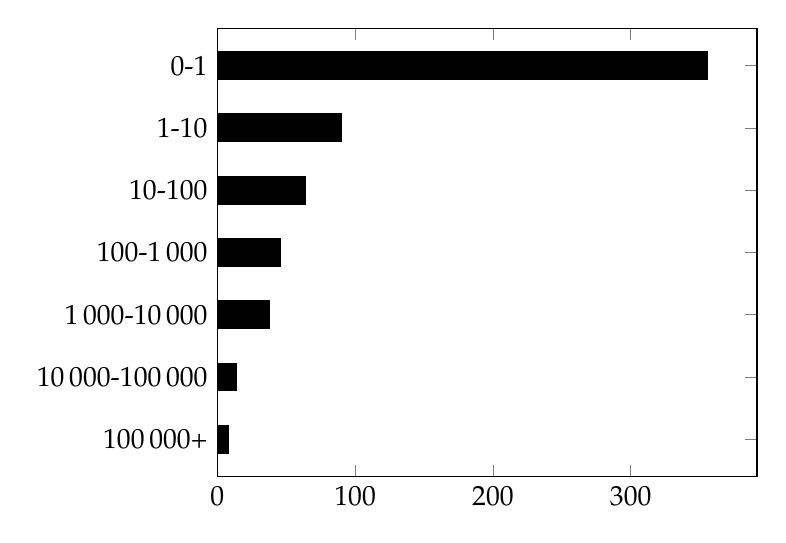
\begin{tikzpicture}
	\pgfplotstableread{
		Balance   			Contracts
		100\,000+			8
		10\,000-100\,000    14
		1\,000-10\,000      38
		100-1\,000      	46
		10-100     			64
		1-10				90
		0-1					356
		%0					3984
	}\datatable
	
	\begin{axis}[
	xbar stacked,   % Stacked horizontal bars
	xmin=0,         % Start x-axis at 0
	ytick=data,     % Use as many tick labels as y coordinates
	yticklabels from table={\datatable}{Balance}
	]
	\addplot [fill=black] table [x=Contracts, y expr=\coordindex] {\datatable};
	\end{axis}
	\end{tikzpicture}
	\label{BalancesFigure}
\end{figure}

The contract balances differ significantly (see Figure~\ref{BalancesFigure}).
The vast majority ($3\,984$,~or $86.6\%$)~of contracts have a zero balance.
One contract holds over one~million ether ($1\,500\,000$, or \$$440$~million at the time of testing), which accounts for~$38.4\%$~of the total balance of all contracts.
Contracts have from $1$~to $2\,525$~lines of code, with an average of $334$~lines and a median of $221$~lines.

\let\letcs\texapiletcs
\begin{figure}
	\caption{Findings on the big dataset \\ (excluding {\usevalue SolidityVisibility:name })}
	\centering
	\resizebox{0.8\textwidth}{!}{
	\begin{tikzpicture}[x={(.001,0)}, font=\large]
	\definecolor{darkgray}{RGB}{128,128,128}
	\definecolor{lightgray}{RGB}{232,232,232}
	\foreach  \l/\x/\c[count=\y] in {
		{\usevalue SolidityBytesByte:name }					/{\usevalue SolidityBytesByte:occur }				/lightgray,
		{\usevalue SolidityRedundantFallbackReject:name }	/{\usevalue SolidityRedundantFallbackReject:occur }	/lightgray, 
		{\usevalue SolidityLockedMoney:name }				/{\usevalue SolidityLockedMoney:occur }				/lightgray, 
		{\usevalue SolidityMaliciousLibraries:name }		/{\usevalue SolidityMaliciousLibraries:occur }		/lightgray, 
		{\usevalue SolidityErc20ApiViolation:name }			/{\usevalue SolidityErc20ApiViolation:occur }		/lightgray, 
		{\usevalue SolidityPrivateModifier:name }			/{\usevalue SolidityPrivateModifier:occur }			/lightgray, 
		{\usevalue SolidityStyleGuideViolation:name }		/{\usevalue SolidityStyleGuideViolation:occur }		/lightgray, 
		{\usevalue SolidityIntegerDivision:name }			/{\usevalue SolidityIntegerDivision:occur }			/lightgray, 
		{\usevalue SolidityPragmasVersion:name }			/{\usevalue SolidityPragmasVersion:occur }			/lightgray, 
		%{\usevalue SolidityUncheckedMath:name }			/{\usevalue SolidityUncheckedMath:occur }			/lightgray,
		%{\usevalue SolidityVisibility:name }				/{\usevalue SolidityVisibility:occur }				/lightgray, 
		{\usevalue SolidityBalanceEquality:name }			/{\usevalue SolidityBalanceEquality:occur }		/darkgray,
		{\usevalue SolidityTxOrigin:name }					/{\usevalue SolidityTxOrigin:occur }			/darkgray, 
		{\usevalue SolidityVar:name }						/{\usevalue SolidityVar:occur }					/darkgray,
		{\usevalue SolidityGasLimitAndLoops:name }			/{\usevalue SolidityGasLimitAndLoops:occur }	/darkgray, 
		{\usevalue SoliditySend:name }						/{\usevalue SoliditySend:occur }				/darkgray, 
		{\usevalue SolidityTimestampDependence:name }		/{\usevalue SolidityTimestampDependence:occur }	/darkgray, 
		{\usevalue SolidityDosWithThrow:name }				/{\usevalue SolidityDosWithThrow:occur }		/darkgray,
		{\usevalue SolidityCallValue:name }					/{\usevalue SolidityCallValue:occur }				/black,
		{\usevalue SolidityUncheckedCall:name }				/{\usevalue SolidityUncheckedCall:occur }			/black, 
		{\usevalue SolidityReentrancyExternalCall:name }	/{\usevalue SolidityReentrancyExternalCall:occur }	/black}
	{\node[left] at (0,\y) {\l};
		\fill[\c] (0,\y-.4) rectangle (\x,\y+.4);
		\node[right] at (\x, \y) {\x};}
	\draw (0,0) -- (8000,0);
	\foreach \x in {2000, 4000, ..., 8000}
	{\draw (\x,.3) -- (\x,0) node[below] {\x};}
	\draw (0,0) -- (0,19.4);
	\end{tikzpicture}}	
	\label{MassiveTestingFigure}
\end{figure}
\let\letcs\etoolboxletcs

SmartCheck analyzed the dataset in $7\,644$~seconds (approximately $2$~hours and $7$~minutes, or $437$~lines per second\footnote{Intel~Core~i5-4210M @ 2.60~GHz, 12~GB RAM, Windows~8.1 64~bit}).
As per SmartCheck, $99.9\%$~of contracts have issues, $63.2\%$~of contracts have critical vulnerabilities\footnote{The issues found by SmartCheck in the big dataset were not manually verified.}.
The findings are presented in Table~\ref{MassiveTestingTable} and Figure~\ref{MassiveTestingFigure} (colors denote severity levels: black -- high, dark gray -- medium, light gray -- low).
The most prevalent issue, \textbf{\let\letcs\texapiletcs \usevalue SolidityVisibility:name \let\letcs\etoolboxletcs} (detected~{\let\letcs\texapiletcs \usevalue SolidityVisibility:occur \let\letcs\etoolboxletcs} times, which accounts for $67.30\%$~of all findings), is excluded from the figure for clarity.

\let\letcs\texapiletcs
\begin{table}[t]
	\centering
	\caption{Code issues detected on a big dataset}
	\begin{tabular}{|c|l|r|r|}
		\hline
		\textbf{Severity} & \textbf{Pattern} & \textbf{Findings} & \textbf{\% of all} \\
		\hline
		\multirow{3}{*}{high} & {\usevalue SolidityReentrancyExternalCall:name } & {\usevalue SolidityReentrancyExternalCall:occur } & $3.329$ \\
		 & {\usevalue SolidityUncheckedCall:name } & {\usevalue SolidityUncheckedCall:occur } & $0.818$ \\
		 & {\usevalue SolidityCallValue:name } & {\usevalue SolidityCallValue:occur } & $0.228$ \\
		\hline
		\multirow{8}{*}{medium} & {\usevalue SolidityDosWithThrow:name } & {\usevalue SolidityDosWithThrow:occur } & $6.521$ \\
		& {\usevalue SolidityTimestampDependence:name } & {\usevalue SolidityTimestampDependence:occur } & $6.378$ \\
		& {\usevalue SoliditySend:name } & {\usevalue SoliditySend:occur } & $2.794$ \\
		& {\usevalue SolidityGasLimitAndLoops:name } & {\usevalue SolidityGasLimitAndLoops:occur } & $2.164$ \\
		& {\usevalue SolidityVar:name } & {\usevalue SolidityVar:occur } & $0.529$ \\
		& {\usevalue SolidityTxOrigin:name } & {\usevalue SolidityTxOrigin:occur } & $0.163$ \\
		& {\usevalue SolidityBalanceEquality:name } & {\usevalue SolidityBalanceEquality:occur } & $0.094$ \\
		\hline
		\multirow{10}{*}{low} & {\usevalue SolidityVisibility:name } & {\usevalue SolidityVisibility:occur } & $67.296$ \\& {\usevalue SolidityPragmasVersion:name } & {\usevalue SolidityPragmasVersion:occur } & $3.067$ \\
		& {\usevalue SolidityIntegerDivision:name } & {\usevalue SolidityIntegerDivision:occur } & $1.432$ \\
		& {\usevalue SolidityStyleGuideViolation:name } & {\usevalue SolidityStyleGuideViolation:occur } & $1.348$ \\
		& {\usevalue SolidityPrivateModifier:name } & {\usevalue SolidityPrivateModifier:occur } & $1.014$ \\
		& {\usevalue SolidityErc20ApiViolation:name } & {\usevalue SolidityErc20ApiViolation:occur } & $1.169$ \\
		& {\usevalue SolidityMaliciousLibraries:name } & {\usevalue SolidityMaliciousLibraries:occur } & $1.157$ \\
		& {\usevalue SolidityLockedMoney:name } & {\usevalue SolidityLockedMoney:occur } & $0.439$ \\
		& {\usevalue SolidityRedundantFallbackReject:name } & {\usevalue SolidityRedundantFallbackReject:occur } & $0.053$ \\
		& {\usevalue SolidityBytesByte:name } & {\usevalue SolidityBytesByte:occur } & $0.006$ \\
		\hline
	\end{tabular}
	\label{MassiveTestingTable}
\end{table}
\let\letcs\etoolboxletcs


%%%% SECTION 5: RELATED WORK %%%%
\section{Related work} \label{RelatedWork}

Multiple tools aim at improving the security and correctness of Ethereum smart contracts.
Static checks are built into the online Solidity compiler Remix~\cite{BrowserSolidity}.
Oyente~\cite{Luu2016} is a symbolic execution tool vulnerability detection in EVM bytecode.
Securify~\cite{Tsankov2018} analyzes Solidity source code as well as EVM bytecode. % not really sure what Securify does under the hood
\cite{Bhargavan2016} and \cite{Pettersson2016} propose writing Ethereum contracts in safer languages (F* and Idris respectively).
\cite{Hirai2017} describes existing attempts to formal verification of EVM bytecode as well as the EVM itself.
%\cite{DrYAnalyzer} and \cite{Luu16} use symbolic execution to analyze EVM bytecode.
\cite{Hildenbrandt2018} formally describes the full semantics of the EVM, providing the foundation for formal verification tools for EVM bytecode .


%%%% SECTION 6: CONCLUSION %%%%
\section{Conclusion and future work}
	
We provided a comprehensive overview and classification of code issues in Solidity -- the major high-level language for Ethereum smart contracts.
We implemented SmartCheck -- an efficient static analysis tool for Solidity, which offers significant improvements over existing alternatives.
We tested our tool on a massive set of real-world contracts and detected code issues in the vast majority of them.
The tool can be improved in multiple directions: improving the grammar\footnote{The currently used grammar failed to parse $0.16\%$~of lines in our dataset.}, making patterns more precise (e.g.,~the temporarily muted {\usevalue SolidityUncheckedMath:name }), adding new patterns, implementing more sophisticated static analysis methods, adding support for other languages.

Security is still an issue in blockchain development.
We hope that SmartCheck will help solve this major challenge by providing smart contract developers with fast and relevant feedback on potentially problematic source code patterns.

\chapter{Privacy-preserving KYC on Ethereum}

\label{Chapter12KYC}

In this Chapter, we describe the current approach to identity management and propose KYCE -- a privacy-preserving KYC scheme for token whitelisting on Ethereum.\footnote{This Chapter is based on~\cite{Biryukov2018}, which, in turn, described a hackathon project. The team consisting of Daniel Feher, Dmitry Khovratovich, Sergei Tikhomirov, Aleksei Udovenko, and Maciej \.{Z}urad implemented a proof-of-concept implementation in May~2017 during the Luxblock hackathon in Luxembourg and won a joint first prize. Contributions of the author of this thesis include: implementing parts of the hackathon project and writing the paper (except for Section~\ref{sec:PrivacyPreservingKYC}).}


\section{Identity}

Digital identity is the information used by a computer system to represent a user.
Access to services is controlled in two steps:

\begin{itemize}
	\item authentication: a user proves that they are who they claim to be;
	\item authorization: the system ensures that the user has the right to perform the requested action.
\end{itemize}

To comply with regulations, financial institutions verify the identities of their customers.
Modern finance depends on government-issued identities.
Regulations in most jurisdictions demand that banks obtain proof of identity from customers before doing business with them -- a procedure known as "know your customer," or KYC.
"Anti money laundering" (AML) and "counter terrorist financing" (CTF) are related regulations that require banks to stop and report suspicious transactions.

Modern KYC practices weaken users' control over their personal information and threaten their privacy.
Financial institutions store sensitive information in private databases, which become a target for corrupt employees or external hackers.
Independent KYC/AML implementations lead to high compliance cost and multiply the risk of identity theft.

Open blockchains like Ethereum take a more decentralized approach to identity management.
Users join these networks without any identification.
Financial service providers establish consortia to apply blockchain technologies in their services~\cite{EEA2017, Hyperledger, R3}.
To comply with regulation, they have to handle government-issued identities in a blockchain setting.
This non-trivial task becomes more challenging, considering users' demands for stronger privacy protection.
The European privacy regulation (GDPR~\cite{GDPR16}) that came into force in May~2018 poses more challenges for organizations that handle personal data.

In this work, we first explore the centralized and decentralized approaches to identity.
We then propose KYCE -- a privacy-preserving Ethereum-based KYC implementation.
KYCE allows banks to implement KYC checks using an external smart contract -- a KYC provider.
Our scheme uses zero-knowledge proofs to check users' eligibility without disclosing their private information to anyone except the KYC provider.
A smart contract stores the KYC whitelist in the form of a cryptographic accumulator.
This construction allows users to be efficiently added to, removed from, and checked against the list without storing any plaintext data on the blockchain.
We then discuss possible use cases and implementation challenges.

\subsection{Centralized identity}

In terms of asymmetric cryptography, identity~$I$ of user~$U$ is a public-private key pair~$(pub_U, priv_U)$.
The public key~$pub_U$ authenticates the user (or, equivalently, links their current action to some past actions).
Public identifiers like username or address are derived from~$pub_U$.
The private key~$priv_U$ allows $U$ to sign messages on behalf of~$I$.
For the system, $U$ is whoever possesses $priv_U$.

In the centralized identity model, prevalent on the Internet today, users delegate managing their private keys to a trusted party and use a password to access them when necessary.
This approach is sub-optimal in many regards.
First, users do not control their identities.
The trusted party always has the technical ability to sign messages without the user's consent or to prevent the user from signing the message they want.
Moreover, users' data is stored by a centralized entity, providing incentives for an attack.
Finally, users have to create a new identity for each website they wish to register with.
As a result, they adhere to a risky practice of reusing passwords.
Third-party login protocols such as OAuth and OpenID~\cite{Dodanduwa2018} partially address this issue ("login with").
In this scheme, a website queries the service that holds the user's existing identity (e.g.,~Google) and asks for permission to access a subset of the user's data (e.g.,~name and email).
This approach alleviates the password management problem but increases the impact of potential identity theft.

Though users can revoke access at any time, the "login with" scheme is still privacy-violating.
Imagine a user who reveals their birth date to prove to a website that they are 18 years of age or older.
If they later revoke the access, their date of birth will never change.
Thus, they grant the third-party website effectively unlimited access to a piece of private information.

Maintaining correspondence between "real world" identities and public keys has long been a challenge.
Widely deployed centralized solutions like PKI suffer from risks associated with centralization: a fraudulent authority can issue rogue certificates~\cite{Amann2017}.


\subsection{Decentralized identity and open blockchains}

The PGP "web of trust" is a noteworthy attempt at creating a decentralized identity system~\cite{Feisthammel2017}.
It has not gained significant traction due in part to usability challenges~\cite{Ruoti2015} and concerns about the security of the long-term key model~\cite{Valsorda2016}.

Bitcoin~\cite{Nakamoto2008} eliminates the problem of connecting public keys to identities in a radical manner: a user may generate many public keys that \textit{are} identities.
Alternative blockchains such as Ethereum~\cite{Buterin2014, Wood2014} take a similar approach.
The way open blockchains handle identity may come at odds with financial regulation.
We propose a design that will simultaneously leverage the power of blockchain-based smart contracts, enable banks to implement KYC to comply with the law, and preserve users' privacy.


\subsection{Financial and privacy regulation in the EU} \label{sec:Ch12KYCEU}

The current EU legislation "on information accompanying transfers of funds" came into effect in 2015~\cite{EU847}.
In the wake of the rapid growth of cryptocurrencies, the EU is tightening its anti-money laundering regulations, stating that "virtual currency exchange platforms and custodian wallet providers will have to apply customer due diligence controls, ending the anonymity associated with such exchanges"~\cite{EU16}.
See~\cite{Vandezande2017} for the analysis of virtual currencies under the EU AML law.

In 2018, two pieces of legislation came into force in the EU\@.

\begin{itemize}
	\item The \textbf{Revised Payment Service Directive} (PSD2) obligates banks to provide access to their customers' accounts through open APIs~\cite{Hellstroem2017}.
	This measure is meant to foster competition and give rise to third-party financial service providers.
	For instance, a unified banking API would simplify connecting banking infrastructure to open blockchains~\cite{Elison2016}.
	\item The \textbf{General Data Protection Regulation} (GDPR) harmonizes data privacy laws across the EU~\cite{GDPR16} and introduces stricter rules for handling data of EU residents even for companies from outside the EU\@. We refer the reader to~\cite{Berberich2016} describes possible implications of blockchain adoption from the viewpoint of the EU data protection regulation.
\end{itemize}


\section{KYCE: a decentralized KYC-compliant exchange}

KYC requirements differ depending on jurisdiction~\cite{PWC2015}.
A typical KYC procedure links users' real-world identities to their accounts and checks users against a whitelist or a blacklist.
The details of the KYC procedure do not affect our design.

\subsection{Definitions and security properties}

\begin{definition}
	A \textbf{KYC procedure} is a process that determines if a given user is eligible for a given transaction.
\end{definition}

\begin{definition}
	A \textbf{KYC provider} is an entity that performs a KYC procedure.
\end{definition}

\begin{definition}
	A \textbf{financial service} is an information system that allows users to exchange units of value.
\end{definition}

\begin{definition}
	A financial service is \textbf{KYC-compliant} w.r.t.~the KYC procedure if and only if all users are eligible for all transactions they perform.
\end{definition}

\begin{definition}
	A KYC-compliant financial service is \textbf{privacy-preserving} if and only if only the KYC provider has access to the users' private data.
\end{definition}


\subsection{Tokens and exchanges}

Our KYC solution can be applied for any service.
For concreteness, consider a token exchange as an example.

\begin{definition}
	A \textbf{token} is a transferable fungible unit of value maintained by a smart contract.
\end{definition}

ERC20~\cite{Victor2019} is the de-facto standard API for implementing token contracts in Ethereum.
A token contract keeps track of users' token balances and allows them to transfer tokens using the following functions:

\begin{itemize}
	\item \texttt{transfer} sends a given amount of tokens to a given address;
	\item \texttt{approve} allows a given user to withdraw up to a given amount of tokens from the account of the user calling the function;
	\item \texttt{transferFrom} sends a given amount of tokens from one given address to another (the amount has to be \texttt{approve}d beforehand).
\end{itemize}

\begin{definition}
	An \textbf{exchange} is a service that allows users to exchange tokens.
\end{definition}

Centralized exchanges, implemented as regular web services, are the most prevalent.
We are mostly interested in decentralized, or on-chain exchanges, implemented as smart contracts.

An exchange without KYC support may be used as follows.
\begin{enumerate}
	\item Alice creates an order to sell $X$~A-tokens for $Y$~B-tokens;
	\item Bob creates an order to sell $Y$~B-tokens for $X$~A-tokens;
	\item The exchange matches the two orders and transfers (by calling \texttt{transferFrom}) $X$~A-tokens from Alice to Bob and~$Y$~B-tokens from Bob to Alice.
\end{enumerate}

The transaction succeeds if Alice and Bob have \texttt{approve}d the exchange with a sufficient amount of A- and B-tokens, respectively, before \texttt{transferFrom} is called.
Users withdraw tokens from the exchange by calling \texttt{approve(exchangeAddress,0)}.



\subsection{Privacy-preserving KYC}
\label{sec:PrivacyPreservingKYC}

We propose KYCE -- a privacy-preserving KYC design for Ethereum-based financial service providers.
A KYC contract provides an API to other contracts so that external services can determine if a given user is KYC-approved for using a given token.
A KYC provider (a governmental entity or company in charge of customer onboarding) performs the necessary checks for a new customer and adds their address to the whitelist.

A simple approach to implementing a KYC check with a separate contract would be the following.
The KYC contract stores the whitelist of approved addresses.
On every \texttt{transfer}, the token contract checks if the address belongs to the whitelist.
This design has a fundamental privacy flaw: the contract stores all whitelisted addresses on-chain in plaintext.
Moreover, users must use the same addresses they have registered with the KYC provider.
Address reuse threatens privacy: an adversary can link the user's transactions using public blockchain data.

\paragraph{Our approach}
We use cryptographic techniques to design a privacy-preserving KYC solution.
In KYCE, the KYC contract stores a \textbf{cryptographic accumulator} of the whitelisted addresses.

A cryptographic accumulator~$A$ absorbs certain algebraic objects and provides an interface to generate and verify zero-knowledge proofs that a given value has been accumulated.
In our construction, to generate a proof for value~$x\in A$, one needs a \textit{witness} that depends on~$A$ and~$x$.
The accumulator owner provides the witness to the user who submitted $x$.
We suggest an accumulator based on bilinear maps~\cite{Camenisch2009}.

The KYC workflow is as follows.
The KYC provider publishes a smart contract and initializes it with an empty accumulator.
The User interacts with the KYC provider physically or online and provides the credentials needed to pass the verification.
The User also generates their own master secret~$m$ and during the authenticated session, gives the provider a Pedersen commitment~$g_1^m\cdot g_2^r$ to it.
$g_1$ and~$g_2$ are certain group generators,\footnote{Here and in the further text all multiplications take place in the pre-selected group of prime order~$q$, typically an elliptic-curve group.} and~$r$ is random.
If the User passes the procedure, the provider updates the accumulator with user-dependent data and gives the User a witness.
In every subsequent Ethereum transaction to KYCE, the User provides a proof that they have been registered in the accumulator, that this right has not been revoked, and that the proof owner and the transaction sender are one person.
KYCE verifies the last statement.
The KYC contract verifies the rest against the current accumulator value.
If the checks pass, KYCE executes the requested action.

\paragraph{Details on the accumulator construction}
We construct an accumulator based on a pairing function~$e(\cdot,\cdot)$ in some pairing setting.\footnote{The original paper~\cite{Camenisch2009} uses type-1 pairings, but type-3 pairings can be adopted as well.}
The accumulator contains the serial numbers, possibly consecutive integers.\footnote{It is possible to store public keys, but it would be less efficient.}

The accumulator is constructed as follows.
We assume a bilinear pairing~$e:\,G\times G\rightarrow G_T$, where $G,G_T$ are groups of order~$q$.
The KYC provider selects a generator~$g$ and a secret value $\gamma\overset{\$}{\leftarrow} \mathbb{Z}_q$.
It also selects $L$ as an upper bound of users enabled for KYC and computes $z = e(g,g)^{\gamma^{L+1}}$.
It initialized the accumulator value~$\mathrm{A}$ by $1$.

Let us denote $g_i = g^{\gamma^i}$.
The provider publishes $\mathrm{A},\{g_i\}_{1\leq i\leq L, \,L+2\leq i \leq 2L}$, the set of registered KYC indices $V=\emptyset$, and the parameters $g,z$ needed for verification.

Every User who passes the KYC check is issued a new serial number~$i$, the witness~$w_i = \prod_{j\in V,j\neq i} g_{L+1-j+i}$, where $V$ is the set of all issued serial numbers, and a signature~$\sigma_i$ of~$g_i||i$ on the provider's private signature key.
The witness is used to generate a proof of accumulating.\footnote{We refer an interested reader to~\cite{Camenisch2009} for the details.}
The KYC provider updates the accumulator with~$i$ by
$$
\mathrm{A_{V\cup\{i\}}} \leftarrow \mathrm{A_V} \cdot g_{L+1-i}
$$
multiplying it by $g_{L+1-i} = g^{\gamma^{L+1-i}}$, and~$i$ is published as a new valid serial number.
To prove that $i$ has been committed to $A$ and has not been revoked without disclosing it, the holder of~$w_i$ updates it\footnote{We omit the details, but the update can be performed just before the presentation, not necessarily after every accumulator update.} so that the following equation holds:
$$
\frac{e(g_i, A)}{e(g,w_i)} = z.
$$

Note that revocation is also efficient.
The KYC contract owner simply multiplies the accumulator value by the inverse of~$g_{L+1-i}$.
The witness value cannot be updated anymore.

\paragraph{Presentation} 
When issuing a transaction to use the exchange (e.g.,~create an order), the user submits a \textbf{zero-knowledge proof} of the following statement:
\begin{itemize}
	\item I know the private key of the current user address (\texttt{msg.sender}), and
	\item I know a signature~$\sigma_i$ and a witness~$w_i$ for some number~$i$ that has been accumulated in the
	accumulator~$A$ in the KYC contract.
\end{itemize}
This compound statement must be \textit{atomic}, i.e.,~the sub-statements cannot be extracted as separate valid proofs, as this would make the transaction malleable.

The atomicity (and non-malleability) are ensured as follows.
Let us denote the proof of knowledge for the witness and signature by~$PK_w$.
Then the Prover submits 
$$
P = \{PK_w \wedge PK_s\},
$$
where $PK_s$ is the proof of knowledge of the private key of the \texttt{msg.sender}'s ECDSA public key, which can be taken from~\cite{Chase2016}.
The technique to make a composite proof of knowledge (PoK) is straightforward, as both PoKs are non-interactive, and is standard in complex PoK protocols:
\begin{enumerate}
	\item The Prover collects a set $\mathcal{C}$ of commitments asserted in sub-proofs $PK_w$ and~$PK_s$.
	\item The Prover makes necessary randomization of~$\mathcal{C}$ to create $t$-values $\mathcal{T}$.
	\item The Prover computes $c \leftarrow H(\mathcal{C},\mathcal{T})$.
	\item The Prover computes $s$-values $\mathcal{S}$ using
	$\mathcal{C}$, $\mathcal{T}$, and~$c$.
	\item The proof~$P$ is $(\mathcal{C}, \mathcal{S},c)$.
	To verify it one computes asserted $t$-values $\widehat{\mathcal{T}}$ and verifies
	$$
	c\overset{?}{=}H(\mathcal{C},\widehat{\mathcal{T}}).
	$$
\end{enumerate}

The resulting proof~$P$ is submitted as an Ethereum transaction argument.
KYCE retrieves the current accumulator value and verifies $P$ against it and the message sender's public key, available in the transaction metadata.
If the proof is correct, the order is executed.


\subsection{Use cases}

Either the exchange contract or the token contract must be KYC-compliant -- i.e.,~check the eligibility of transacting parties using the introduced cryptographic scheme using the KYC contract.

\paragraph{KYC-compliant exchange}

If the exchange is KYC-compliant, the tokens do not need to be aware of the KYC (Figure~\ref{fig:KYCCompliantExchange}).

\begin{figure}[h]
	\centering
	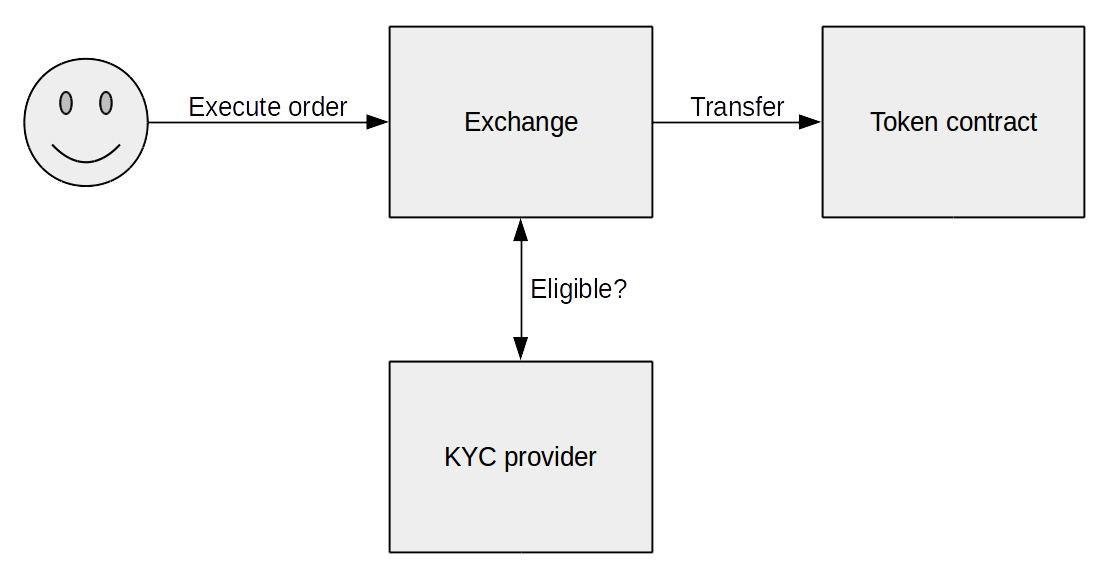
\includegraphics[width=0.8\textwidth]{figure-kyc-exchange}
	\caption{KYC-compliant exchange.}
	\label{fig:KYCCompliantExchange}
\end{figure}

Consider an established exchange that trades dozens of tokens.
It applies for official approval in a jurisdiction that requires all customers to pass the KYC procedure.
The governmental body acts as a KYC provider, deploys a KYC contract, and publishes its address.
The exchange adds KYC checks to its codebase and continues operation.
Users who do not want to apply for KYC can withdraw their tokens from the exchange.


\paragraph{KYC-compliant token}

If the token is KYC-compliant, the exchange does not need to be aware of the KYC (Figure~\ref{fig:KYCCompliantToken}).

\begin{figure}[h]
	\centering
	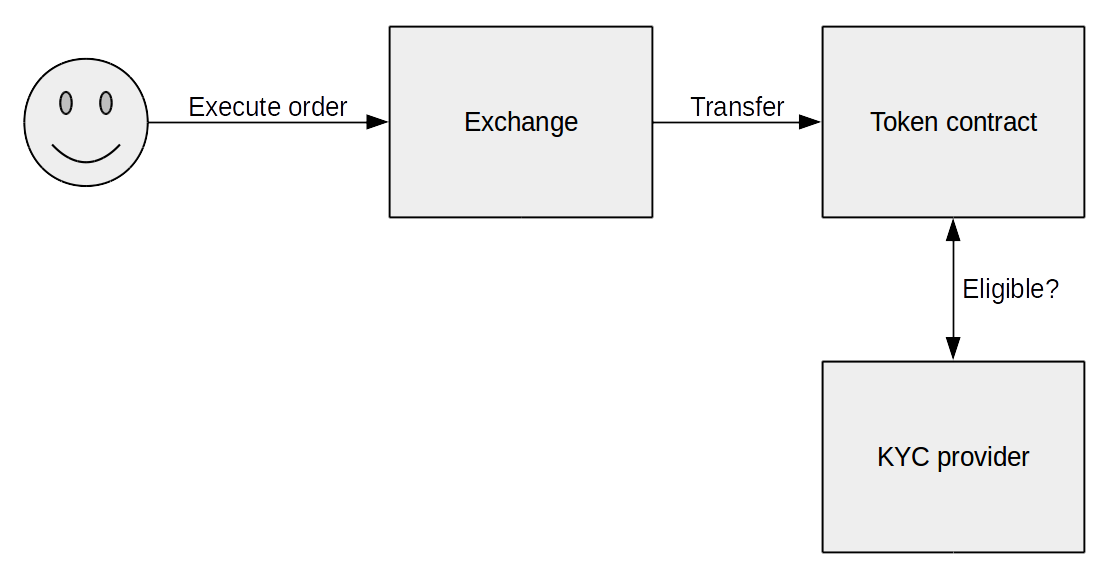
\includegraphics[width=0.8\textwidth]{figure-kyc-token}
	\caption{KYC-compliant token.}
	\label{fig:KYCCompliantToken}
\end{figure}

Consider a government that issues its own tokens.\footnote{Bank of England~\cite{Danezis2016} and the Monetary Authority of Singapore~\cite{Singapore17} have already researched this direction.}
KYC-approved users could use government tokens for tax payments, fees, and fines.
Such a solution leverages smart contracts' flexibility and auditability while only allowing approved entities to use the token.
The KYC-enabled government token can also be traded on exchanges, which would allow citizens to hold currency portfolios of their choice and only purchase government tokens to transact with the state.

\paragraph{Transaction-dependent checks}

Many jurisdictions impose restrictions that depend on the value of the transaction.
E.g.,~the EU regulation~\cite{EU847} states that "the obligation to check whether information on the payer or the payee is accurate should \textelp{} be imposed only in respect of individual transfers of funds that exceed \EUR{1\,000}".
EU member states impose further restrictions for large transactions, e.g.,~exceeding \EUR{10\,000} in Belgium, \EUR{15\,000} in Germany and in the Netherlands~\cite{PWC2015}.
Either the exchange contract or the token contract can perform such checks by storing the following mappings:
\begin{itemize}
	\item address $=>$ accumulated transaction volume in the current period (day, month, year);
	\item address $=>$ timestamp of the latest transaction.
\end{itemize}


\section{Implementation details}

We have created an initial (not privacy-preserving) implementation of the proposed design.
Our project consists of two smart contracts written in Solidity: KycProvider and KyceToken.
KycProvider maintains a 2-dimensional boolean array that stores the eligibility status across users and tokens.
On initialization, the address that deploys the contract is appointed as the \textit{owner}, allowing it to add and remove users from the whitelist.
The ownership may be transferred (using the functionality inherited from the standard \texttt{Ownable} contract).

The KycProvider exposes the following API:

\begin{itemize}
	\item \texttt{add(address \_user, address \_token)} makes the user eligible for using the token (callable only by the owner);
	\item \texttt{remove(address \_user, address \_token)} makes the user not eligible for using the token (callable only by the owner);
	\item \texttt{isEligible(address \_user, address \_token)} checks if the user is eligible for using the token.
\end{itemize}

KyceToken adheres to the de-facto standard token API in Ethereum -- ERC20.
To minimize the risk of security issues due to implementation subtleties, we inherit a widely used and tested ERC20 implementation by OpenZeppelin.
We override the functions \texttt{approve}, \texttt{transfer}, and \texttt{transferFrom} to check if the given user (\texttt{msg.sender}) is eligible for using this token.
If \texttt{isEligible} returns \texttt{false}, the execution stops.
If it returns \texttt{true}, the corresponding function of the superclass is invoked.

The implementation of the proposed scheme requires certain cryptographic primitives.
Some of them are partially available in Ethereum as pre-compiled contracts (elliptic curve addition, scalar multiplication, and pairing checks).
For the proposed scheme to be fully implemented, pairing evaluation is also required.\footnote{As of 2020, Ethereum does not support pairing evaluation.}


\section{Related work}

Jos{\'{e}} Parra Moyano and Omri Ross use distributed ledgers to improve the KYC process~\cite{Moyano2017}.
Their proposal can be summarized as follows:
\begin{itemize}
	\item the regulator maintains a database with all users' private data;
	\item the user signs a contract with their first bank (the \textit{home bank});
	\item the home bank stores hashes of the user's documents in a smart contract in a permissioned blockchain;
	\item when the user signs a contract with another bank it obtains the user's documents from the database and looks up the hash to ensure that the user has been KYC-approved;
	\item the identity of the home bank is not revealed;
	\item a cost-sharing mechanism for banks allows them to proportionally share the cost of the initial KYC approval.
\end{itemize}
In this design, all banks store users' private data -- contrary to our solution, where it is stored only with the KYC provider.
The authors also propose a more decentralized design but claim it to be of lesser practical relevance.

Clare Sullivan and Eric Burger investigate possible implications of further development of the Estonian e-residency program using blockchain technology~\cite{Sullivan2017}.
E-residency of Estonia is a governmental program that provides applicants with a digital identity that can be used, e.g.,~to register a company and open a bank account.
Estonian e-residency disconnects a digital identity from citizenship or physical residence.
Within the e-residency program, Estonia collaborates with a blockchain project Bitnation~\cite{Bitnation15, Estonia15}.
Provable (previously known as Oraclize) offers a connector that lets Ethereum contracts handle e-residency identities~\cite{Provable}.

A project~\cite{Ohtamaa2016} similar to ours implements a KYC scheme using Ethereum, but stores the KYC status on-chain in plaintext.
Multiple projects aim at easing customer onboarding for banks~\cite{CambridgeBlockchain, KycChain, SnapSwap, Tradle}.
Blockchain consortium R3 has developed a proof-of-concept implementation of a shared KYC between ten banks based on its blockchain platform Corda~\cite{Allison2016}.
Multiple Ethereum-based identity projects have been proposed~\cite{Mesropyan2017, Sovrin, Uport}.


\section{Conclusion}

We have proposed a modular design of an Ethereum-based financial service with an external KYC check, which benefits all participants.

\begin{itemize}
	\item \textbf{Users} obtain a unified identity that they can use with multiple financial services.
	Users' data is stored only with the KYC provider and can be easily updated.
	Personal data is neither stored on the blockchain nor transmitted to third parties.
	\item \textbf{Financial services} greatly simplify the KYC process: it boils down to a single API call.
	Our design lets them cut KYC costs while at the same time diminishing risks of handling sensitive data.
	\item \textbf{Governments} get an opportunity to stimulate innovation in the financial sector by providing a unified and simple KYC API, which is especially relevant in rapidly growing fintech and blockchain industries.
\end{itemize}

Our design is agnostic to the nature of the entity behind the KYC contract.
It does not have to be a government body.
The proposed solution can be used in any setting where a smart contract based service wants to limit the set of its users.
For instance, many jurisdictions (e.g.,~the~US~\cite{SEC}) only allow certain investments to be offered to "accredited investors."
These are typically high-net-worth individuals and financial institutions.
This logic can be replicated in a blockchain setting.
Consider a blockchain-based financial service that only accepts cryptocurrency users who possess more than $10\,000$~USD and have done their first transaction before~2017.
The "accrediting" functionality is delegated to a third party KYC provider.
Proving net worth and previous activity on the blockchain is straightforward.
More checks can be added.
Once accredited, an investor can use multiple "restricted" services without revealing any personal details to their developers.


\bookmarksetupnext{level=chapter}
\chapter{Conclusion}

\label{Chapter13Conclusion}

We have studies various aspects of security and privacy of various blockchain protocols and applications, in particular Bitcoin, Ethereum, and the Lightning Network.

\todo[inline]{Outline future directions and open questions}
%\fi
%----------------------------------------------------------------------------------------
%	THESIS CONTENT - APPENDICES
%----------------------------------------------------------------------------------------

\appendix % Cue to tell LaTeX that the following "chapters" are Appendices

% Include the appendices of the thesis as separate files from the Appendices folder
% Uncomment the lines as you write the Appendices

%\include{Appendices/AppendixA}
%\include{Appendices/AppendixB}
%\include{Appendices/AppendixC}

%----------------------------------------------------------------------------------------
%	BIBLIOGRAPHY
%----------------------------------------------------------------------------------------

\printbibliography[heading=bibintoc]

%----------------------------------------------------------------------------------------

\end{document}  
